% Tell RStudio that weaving is to be done with the knitr package
% !Rnw weave = knitr


%\listfiles                   %% Show all files used in the book
\documentclass[11pt]{book}\usepackage[]{graphicx}\usepackage[]{color}
%% maxwidth is the original width if it is less than linewidth
%% otherwise use linewidth (to make sure the graphics do not exceed the margin)
\makeatletter
\def\maxwidth{ %
  \ifdim\Gin@nat@width>\linewidth
    \linewidth
  \else
    \Gin@nat@width
  \fi
}
\makeatother

\definecolor{fgcolor}{rgb}{0.345, 0.345, 0.345}
\newcommand{\hlnum}[1]{\textcolor[rgb]{0.686,0.059,0.569}{#1}}%
\newcommand{\hlstr}[1]{\textcolor[rgb]{0.192,0.494,0.8}{#1}}%
\newcommand{\hlcom}[1]{\textcolor[rgb]{0.678,0.584,0.686}{\textit{#1}}}%
\newcommand{\hlopt}[1]{\textcolor[rgb]{0,0,0}{#1}}%
\newcommand{\hlstd}[1]{\textcolor[rgb]{0.345,0.345,0.345}{#1}}%
\newcommand{\hlkwa}[1]{\textcolor[rgb]{0.161,0.373,0.58}{\textbf{#1}}}%
\newcommand{\hlkwb}[1]{\textcolor[rgb]{0.69,0.353,0.396}{#1}}%
\newcommand{\hlkwc}[1]{\textcolor[rgb]{0.333,0.667,0.333}{#1}}%
\newcommand{\hlkwd}[1]{\textcolor[rgb]{0.737,0.353,0.396}{\textbf{#1}}}%

\usepackage{framed}
\makeatletter
\newenvironment{kframe}{%
 \def\at@end@of@kframe{}%
 \ifinner\ifhmode%
  \def\at@end@of@kframe{\end{minipage}}%
  \begin{minipage}{\columnwidth}%
 \fi\fi%
 \def\FrameCommand##1{\hskip\@totalleftmargin \hskip-\fboxsep
 \colorbox{shadecolor}{##1}\hskip-\fboxsep
     % There is no \\@totalrightmargin, so:
     \hskip-\linewidth \hskip-\@totalleftmargin \hskip\columnwidth}%
 \MakeFramed {\advance\hsize-\width
   \@totalleftmargin\z@ \linewidth\hsize
   \@setminipage}}%
 {\par\unskip\endMakeFramed%
 \at@end@of@kframe}
\makeatother

\definecolor{shadecolor}{rgb}{.97, .97, .97}
\definecolor{messagecolor}{rgb}{0, 0, 0}
\definecolor{warningcolor}{rgb}{1, 0, 1}
\definecolor{errorcolor}{rgb}{1, 0, 0}
\newenvironment{knitrout}{}{} % an empty environment to be redefined in TeX

\usepackage{alltt}
%\usepackage{amsmath}
\usepackage{array}            %% nicer arrays and tables
\usepackage{times}            %% PS Times, rather than CM fonts
\usepackage[T1]{fontenc}      %% for non-alpha chars in \tt
\usepackage{sfheaders}        %% Chap/Sec headers in Helvetica
\usepackage{graphicx}         %% well, its about graphics
\usepackage{alltt}            %% for source listings
\usepackage{mdwlist}          %% Compressed list environments: itemize*, description*, etc.
\usepackage{comment}          %% Stuff commented out
\usepackage{xspace}           %% Smart spacing after tex macros
\usepackage[obeyspaces]{url}  %% URLs and pathnames
\usepackage{bm}               %% for bold math symbols (via \vec{}, \mat{})
\usepackage[tc]{titlepic}     %% Used for the cover illustration
\usepackage{showlabels}       %% Used for checking xrefs
\renewcommand{\showlabelfont}{\footnotesize\ttfamily}
\usepackage{tikz}             %% used for hyp3way.tex
% colored tables
\usepackage{xcolor,colortbl}  %% used ub Ch 01
\usepackage{multirow}
%\usepackage[traceon]{changebar}  %% When we need to show diffs
\usepackage{epigraph}         %% section quotations
\setlength{\epigraphwidth}{.8\textwidth}
%% indexing
\usepackage{index}          

\usepackage[comma]{natbib}
\renewcommand{\bibname}{References}
%\bibliographystyle{abbrvnat-apa}  % this includes URLs
\bibliographystyle{abbrvnat-apa-nourl}


%%%%%%%%%%%%%%%%%%%%%%%%%%%%%%%%%%%%%%%%%%%%%%%%
%% Indexing -- only main index for now
%%%%%%%%%%%%%%%%%%%%%%%%%%%%%%%%%%%%%%%%%%%%%%%%

%\makeglossary
\usepackage{index}
\makeindex
\newindex{xmp}{ide}{ine}{Example Index}

%% Page Headings
\makeatletter
\usepackage{fancyhdr}
\pagestyle{fancy}
\addtolength{\headwidth}{\marginparsep}
\addtolength{\headwidth}{\marginparwidth}
\addtolength{\headheight}{1.6pt}   %% suppress overfull \vbox chatter
%
%% The next two lines are only for draft printing
\def\infoleft{\quad [{\small\ttfamily\@filef@und}]}
\def\inforight{[\number\month-\number\day-\number\year]\quad}
%
\renewcommand{\chaptermark}[1]{%
 \markboth{\thechapter\ #1}{}}
\renewcommand{\sectionmark}[1]{%
 \markright{\thesection\ #1}}
\lhead[\fancyplain{}{\bfseries\sffamily\thepage}]%
      {\fancyplain{}{{\bfseries\sffamily\rightmark}\infoleft}}
\rhead[\fancyplain{}{\inforight{\bfseries\sffamily\leftmark}}]%
      {\fancyplain{}{\bfseries\sffamily\thepage}}
\cfoot{}
\makeatother

%%%%%%%%%%%%%%%%%%%%%%%%%%%%%%%%%%%%%%%%%%%%%%%%
% Only for chapter.Rnw
\usepackage{xr}
\externaldocument{book}
%%%%%%%%%%%%%%%%%%%%%%%%%%%%%%%%%%%%%%%%%%%%%%%%


%  Page dimensions
\addtolength{\hoffset}{-1.1cm}
\addtolength{\textwidth}{2.2cm}
\addtolength{\voffset}{-2cm}
\addtolength{\textheight}{4cm}
\setlength{\parskip}{3pt plus 1pt}
\addtolength\marginparwidth {-.5cm}

% Float parameters
\renewcommand\textfraction{.15}
\renewcommand\topfraction{.8}
% the rest are the defaults
\setcounter{topnumber}{2}
\setcounter{bottomnumber}{1}
\renewcommand\bottomfraction{.3}
\setcounter{totalnumber}{3}
\renewcommand\floatpagefraction{.5}

% General LaTeX commands for VCDR

%  Math commands
\newcommand{\bvec}[1]{\ensuremath{\mathbf{#1}}}
\renewcommand{\vec}[1]{\ensuremath{\bm{#1}}}
%\newcommand{\mat}[1]{\ensuremath{\mathbf{#1}}}
\newcommand{\mat}[1]{\ensuremath{\bm{#1}}}               % matrix (bold)
\newcommand{\trans}{\ensuremath{^\mathsf{T}}}            % transpose
\newcommand*{\degree}[1]{\ensuremath{{#1}^{\circ}}}
\newcommand{\diag}[1]{\ensuremath{\mathrm{diag}\, #1}}
\def\binom#1#2{{#1 \choose #2}}%
\newcommand*{\comma}{\:\: ,}%                      punct after displaymath
\newcommand*{\period}{\:\: .}
\newcommand*{\given}{\ensuremath{\, | \,}}
\newcommand*{\implies}{\ensuremath{\Longrightarrow}}

\newcommand*{\rank}[1]{\ensuremath{\mathrm{rank} (\mat{#1})}}
\newcommand*{\dev}[1]{(#1 - \bar{#1})}
\newcommand*{\inv}[1]{\ensuremath{\mat{#1}^{-1}}}
\newcommand*{\half}[1]{\ensuremath{\mat{#1}^{1/2}}}
\newcommand*{\nvec}[2]{\ensuremath{{#1}_{1}, {#1}_{2},\ldots,{#1}_{#2}}}
\newcommand*{\E}{\mathcal{E}}
\newcommand*{\V}{\mathcal{V}}
\newcommand{\iid}{\stackrel{iid}{\sim}}

\newcommand{\blacksquare}{\rule{1.4ex}{1.4ex}}

% Coefficient with error underneath
\newcommand{\cwe}[2]{% 
  \mathord{\mathop{#1}\limits_{(#2)}}%
}
\newcommand{\sizedmat}[2]{%
  \mathord{\mathop{\mat{#1}}\limits_{(#2)}}%
}

%%%%%%%%%%%%%%%%%%%%%%%%%%%%%%%%%%%%%%%%%%%%%%%%%%%%%%
% mathematical functions
%%%%%%%%%%%%%%%%%%%%%%%%%%%%%%%%%%%%%%%%%%%%%%%%%%%%%%

\makeatletter
\def\logit{\mathop{\operator@font logit}}
\def\Bin{\mathop{\operator@font Bin}}
\def\Pois{\mathop{\operator@font Pois}}
\def\NBin{\mathop{\operator@font NBin}}
\def\Geom{\mathop{\operator@font Geom}}
\def\sign{\mathop{\operator@font sign}}
\def\Vec{\mathop{\operator@font vec}}

%\newcommand{\min}{\operatornamewithlimits{min}}
%\newcommand{\max}{\operatornamewithlimits{max}}
%\newcommand{\argmin}{\operatornamewithlimits{arg\,min}}
%\newcommand{\argmax}{\operatornamewithlimits{arg\,max}}
% the *ed form allows limits above/below, the non*ed form prints these beside the operator
%\DeclareMathOperator*{\argmin}{arg\,min}

%\newcommand{\Xvec}{X_1,X_2, \ldots, X_n }
% should add an argument for n
\newcommand{\sumi}[2]{\sum_{#1=1}^#2}

\def\ignorespacesafterend{\global\@ignoretrue}
\newenvironment{equation*}
	{\begin{displaymath}}%
%	{\end{displaymath}}%
	{\end{displaymath}\ignorespacesafterend}%
%
% Donald Arseneau recommends:
%\newenvironment{equation*}{\displaymath}{\enddisplaymath}%

%%%%%%%%%%%%%%%%%%%%%%%%%%%%%%%%%%%%%%%%%%%%%%%%%%%%%%
%% common abbreviations
%%%%%%%%%%%%%%%%%%%%%%%%%%%%%%%%%%%%%%%%%%%%%%%%%%%%%%

\newcommand*{\hires}{high-resolution}
\newcommand*{\etal}{\emph{et al.}}
\newcommand*{\loglin}{loglinear\xspace}
\newcommand*{\Loglin}{Loglinear\xspace}
\newcommand*{\ctab}{contingency table\xspace}
\newcommand*{\ctabs}{contingency tables\xspace}
\newcommand*{\mway}{multiway\xspace}
\newcommand*{\LR}{likelihood-ratio\xspace}
\newcommand*{\CA}{Correspondence analysis\xspace}
\newcommand*{\ca}{correspondence analysis\xspace}
\newcommand*{\nway}{\emph{n}-way\xspace}
\newcommand*{\GSQ}{\ensuremath{G^2}\xspace}
\newcommand*{\chisq}{\ensuremath{\chi^2}\xspace}
\newcommand*{\scat}{scatterplot\xspace}
\newcommand*{\scats}{scatterplots\xspace}
\newcommand*{\scatmat}{\scat{} matrix\xspace}
\newcommand*{\df}{degrees of freedom\xspace}
\newcommand*{\Dset}{data set\xspace}
\newcommand*{\Dsets}{data set\xspace}

%% notation for loglinear models [AB][C] -- now use \mathrm{}
\newcommand*{\llmterm}[1]{\ensuremath{[}#1\ensuremath{]}}
%\newcommand*{\llmterm}[1]{\ensuremath{[}\ensuremath{\mathrm{#1}\ensuremath{]}}
%\newcommand*{\llmterm}[1]{\ensuremath{[\mathrm{#1}]}
\newcommand*{\llmtwo}[2]{\llmterm{#1} \llmterm{#2}}
\newcommand*{\llmthree}[3]{\llmterm{#1} \llmterm{#2} \llmterm{#3}}
\newcommand*{\llmfour}[4]{\llmterm{#1} \llmterm{#2} \llmterm{#3} \llmterm{#4}}

%% \LLM{A,B,C} --> [A] [B] [C] for loglin models
\DeclareRobustCommand*{\LLM}[1]{%
%\def\LLM#1{%
	\@for\@term:=#1\do{%
	\llmterm{\@term}%
	}
}
\makeatother

% deprecated, but maybe used somewhere
\newcommand*{\boldital}[1]{\textit{\textbf{#1}}}

%%%%%%%%%%%%%%%%%%%%%%%%%%%%%%%%%%%%%%%%%%%%%%%%%%%%%%%%%%%%%%%%%%
% precept -- something to stand out in the text
%   could use a box or something else
%%%%%%%%%%%%%%%%%%%%%%%%%%%%%%%%%%%%%%%%%%%%%%%%%%%%%%%%%%%%%%%%%%

\newcommand{\precept}[1]{%
\begin{quote}
\centering
\textbf{#1}
\end{quote}
}


%%%%%%%%%%%%%%%%%%%%%%%%%%%%%%%%%%%%%%%%%%%%%%%%%%%%%%%%%%%%%%%%%%
% \glossterm -- used for terms that should be highlighted in the
% text and index, and which might go into a glossary (but only 
% if glosstex is run)
% The original definition did not allow for such terms at the beginning
% of a sentence.
%\newcommand{\glossterm}[1]{\textit{\textbf{#1}}\glosstex{#1}}

% Simple variant, just for formatting; can also use \marginpar{}
% and glossterm
\newcommand{\term}[1]{\textit{\textbf{#1}}\index{#1}}

%\glossterm[print-form]{gloss-form}
\makeatletter
\def\glossterm{\@dblarg\@glossterm}
\def\@glossterm[#1]#2{\textit{\textbf{#1}}\glosstex{#2}\index{#2|textbf}}
\makeatother

% Author's notes -- to disappear in production
\newcommand{\aunote}[1]{\marginpar{\footnotesize\textbf{Au:} #1}}

% Dummy command for changes
%\newenvironment{changebar}{}{}%
%\newcommand{\changebar}[1]{#1}

%%%%%%%%%%%%%%%%%%%%%%%%%%%%%%%%%%%%%%%%%%%%%%%%%%%%%%%%%%%%%%%%%%%%%%
% Commands to simplify cross-references
%%%%%%%%%%%%%%%%%%%%%%%%%%%%%%%%%%%%%%%%%%%%%%%%%%%%%%%%%%%%%%%%%%%%%%

\newcommand*{\eqref}[1]{Eqn.~(\ref{#1})}
\newcommand*{\exref}[1]{Example~\ref{#1}}
\newcommand*{\chref}[1]{Chapter~\ref{#1}}
\newcommand*{\secref}[1]{Section~\ref{#1}}
\newcommand*{\figref}[1]{Figure~\ref{#1}}
\newcommand*{\tabref}[1]{Table~\ref{#1}}
\newcommand*{\outref}[1]{Output~\ref{#1}}
\newcommand*{\datref}[1]{Appendix~\ref{#1}}
%\newcommand*{\macref}[1]{Appendix~\ref{#1}}
\newcommand*{\appref}[1]{Appendix~\ref{#1}}

% Reference a range of refs
\newcommand*{\chrange}[2]{Chapters~\ref{#1}--\ref{#2}}
\newcommand*{\figrange}[2]{Figures~\ref{#1}--\ref{#2}}
\newcommand*{\tabrange}[2]{Tables~\ref{#1}--\ref{#2}}
%
% Reference a list of figs, examples, etc., not necessarily sequential
\newcommand{\figrefs}[1]{\dorefs{#1}{Figures}}
\newcommand{\tabrefs}[1]{\dorefs{#1}{Tables}}
\newcommand{\exrefs}[1]{\dorefs{#1}{Examples}}
\makeatletter
\newcommand{\dorefs}[2]{%
  \let\@dummy\@empty
  #2~%
  \@for\@term:=#1\do{%
    \@dummy
    \edef\@dummy{\ref{\@term}, }}%
  \expandafter\format@last\@dummy}
\def\format@last#1, {and #1}
\makeatother


%%%%%%%%%%%%%%%%%%%%%%%%%%%%%%%%%%%%%%%%%%%%%%%%%%%%%%%%%%%%%%%%%%%%%%%%%%%
% multiline headers in tables 
% use as: Variable & DF & \multilineC{Parameter \\ Estimate} & ...
%%%%%%%%%%%%%%%%%%%%%%%%%%%%%%%%%%%%%%%%%%%%%%%%%%%%%%%%%%%%%%%%%%%%%%%%%%%

\newcommand{\multilineR}[1]{\begin{tabular}[b]{@{}r@{}}#1\end{tabular}} 
\newcommand{\multilineL}[1]{\begin{tabular}[b]{@{}l@{}}#1\end{tabular}} 
\newcommand{\multilineC}[1]{\begin{tabular}[b]{@{}c@{}}#1\end{tabular}} 

%% table stuff, another way
% to make it easier to use & \brk{this\\or\\that} & in \tabular

\newcommand{\brk}[2][l]{%
   \begin{tabular}{@{}#1@{}}#2%
   \end{tabular}%
}

%%%%%%%%%%%%%%%%%%%%%%%%%%%%%%%%%%%%%%%%%%%%%%%%%%%%%%%%%%%%%%%%%%%%%%%%%%%%
% colored tables
%%%%%%%%%%%%%%%%%%%%%%%%%%%%%%%%%%%%%%%%%%%%%%%%%%%%%%%%%%%%%%%%%%%%%%%%%%%%
% requires:
%\usepackage{xcolor,colortbl}  %% used ub Ch 01

%\newcommand{\tableheader}{\rowcolor[gray]{.85}}
\newcommand{\tableheader}{\rowcolor[HTML]{FFFFC7}} % light yellow background

\newcommand{\cell}[2]{\multicolumn{1}%
   {>{\columncolor{#1}}r}{#2}}

\newcommand{\C}{Chapter\xspace}

\newcommand{\chapterprelude}[1]{%
\textsf{#1}
\newline
\rule{\textwidth}{0.4pt}
}


%\renewcommand{\S}{Section }

%%%%%%%%%%%%%%%%%%%%%%%%%%%%%%%%%%%%%%%%%%%%%%%%%%%%%%%%%%%%%%%
% R terminology

% writing about R stuff; these can be modified to add indexing, etc.
\newcommand{\var}[1]{\texttt{#1}}

% Data sets -- print and index
%\newcommand{\data}[1]{\texttt{#1}}
\newcommand*{\data}[1]{\textit{\texttt{#1}}\ixd{#1}}

\newcommand{\class}[1]{\textsf{"#1"}}

% may need a more robust version of \code to handle special chars
% this doesn't quite handle it.
% Added \sloppy to avoid \hbox too wide problems
\makeatletter
\newcommand\code{\bgroup\@makeother\_\@makeother\~\@makeother\$\@codex}
\def\@codex#1{{\sloppy\normalfont\ttfamily\hyphenchar\font=-1 #1}\egroup}
\makeatother
%\newcommand{\code}[1]{\texttt{#1}}

% R functions: use \code{} and also \index{}
\newcommand{\func}[1]{\code{#1()}\ixfunc{#1}}

\let\proglang=\textsf
\newcommand{\R}{\proglang{R}\xspace}

% should redefine \pkg to also cite the package, but this requires
% an extra, optional argument, unless it is assured that the package
% name is the bibtex key; also: add indexing
%\newcommand{\pkg}[1]{{\normalfont\fontseries{b}\selectfont #1}}
%\newcommand{\pkg}[1]{\textsf{#1}\ixp{#1}}

% reference and \cite a package, but only on first use
\def\pkg#1{\textsf{#1}\ixp{#1}~\citex{#1}\xspace}
\def\citex#1{\expandafter\ifx\csname cit:#1\endcsname\relax
      \expandafter\gdef\csname cit:#1\endcsname{}%
      \citep{#1}%
   \else
      \nocite{#1}%
   \fi
}

\newcommand{\Rpackage}[1]{\pkg{#1} package}

% R base packages all have the same reference -- shouldn't be cited
\newcommand{\basepkg}[1]{\textsf{#1}\ixp{#1}}



\newcommand{\help}[1]{\code{help(#1)}}     % reference R help

\newcommand*{\VCDR}{\emph{VCDR} }
\newcommand*{\argument}[1]{\texttt{#1} argument}
%\newcommand*{\sasprog}[1]{\texttt{#1} program\ixp{#1}}
%\newcommand*{\default}[1]{\texttt{[}Default: \url{#1}\texttt{]}}

%%%%%%%%%%%%%%%%%%%%%%%%%%%%%%%%%%%%%%%%%%%%%%%%%%%%%%%%%%%%%%%%%%%%%%%
% Index generation
% Indexentry for a word/phrase (Word inserted into the text)
%%%%%%%%%%%%%%%%%%%%%%%%%%%%%%%%%%%%%%%%%%%%%%%%%%%%%%%%%%%%%%%%%%%%%%%
\newcommand{\IX}[1]{\index{#1}#1}
\newcommand{\ix}[1]{\index{#1}}
\newcommand{\ixmain}[1]{\index{#1|textbf}}

%\newcommand{\ixm}[1]{%
%   \index{#1@\texttt{#1} macro}%
%   \index{macros!#1@\texttt{#1}}%
%	}

% R functions
\newcommand{\ixfunc}[1]{%
  \index{#1@\texttt{#1()}}%
%  \index{functions!#1@\texttt{#1}}%
 }

% R packages:  indexed under both package name and packages!
\newcommand{\ixp}[1]{%
   \index{#1@\textsf{#1} package}%
   \index{package!#1@\textsf{#1}}%
	}


% data sets: 
\newcommand{\ixd}[1]{%
        \index{data sets!#1}}

% Examples Index
\newcommand{\ixe}[1]{\index[xmp]{#1}}
\newcommand{\ixeon}[1]{\ixe{#1|(}}      % when not automatically done by Example
\newcommand{\ixeoff}[1]{\ixe{#1|)}}

\newcommand{\ixon}[1]{\index{#1|(}}
\newcommand{\ixoff}[1]{\index{#1|)}}


%\newcommand*\seealso[2]{\emph{\alsoname} #1}
% and then:
%\index{foo|seealso{bar}}
% If \alsoname isn't defined, you would have to add:
%\newcommand{\alsoname}{see also}

% This puts the argument in italics in the text, in boldface in the
% index, and if you give an optional argument, that goes in the index,
% so you can write:

%\define{gnat}
%\define[animals|gnats]{gnat}

\makeatletter
\newcommand{\define}{\@ifnextchar[\@dfna\@dfnb}
\def\@dfna[#1]#2{\textit{#2}\index{#1|textbf}}
\def\@dfnb#1{\@dfna[#1]{#1}}
\makeatother

%%%%%%%%%%%%%%%%%%%%%%%%%%%%%%%%%%%%%%%%%%%%%%%%%%%%%%%%%%%%%%%%%%%%%%%%%%%
% Some convenience macros for figures --- not used here
% because knitr seems to do things reasonably well without them.

% Define the current fig directory
\newcommand{\figdir}{ch\thechapter/fig/}
% Redefine the current fig directory
\newcommand{\newfigdir}[1]{\renewcommand{\figdir}{#1/fig/}}

% Command to collect graphics file info - ignored for now, but used
% whereever I abbreviate the graphics file 
% from {chX/fig/figure.eps} to {figure}
\newcommand{\graphicsfile}[2]{\relax}

%% \SASfig{file}{include_opts}{label}{caption}
%  This command is no longer used -- all figures use \includegraphics directly

%\newcommand{\SASfig}[4]{%
%  \centering%
%  \includegraphics[#2]{#1}\graphicsfile{\figdir#1}{}%
%  \caption{#4}\label{fig:#3}%
%  }

%% \fig{file}{include_opts}{shortcaption}[extended caption]
%  label is fig:file
\makeatletter
  \newcommand{\fig}[3]{\@ifnextchar[%]
    {\@extr@fig{#1}{#2}{#3}}%
    {\@norm@fig{#1}{#2}{#3}}%
  }
  \def\@extr@fig#1#2#3[#4]{%
    \begin{figure}[htb]%
    \centering%
    \includegraphics[#2]{\figdir#1}%
    \caption[#3]{#3. #4}\label{fig:#1}%
    \end{figure}%
    }
  \newcommand{\@norm@fig}[3]{%
    \begin{figure}[htb]%
    \centering%
    \includegraphics[#2]{\figdir#1}%
    \caption{#3}\label{fig:#1}%
    \end{figure}%
    }


%%%%%%%%%%%%%%%%%%%%%%%%%%%%%%%%%%%%%%%%%%%%%%%%%%%%%%%%%%%%%%%%%%%%%%%%%%
% Specialized kinds of lists
%%%%%%%%%%%%%%%%%%%%%%%%%%%%%%%%%%%%%%%%%%%%%%%%%%%%%%%%%%%%%%%%%%%%%%%%%%


% APA Seriations: ONE level of seriation only.
%  \begin{seriate} \item ... \end{seriate}
%           within a paragraph or sentence

\newcounter{APAenum}
\def\seriate{\@bsphack\begingroup%
   \setcounter{APAenum}{0}%
   \def\item{\addtocounter{APAenum}{1}(\alph{APAenum})\space}%
   \ignorespaces}
\def\endseriate{\endgroup\@esphack}

\makeatother

% definition lists for programs or arguments, with suitable indenting

\newenvironment{proglist}%
 {\begin{list}{}{%
    \settowidth{\labelwidth}{\texttt{PROGRAMSxx}}
         \setlength{\leftmargin}{\labelwidth}
         \addtolength{\leftmargin}{\labelsep}
         \setlength{\parsep}{0.2ex plus0.2ex minus0.2ex}
         \setlength{\itemsep}{0pt}
         \renewcommand{\makelabel}[1]{\texttt{##1\hfill}}}}
 {\end{list}}


%%%%%%%%%%%%%%%%%%%%%%%%%%%%%%%%%%%%%%%%%%%%%%%%%%%%%%%%%%%%%%%%%%%%%%%
% Numbered examples that can be referenced
%%%%%%%%%%%%%%%%%%%%%%%%%%%%%%%%%%%%%%%%%%%%%%%%%%%%%%%%%%%%%%%%%%%%%%%
%
% \newcounter{example}[chapter]
% \renewcommand{\theexample}{\thechapter.\arabic{example}}
% \newenvironment{Example}[2][\theexample]{%
%   \refstepcounter{example}%
%   \label{ex:#1}%
%   \def\theexamplename{#2}%
%   \begin{trivlist}%
%   \item[%
%   % \hskip-\labelsep % idiosyncrasy that needs learning
%     \textbf{\textsc{Example \theexample}:}] %
% 	\textbf{#2}\par
%   \ixe{#2|(}%
%   }{%
% 	\expandafter\ixe\expandafter{\theexamplename|)}%   magic from Bernd
%   \hfill$\triangle$
% %  The triangle used to mark the end of examples can be replaced by any
% %  other character, ... e.g.,
% %  \hfill\blacksquare
% %	\ding{110}% filled black square (using pifont package)
%   \end{trivlist}%
% }
%%%%%%%%%%%%%%%%%%%%%%%%%%%%%%%%%%%%%%%%%%%%%%%%%%%%%%%%%%%%%%%%%%%%%%%
% Numbered examples that can be referenced and produce index entries
%%%%%%%%%%%%%%%%%%%%%%%%%%%%%%%%%%%%%%%%%%%%%%%%%%%%%%%%%%%%%%%%%%%%%%%
%
\usepackage{xparse}

  \newcounter{example}[chapter]
	\renewcommand{\theexample}{\thechapter.\arabic{example}}
	\NewDocumentEnvironment{Example}{+O{\theexample}+m+o}{%
	  \refstepcounter{example}%
	  \label{ex:#1}%
	  \def\theexamplename{#2}%
	  \begin{trivlist}%
	  \item[%
	  % \hskip-\labelsep % idiosyncrasy that needs learning
	    \textbf{\textsc{Example \theexample}:}] %
	    \IfValueTF{#3}{%
	    \textbf{#2 -- #3}\par
	      \index[xmp]{#2!#3|(}
	    }{%
	    \textbf{#2}\par
	      \index[xmp]{#2|(}
	    }}{%
	    \IfValueTF{#3}{%
	      \index[xmp]{#2!#3|)}
	    }{%
	      \index[xmp]{#2|)}
	    }
	    \hfill$\triangle$
	  \end{trivlist}%
	}

%%%%%%%%%%%%%%%%%%%%%%%%%%%%%%%%%%%%%%%%%%%%%%%%%%%%%%%%%%%%%%%%%%
% Define new list type for exercises
% from: http://tex.stackexchange.com/questions/196199/exercise-list-using-enumitem-how-control-indentation-and-labeling-of-sublists
% by: Daniel Wunderlich
%%%%%%%%%%%%%%%%%%%%%%%%%%%%%%%%%%%%%%%%%%%%%%%%%%%%%%%%%%%%%%%%%%
%
\usepackage{enumitem}      % this should be loaded in book.Rnw
%
\newlist{Exercises}{enumerate}{2}
% set list style parameters
\setlist[Exercises]{%
  label=\textbf{Exercise \thechapter.\arabic*}~,  % Label: Exercise Chapter.exercise
  ref=\thechapter.\arabic*, % References: Chapter.exercise (important!)
  align=left,               % Left align labels
  labelindent=0pt,          % No space betw. margin of list and label
  leftmargin=0pt,           % No space betw. margin of list and following lines
  itemindent=!,             % Indention of item computed automatically
  itemsep=3pt,
}

\newcommand{\exercise}{%
  \item\label{lab:\arabic{chapter}.\arabic{Exercisesi}}%      % Append label to item
  \setlist[enumerate, 1]{label=(\alph*),itemsep=0pt}          % Label for subexercises, but only within an exercise
}

% references to exercises
\newcommand{\labref}[1]{Exercise~\ref{#1}}

%%%%%%%%%%%%%%%%%%%%%%%%%%%%%%%%%%%%%%%%%%%%%%%%%%%%%%%%%%%%%%%%%%%%
%  Author notes, etc

\newcommand{\TODO}[1]{\noindent{\color{red}\textbf{TODO}: #1}}
\newcommand{\DONE}[1]{\noindent{\color{blue}\textbf{Done}: #1}}
% convert these to ignore the supplied text when no longer needed
%\newcommand{\TODO}[1]{\relax}
%\newcommand{\DONE}[1]{\relax}



%% Latex notes, p 73
\newlength{\boxedparwidth}
\setlength{\boxedparwidth}{.92\textwidth}
\newenvironment{boxedtext}%
        {\begin{center}%
         \begin{tabular}{|@{\hspace{.15in}}c@{\hspace{.15in}}|}
         \hline \\ begin{minipage}[t]{\boxedparwidth}
         }
         {\end{minipage} \\ \\ \hline \end{tabular} \end{center}}




%%%%%%%%%%%%%%%%%%%%%%%%%%%%%%%%%%%%%%%%%%%%%%%%%%%%%%%%%%%%%%%%%%%%%%
% Symbols for hard or difficult sections and problems

% -- tried using \dbend, a la TeXbook, but it doesn't look right
% \usepackage{manfnt}
% \newcommand{\hard}{\marginpar{\dbend}}
% \newcommand{\veryhard}{\marginpar{\dbend \dbend}}

\newcommand{\hard}{$^\star$\xspace}
\newcommand{\veryhard}{$^{\star\star}$\xspace}

% need these for exercises
% see http://tex.stackexchange.com/questions/223505/marking-hard-exercises-in-a-book-with-enumitem
\newcommand{\exhard}{\hspace*{-\labelsep}\hard}
\newcommand{\exveryhard}{\hspace*{-\labelsep}\veryhard}


\endinput

\renewenvironment{knitrout}{\small\renewcommand{\baselinestretch}{.85}}{} % an empty environment to be redefined in TeX

%% Shut up some overfull hboxes
\hfuzz=12pt

%%%%  end{preamble}   %%%%%


% % Ch 1
% \setcounter{chapter}{0} % one less than chapter number
% \setcounter{page}{0}    % one less than book page number
% 
% % Ch 2
% \setcounter{chapter}{1} % one less than chapter number
% \setcounter{page}{18}   % one less than book page number
% 
% % Ch 3
% \setcounter{chapter}{2} % one less than chapter number
% \setcounter{page}{50}   % one less than  book page number
% 

%%%%%%%%%%%%%%%%%%%%%%%%%%%%%%%%%%%%%%%%%%%%%%%%%%%%%%%%%%%%%%%%%%%%%%%%%
% Set chapter number in this chunk; edit the page numbers as they change

\setcounter{chapter}{6}\setcounter{page}{252}

\IfFileExists{upquote.sty}{\usepackage{upquote}}{}
\begin{document}

% <<ch6, child='ch06.Rnw'>>=
% @


% template for a new chapter


\chapter{Logistic Regression Models}\label{ch:logistic}
%\begin{center}
 \rule[-4pt]{0.5pt}{4pt}\hrulefill\rule[-4pt]{0.5pt}{4pt}\\
 \begin{minipage}[c]{.33\linewidth}
  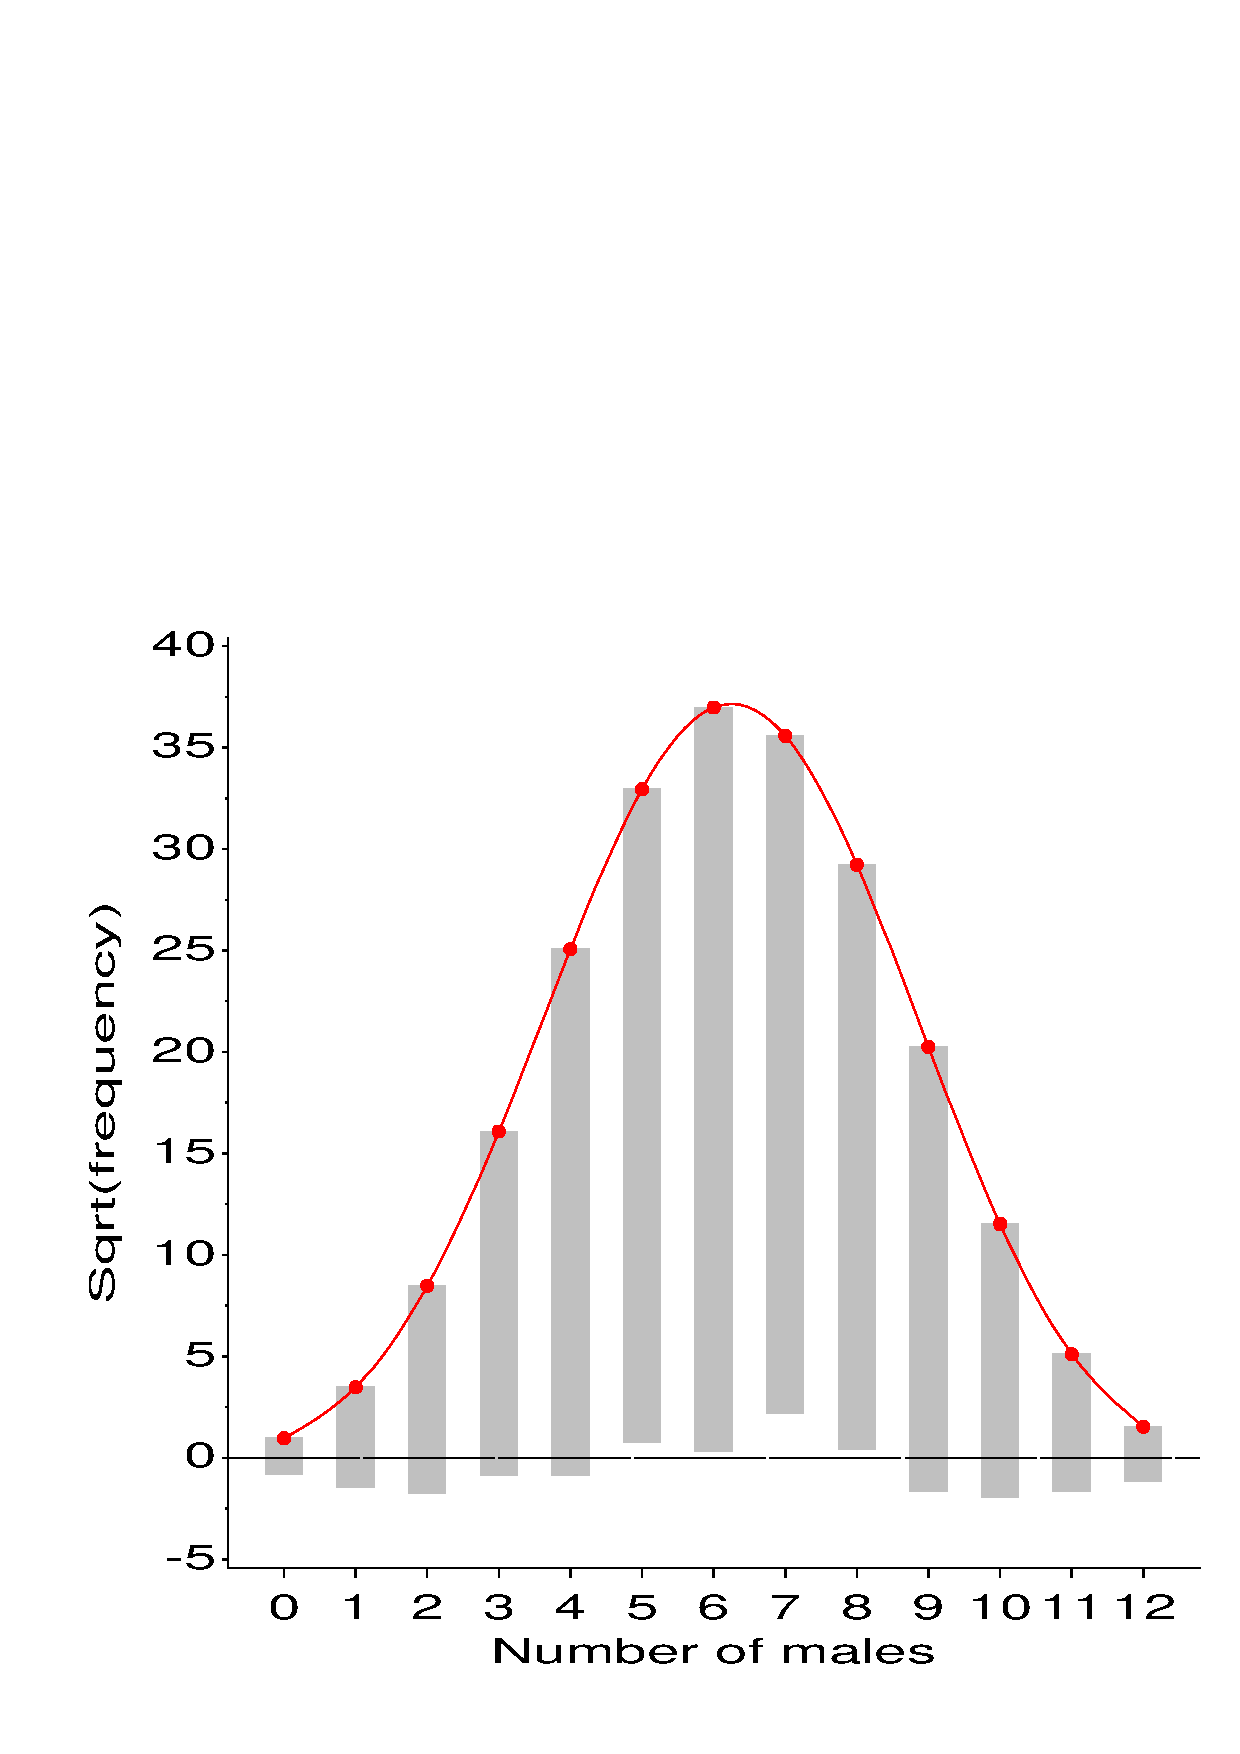
\includegraphics[width=1\linewidth]{saxony}\graphicsfile{ch2/fig/saxony.eps}{}
 \end{minipage}%
 \hfill
 \begin{minipage}[c]{.33\linewidth}
  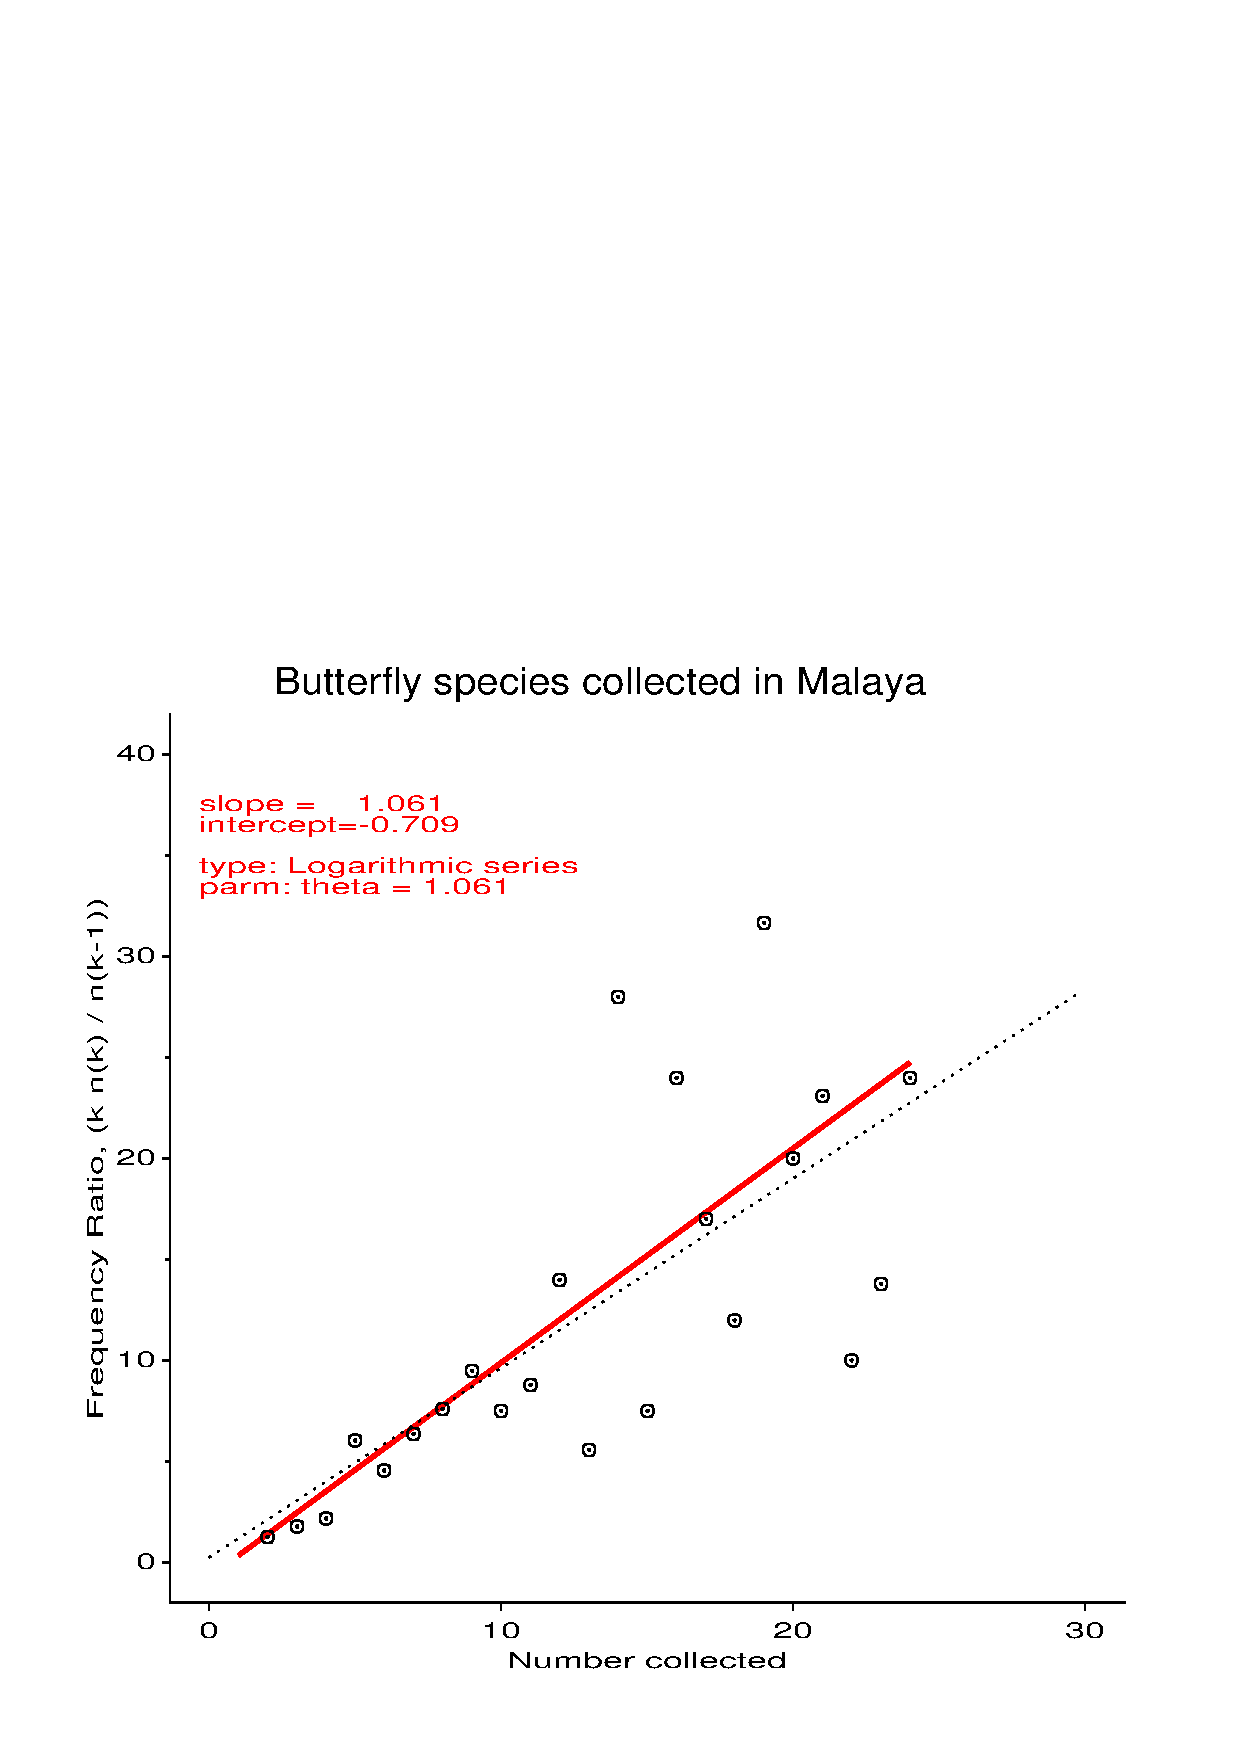
\includegraphics[width=1\linewidth]{orddemo3}\graphicsfile{ch2/fig/orddemo3.eps}{}
 \end{minipage}
 \hfill
 \begin{minipage}[c]{.33\linewidth}
  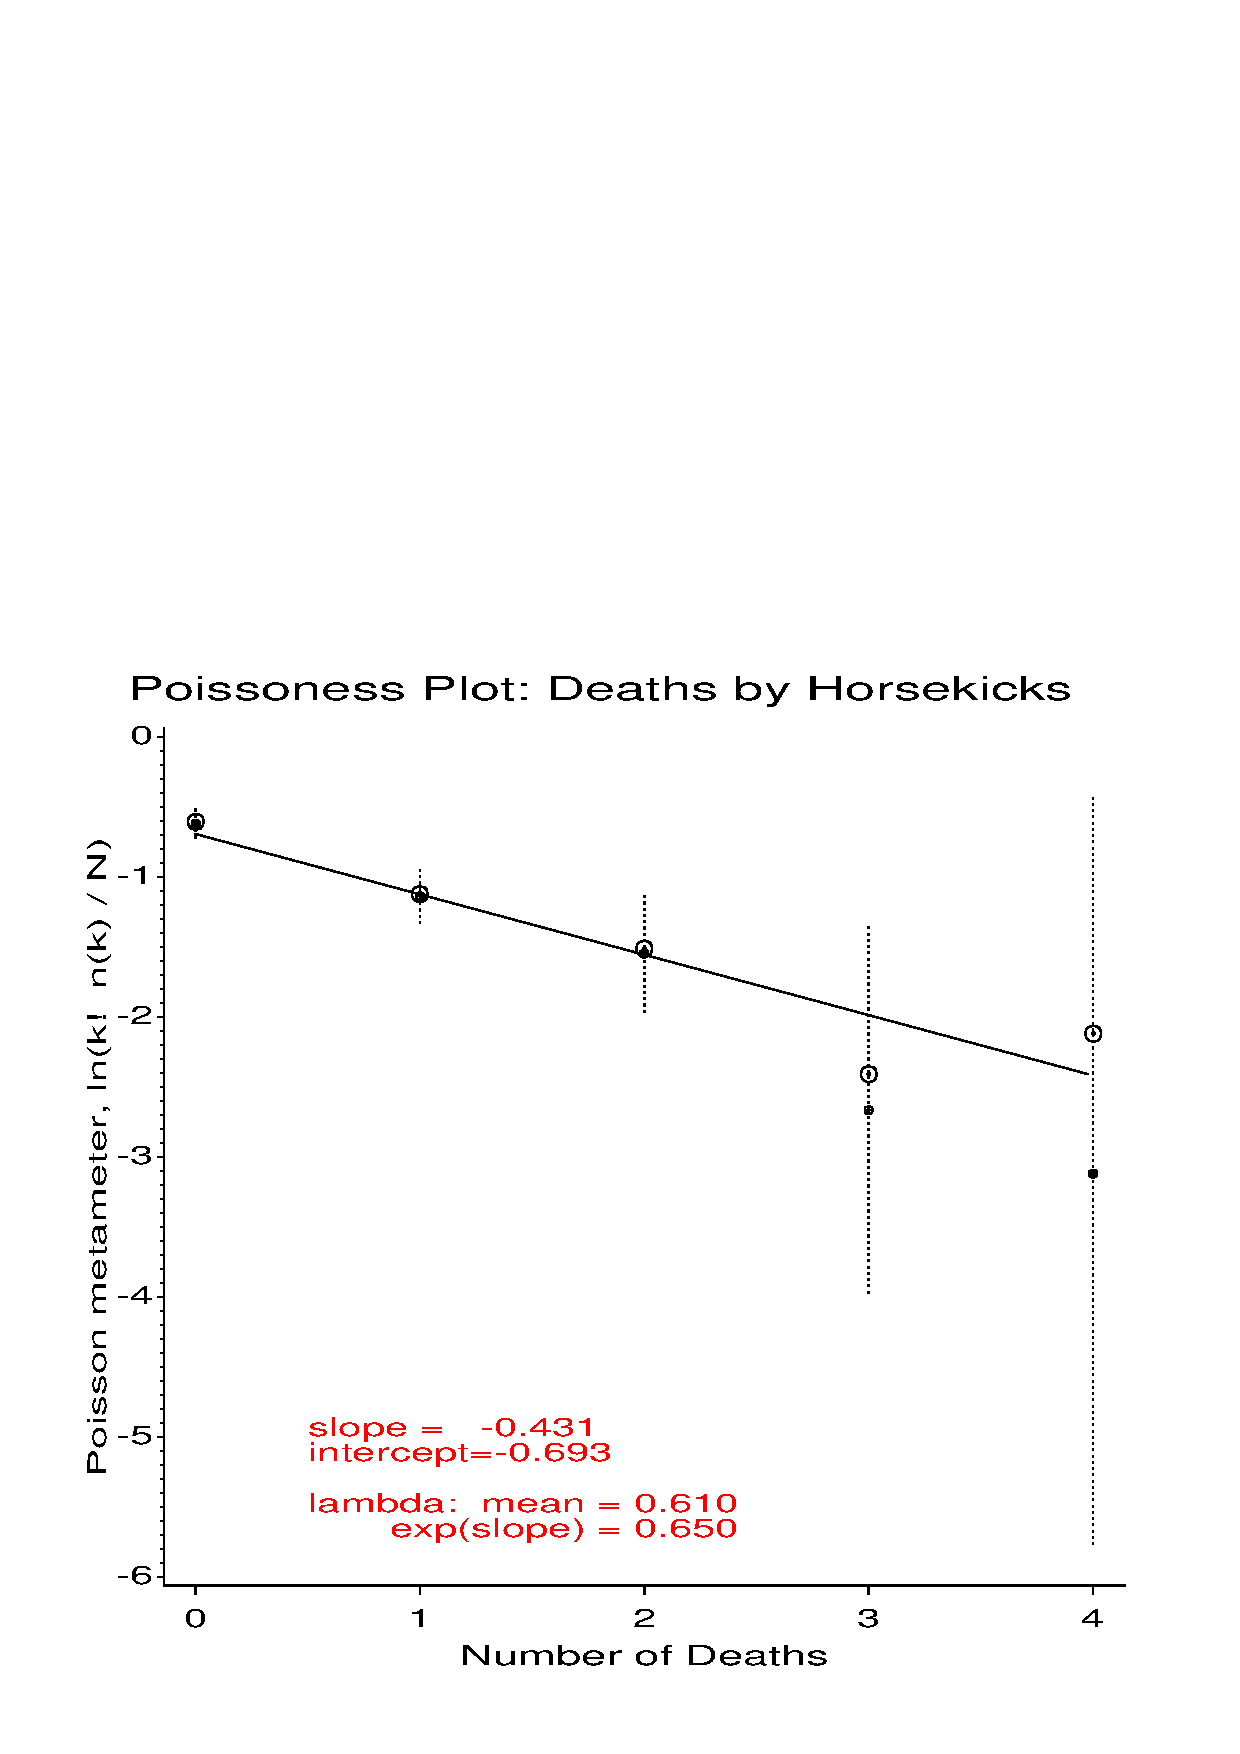
\includegraphics[width=1\linewidth]{poisdemo1}\graphicsfile{ch2/fig/poisdemo1.eps}{}
 \end{minipage}
\end{center}

		% visual table of contents

\chapterprelude{
This chapter introduces the modeling framework for categorical data in the simple
situation where we have a categorical response variable, often binary, and one or
more explanatory variables. A fitted model provides both statistical
inference and prediction, accompanied by measures of uncertainty.
Data visualization methods for discrete response data must often rely
on smoothing techniques, including both direct, non-parametric smoothing
and the implicit smoothing that results from a fitted parametric model.
Diagnostic plots help us to detect influential observations which may distort
our results.
}

% \minitoc
% \clearpage

\section{Introduction}\label{sec:logist-intro}

\epigraph{All models are wrong, but some are useful}{George E. P. Box, \citep[p. 424]{BoxDraper:1987}}
%Reference: Box & Draper (1987), Empirical model-building and response surfaces, Wiley, p. 424.

\chrange{ch:twoway}{ch:corresp}
have been concerned primarily with simple,
exploratory methods for studying the relations among categorical
variables and with testing hypotheses about their associations
through non-parametric tests and with overall goodness-of-fit
statistics.

This chapter begins our study of model-based methods for the analysis
of discrete data.  These models differ from those we have examined
earlier primarily in that they consider \emph{explicitly} an
assumed probability distribution for the observations, and make
clear distinctions between the systematic component, which is
explained by the model, and the random component, which is not.
More importantly, the model-based approach allows a compact summary
of categorical data in terms of a (hopefully) small number of
parameters accompanied by measures of uncertainty (standard errors),
and the ability to estimate predicted values over the range of
explanatory variables.

This model-fitting approach has several advantages:
\begin{seriate}
\item Inferences for the model parameters include both hypothesis tests
and confidence intervals.  
\item The former help us to assess which
explanatory variables affect the outcome;  the size of the estimated
parameters and the widths of their confidence intervals help us to
assess the strength and importance of these effects.
\item There are a variety of methods for model selection, designed
to help determine a favorable trade-off between goodness-of-fit
and parsimony.
\item Finally, the predicted values obtained from the model effectively
smooth the discrete responses, allow predictions for unobserved
values of the explanatory variables, and
provide important means to interpret the fitted relationship graphically.
\end{seriate}

\begin{figure}
 \centering
 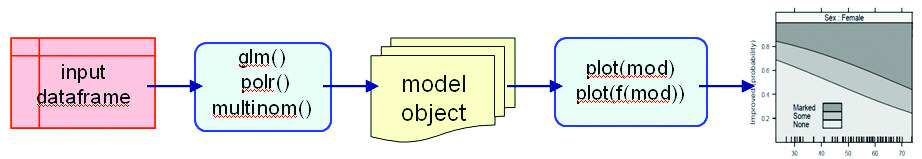
\includegraphics[width=\textwidth]{ch07/fig/goverview-R1}
 \caption{Overview of fitting and graphing for model-based methods in \R.
 }\label{fig:goverview}
\end{figure}

\figref{fig:goverview} provides a visual overview of the steps for fitting and
graphing with model-based methods in \R.  
\begin{seriate}
  \item A modeling function such as
\func{glm} is applied to an input data frame.  The result is a \term{model object}
containing all the information from the fitting process.  
  \item As is standard
in \R, \func{print} and \func{summary} methods give, respectively, basic and
detailed printed output. 
  \item Many modeling functions have \func{plot} methods 
that produce different types of summary and diagnostic plots.  
  \item For visualizing
the fitted model, most model methods provide a \func{predict} method that can
be used to plot the fitted values from the model over the ranges of the
predictors.  Such plots can be customized by the addition of points 
(showing the observations), lines, confidence bands, and so forth.
\end{seriate}

In this chapter we consider models for a \term{binary response},
such as ``success'' or ``failure'',
or the number of ``successes'' in a fixed number of ``trials'',
where we might reasonably assume a binomial distribution for the
random component.  These methods extend readily to
a \term{polytomous response} with more than two outcome categories,
such as improvement in therapy, with categories ``none,'' ``some''
and ``marked.''

These models can be seen as simple extensions of familiar ANOVA and
regression models for quantitative data.  They are also
important special cases of a more general approach, the
\term{generalized linear model} that subsumes a wide variety
of families of techniques within a single, unified framework.
However, rather than starting at the top with the fully
general version, this chapter details the important special
cases of models for discrete outcomes, beginning with binary responses.

This chapter proceeds as follows: in \secref{sec:logist-model}
we introduce the simple logistic regression model for a binary response
and a single quantitative predictor.  This model extends directly
to models for grouped, binomial data (\secref{sec:logist-grouped})
and to models with any number of regressors (\secref{sec:logist-mult}),
which can be quantitative, discrete factors and more general forms.
For interpreting and understanding the results of a fitted model,
we emphasize plotting predicted probabilities and predicted log odds
in various ways, for which effect plots (\secref{sec:logist-effplots})
are particularly useful for complex models.
Individual observations sometimes exert great influence on a fitted model.
Some measures of influence and diagnostic plots are illustrated in
\secref{sec:logist-infl}.
In \secref{sec:logist-poly}, we develop several approaches to
modelling a multi-category (polytomous) response.
%\TODO{Complete this chapter overview.}

\section{The logistic regression model}\label{sec:logist-model}

The logistic regression model
describes the relationship between a discrete outcome variable,
the ``response'', and a set of explanatory variables.
The response variable is often \term{dichotomous}, although
extensions to the model permit multi-category,
\term{polytomous} outcomes, discussed in
\secref{sec:logist-poly}.
The explanatory variables may be continuous or (with factor variables)
discrete.

For a binary response, $Y$, and a continuous explanatory variable, $X$,
we may be interested in modeling the probability of a successful
outcome, which we denote $\pi(x) \equiv \Pr(Y=1 \given X=x)$.
That is, at a given value $X = x$, you can imagine that there is a
binomial distribution of the responses, $\Bin( \pi(x), n_x )$.

The simplest naive model, called the \term{linear probability model},
supposes that this probability, $\pi (x)$ varies
linearly with the value of $x$,
\begin{equation}\label{eq:logit0}
E ( Y \given x) = \pi(x) =
\alpha + \beta x \comma
\end{equation}
where the notation $E ( Y \given x)$ indicates that the probability $\pi (x)$
represents the population
conditional average of the 1s and 0s for all observations with a fixed value of $x$.
For binary observations, this is simply the proportion of 1s.

\figref{fig:arthritis-age} illustrates the basic setup for modeling a binary outcome
using the \data{Arthritis} data, and described more fully in 
\exref{ex:arthrit6}--\exref{ex:arthrit8}.
The 0/1 observations are shown as (jittered) points. 
The predicted values under the linear probability model \eqref{eq:logit0} are shown
as the black line.  As you can see, this model cannot be right, because it predicts
a probability less than 0 for small values of Age, and would also predict
probabilities greater than 1 for larger values of Age.

\begin{figure}[!htb]
\centering
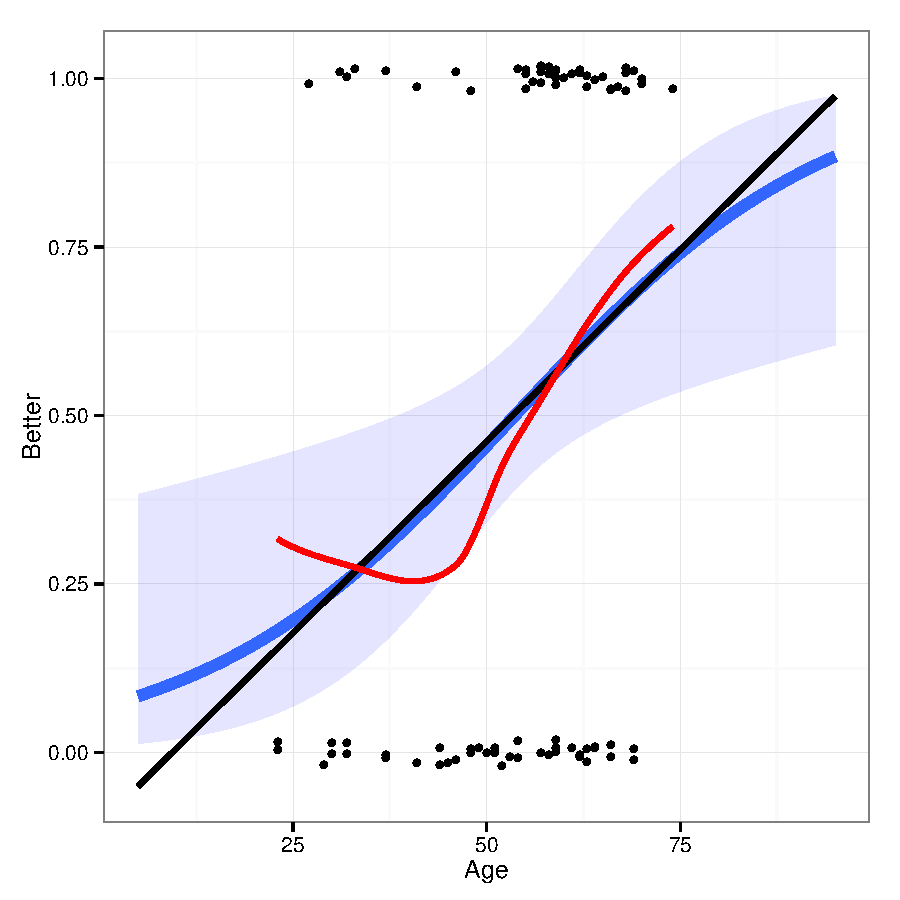
\includegraphics[width=0.7\textwidth]{ch07/fig/arthritis-age}
\caption{Arthritis treatment data, for the relationship of the binary response ``Better'' to Age. The blue curve and shaded confidence band show a fitted logistic regression to the observations shown as jittered points. The black line shows a simple linear regression and the red curve shows a non-parametric (loess) smoothed curve.}
\label{fig:arthritis-age}
\end{figure}

The linear probability model is also wrong because it assumes that the distribution
of residuals, $Y_i - \hat{\pi} (x_i)$ is normal, with mean 0 and constant variance.
However, because $Y$ is dichotomous, the residuals are also dichotomous, and have
variance $\pi (x_i) (1 - \pi (x_i))$, which is maximal for $\pi = 0.5$ and decreases
as $\pi$ goes toward 0 or 1.

One way around the difficulty of needing to constrain the predicted values to
the interval [0, 1]
is to re-specify the model so that a
\emph{transformation} of $\pi$ has a linear relation to $x$, and that transformation
keeps $\hat{\pi}$ between 0 and 1 for all $x$. This idea, of modeling a
transformation of the response that has desired statistical properties is one of
the fundamental ones that led to the development of \term{generalized linear model}s,
which we treat more fully later in \chref{ch:glm}.
%\TODO{Add chref/secref here.}

A particularly convenient choice of the transformation
gives the \term{linear logistic regression model}
(or \term{linear logit model}%
\footnote{
Some writers use the term \emph{logit model} to refer to those using only
categorical predictors; we use the terms logistic regression and
logit regression interchangeably.
}
)
which posits a linear relation between
the \term{log odds} (or \term{logit}) of this probability and $x$,
\begin{equation}\label{eq:logit1}
\logit[ \pi(x) ] \equiv
\log \left( \frac{\pi(x) }{1-\pi(x) } \right) =
\alpha + \beta x \period
\end{equation}
When $\beta > 0$, $\pi (x)$ and the log odds increase as $X$ increases;
when $\beta < 0$ they decrease with $X$.

This model can also be expressed as a model for the probabilities $\pi (x)$
in terms of the \emph{inverse} of the logit transformation used in \eqref{eq:logit1},
\begin{equation}\label{eq:logit1a}
\pi (x) =
\mbox{logit}^{-1}[ \pi(x) ] =
\frac{1}{1 + \exp [- (\alpha + \beta x) ]}
\end{equation}
This transformation uses the cumulative distribution function of
the logistic distribution, $\Lambda (p) = \frac{1}{1+exp(-p)}$,
giving rise to the term \emph{logistic regression}.%
\footnote{
Any other cumulative probability transformation serves the purpose of 
constraining the probabilities to the interval [0, 1].
The cumulative normal transformation $\pi (x) = \Phi (\alpha + \beta x)$
gives the \term{linear probit regression} model.
We don't treat probit models here because:
\begin{seriate}
 \item The logistic and probit models give results so similar that it is
 hard to distinguish them in practice;
 \item The logistic model is simpler to interpret as a linear model for
 the log odds or multiplicative model for the odds.
\end{seriate}
}

From \eqref{eq:logit1} we see that the odds of a success response
can be expressed as
%
\begin{equation}\label{eq:logit2}
\mbox{odds}(Y=1) \equiv \frac{\pi(x) }{1-\pi(x) }  =
\exp (\alpha + \beta x) = e^{\alpha} ( e^{\beta} )^x \comma
\end{equation}
%
which is a multiplicative model for the odds.
So, under the logistic model,
\begin{itemize*}
\item $\beta$ is the change in the log odds associated with a unit
increase in $x$.
The odds are multiplied by $e^{\beta}$ for each unit increase in $x$.
\item $\alpha$ is log odds at $x=0$; $e^{\alpha}$ is the odds of
a favorable response at this $x$-value
(which may not have a reasonable interpretation if $X=0$ is far from
the range of the data).
\end{itemize*}

It is easy to explore the relationships among probabilities, odds and
log odds using \R as we show below, using the function \func{fractions}
in \pkg{MASS} to print the odds corresponding to probability \code{p}
as a fraction.
\begin{knitrout}
\definecolor{shadecolor}{rgb}{1, 0.961, 0.933}\color{fgcolor}\begin{kframe}
\begin{alltt}
\hlkwd{library}\hlstd{(MASS)}
\hlstd{p} \hlkwb{<-} \hlkwd{c}\hlstd{(}\hlnum{.05}\hlstd{,} \hlnum{.10}\hlstd{,} \hlnum{.25}\hlstd{,} \hlnum{.50}\hlstd{,} \hlnum{.75}\hlstd{,} \hlnum{.90}\hlstd{,} \hlnum{.95}\hlstd{)}
\hlkwd{data.frame}\hlstd{(p,}
           \hlkwc{odds}\hlstd{=}\hlkwd{as.character}\hlstd{(}\hlkwd{fractions}\hlstd{(p}\hlopt{/}\hlstd{(}\hlnum{1}\hlopt{-}\hlstd{p))),}
           \hlkwc{logit}\hlstd{=}\hlkwd{log}\hlstd{(p}\hlopt{/}\hlstd{(}\hlnum{1}\hlopt{-}\hlstd{p)))}
\end{alltt}
\begin{verbatim}
##      p odds   logit
## 1 0.05 1/19 -2.9444
## 2 0.10  1/9 -2.1972
## 3 0.25  1/3 -1.0986
## 4 0.50    1  0.0000
## 5 0.75    3  1.0986
## 6 0.90    9  2.1972
## 7 0.95   19  2.9444
\end{verbatim}
\end{kframe}
\end{knitrout}
Thus, a probability of $\pi = 0.25$ represents an odds of 1 to 3, or 1/3,
while a probability of $\pi = 0.75$ represents an odds of 3 to 1, or 3.
The logits are symmetric around 0, so $\logit (.25) = - \logit (.75)$.

Another simple way to interpret the parameter $\beta$ in the logistic regression
model is to consider the relationship between the probability $\pi(x)$ and $x$.
From \eqref{eq:logit1a} it can be shown that the fitted curve
(the blue line in \figref{fig:arthritis-age}) has slope equal to
$\beta\pi (1-\pi)$.  This has a maximum value of $\beta / 4$ when $\pi = \frac12$,
so taking $\beta / 4$ gives a quick estimate of the maximum effect of $x$
on the probability scale.

In \figref{fig:arthritis-age} and other plots later in this chapter we try to show
the binary responses (as jittered points or a rug plot) to help you appreciate how the fitted
logistic curve arises from their distribution across the range a a predictor.
For didactic purposes this can be seen more readily by plotting the conditional distributions
of $x \given y=\{0,1\}$ as a histogram, boxplot or density plot.
The function \func{logi.hist.plot} in the \Rpackage{probio} is a nice implementation of
this idea \citep{Rot:2005}.  The call below produces \figref{fig:arth-logi-hist},
and it is easy to see how increasing age produces a greater probability of a Better
response.


\begin{knitrout}\footnotesize
\definecolor{shadecolor}{rgb}{1, 0.961, 0.933}\color{fgcolor}\begin{kframe}
\begin{alltt}
\hlkwd{with}\hlstd{(Arthritis,}
     \hlkwd{logi.hist.plot}\hlstd{(Age, Better,} \hlkwc{type}\hlstd{=}\hlstr{"hist"}\hlstd{,} \hlkwc{counts}\hlstd{=}\hlnum{TRUE}\hlstd{,}
                    \hlkwc{ylabel}\hlstd{=}\hlstr{"Probability (Better)"}\hlstd{,} \hlkwc{xlab}\hlstd{=}\hlstr{"Age"}\hlstd{,}
                    \hlkwc{col.cur}\hlstd{=}\hlstr{"blue"}\hlstd{,} \hlkwc{col.hist}\hlstd{=}\hlstr{"lightblue"}\hlstd{,} \hlkwc{col.box}\hlstd{=}\hlstr{"lightblue"}\hlstd{)}
  \hlstd{)}
\end{alltt}
\end{kframe}\begin{figure}[!htbp]


\centerline{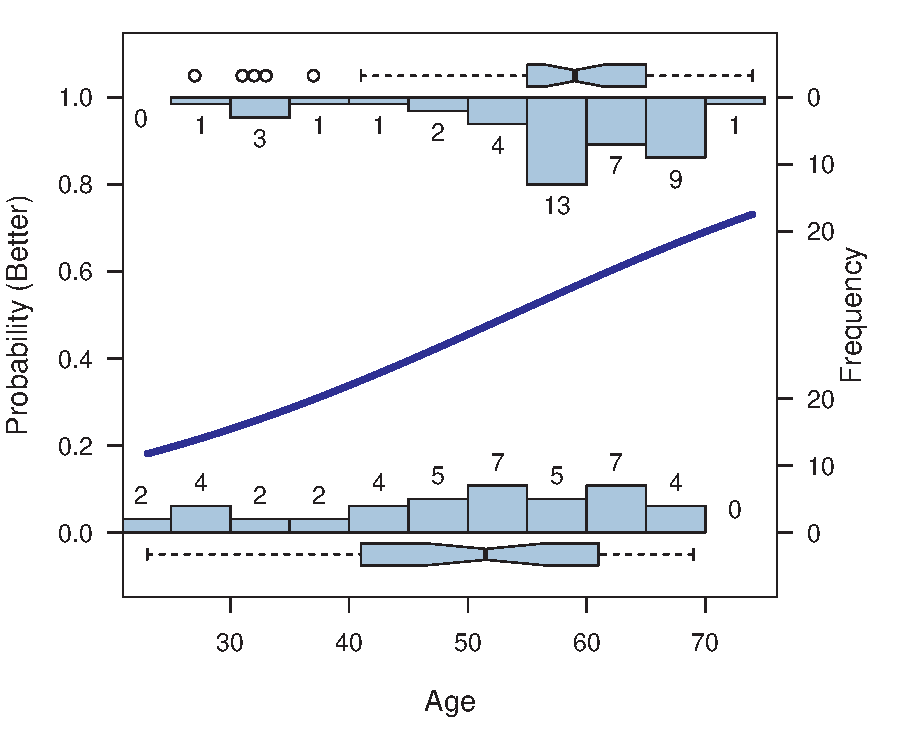
\includegraphics[width=.6\textwidth]{ch07/fig/arth-logi-hist-1} }

\caption[Plot of the Arthritis treatment data, showing the conditional distributions of the 0/1 observations of the Better response by histograms and boxplots]{Plot of the Arthritis treatment data, showing the conditional distributions of the 0/1 observations of the Better response by histograms and boxplots.\label{fig:arth-logi-hist}}
\end{figure}


\end{knitrout}


\subsection{Fitting a logistic regression model}\label{sec:logist-fitting}

Logistic regression models are the special case of generalized linear models
fit in \R using \func{glm} for a binary response using \code{family=binomial}.
We first illustrate how simple models can be fit and interpreted.

\begin{Example}[arthrit6]{Arthritis treatment}
\ixe{Arthritis treatment!logistic regression}

In \chref{ch:twoway} we examined the data
on treatment for rheumatoid arthritis in relation to
two categorical predictors, sex of patient and treatment.
In addition, the \data{Arthritis} data
gives the age of each patient in this study,
and we focus here on the relationship between \var{Age} and the
outcome, \var{Improved}.
This response variable has three categories (none, some, or marked
improvement), but
for now we consider whether the patient showed any
improvement at all, defining the event \code{Better} to be some or
marked improvement.

\begin{knitrout}
\definecolor{shadecolor}{rgb}{1, 0.961, 0.933}\color{fgcolor}\begin{kframe}
\begin{alltt}
\hlkwd{data}\hlstd{(}\hlstr{"Arthritis"}\hlstd{,} \hlkwc{package}\hlstd{=}\hlstr{"vcd"}\hlstd{)}
\hlstd{Arthritis}\hlopt{$}\hlstd{Better} \hlkwb{<-} \hlkwd{as.numeric}\hlstd{(Arthritis}\hlopt{$}\hlstd{Improved} \hlopt{>} \hlstr{"None"}\hlstd{)}
\end{alltt}
\end{kframe}
\end{knitrout}
The logistic regression model is fit using \func{glm} as shown below, specifying
\code{family=binomial} for a binary response.
\begin{knitrout}
\definecolor{shadecolor}{rgb}{1, 0.961, 0.933}\color{fgcolor}\begin{kframe}
\begin{alltt}
\hlstd{arth.logistic} \hlkwb{<-} \hlkwd{glm}\hlstd{(Better} \hlopt{~} \hlstd{Age,} \hlkwc{data}\hlstd{=Arthritis,} \hlkwc{family}\hlstd{=binomial)}
\end{alltt}
\end{kframe}
\end{knitrout}
As usual for \R modeling functions, the \func{print} method for \class{glm} objects gives
brief printed output, while the \func{summary} method is more verbose, and includes
standard errors and hypothesis tests for the model coefficients.  
% To save some space, we define a
% utility function, \func{print\_coef} to extract and print only the table of model coefficients:
To save some space, it is convenient to use the generic function \func{coeftest} from the
\Rpackage{lmtest}.  \TODO{Delete \code{print\_coef} once all uses have been expunged.}

Then, we can use this instead of the more detailed \func{summary}:
\begin{knitrout}
\definecolor{shadecolor}{rgb}{1, 0.961, 0.933}\color{fgcolor}\begin{kframe}
\begin{alltt}
\hlkwd{library}\hlstd{(lmtest)}
\hlkwd{coeftest}\hlstd{(arth.logistic)}
\end{alltt}
\begin{verbatim}
## 
## z test of coefficients:
## 
##             Estimate Std. Error z value Pr(>|z|)  
## (Intercept)  -2.6421     1.0732   -2.46    0.014 *
## Age           0.0492     0.0194    2.54    0.011 *
## ---
## Signif. codes:  0 '***' 0.001 '**' 0.01 '*' 0.05 '.' 0.1 ' ' 1
\end{verbatim}
\end{kframe}
\end{knitrout}


In the output above, the parameter estimates
are $\alpha = -2.642$, and $\beta = 0.0492$.  So, the estimated odds of
a better response are multiplied by $e^{\beta} = \exp(0.0492) = 1.05$
for each one year increase in age.  Equivalently, you can think of this
as a 5\% increase per year (using $100 (e^{\beta} -1)$ to convert).
Over 10 years, the odds are multiplied by $\exp(10 \times 0.0492) = 1.64$,
a 64\% increase, a substantial effect in the range for these data.
You can do these calculations in \R using the \func{coef} method for the \class{glm} object.
\begin{knitrout}
\definecolor{shadecolor}{rgb}{1, 0.961, 0.933}\color{fgcolor}\begin{kframe}
\begin{alltt}
\hlkwd{exp}\hlstd{(}\hlkwd{coef}\hlstd{(arth.logistic))}
\end{alltt}
\begin{verbatim}
## (Intercept)         Age 
##    0.071214    1.050482
\end{verbatim}
\begin{alltt}
\hlkwd{exp}\hlstd{(}\hlnum{10}\hlopt{*}\hlkwd{coef}\hlstd{(arth.logistic)[}\hlnum{2}\hlstd{])}
\end{alltt}
\begin{verbatim}
##    Age 
## 1.6364
\end{verbatim}
\end{kframe}
\end{knitrout}

For comparison with the logistic model, we could fit the linear probability model
\eqref{eq:logit0} using either \func{lm} or \func{glm} with the default
\code{family=gaussian} argument.
\begin{knitrout}
\definecolor{shadecolor}{rgb}{1, 0.961, 0.933}\color{fgcolor}\begin{kframe}
\begin{alltt}
\hlstd{arth.lm} \hlkwb{<-} \hlkwd{glm}\hlstd{(Better} \hlopt{~} \hlstd{Age,} \hlkwc{data}\hlstd{=Arthritis)}
\hlkwd{coef}\hlstd{(arth.lm)}
\end{alltt}
\begin{verbatim}
## (Intercept)         Age 
##   -0.107170    0.011379
\end{verbatim}
\end{kframe}
\end{knitrout}
The coefficient for age can be interpreted to indicate that the probability of a better
response increases by 0.011 for each one year increase in age.  You can compare this
with the $\beta / 4$ rule of thumb, that gives 0.0492/4 = 0.0123.
Even though the linear probability model is inappropriate theoretically, you can
see in \figref{fig:arthritis-age} (the black line)
that it gives similar predicted probabilities to those of the logistic
model between age 25--75, where most of the data points are located.


\end{Example}

\subsection{Model tests for simple logistic regression}\label{sec:logist-tests}

There are two main types of hypothesis tests one might want to perform for a
logistic regression model. We postpone general discussion of this
topic until \secref{sec:logist-mult}, but introduce the main ideas here
using the analysis of the \data{Arthritis} data.
\begin{itemize}
  \item The most basic test answers the
question ``How much better is the fitted model, $\logit(\pi) = \alpha + \beta x$
than the null model $\logit(\pi) = \alpha$ that includes only the
regression intercept?'' One answer to this question is given by the
(Wald) test of the coefficient for age testing the hypothesis $H_0: \beta = 0$
that appeared in the output from
\code{summary(arth.logistic)} shown above. 
The more direct test compares the deviance of the fitted model to the deviance
of the null model, and can be obtained using the \func{anova} function:

% <<>>=
% # vs. null model
% arth.logistic.null <- glm(Better ~ 1, data=Arthritis, family=binomial)
% anova(arth.logistic.null, arth.logistic, test="Chisq")
% @

\begin{knitrout}
\definecolor{shadecolor}{rgb}{1, 0.961, 0.933}\color{fgcolor}\begin{kframe}
\begin{alltt}
\hlkwd{anova}\hlstd{(arth.logistic,} \hlkwc{test}\hlstd{=}\hlstr{"Chisq"}\hlstd{)}
\end{alltt}
\begin{verbatim}
## Analysis of Deviance Table
## 
## Model: binomial, link: logit
## 
## Response: Better
## 
## Terms added sequentially (first to last)
## 
## 
##      Df Deviance Resid. Df Resid. Dev Pr(>Chi)   
## NULL                    83        116            
## Age   1     7.29        82        109    0.007 **
## ---
## Signif. codes:  0 '***' 0.001 '**' 0.01 '*' 0.05 '.' 0.1 ' ' 1
\end{verbatim}
\end{kframe}
\end{knitrout}

  \item A second question is ``How bad is this model, compared to a model
  (the \term{saturated model}) that fits the data perfectly?''  This is a test
  of the size of the residual deviance, that is given by the function
  \func{Summarise} in \pkg{vcdExtra}.
\begin{knitrout}
\definecolor{shadecolor}{rgb}{1, 0.961, 0.933}\color{fgcolor}\begin{kframe}
\begin{alltt}
\hlkwd{Summarise}\hlstd{(arth.logistic)}
\end{alltt}
\begin{verbatim}
## Likelihood summary table:
##               AIC BIC LR Chisq Df Pr(>Chisq)    
## arth.logistic 113 118      109  2     <2e-16 ***
## ---
## Signif. codes:  0 '***' 0.001 '**' 0.01 '*' 0.05 '.' 0.1 ' ' 1
\end{verbatim}
\end{kframe}
\end{knitrout}

The summary of these tests is that linear logistic model \eqref{eq:logit1}
fits significantly better than the null model, but that model also shows
significant lack of fit.
\end{itemize}



\subsection{Plotting a binary response}\label{sec:logist-plotting}

It is often difficult to understand how a binary response can give rise to
a smooth, continuous relation between the predicted response, usually
the probability of an event, and a continuous explanatory variable.
Beyond this, plots of the data together with fitted models 
help you to interpret what these models imply.

We illustrate two approaches below using the \data{Arthritis} data
shown in \figref{fig:arthritis-age}, first using \R base graphics, and
then with the \Rpackage{ggplot2} that makes such graphs somewhat easier to do.

That plot, which was designed for didactic purposes, has the following features:
\begin{itemize*}
  \item It shows the \emph{data}, that is, the 0/1 observations of the \code{Better}
  response in relation to age. To do this effectively and avoid over-plotting, the
  binary responses are jittered.
  \item It plots the predicted (fitted) logistic regression relationship on the scale
  of probability, together with a 95\% confidence band.
  \item It also plots the predicted probabilities from the linear probability model.
  \item A smoothed, non-parametric regression curve for the binary observations
  is also added to the plot to give some indication of possible non-linearity in
  the relationship of Better to age.
\end{itemize*}

\begin{Example}[arthrit7]{Arthritis treatment: Plotting logistic regression with base graphics}
%\ixe{Arthritis treatment!plotting logistic regression}
Here we explain 
how plots similar to \figref{fig:arthritis-age} can be constructed
using \R base graphics. We describe the steps needed to calculate predicted values and confidence
bands and how to add these to a basic plot.  These ideas are the basis for the higher-level
and more convenient plotting methods illustrated later in this chapter.
The steps detailed below give the plot shown in \figref{fig:arthritis-age2}.

% show the plot here, but not the code
\begin{knitrout}
\definecolor{shadecolor}{rgb}{1, 0.961, 0.933}\color{fgcolor}\begin{figure}[!htbp]


\centerline{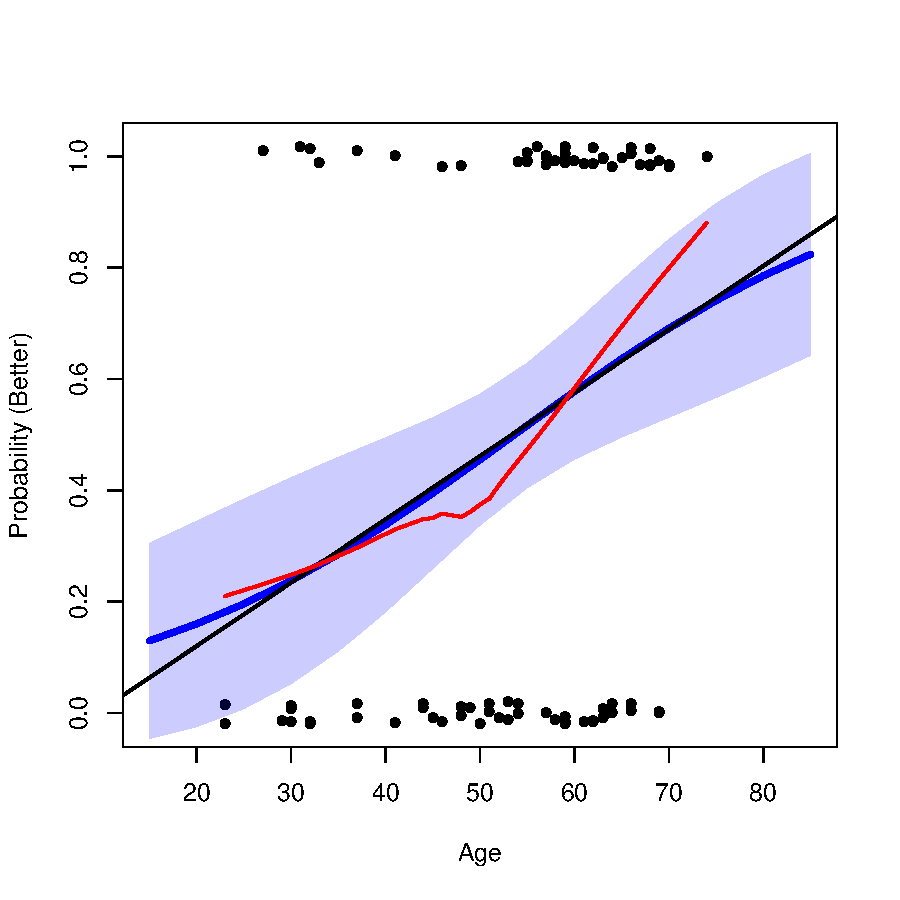
\includegraphics[width=.6\textwidth]{ch07/fig/arthritis-age2-1} }

\caption[A version of plot of the Arthritis treatment data produced with R base graphics]{A version of plot of the Arthritis treatment data (\figref{fig:arthritis-age}) produced with \R base graphics, showing logistic, linear regression and lowess fits.\label{fig:arthritis-age2}}
\end{figure}


\end{knitrout}
First, we set up the basic plot of the jittered values
of \code{Better} vs.\ \code{Age}, setting \code{xlim} to a larger range than
that in the data, only to emphasize where the logistic and linear probability models diverge.

\begin{knitrout}
\definecolor{shadecolor}{rgb}{1, 0.961, 0.933}\color{fgcolor}\begin{kframe}
\begin{alltt}
\hlkwd{plot}\hlstd{(}\hlkwd{jitter}\hlstd{(Better,} \hlnum{.1}\hlstd{)} \hlopt{~} \hlstd{Age,} \hlkwc{data}\hlstd{=Arthritis,}
     \hlkwc{xlim} \hlstd{=} \hlkwd{c}\hlstd{(}\hlnum{15}\hlstd{,}\hlnum{85}\hlstd{),} \hlkwc{pch}\hlstd{=}\hlnum{16}\hlstd{,}
     \hlkwc{ylab}\hlstd{=}\hlstr{"Probability (Better)"}\hlstd{)}
\end{alltt}
\end{kframe}
\end{knitrout}
The fitted logistic curve can be obtained using the \func{predict} method for the
\class{glm} object \code{arth.logistic}.  For this example, we wanted to
get fitted values for the range of Age from 15--85, which is specified
in the \code{newdata} argument.%
\footnote{
Omitting the \code{newdata} argument would give predicted values using the 
linear predictors in the data used for the fitted model.
Some care needs to be taken if the predictor(s) contain missing values.
}
The argument \code{type="response"}
gives fitted values of the probabilities. (The default, \code{type="link"} would
give predicted logits.)  Standard errors of the fitted values are not calculated
by default, so we set \code{se.fit=TRUE}.
\begin{knitrout}
\definecolor{shadecolor}{rgb}{1, 0.961, 0.933}\color{fgcolor}\begin{kframe}
\begin{alltt}
\hlstd{xvalues} \hlkwb{<-} \hlkwd{seq}\hlstd{(}\hlnum{15}\hlstd{,} \hlnum{85}\hlstd{,} \hlnum{5}\hlstd{)}
\hlstd{pred.logistic} \hlkwb{<-} \hlkwd{predict}\hlstd{(arth.logistic,}
                         \hlkwc{newdata}\hlstd{=}\hlkwd{data.frame}\hlstd{(}\hlkwc{Age}\hlstd{=xvalues),}
                         \hlkwc{type}\hlstd{=}\hlstr{"response"}\hlstd{,} \hlkwc{se.fit}\hlstd{=}\hlnum{TRUE}\hlstd{)}
\end{alltt}
\end{kframe}
\end{knitrout}
When \code{se.fit=TRUE},
the \func{predict} function returns its result in a list, with components \code{fit}
for the fitted values and \code{se.fit} for the standard errors.
From these, we can calculate 95\% pointwise prediction intervals
using the standard normal approximation.
\begin{knitrout}
\definecolor{shadecolor}{rgb}{1, 0.961, 0.933}\color{fgcolor}\begin{kframe}
\begin{alltt}
\hlstd{upper} \hlkwb{<-} \hlstd{pred.logistic}\hlopt{$}\hlstd{fit} \hlopt{+} \hlnum{1.96} \hlopt{*} \hlstd{pred.logistic}\hlopt{$}\hlstd{se.fit}
\hlstd{lower} \hlkwb{<-} \hlstd{pred.logistic}\hlopt{$}\hlstd{fit} \hlopt{-} \hlnum{1.96} \hlopt{*} \hlstd{pred.logistic}\hlopt{$}\hlstd{se.fit}
\end{alltt}
\end{kframe}
\end{knitrout}
We can then plot the confidence band using \func{polygon} and the fitted logistic curve
using \code{lines}.  A graphics trick is used here to use a transparent color for
the confidence band using \code{rgb(r, g, b, alpha)}, where \code{alpha} is the
transparency value.
\begin{knitrout}
\definecolor{shadecolor}{rgb}{1, 0.961, 0.933}\color{fgcolor}\begin{kframe}
\begin{alltt}
\hlkwd{polygon}\hlstd{(}\hlkwd{c}\hlstd{(xvalues,} \hlkwd{rev}\hlstd{(xvalues)),}
        \hlkwd{c}\hlstd{(upper,} \hlkwd{rev}\hlstd{(lower)),}
        \hlkwc{col}\hlstd{=}\hlkwd{rgb}\hlstd{(}\hlnum{0}\hlstd{,} \hlnum{0}\hlstd{,} \hlnum{1}\hlstd{,} \hlnum{.2}\hlstd{),} \hlkwc{border}\hlstd{=}\hlnum{NA}\hlstd{)}
\hlkwd{lines}\hlstd{(xvalues, pred.logistic}\hlopt{$}\hlstd{fit,} \hlkwc{lwd}\hlstd{=}\hlnum{4} \hlstd{,} \hlkwc{col}\hlstd{=}\hlstr{"blue"}\hlstd{)}
\end{alltt}
\end{kframe}
\end{knitrout}
This method, using \func{predict} for calculations and \func{polygon} and \func{lines}
for plotting can be used to display the predicted relationships and confidence bands
under other models.  Here, we simply used \func{abline} to plot the fitted line
for the linear probability model \code{arth.lm} and \func{lowess} to calculate
a smoothed, non-parametric curve.

\begin{knitrout}
\definecolor{shadecolor}{rgb}{1, 0.961, 0.933}\color{fgcolor}\begin{kframe}
\begin{alltt}
\hlkwd{abline}\hlstd{(arth.lm,} \hlkwc{lwd}\hlstd{=}\hlnum{2}\hlstd{)}
\hlkwd{lines}\hlstd{(}\hlkwd{lowess}\hlstd{(Arthritis}\hlopt{$}\hlstd{Age, Arthritis}\hlopt{$}\hlstd{Better,} \hlkwc{f}\hlstd{=}\hlnum{.9}\hlstd{),} \hlkwc{col}\hlstd{=}\hlstr{"red"}\hlstd{,} \hlkwc{lwd}\hlstd{=}\hlnum{2}\hlstd{)}
\end{alltt}
\end{kframe}
\end{knitrout}
\end{Example}

\begin{Example}[arthrit8]{Arthritis treatment: Plotting logistic regression with ggplot2}
%\ixe{Arthritis treatment!plotting logistic regression}

Model-based plots such as \figref{fig:arthritis-age} are relatively
more straight-forward to produce using \pkg{ggplot2}. 
The basic steps here are to: 
\begin{itemize*}
  \item set up the plot frame with \func{ggplot} using Age and Better as $(x, y)$ coordinates; 
  \item use \func{geom\_point} to plot the observations,
  whose positions are jittered with \func{position\_jitter};
  \item use \func{stat\_smooth} with \code{method = "glm"} and \code{family = binomial}
  to plot the predicted probability curve and confidence band. By default, \func{stat\_smooth} 
  calculates and plots 95\% confidence bands on the response (probability) scale.
\end{itemize*}

\begin{knitrout}
\definecolor{shadecolor}{rgb}{1, 0.961, 0.933}\color{fgcolor}\begin{kframe}
\begin{alltt}
\hlkwd{library}\hlstd{(ggplot2)}
\hlcom{# basic logistic regression plot}
\hlstd{gg} \hlkwb{<-} \hlkwd{ggplot}\hlstd{(Arthritis,} \hlkwd{aes}\hlstd{(}\hlkwc{x}\hlstd{=Age,} \hlkwc{y}\hlstd{=Better))} \hlopt{+}
  \hlkwd{xlim}\hlstd{(}\hlnum{5}\hlstd{,} \hlnum{95}\hlstd{)} \hlopt{+} \hlkwd{theme_bw}\hlstd{()} \hlopt{+}
  \hlkwd{geom_point}\hlstd{(}\hlkwc{position} \hlstd{=} \hlkwd{position_jitter}\hlstd{(}\hlkwc{height} \hlstd{=} \hlnum{0.02}\hlstd{,} \hlkwc{width} \hlstd{=} \hlnum{0}\hlstd{))} \hlopt{+}
  \hlkwd{stat_smooth}\hlstd{(}\hlkwc{method} \hlstd{=} \hlstr{"glm"}\hlstd{,} \hlkwc{family} \hlstd{= binomial,} \hlkwc{alpha} \hlstd{=} \hlnum{0.1}\hlstd{,} \hlkwc{fill}\hlstd{=}\hlstr{"blue"}\hlstd{,}
              \hlkwc{size}\hlstd{=}\hlnum{2.5}\hlstd{,} \hlkwc{fullrange}\hlstd{=}\hlnum{TRUE}\hlstd{)}
\end{alltt}
\end{kframe}
\end{knitrout}
Finally, we can add other smoothers to the plot, literally by using \code{+} 
to add these to the \class{ggplot} object.
\begin{knitrout}
\definecolor{shadecolor}{rgb}{1, 0.961, 0.933}\color{fgcolor}\begin{kframe}
\begin{alltt}
\hlcom{# add linear model and loess smoothers}
\hlstd{gg} \hlkwb{<-} \hlstd{gg} \hlopt{+} \hlkwd{stat_smooth}\hlstd{(}\hlkwc{method} \hlstd{=} \hlstr{"lm"}\hlstd{,} \hlkwc{se}\hlstd{=}\hlnum{FALSE}\hlstd{,}
                       \hlkwc{size}\hlstd{=}\hlnum{1.2}\hlstd{,} \hlkwc{color}\hlstd{=}\hlstr{"black"}\hlstd{,} \hlkwc{fullrange}\hlstd{=}\hlnum{TRUE}\hlstd{)}
\hlstd{gg} \hlkwb{<-} \hlstd{gg} \hlopt{+} \hlkwd{stat_smooth}\hlstd{(}\hlkwc{method} \hlstd{=} \hlstr{"loess"}\hlstd{,} \hlkwc{se}\hlstd{=}\hlnum{FALSE}\hlstd{,}
                       \hlkwc{span}\hlstd{=}\hlnum{0.95}\hlstd{,} \hlkwc{colour}\hlstd{=}\hlstr{"red"}\hlstd{,} \hlkwc{size}\hlstd{=}\hlnum{1.2}\hlstd{)}
\hlstd{gg}  \hlcom{# show the plot}
\end{alltt}
\end{kframe}
\end{knitrout}

\end{Example}

\subsection{Grouped binomial data}\label{sec:logist-grouped}
A related case occurs with grouped data, where rather than binary observations,
$y_i \in \{0, 1\}$ in case form, 
the data is given in what is called
\term{events/trials form} that 
records the number of successes, $y_i$ that
occurred in $n_i$ trials associated with each setting of the explanatory
variable(s) $x_i$.%
\footnote{
Alternatively, the data may record the number of
successes, $y_i$, and number of failures, $n_i - y_i$.
}
Case form, with binary observations is the special case where $n_i=1$.

Data in events/trials form often arises from \ctab data with a
binary response. For example in the \data{UCBAdmissions} data,
the response variable \var{Admit} with levels \code{"Admitted"},
\code{"Rejected"} could be treated in this way using
the number of applicants as the number of trials.

As before, we can consider $y_i/n_i$ to estimate the probability of success, $\pi_i$
and the distribution of $Y$ to be binomial, $\Bin(\pi_i, n_i)$ at each $x_i$.

In practical applications, there are two main differences between the 
cases of ungrouped, case form data and grouped, event/trials form.

\begin{itemize}

 \item In fitting models using \func{glm}, the model formula, \verb|response ~ terms|, 
 can be given 
 using a \code{response} consisting of a 
 two-column matrix, whose columns contain the numbers of successes $y_i$ 
 and failures $n_i - y_i$.
 Alternatively, the \code{response} can be given as the proportion of successes,
 $y_i / n_i$, but then it is necessary to specify the number of trials as a
 \code{weight}.
 
 \item In plotting the fitted model on the scale of probability, you usually
 have to explicitly plot the fraction of successes, $y_i/n_i$.

\end{itemize}


\begin{Example}[nasa-temp]{Space shuttle disaster}

In \exref{ex:nasa0} and \exref{ex:nasa} we described the background
behind the post-mortem examination of the evidence relating
to the disastrous launch of the space shuttle \emph{Challenger} on January 28, 1986.
Here we consider a simple, but proper analysis of the data
available at the time of launch.  We also use this example to illustrate
some details of the fitting and plotting of grouped binomial data.
As well, we describe some of the possibilities for dealing with
missing data.

The data set \data{SpaceShuttle} in \pkg{vcd} contains
data on the failures of the O-rings in 24 NASA launches
preceding the launch of \emph{Challenger},
as given by \citet{Dalal-etal:89} and \citet{Tufte:97}
also analysed by \citet{Lavine:91}.

Each launch used two booster rockets with a total of
six O-rings, and the data set records as \var{nFailures}
the number of these that were considered damaged after the rockets
were recovered at sea.  In one launch (flight \# 4),
the rocket was lost at sea, so the relevant response variables
are missing.

In this example, we focus on the variable \var{nFailures}
as a binomial with $n_i = 6$ trials. The missing data for
flight 4 can be handled in several ways in the call to
\func{glm}

\begin{knitrout}
\definecolor{shadecolor}{rgb}{1, 0.961, 0.933}\color{fgcolor}\begin{kframe}
\begin{alltt}
\hlkwd{data}\hlstd{(}\hlstr{"SpaceShuttle"}\hlstd{,} \hlkwc{package}\hlstd{=}\hlstr{"vcd"}\hlstd{)}
\hlstd{shuttle.mod} \hlkwb{<-} \hlkwd{glm}\hlstd{(}\hlkwd{cbind}\hlstd{(nFailures,} \hlnum{6} \hlopt{-} \hlstd{nFailures)} \hlopt{~} \hlstd{Temperature,}
          \hlkwc{data} \hlstd{= SpaceShuttle,} \hlkwc{na.action} \hlstd{= na.exclude,}
          \hlkwc{family} \hlstd{= binomial)}
\end{alltt}
\end{kframe}
\end{knitrout}
Alternatively, we can add an explicit \code{trials} variable,
represent the response as the proportion \code{nFailures/trials},
and use \code{weight = trials} to indicate the total number of
observations.
\begin{knitrout}
\definecolor{shadecolor}{rgb}{1, 0.961, 0.933}\color{fgcolor}\begin{kframe}
\begin{alltt}
\hlstd{SpaceShuttle}\hlopt{$}\hlstd{trials} \hlkwb{<-} \hlnum{6}
\hlstd{shuttle.modw} \hlkwb{<-} \hlkwd{glm}\hlstd{(nFailures}\hlopt{/}\hlstd{trials} \hlopt{~} \hlstd{Temperature,} \hlkwc{weight} \hlstd{= trials,}
          \hlkwc{data} \hlstd{= SpaceShuttle,} \hlkwc{na.action} \hlstd{= na.exclude,}
          \hlkwc{family} \hlstd{= binomial)}
\end{alltt}
\end{kframe}
\end{knitrout}
These two approaches give identical results for all practical purposes:
\begin{knitrout}
\definecolor{shadecolor}{rgb}{1, 0.961, 0.933}\color{fgcolor}\begin{kframe}
\begin{alltt}
\hlkwd{all.equal}\hlstd{(}\hlkwd{coef}\hlstd{(shuttle.mod),} \hlkwd{coef}\hlstd{(shuttle.modw))}
\end{alltt}
\begin{verbatim}
## [1] TRUE
\end{verbatim}
\end{kframe}
\end{knitrout}
As before, we can test whether temperature significantly improves prediction
of failure probability using \func{anova}:
\begin{knitrout}
\definecolor{shadecolor}{rgb}{1, 0.961, 0.933}\color{fgcolor}\begin{kframe}
\begin{alltt}
\hlcom{# testing, vs. null model}
\hlkwd{anova}\hlstd{(shuttle.mod,} \hlkwc{test}\hlstd{=}\hlstr{"Chisq"}\hlstd{)}
\end{alltt}
\begin{verbatim}
## Analysis of Deviance Table
## 
## Model: binomial, link: logit
## 
## Response: cbind(nFailures, 6 - nFailures)
## 
## Terms added sequentially (first to last)
## 
## 
##             Df Deviance Resid. Df Resid. Dev Pr(>Chi)  
## NULL                           22       24.2           
## Temperature  1     6.14        21       18.1    0.013 *
## ---
## Signif. codes:  0 '***' 0.001 '**' 0.01 '*' 0.05 '.' 0.1 ' ' 1
\end{verbatim}
\end{kframe}
\end{knitrout}

The code below gives a \pkg{ggplot2} version in \figref{fig:nasa-temp-ggplot}
of the plot we showed earlier in \exref{ex:nasa0} (\figref{fig:spaceshuttle0}).
The relevant details here are:
\begin{itemize*}
  \item We specify \code{y = nFailures / trials} to calculate the failure probabilities.
  \item Points are jittered in the call to \func{geom\_point} to prevent overplotting.
  \item In the call to \func{geom\_smooth}, we need to use \code{weight = trials},
  just as in the call to \func{glm} above.
  \item \code{fullrange = TRUE} makes the fitted regression curve and
  confidence band extend across the entire plot
\end{itemize*}
%% Running this gives an error under RStudio, but not in the R console
\begin{knitrout}
\definecolor{shadecolor}{rgb}{1, 0.961, 0.933}\color{fgcolor}\begin{kframe}
\begin{alltt}
\hlkwd{library}\hlstd{(ggplot2)}
\hlkwd{ggplot}\hlstd{(SpaceShuttle,} \hlkwd{aes}\hlstd{(}\hlkwc{x} \hlstd{= Temperature,} \hlkwc{y} \hlstd{= nFailures} \hlopt{/} \hlstd{trials))} \hlopt{+}
  \hlkwd{xlim}\hlstd{(}\hlnum{30}\hlstd{,} \hlnum{81}\hlstd{)} \hlopt{+} \hlkwd{theme_bw}\hlstd{()} \hlopt{+}
  \hlkwd{xlab}\hlstd{(}\hlstr{"Temperature (F)"}\hlstd{)} \hlopt{+}
  \hlkwd{ylab}\hlstd{(}\hlstr{"O-Ring Failure Probability"}\hlstd{)} \hlopt{+}
  \hlkwd{geom_point}\hlstd{(}\hlkwc{position}\hlstd{=}\hlkwd{position_jitter}\hlstd{(}\hlkwc{width}\hlstd{=}\hlnum{0}\hlstd{,} \hlkwc{height}\hlstd{=}\hlnum{0.01}\hlstd{),}
             \hlkwd{aes}\hlstd{(}\hlkwc{size} \hlstd{=} \hlnum{2}\hlstd{))} \hlopt{+}
  \hlkwd{theme}\hlstd{(}\hlkwc{legend.position}\hlstd{=}\hlstr{"none"}\hlstd{)} \hlopt{+}
  \hlkwd{geom_smooth}\hlstd{(}\hlkwc{method} \hlstd{=} \hlstr{"glm"}\hlstd{,} \hlkwc{family} \hlstd{= binomial,} \hlkwc{fill}\hlstd{=}\hlstr{"blue"}\hlstd{,}
              \hlkwd{aes}\hlstd{(}\hlkwc{weight} \hlstd{= trials),} \hlkwc{fullrange} \hlstd{=} \hlnum{TRUE}\hlstd{,} \hlkwc{alpha}\hlstd{=}\hlnum{0.2}\hlstd{,} \hlkwc{size}\hlstd{=}\hlnum{2}\hlstd{)}
\end{alltt}
\end{kframe}
\end{knitrout}

\begin{figure}
\centering
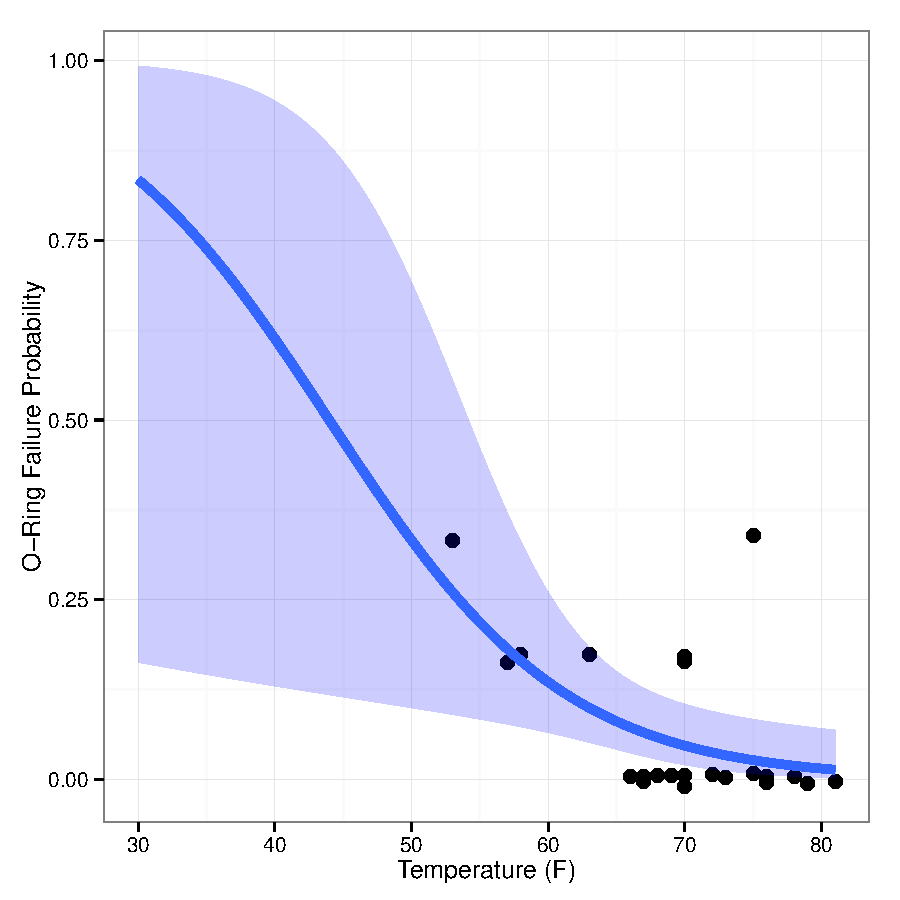
\includegraphics[width=.7\textwidth]{ch07/fig/nasa-temp-ggplot}
\caption{Space shuttle data, with fitted logistic regression model}
\label{fig:nasa-temp-ggplot}
\end{figure}

\end{Example}

%\section{Models for quantitative predictors}\label{sec:logist-quant}

%\section{Logit models for qualitative predictors}\label{sec:logist-qual}

\section{Multiple logistic regression models}\label{sec:logist-mult}

As is the case in classical regression, generalizing the simple logistic
regression to an arbitrary number of explanatory variables is quite straightforward.
We let $\vec{x}_{i} = ( x_{i1}, x_{i2}, \dots , x_{ip})$ denote the vector
of $p$ explanatory variables for case or cluster $i$. Then the general logistic
regression model can be expressed as
\begin{eqnarray}
  \logit ( \pi_{i}) \equiv \log \frac{\pi_i}{1-\pi_i}
   &=& \alpha + \vec{x}_{i}\trans \,  \vec{\beta} \\ \label{eq:logistm1}
   &=& \alpha + \beta_1 x_{i1} + \beta_2 x_{i2} + \cdots + \beta_p x_{ip} \period
   \nonumber
\end{eqnarray}
Equivalently, we can represent this model in terms of probabilities as the
logistic transformation of the \term{linear predictor}, 
$\eta_i =  \alpha + \vec{x}_{i}\trans \,  \vec{\beta} $,
\begin{eqnarray}
   \pi_{i} = \Lambda (\eta_i) 
   &=& \Lambda (\alpha + \vec{x}_{i}\trans \,  \vec{\beta} ) \\ \label{eq:logistm2}
   &=& \frac{1}{1+ \exp(\alpha + \beta_1 x_{i1} + \beta_2 x_{i2} + \cdots + \beta_p x_{ip})} \period
   \nonumber
\end{eqnarray}

The $x$s can include any of the following sorts of regressors,
as in the general linear model:
\begin{itemize*}
\item \textbf{quantitative} variables (e.g., age, income)
\item \textbf{polynomial} powers of quantitative variables (e.g., age, age$^2$, age$^3$)
\item \textbf{transformations} of quantitative variables (e.g., log salary)
\item factors, represented as \textbf{dummy} variables for qualitative predictors (e.g.,
$P_1, P_2, P_3$ for four political party affiliations)
\item \textbf{interaction} terms (e.g., sex $\times$ age, or age $\times$ income)
\end{itemize*}

\begin{Example}[arthrit-mult]{Arthritis treatment}
We continue with the analysis of the \data{Arthritis} data,
fitting a model containing the main effects of \var{Age}, \var{Sex} and \var{Treatment},
with \var{Better} as the response. This model has the form 
\begin{equation*}
  \logit ( \pi_{i}) = \alpha + \beta_1 x_{i1} + \beta_2 x_{i2} + \beta_2 x_{i2}
\end{equation*}
where $x_1$ is \var{Age} and $x_2$ and $x_3$ are the factors 
representing \var{Sex} and \var{Treatment}, respectively.
Using the default (0/1) dummy coding that \R uses (``treatment'' contrasts against the lowest
factor level),%
\footnote{
For factor variables with the default treatment contrasts, you can change the
reference level using \func{relevel}.  In this example, you could make 
male the baseline category using
\code{Arthritis\$Sex <- relevel(Arthritis\$Sex, ref = "Male")}.
}
they are defined as: 
\begin{equation*}
 x_2 = \left\{
    \begin{array}{ll}
    0  & \mbox{ if Female} \\
    1  & \mbox{ if Male} 
    \end{array}
    \right.
 \qquad\qquad
 x_3 = \left\{
    \begin{array}{ll}
    0  & \mbox{ if Placebo} \\
    1  & \mbox{ if Treatment}
    \end{array}
    \right.
\end{equation*}
In this model,
\begin{itemize}
\item $\alpha$ doesn't have a sensible interpretation here, but formally it would be
the log odds of improvement for a person at age $x_1=0$ in
the baseline or reference group
with $x_2=0$ and $x_3=0$---females receiving the placebo.  To make the intercept
interpretable, we will fit the model centering age near the mean,
by using $x_1 - 50$ as the first regressor.

\item \(\beta_1\) is the increment in log odds of improvement for each one-year
increase in age.
\item \(\beta_2\) is the increment in log odds for male
as compared to female.
Therefore, \(e^{ \beta_2 }\) gives the odds of improvement
for males relative to females.

\item \(\beta_3\) is the increment in log odds for being in the
treated group.  \(e^{ \beta_2 }\) gives the odds of
improvement for the active treatment group relative to
placebo.
\end{itemize}

We fit the model as follows.  In \func{glm} model formulas, ``\code{-}'' has a special meaning, so we use
the identity function, \code{I(Age-50)} to center age.
\begin{knitrout}
\definecolor{shadecolor}{rgb}{1, 0.961, 0.933}\color{fgcolor}\begin{kframe}
\begin{alltt}
\hlstd{arth.logistic2} \hlkwb{<-} \hlkwd{glm}\hlstd{(Better} \hlopt{~} \hlkwd{I}\hlstd{(Age}\hlopt{-}\hlnum{50}\hlstd{)} \hlopt{+} \hlstd{Sex} \hlopt{+} \hlstd{Treatment,}
                      \hlkwc{data}\hlstd{=Arthritis,}
                      \hlkwc{family}\hlstd{=binomial)}
\end{alltt}
\end{kframe}
\end{knitrout}


The parameters defined here are \emph{incremental effects}.  The
intercept corresponds to a baseline group (50 year-old females given the placebo);
the other parameters are incremental effects for the other groups
compared to the baseline group.
Thus, when \(\alpha\), \(\beta _1\), \(\beta _2\) and \(\beta _3\)  have
been estimated, the fitted logits and predicted odds at \code{Age==50} are:

\begin{center}
\vspace{1ex}
{\renewcommand{\arraystretch}{1.2}
\begin{tabular}{|ll|cc|}
\hline
Sex  &  Treatment & Logit & Odds Improved  \\[.5ex] \hline

Female  & Placebo  & \(\alpha \) & \(e^{\alpha}\) \\
Female   & Treated  & \(\alpha + \beta_2 \) & \(e^{\alpha + \beta_2 }\) \\
Male & Placebo & \(\alpha + \beta_1 \) & \(e^{\alpha + \beta_1 }\) \\
Male & Treated & \(\alpha + \beta_1 + \beta_2\) & \(e^{\alpha + \beta_1 + \beta_2}\)  \\  \hline
\end{tabular}
}
\end{center}

We first focus on the interpretation of the coefficients estimated for this model
shown below.
\begin{knitrout}
\definecolor{shadecolor}{rgb}{1, 0.961, 0.933}\color{fgcolor}\begin{kframe}
\begin{alltt}
\hlkwd{coeftest}\hlstd{(arth.logistic2)}
\end{alltt}
\begin{verbatim}
## 
## z test of coefficients:
## 
##                  Estimate Std. Error z value Pr(>|z|)   
## (Intercept)       -0.5781     0.3674   -1.57    0.116   
## I(Age - 50)        0.0487     0.0207    2.36    0.018 * 
## SexMale           -1.4878     0.5948   -2.50    0.012 * 
## TreatmentTreated   1.7598     0.5365    3.28    0.001 **
## ---
## Signif. codes:  0 '***' 0.001 '**' 0.01 '*' 0.05 '.' 0.1 ' ' 1
\end{verbatim}
\end{kframe}
\end{knitrout}
To interpret these in terms of odds ratios and also find confidence intervals,
just use \func{exp} and \func{confint}.
\begin{knitrout}
\definecolor{shadecolor}{rgb}{1, 0.961, 0.933}\color{fgcolor}\begin{kframe}
\begin{alltt}
\hlkwd{exp}\hlstd{(}\hlkwd{cbind}\hlstd{(}\hlkwc{OddsRatio}\hlstd{=}\hlkwd{coef}\hlstd{(arth.logistic2),}
          \hlkwd{confint}\hlstd{(arth.logistic2)))}
\end{alltt}
\begin{verbatim}
##                  OddsRatio    2.5 %   97.5 %
## (Intercept)        0.56094 0.264749  1.13234
## I(Age - 50)        1.04995 1.010001  1.09630
## SexMale            0.22586 0.065238  0.68908
## TreatmentTreated   5.81130 2.118702 17.72658
\end{verbatim}
\end{kframe}
\end{knitrout}
Here,
\begin{itemize*}
  \item $\alpha = -0.578$: At age 50, females given the placebo have an odds of improvement
  of  $\exp{-0.578} = 0.56$.
  \item $\beta_1 = 0.0487$: Each year of age multiplies the odds of improvement by
  $\exp(0.0487) = 1.05$, or a 5\% increase.
  \item $\beta_2 = -1.49$: Males are only $\exp(-1.49) = 0.26$ times as likely to show
  improvement relative to females.  Equivalently, you could say that females are
  $\exp(1.49) = 4.437$ times more likely than males to improve.
  \item $\beta_3 = 1.76$: People given the active treatment are $\exp(1.76) = 5.8$
  times more likely to show improvement.
\end{itemize*}

As you can see, the interpretation of coefficients in multiple logistic models
is straightforward, though a bit cumbersome.  This becomes more difficult in
larger models, particularly when there are interactions.  In these cases, 
you can understand (and explain) a fitted model more easily through plots of
predicted values, either on the scale of response probability or on the logit
scale of the linear predictor.  We describe these methods in 
\secref{sec:logist-condplots}--\secref{sec:logist-effplots} below.

 
\end{Example}

\subsection{Conditional plots}\label{sec:logist-condplots}
The simplest kind of plots display the data together with a representation
of the fitted relationship (predicted values, confidence bands) 
separately for subsets of the data defined by one or more of the predictors.
Such plots can show the predicted values for the response variable on the ordinate
against one chosen predictor on the abscissa, and can use multiple curves
and multiple panels to represent other predictors.

However, these plots are \term{conditional plots}, meaning that the data 
shown in each panel and used in each fitted curve are limited to the subset
of the observations defined by the curve and panel variables.  As well, 
predictors that are not shown in a given plot are effectively ignored
(or marginalized), as was the case in \figref{fig:arthritis-age}
that showed only the effect of age in the \data{Arthritis} data.

\begin{Example}[arth-cond]{Arthritis treatment: conditional plots}

For the \data{Arthritis} data, a basic conditional plot of \var{Better} vs.\ \var{Age},
showing the observations as jittered points (with \func{geom\_point})
and the fitted logistic curves (with \func{stat\_smooth} using \code{method="glm"})
can be produced with \pkg{ggplot2} as shown below, giving \figref{fig:arth-cond1}.
\begin{knitrout}
\definecolor{shadecolor}{rgb}{1, 0.961, 0.933}\color{fgcolor}\begin{kframe}
\begin{alltt}
\hlkwd{library}\hlstd{(ggplot2)}
\hlstd{gg} \hlkwb{<-} \hlkwd{ggplot}\hlstd{(Arthritis,} \hlkwd{aes}\hlstd{(Age, Better,} \hlkwc{color}\hlstd{=Treatment))} \hlopt{+}
  \hlkwd{xlim}\hlstd{(}\hlnum{5}\hlstd{,} \hlnum{95}\hlstd{)} \hlopt{+} \hlkwd{theme_bw}\hlstd{()} \hlopt{+}
  \hlkwd{geom_point}\hlstd{(}\hlkwc{position} \hlstd{=} \hlkwd{position_jitter}\hlstd{(}\hlkwc{height} \hlstd{=} \hlnum{0.02}\hlstd{,} \hlkwc{width} \hlstd{=} \hlnum{0}\hlstd{))} \hlopt{+}
  \hlkwd{stat_smooth}\hlstd{(}\hlkwc{method} \hlstd{=} \hlstr{"glm"}\hlstd{,} \hlkwc{family} \hlstd{= binomial,} \hlkwc{alpha} \hlstd{=} \hlnum{0.2}\hlstd{,}
              \hlkwd{aes}\hlstd{(}\hlkwc{fill}\hlstd{=Treatment),} \hlkwc{size}\hlstd{=}\hlnum{2.5}\hlstd{,} \hlkwc{fullrange}\hlstd{=}\hlnum{TRUE}\hlstd{)}
\hlstd{gg}   \hlcom{# show the plot}
\end{alltt}
\end{kframe}\begin{figure}[!htbp]


\centerline{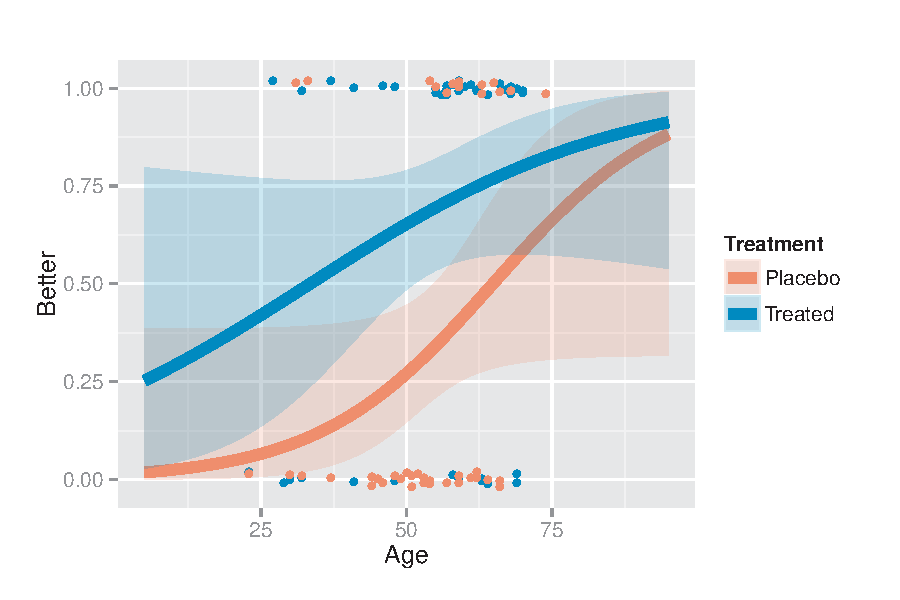
\includegraphics[width=.6\textwidth]{ch07/fig/arth-cond1-1} }

\caption[Conditional plot of Arthritis data showing separate points and fitted curves stratified by Treatment]{Conditional plot of Arthritis data showing separate points and fitted curves stratified by Treatment. A separate fitted curve is shown for the two treatment conditions, ignoring Sex.\label{fig:arth-cond1}}
\end{figure}


\end{knitrout}
\noindent In this call to \func{ggplot},
specifying \code{color=Treatment} gives different point and line colors, but also
automatically stratifies the fitted curves using the levels of this variable.

With such a plot, it is easy to add further stratifying variables in the data
using \term{facets} to produce separate panels (functions \func{facet\_wrap} or \func{facet\_grid}, with
different options to control the details).  The following line further stratifies
by \var{Sex}, producing \figref{fig:arth-cond2}.

\begin{knitrout}
\definecolor{shadecolor}{rgb}{1, 0.961, 0.933}\color{fgcolor}\begin{kframe}
\begin{alltt}
\hlstd{gg} \hlopt{+} \hlkwd{facet_wrap}\hlstd{(}\hlopt{~} \hlstd{Sex)}
\end{alltt}
\end{kframe}\begin{figure}[!htbp]


\centerline{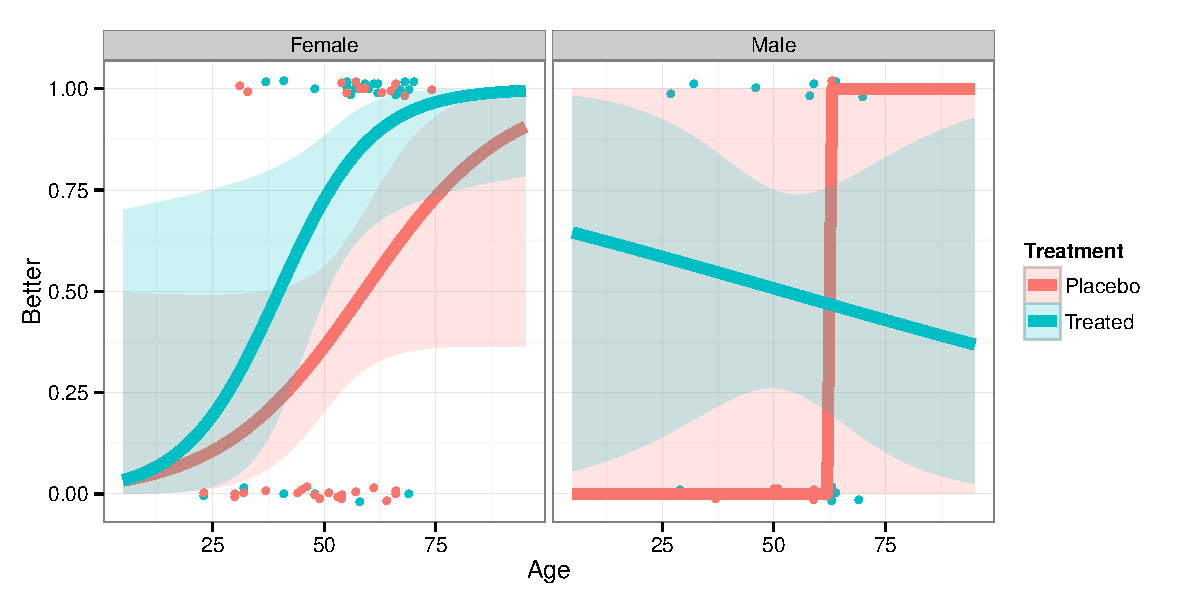
\includegraphics[width=.8\textwidth,clip]{ch07/fig/arth-cond2-1} }

\caption[Conditional plot of Arthritis data, stratified by Treatment and Sex]{Conditional plot of Arthritis data, stratified by Treatment and Sex. The unusual patterns in the panel for Males signals a problem with this data.\label{fig:arth-cond2}}
\end{figure}


\end{knitrout}
\noindent However, you can see from this plot how this method breaks down when the sample size is small in some of the groups defined by  the stratifying factors. The panel for males shows a
paradoxical negative relation with age for the treated group and a step function for the 
placebo group.  The explanation for this is shown in the two-way frequency table
of the sex and treatment combinations:
\begin{knitrout}
\definecolor{shadecolor}{rgb}{1, 0.961, 0.933}\color{fgcolor}\begin{kframe}
\begin{alltt}
\hlkwd{addmargins}\hlstd{(}\hlkwd{xtabs}\hlstd{(}\hlopt{~}\hlstd{Sex} \hlopt{+} \hlstd{Treatment,} \hlkwc{data}\hlstd{=Arthritis),} \hlnum{2}\hlstd{)}
\end{alltt}
\begin{verbatim}
##         Treatment
## Sex      Placebo Treated Sum
##   Female      32      27  59
##   Male        11      14  25
\end{verbatim}
\end{kframe}
\end{knitrout}
Less than 1/3 of the sample were males, and of these only 11 were in the placebo group.
\func{glm} cannot estimate the fitted relationship against \var{Age} here--- the slope
coefficient is infinite, and the fitted probabilities are all either 0 or 1.%
\footnote{
This is called \term{complete separation},  and occurs whenever the responses have no
overlap on the predictor variable(s) used in fitting the logistic regression model.
}

\end{Example}


\subsection{Full-model plots}\label{sec:logist-fullplots}
For a model with two or more explanatory variables, \emph{full-model plots}
display the fitted response surface for all predictors together, rather than
stratified by conditioning variables.
Such plots show the predicted values for the response variable on the ordinate
against one chosen predictor on the abscissa, and can use multiple curves
and multiple panels to represent other predictors.

A simple \R trick%
\footnote{Thanks to Dennis Murphy for suggesting this method.}
makes this method far easier and more general than the naive plotting method
used in \exref{ex:arthrit7}.  The trick is simply to combine the columns in the
original data frame with the result of the \func{predict} method for the fitted model
and plot the calculated \code{fit} value, together with confidence bands
(if you use \code{se.fit=TRUE}).

\begin{Example}[arth-full]{Arthritis treatment: full-model plots}
\begin{knitrout}
\definecolor{shadecolor}{rgb}{1, 0.961, 0.933}\color{fgcolor}\begin{kframe}
\begin{alltt}
\hlstd{arth.fit2} \hlkwb{<-} \hlkwd{cbind}\hlstd{(Arthritis,}
                  \hlkwd{predict}\hlstd{(arth.logistic2,} \hlkwc{se.fit} \hlstd{=} \hlnum{TRUE}\hlstd{))}
\end{alltt}
\end{kframe}
\end{knitrout}
The fitted values here are on the logit scale, which means that it takes one more
trick to show the data points on the plot.  We simply define a new variable,
\code{obs} with convenient logit values corresponding the \code{Better} values
of 0 and 1.
\begin{knitrout}
\definecolor{shadecolor}{rgb}{1, 0.961, 0.933}\color{fgcolor}\begin{kframe}
\begin{alltt}
\hlstd{arth.fit2}\hlopt{$}\hlstd{obs} \hlkwb{<-} \hlkwd{c}\hlstd{(}\hlopt{-}\hlnum{4}\hlstd{,} \hlnum{4}\hlstd{)[}\hlnum{1}\hlopt{+}\hlstd{arth.fit2}\hlopt{$}\hlstd{Better]}
\end{alltt}
\end{kframe}
\end{knitrout}

We can then plot the fitted logit against \var{Age} using \code{x=Age, y=fit}
from the data frame containing the fitted values.  The call to \func{ggplot}
below produces \figref{fig:arth-full1}.  Here, we used \code{color=Treatment}
to produce separate points, lines and confidence bands colored by \var{Treatment}.
Confidence bands in the plot are constructed using \func{geom\_ribbon}.
\begin{knitrout}
\definecolor{shadecolor}{rgb}{1, 0.961, 0.933}\color{fgcolor}\begin{kframe}
\begin{alltt}
\hlkwd{ggplot}\hlstd{(arth.fit2,} \hlkwd{aes}\hlstd{(}\hlkwc{x}\hlstd{=Age,} \hlkwc{y}\hlstd{=fit,} \hlkwc{color}\hlstd{=Treatment))} \hlopt{+}
  \hlkwd{geom_line}\hlstd{(}\hlkwc{size} \hlstd{=} \hlnum{2}\hlstd{)} \hlopt{+} \hlkwd{theme_bw}\hlstd{()} \hlopt{+}
  \hlkwd{geom_ribbon}\hlstd{(}\hlkwd{aes}\hlstd{(}\hlkwc{ymin} \hlstd{= fit} \hlopt{-} \hlnum{1.96} \hlopt{*} \hlstd{se.fit,}
                  \hlkwc{ymax} \hlstd{= fit} \hlopt{+} \hlnum{1.96} \hlopt{*} \hlstd{se.fit,}
                  \hlkwc{fill} \hlstd{= Treatment),} \hlkwc{alpha} \hlstd{=} \hlnum{0.2}\hlstd{,}
              \hlkwc{color} \hlstd{=} \hlstr{"transparent"}\hlstd{)} \hlopt{+}
  \hlkwd{labs}\hlstd{(}\hlkwc{x} \hlstd{=} \hlstr{"Age"}\hlstd{,} \hlkwc{y} \hlstd{=} \hlstr{"Log odds (Better)"}\hlstd{)} \hlopt{+}
  \hlkwd{geom_point}\hlstd{(}\hlkwd{aes}\hlstd{(}\hlkwc{y}\hlstd{=obs),}
             \hlkwc{position}\hlstd{=}\hlkwd{position_jitter}\hlstd{(}\hlkwc{height}\hlstd{=}\hlnum{0.25}\hlstd{,} \hlkwc{width}\hlstd{=}\hlnum{0}\hlstd{))} \hlopt{+}
  \hlkwd{facet_wrap}\hlstd{(}\hlopt{~} \hlstd{Sex)}
\end{alltt}
\end{kframe}\begin{figure}[!htbp]


\centerline{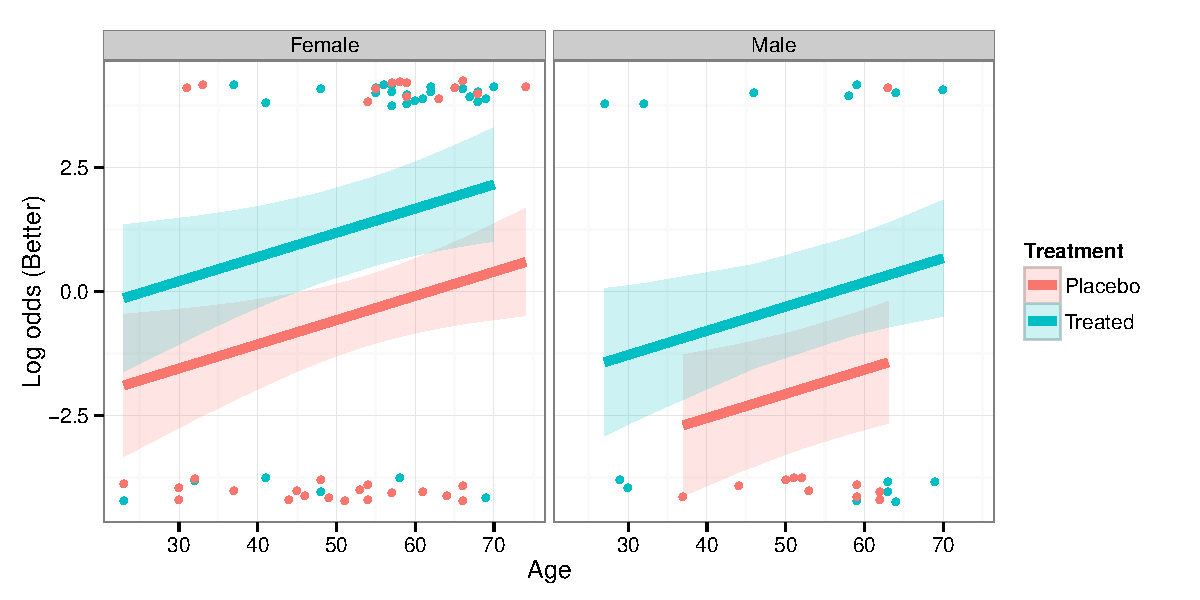
\includegraphics[width=.8\textwidth,clip]{ch07/fig/arth-full1-1} }

\caption[Full-model plot of Arthritis data, showing fitted logits by Treatment and Sex]{Full-model plot of Arthritis data, showing fitted logits by Treatment and Sex.\label{fig:arth-full1}}
\end{figure}


\end{knitrout}
This plot method has several nice features:
\begin{itemize*}
  \item Plotting on the logit scale shows the additive, linear effects of all predictors.
  \item It provides a visual representation of the information contained in the table of
  coefficients.  Note, however, that the choice to display \var{Treatment} within each
  panel makes it easier to judge the size of this effect, compared to the effect of
  \var{Sex} which must be judged across the panels.
  \item It shows the data as points, and the fitted lines and confidence bands are restricted
  to the range of the data in each.  You can easily see the reason for the unusual
  pattern in the conditional plot for Males shown in \figref{fig:arth-cond2}.
  \item It generalizes directly to any fitted model, because the same plotting code can
  be used once the model predicted values have been calculated.
  \item Additional predictors, either factors or quantitative variables can easily be
  accommodated by including them in the \func{facet\_wrap} call.  For example, if the
  patients were also categorized by education and this had been included in the model,
  \verb|facet_wrap(~ Sex + Education)| would produce separate panels for the combinations
  of these two variables.
\end{itemize*}

While plots on the logit scale have a simpler form, many people find it easier to think
about such relationships in terms of probabilities, as we have done in earlier plots
in this chapter.  You can do the same for full-model plots with a simple extension
of this method.  All you need to do is to transform the \code{fit} and
end points of the confidence band back to the scale of probabilities.
The  function \func{plogis} does this for the logistic
distribution.

\begin{knitrout}
\definecolor{shadecolor}{rgb}{1, 0.961, 0.933}\color{fgcolor}\begin{kframe}
\begin{alltt}
\hlstd{arth.fit2} \hlkwb{<-} \hlkwd{within}\hlstd{(arth.fit2, \{}
             \hlstd{prob}  \hlkwb{<-} \hlkwd{plogis}\hlstd{(fit)}
             \hlstd{lower} \hlkwb{<-} \hlkwd{plogis}\hlstd{(fit} \hlopt{-} \hlnum{1.96} \hlopt{*} \hlstd{se.fit)}
             \hlstd{upper} \hlkwb{<-} \hlkwd{plogis}\hlstd{(fit} \hlopt{+} \hlnum{1.96} \hlopt{*} \hlstd{se.fit)}
             \hlstd{\})}
\end{alltt}
\end{kframe}
\end{knitrout}
The plot step is then similar to what we used above (but with \code{prob}, \code{lower} and \code{upper}), producing \figref{fig:arth-full2}.
\begin{knitrout}
\definecolor{shadecolor}{rgb}{1, 0.961, 0.933}\color{fgcolor}\begin{kframe}
\begin{alltt}
\hlkwd{ggplot}\hlstd{( arth.fit2,} \hlkwd{aes}\hlstd{(}\hlkwc{x}\hlstd{=Age,} \hlkwc{y}\hlstd{=prob,} \hlkwc{color}\hlstd{=Treatment))} \hlopt{+}
  \hlkwd{geom_line}\hlstd{(}\hlkwc{size} \hlstd{=} \hlnum{2}\hlstd{)} \hlopt{+} \hlkwd{theme_bw}\hlstd{()} \hlopt{+}
  \hlkwd{geom_ribbon}\hlstd{(}\hlkwd{aes}\hlstd{(}\hlkwc{ymin} \hlstd{= lower,}
                  \hlkwc{ymax} \hlstd{= upper,}
                  \hlkwc{fill} \hlstd{= Treatment),} \hlkwc{alpha} \hlstd{=} \hlnum{0.2}\hlstd{,}
              \hlkwc{color} \hlstd{=} \hlstr{"transparent"}\hlstd{)} \hlopt{+}
  \hlkwd{labs}\hlstd{(}\hlkwc{x} \hlstd{=} \hlstr{"Age"}\hlstd{,} \hlkwc{y} \hlstd{=} \hlstr{"Probability (Better)"}\hlstd{)} \hlopt{+}
  \hlkwd{geom_point}\hlstd{(}\hlkwd{aes}\hlstd{(}\hlkwc{y}\hlstd{=Better),}
             \hlkwc{position}\hlstd{=}\hlkwd{position_jitter}\hlstd{(}\hlkwc{height}\hlstd{=}\hlnum{0.02}\hlstd{,} \hlkwc{width}\hlstd{=}\hlnum{0}\hlstd{))} \hlopt{+}
  \hlkwd{facet_wrap}\hlstd{(}\hlopt{~} \hlstd{Sex)}
\end{alltt}
\end{kframe}\begin{figure}[!htbp]


\centerline{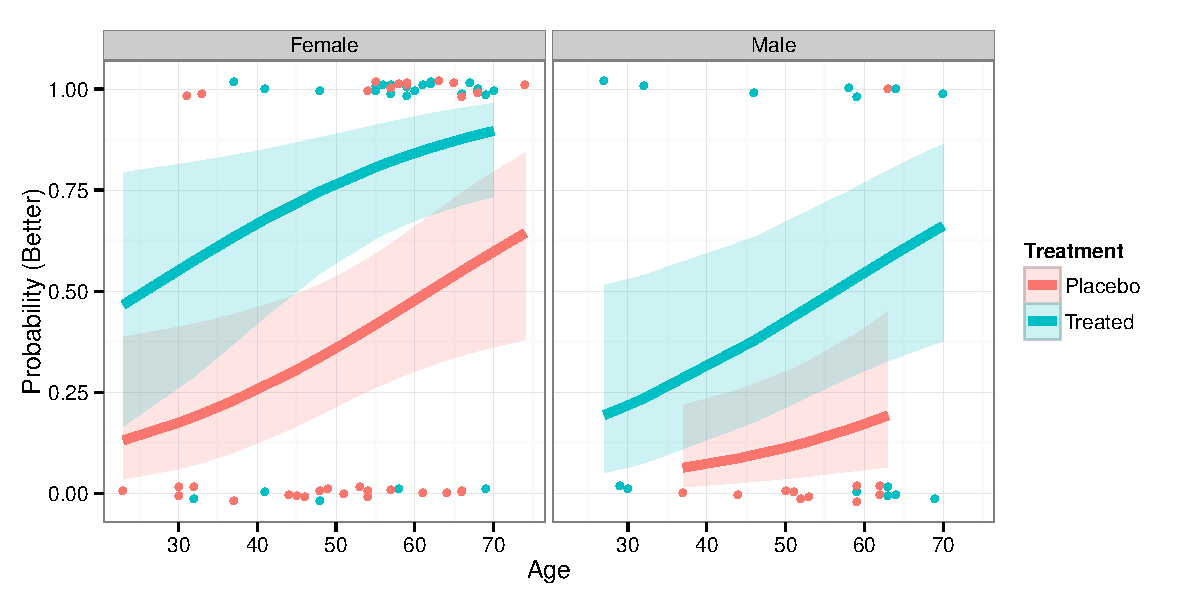
\includegraphics[width=.8\textwidth,clip]{ch07/fig/arth-full2-1} }

\caption[Full-model plot of Arthritis data, showing fitted probabilities by Treatment and Sex]{Full-model plot of Arthritis data, showing fitted probabilities by Treatment and Sex.\label{fig:arth-full2}}
\end{figure}


\end{knitrout}

\end{Example}

\subsection{Effect plots}\label{sec:logist-effplots}
For more than two variables, full-model plots of the fitted response surface can
be cumbersome, particularly when the model contains interactions or when the main
substantive interest is focused on a given main effect or interaction, controlling
for all other explanatory variables.
The method of \term{effect displays} (tables and graphs), developed by
John Fox \citeyearpar{Fox:87,Fox:03:effects} and implemented in the \Rpackage{effects},
is a useful solution to these problems.

The idea of effect plots is quite simple but very general:% 
\footnote{
Less general expression of these ideas include the use of \term{adjusted means}
in analysis of covariance, and \term{least squares means} 
or \term{population marginal means} \citep{Searle-etal:80}
in analysis of variance; for example, see the \Rpackage{lsmeans} for classical linear models.
}
consider a particular
subset of predictors (\emph{focal predictors}) we wish to visualize in a given
linear model or generalized linear model.  The essence is to calculate fitted
values (and standard errors) for the model terms involving these variables
and all low-order relatives (e.g., main effects that are marginal to an interaction),
as these variables are allowed to vary over their range.  All other variables
are ``controlled'' by being fixed at typical values. For example a quantitative
covariate could be fixed at its mean or median; a factor could be fixed at
equal proportions of its levels or its proportions in the data.
The result, when plotted, shows all effects of the focal predictors and their
low-order relatives, but with all other variables not included controlled or
adjusted for.

More formally, assume we have fit a model with a linear predictor
$\eta_i =  \alpha + \vec{x}_{i}\trans \,  \vec{\beta} $ 
(on the logit scale, for logistic regression).
Letting $\beta_0 = \alpha$ and $\vec{x}_0 = \vec{1}$, we can rewrite this
in matrix form as $\vec{\eta} = \mat{X} \vec{\beta}$ where $\mat{X}$ is
the model matrix constructed by the modeling function, such as \func{glm}.
Fitting the model gives the estimated coefficients $\vec{b}$ and
its estimated covariance matrix $\widehat{\mat{\V} (\vec{b})}$.

The \func{Effect} function constructs an analogous \emph{score model matrix},
$\mat{X}^*$, where the focal variables have been varied over their range,
and all other variables represented as constant, typical values.
Using this as input (the \code{newdata} argument)
to the \func{predict} function then gives the 
fitted values $\vec{\eta}^* = \mat{X}^* \vec{b}$.
Standard errors used for confidence intervals are calculated by
\func{predict} (when \code{se.fit=TRUE}) as the square roots of
$\diag (\mat{X}^* \widehat{\mat{\V} (\vec{b})} \mat{X}^{*\mathsf{T}} )$.
Note that these ideas work not only for \func{glm} models, but potentially for
any modeling function that has a \func{predict} and \func{vcov} method.%
\footnote{
For example, the \Rpackage{effects} presently provides methods for models fit by
\func{lm} (including multivariate linear response models), \func{glm},
\func{gls}, multinomial (\func{multinom} in the \Rpackage{nnet})
and proportional odds models (\func{polr} in \pkg{MASS}),
polytomous latent class models (\Rpackage{poLCA}), as well as
a variety of multi-level and mixed-effects linear models fit with
\func{lmer} from the \Rpackage{lme4}, or with \func{lme} from the \Rpackage{nlme}.
}

These results are calculated on the scale of the linear predictor $\vec{\eta}$
(logits, for logistic regression) when the \code{type} argument to
\func{predict} is \code{type="link"} or on the response scale
(probabilities, here) when \code{type="response"}.  The latter makes use
of the inverse transformation, \eqref{eq:logistm1}.  

There are two main calculation functions in the \Rpackage{effects}:

\begin{itemize}
\item \func{Effect} takes a character vector of the names of a subset of focal predictors
and constructs the score matrix $\mat{X}^*$ by varying these over their ranges,
while holding all other predictors constant at ``typical'' values.
There are many options that control these calculations. For example,
\code{xlevels} can be used to specify the values of the focal predictors; 
\code{typical} or \code{given.values} respectively can be used to specify either a
function (\code{mean}, \code{median}) or a list of specific typical values
used for the variables that are controlled.
The result is an object of class \class{eff}, for which there are \func{print},
\func{summary} and (most importantly) \func{plot} methods.  See \help{Effect}
for a complete description.

\item \func{allEffects} takes a model object, and calculates the effects for each
high-order term in the model (including their low-order) relatives.  Similar
optional arguments control the details of the computation. 
The result is an object of class \class{efflist}.
\end{itemize}

In addition, the plotting methods for \class{eff} and \class{efflist} objects offer
numerous options to control the plot details, only a few of which are used in the
examples below. For logistic regression models, they also solve the problem of
the trade-off between plots on the logit scale, that have a simple representation
in terms of additive effects, and plots on the probability scale that are
usually simpler to understand.  By default, the fitted model effects are 
plotted on the logit scale, but the response $y$ axis is labeled with 
the corresponding probability values.

\begin{Example}[arthrit-eff]{Arthritis treatment}
Here we illustrate the use of the \Rpackage{effects} with the simple main effects
model which was fit in \exref{ex:arthrit-mult}.  \func{allEffects} is used to 
calculate the predicted probabilities of the \var{Better} response for
\var{Age} and the two factors, \var{Sex} and \var{Treatment}. 
\begin{knitrout}
\definecolor{shadecolor}{rgb}{1, 0.961, 0.933}\color{fgcolor}\begin{kframe}
\begin{alltt}
\hlkwd{library}\hlstd{(effects)}
\hlstd{arth.eff2} \hlkwb{<-} \hlkwd{allEffects}\hlstd{(arth.logistic2)}
\hlkwd{names}\hlstd{(arth.eff2)}
\end{alltt}
\begin{verbatim}
## [1] "I(Age-50)" "Sex"       "Treatment"
\end{verbatim}
\end{kframe}
\end{knitrout}
The result, \code{arth.eff2} is a list containing the fitted values (response probabilities, by default)
for each of the the model terms. No \code{xlevels} argument was specified, so by default
the function calculated the effects for \var{Age} at a reasonable selection of equally-spaced
values:
\begin{knitrout}
\definecolor{shadecolor}{rgb}{1, 0.961, 0.933}\color{fgcolor}\begin{kframe}
\begin{alltt}
\hlstd{arth.eff2[[}\hlnum{1}\hlstd{]]}
\end{alltt}
\begin{verbatim}
## 
##  Age effect
## Age
##      30      40      50      60      70 
## 0.24289 0.34311 0.45959 0.58066 0.69274
\end{verbatim}
\end{kframe}
\end{knitrout}
The default plot method for the \class{efflist} object produces one plot for each high-order
term, which are just the main effect in this model.  The call below produces
\figref{fig:arth-effplot1}.
\begin{knitrout}
\definecolor{shadecolor}{rgb}{1, 0.961, 0.933}\color{fgcolor}\begin{kframe}
\begin{alltt}
\hlkwd{plot}\hlstd{(arth.eff2,} \hlkwc{rows}\hlstd{=}\hlnum{1}\hlstd{,} \hlkwc{cols}\hlstd{=}\hlnum{3}\hlstd{)}
\end{alltt}
\end{kframe}\begin{figure}[!htbp]


\centerline{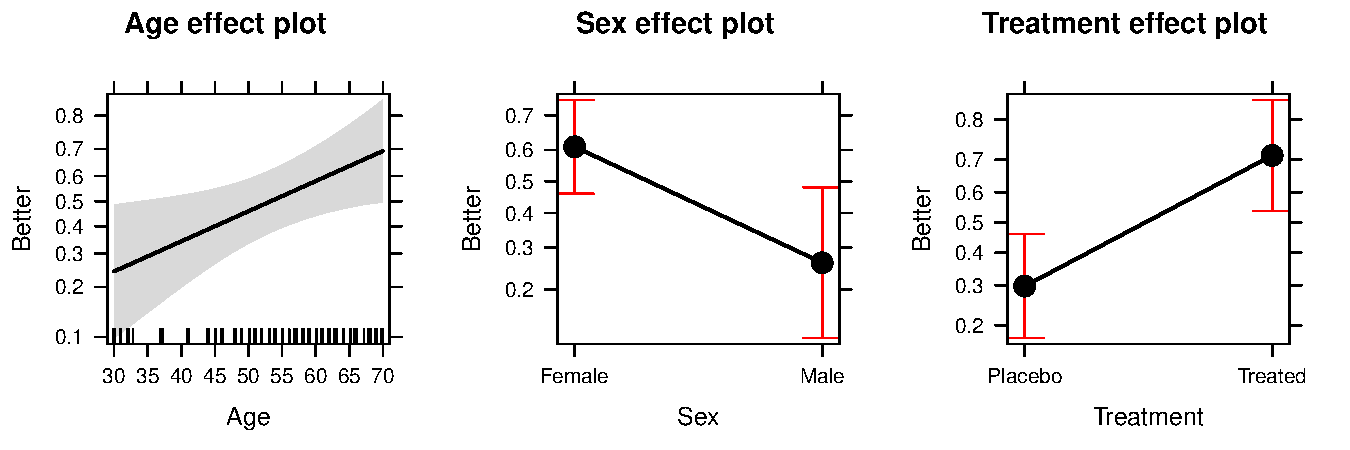
\includegraphics[width=\textwidth]{ch07/fig/arth-effplot1-1} }

\caption[Plot of all effects in the main effects model for the Arthritis data]{Plot of all effects in the main effects model for the Arthritis data\label{fig:arth-effplot1}}
\end{figure}


\end{knitrout}

You can also produce full-model plots quite easily by using all predictors in the model
in a call to \func{Effect}.
\begin{knitrout}
\definecolor{shadecolor}{rgb}{1, 0.961, 0.933}\color{fgcolor}\begin{kframe}
\begin{alltt}
\hlstd{arth.full} \hlkwb{<-} \hlkwd{Effect}\hlstd{(}\hlkwd{c}\hlstd{(}\hlstr{"Age"}\hlstd{,} \hlstr{"Treatment"}\hlstd{,} \hlstr{"Sex"}\hlstd{), arth.logistic2)}
\end{alltt}
\end{kframe}
\end{knitrout}
Then plotting the result, with some options, gives the plot shown in \figref{fig:arth-effplot2}.
\begin{knitrout}
\definecolor{shadecolor}{rgb}{1, 0.961, 0.933}\color{fgcolor}\begin{kframe}
\begin{alltt}
\hlkwd{plot}\hlstd{(arth.full,} \hlkwc{multiline}\hlstd{=}\hlnum{TRUE}\hlstd{,} \hlkwc{ci.style}\hlstd{=}\hlstr{"bands"}\hlstd{,}
     \hlkwc{colors} \hlstd{=} \hlkwd{c}\hlstd{(}\hlstr{"red"}\hlstd{,} \hlstr{"blue"}\hlstd{),} \hlkwc{lwd}\hlstd{=}\hlnum{3}\hlstd{,}
     \hlkwc{key.args}\hlstd{=}\hlkwd{list}\hlstd{(}\hlkwc{x}\hlstd{=}\hlnum{.52}\hlstd{,} \hlkwc{y}\hlstd{=}\hlnum{.92}\hlstd{),} \hlkwc{grid}\hlstd{=}\hlnum{TRUE}\hlstd{)}
\end{alltt}
\end{kframe}\begin{figure}[!htbp]


\centerline{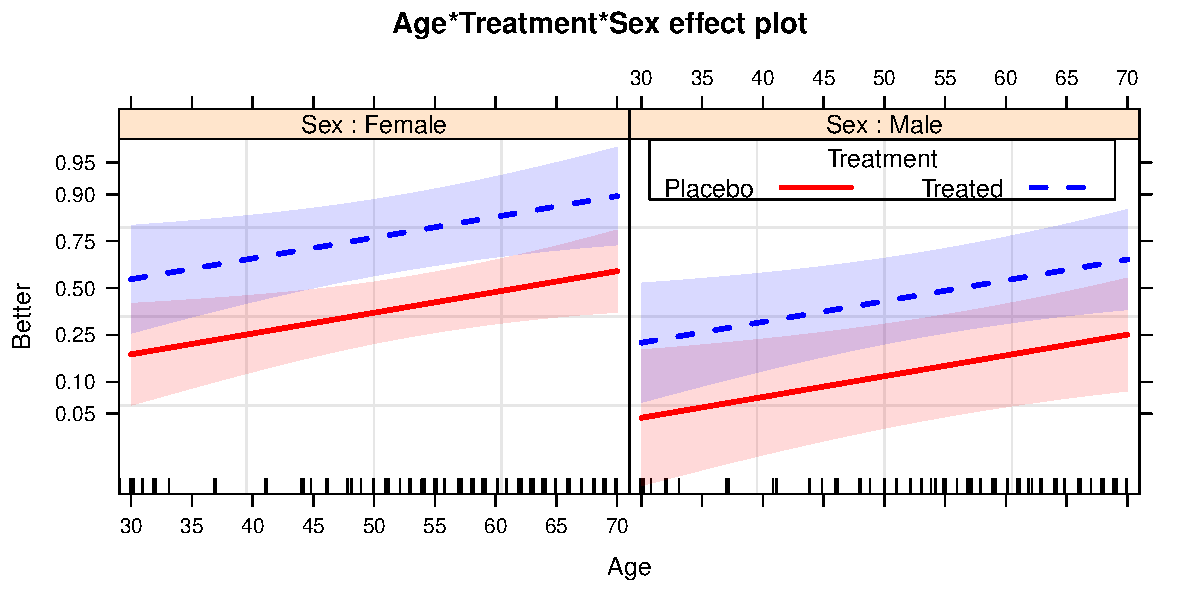
\includegraphics[width=.8\textwidth]{ch07/fig/arth-effplot2-1} }

\caption[Full-model plot of the effects of all predictors in the main effects model for the Arthritis data, plotted on the logit scale]{Full-model plot of the effects of all predictors in the main effects model for the Arthritis data, plotted on the logit scale.\label{fig:arth-effplot2}}
\end{figure}


\end{knitrout}
Alternatively, we can plot these results directly on the scale of probabilities, as
shown in \figref{fig:arth-effplot3}.
\begin{knitrout}
\definecolor{shadecolor}{rgb}{1, 0.961, 0.933}\color{fgcolor}\begin{kframe}
\begin{alltt}
\hlkwd{plot}\hlstd{(arth.full,} \hlkwc{multiline}\hlstd{=}\hlnum{TRUE}\hlstd{,} \hlkwc{ci.style}\hlstd{=}\hlstr{"bands"}\hlstd{,} \hlkwc{rescale.axis}\hlstd{=}\hlnum{FALSE}\hlstd{,}
     \hlkwc{colors} \hlstd{=} \hlkwd{c}\hlstd{(}\hlstr{"red"}\hlstd{,} \hlstr{"blue"}\hlstd{),} \hlkwc{lwd}\hlstd{=}\hlnum{3}\hlstd{,}
     \hlkwc{key.args}\hlstd{=}\hlkwd{list}\hlstd{(}\hlkwc{x}\hlstd{=}\hlnum{.52}\hlstd{,} \hlkwc{y}\hlstd{=}\hlnum{.92}\hlstd{),} \hlkwc{grid}\hlstd{=}\hlnum{TRUE}\hlstd{)}
\end{alltt}
\end{kframe}\begin{figure}[!htbp]


\centerline{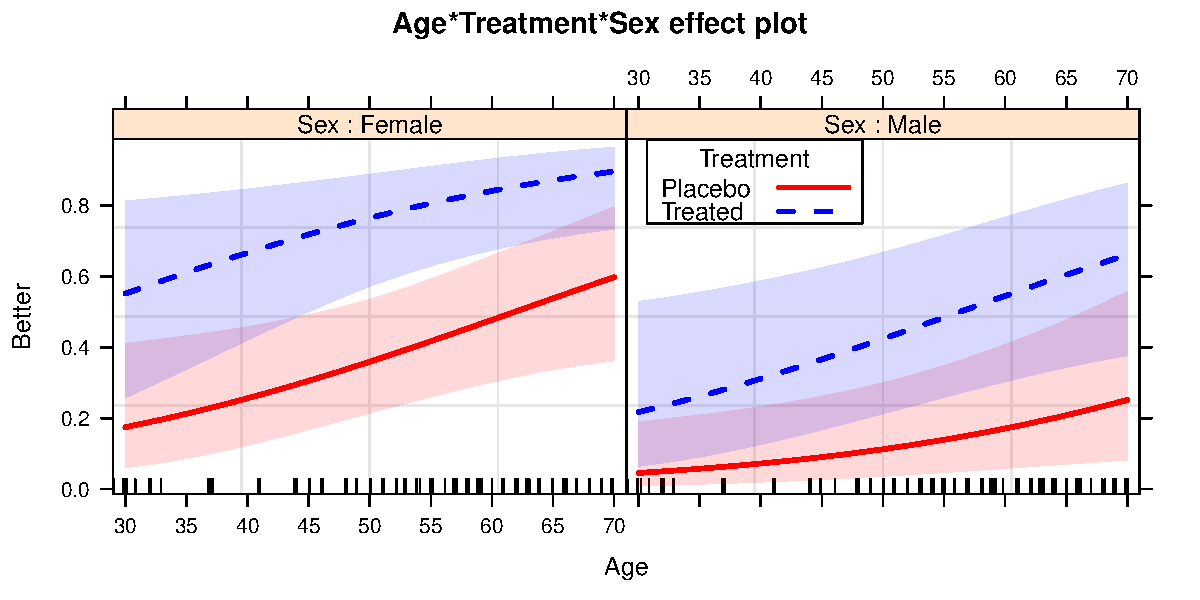
\includegraphics[width=.8\textwidth]{ch07/fig/arth-effplot3-1} }

\caption[Full-model plot of the effects of all predictors in the main effects model for the Arthritis data, plotted on the probability scale]{Full-model plot of the effects of all predictors in the main effects model for the Arthritis data, plotted on the probability scale.\label{fig:arth-effplot3}}
\end{figure}


\end{knitrout}

\end{Example}

\section{Case studies}

The examples below take up some issues of data analysis, model building and visualization
in the context of multiple logistic regression models.  We focus on the combination of
exploratory plots to see the data, modeling steps and graphs to interpret a given model.


\begin{Example}[donner1]{Donner Party}

In \chref{ch:intro}, \exref{ex:donner0}, we described the background behind the
sad story of the Donner Party, perhaps
the most famous tragedy in the history of the westward settlement in the United States. In brief, the party was stranded on the eastern side of the
Sierra Nevada mountains by heavy snow in late October, 1846, and by
the time the last survivor was rescued in April, 1847, nearly half
of the members had died from famine and exposure to extreme cold.
\figref{fig:donner0} showed that survival decreased strongly with age.

Here we consider a more detailed analysis of these data, which are contained in the
data set \data{Donner} in \pkg{vcdExtra}.  This data set lists 90 people in
the Donner Party by name, together with age, sex, survived (0/1) and the date of
death for those who died.%
\footnote{
Most historical sources count the number in the Donner Party at 87 or 89.
An exact accounting of the members of the Donner Party is difficult, because:
\begin{seriate}
 \item several people joined the party in mid-route, at Fort Bridger and in the
Wasatch Mountains; 
 \item several rode ahead to search for supplies and one (Charles Stanton)
 brought two more with him (Luis and Salvador);
 \item five people died before reaching the Sierra Nevada mountains.
\end{seriate}
It incorporates updated information from Kristin Johnson's
listing, \url{http://user.xmission.com/~octa/DonnerParty/Roster.htm}.
}

\begin{knitrout}
\definecolor{shadecolor}{rgb}{1, 0.961, 0.933}\color{fgcolor}\begin{kframe}
\begin{alltt}
\hlkwd{data}\hlstd{(}\hlstr{"Donner"}\hlstd{,} \hlkwc{package}\hlstd{=}\hlstr{"vcdExtra"}\hlstd{)}   \hlcom{# load the data}
\hlkwd{library}\hlstd{(car)}                         \hlcom{# for some() and Anova()}
\hlkwd{some}\hlstd{(Donner,} \hlnum{8}\hlstd{)}
\end{alltt}
\begin{verbatim}
##                       family age    sex survived      death
## Breen, Peter           Breen   3   Male        1       <NA>
## Donner, Jacob         Donner  65   Male        0 1846-12-21
## Foster, Jeremiah   MurFosPik   1   Male        0 1847-03-13
## Graves, Nancy         Graves   9 Female        1       <NA>
## McCutchen, Harriet McCutchen   1 Female        0 1847-02-02
## Reed, James             Reed  46   Male        1       <NA>
## Reinhardt, Joseph      Other  30   Male        0 1846-12-21
## Wolfinger, Doris    FosdWolf  20 Female        1       <NA>
\end{verbatim}
\end{kframe}
\end{knitrout}

The main purpose of this example is to try to understand, through graphs and models, how survival
was related to age and sex. However, first, we do some data preparation and exploration.
The response variable, \var{survived} is a 0/1 integer, and it is more convenient for some purposes to
make it a factor.
\begin{knitrout}
\definecolor{shadecolor}{rgb}{1, 0.961, 0.933}\color{fgcolor}\begin{kframe}
\begin{alltt}
\hlstd{Donner}\hlopt{$}\hlstd{survived} \hlkwb{<-} \hlkwd{factor}\hlstd{(Donner}\hlopt{$}\hlstd{survived,} \hlkwc{labels}\hlstd{=}\hlkwd{c}\hlstd{(}\hlstr{"no"}\hlstd{,} \hlstr{"yes"}\hlstd{))}
\end{alltt}
\end{kframe}
\end{knitrout}

Some historical accounts \citep{Grayson:1990} link survival in the Donner Party to
kinship or family groups, so we take a quick look at this factor here.
The variable \var{family}
reflects a recoding of the last names of individuals to reduce the number of factor levels. 
The main families in the Donner party were: Donner, Graves, Breen and Reed. 
The families of Murphy, Foster and Pike are grouped as \code{"MurFosPik"}, 
those of Fosdick and Wolfinger are coded as \code{"FosdWolf"}, and all others as 
\code{"Other"}. 

\begin{knitrout}
\definecolor{shadecolor}{rgb}{1, 0.961, 0.933}\color{fgcolor}\begin{kframe}
\begin{alltt}
\hlkwd{xtabs}\hlstd{(}\hlopt{~}\hlstd{family,} \hlkwc{data}\hlstd{=Donner)}
\end{alltt}
\begin{verbatim}
## family
##     Breen    Donner      Eddy  FosdWolf    Graves  Keseberg 
##         9        14         4         4        10         4 
## McCutchen MurFosPik     Other      Reed 
##         3        12        23         7
\end{verbatim}
\end{kframe}
\end{knitrout}
For the present purposes, we reduce these 10 family groups further, collapsing some of
the small families into \code{"Other"}, 
and reordering the levels.  Assigning new values to the \func{levels} of a factor
is a convenient trick for recoding factor variables.
\begin{knitrout}
\definecolor{shadecolor}{rgb}{1, 0.961, 0.933}\color{fgcolor}\begin{kframe}
\begin{alltt}
\hlcom{# collapse small families into "Other"}
\hlstd{fam} \hlkwb{<-} \hlstd{Donner}\hlopt{$}\hlstd{family}
\hlkwd{levels}\hlstd{(fam)[}\hlkwd{c}\hlstd{(}\hlnum{3}\hlstd{,}\hlnum{4}\hlstd{,}\hlnum{6}\hlstd{,}\hlnum{7}\hlstd{,}\hlnum{9}\hlstd{)]} \hlkwb{<-} \hlstr{"Other"}

\hlcom{# reorder, putting Other last}
\hlstd{fam} \hlkwb{=} \hlkwd{factor}\hlstd{(fam,}\hlkwd{levels}\hlstd{(fam)[}\hlkwd{c}\hlstd{(}\hlnum{1}\hlstd{,} \hlnum{2}\hlstd{,} \hlnum{4}\hlopt{:}\hlnum{6}\hlstd{,} \hlnum{3}\hlstd{)])}
\hlstd{Donner}\hlopt{$}\hlstd{family} \hlkwb{<-} \hlstd{fam}
\hlkwd{xtabs}\hlstd{(}\hlopt{~}\hlstd{family,} \hlkwc{data}\hlstd{=Donner)}
\end{alltt}
\begin{verbatim}
## family
##     Breen    Donner    Graves MurFosPik      Reed     Other 
##         9        14        10        12         7        38
\end{verbatim}
\end{kframe}
\end{knitrout}
\func{xtabs} then shows the counts of survival by these family groups:
\begin{knitrout}
\definecolor{shadecolor}{rgb}{1, 0.961, 0.933}\color{fgcolor}\begin{kframe}
\begin{alltt}
\hlkwd{xtabs}\hlstd{(}\hlopt{~}\hlstd{survived}\hlopt{+}\hlstd{family,} \hlkwc{data}\hlstd{=Donner)}
\end{alltt}
\begin{verbatim}
##         family
## survived Breen Donner Graves MurFosPik Reed Other
##      no      0      7      3         6    1    25
##      yes     9      7      7         6    6    13
\end{verbatim}
\end{kframe}
\end{knitrout}
Plotting this distribution of  survival by family with a formula gives a \term{spineplot}, a 
special case of the mosaic plot, or a generalization of a stacked bar plot,
shown in \figref{fig:donner1-spineplot}.
The widths of the bars are proportional to family size, and the shading highlights in light blue
the proportion who survived in each family.
\begin{knitrout}
\definecolor{shadecolor}{rgb}{1, 0.961, 0.933}\color{fgcolor}\begin{kframe}
\begin{alltt}
\hlkwd{plot}\hlstd{(survived} \hlopt{~} \hlstd{family,} \hlkwc{data}\hlstd{=Donner,} \hlkwc{col}\hlstd{=}\hlkwd{c}\hlstd{(}\hlstr{"pink"}\hlstd{,} \hlstr{"lightblue"}\hlstd{))}
\end{alltt}
\end{kframe}\begin{figure}[!htbp]


\centerline{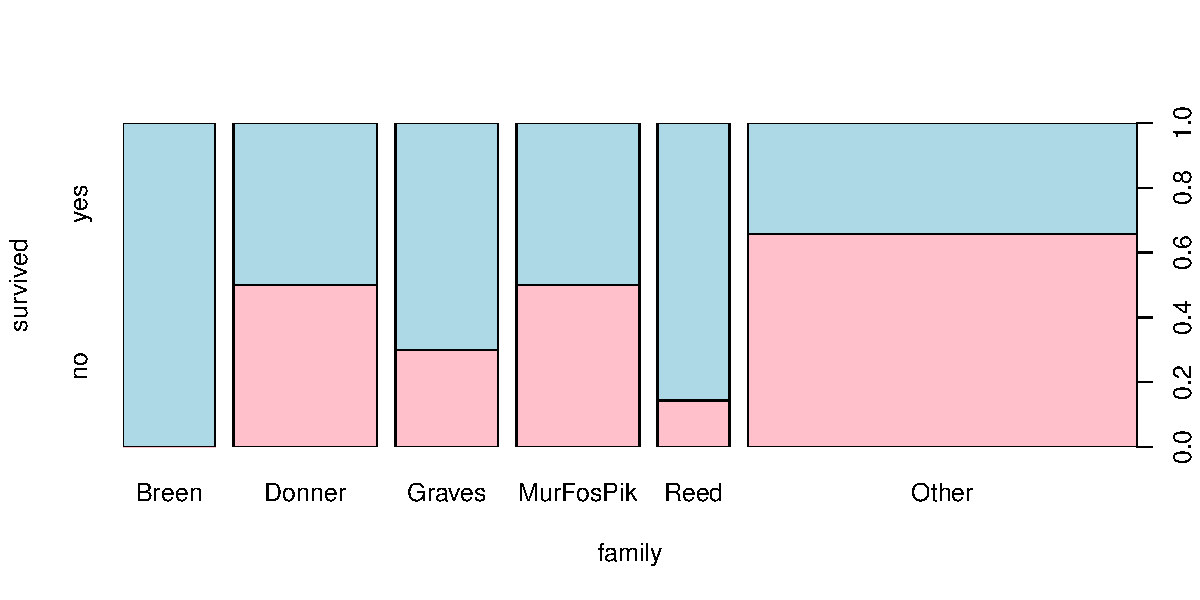
\includegraphics[width=.8\textwidth]{ch07/fig/donner1-spineplot-1} }

\caption[Spineplot of survival in the Donner Party by family]{Spineplot of survival in the Donner Party by family.\label{fig:donner1-spineplot}}
\end{figure}


\end{knitrout}

% Another exploratory, smoothing plot for discrete response data
% is the \term{conditional density plot},
% showing how the conditional distribution of a categorical variable $Y$ changes over a numerical variable $x$. \func{cdplot} computes and plots $\Pr(Y \given x) against $x$.

% the conditional densities of x given the levels of y weighted by the marginal distribution of y. The densities are derived cumulatively over the levels of y.
% 
% This visualization technique is similar to spinograms (see spineplot) and plots P(y | x) against x. The conditional probabilities are not derived by discretization (as in the spinogram), but using a smoothing approach via density.
% 
% Note, that the estimates of the conditional densities are more reliable for high-density regions of x. Conversely, the are less reliable in regions with only few x observations.

A generalized pairs plot (\secref{sec:condmat}), shown in \figref{fig:donner1-gpairs} gives a visual
overview of the data.  The diagonal panels here show the marginal distributions of the variables
as bar plots, and highlight the skewed distribution of age and the greater number of males
than females in the party.  The boxplots and barcode plots for survived and age show
that those who survived were generally younger than those who perished.
\begin{knitrout}
\definecolor{shadecolor}{rgb}{1, 0.961, 0.933}\color{fgcolor}\begin{kframe}
\begin{alltt}
\hlkwd{library}\hlstd{(gpairs)}
\hlkwd{library}\hlstd{(vcd)}
\hlkwd{gpairs}\hlstd{(Donner[,}\hlkwd{c}\hlstd{(}\hlnum{4}\hlstd{,}\hlnum{2}\hlstd{,}\hlnum{3}\hlstd{,}\hlnum{1}\hlstd{)],}
  \hlkwc{diag.pars}\hlstd{=}\hlkwd{list}\hlstd{(}\hlkwc{fontsize}\hlstd{=}\hlnum{20}\hlstd{,} \hlkwc{hist.color}\hlstd{=}\hlstr{"gray"}\hlstd{),}
        \hlkwc{mosaic.pars}\hlstd{=}\hlkwd{list}\hlstd{(}\hlkwc{gp}\hlstd{=shading_Friendly),} \hlkwc{outer.rot}\hlstd{=}\hlkwd{c}\hlstd{(}\hlnum{45}\hlstd{,}\hlnum{45}\hlstd{)}
        \hlstd{)}
\end{alltt}
\end{kframe}\begin{figure}[!htbp]


\centerline{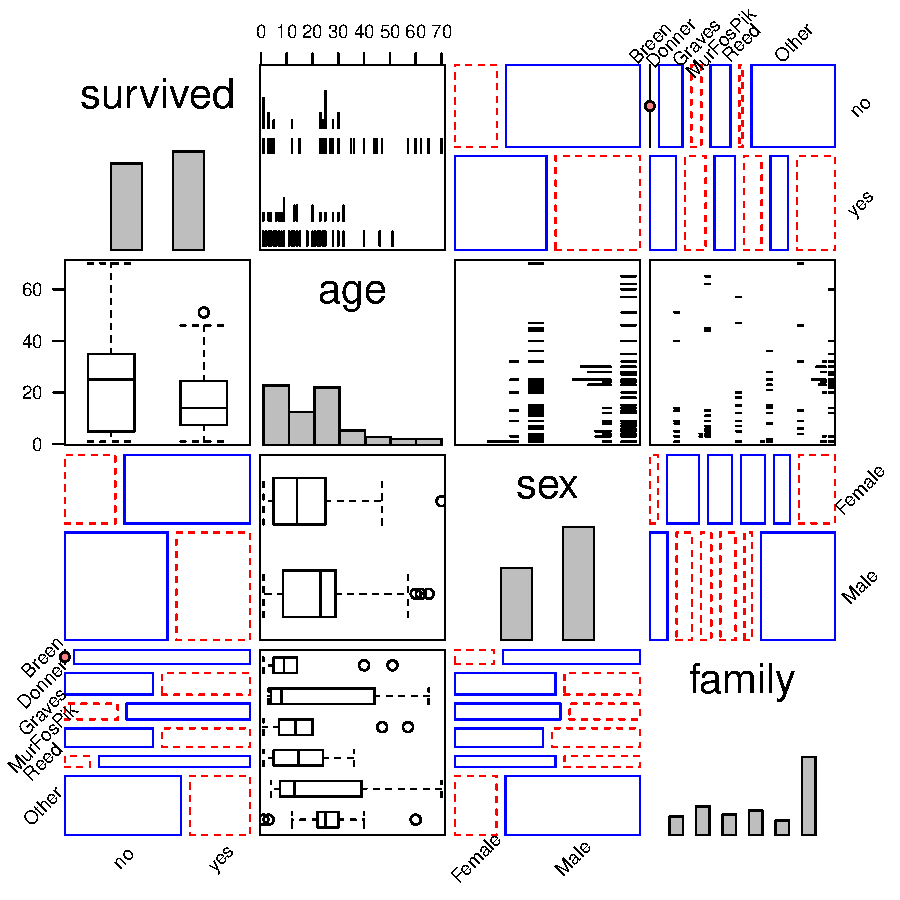
\includegraphics[width=.7\textwidth]{ch07/fig/donner1-gpairs-1} }

\caption[Generalized pairs plot for the Donner data]{Generalized pairs plot for the Donner data\label{fig:donner1-gpairs}}
\end{figure}


\end{knitrout}


From an exploratory perspective,
we now proceed to examine the relationship of survival to age and sex, beginning with the
kind of conditional plots we illustrated earlier (in \exref{ex:arth-cond}).
\figref{fig:donner1-cond1} shows a plot of \var{survived}, converted back to
a 0/1 variable as required by \func{ggplot}, together with the binary responses
as points and the fitted logistic regressions separately for males and females.

\begin{knitrout}
\definecolor{shadecolor}{rgb}{1, 0.961, 0.933}\color{fgcolor}\begin{kframe}
\begin{alltt}
\hlkwd{ggplot}\hlstd{(Donner,} \hlkwd{aes}\hlstd{(age,} \hlkwd{as.numeric}\hlstd{(survived}\hlopt{==}\hlstr{"yes"}\hlstd{),} \hlkwc{color} \hlstd{= sex))} \hlopt{+}
  \hlkwd{theme_bw}\hlstd{()} \hlopt{+} \hlkwd{ylab}\hlstd{(}\hlstr{"Survived"}\hlstd{)} \hlopt{+}
  \hlkwd{geom_point}\hlstd{(}\hlkwc{position} \hlstd{=} \hlkwd{position_jitter}\hlstd{(}\hlkwc{height} \hlstd{=} \hlnum{0.02}\hlstd{,} \hlkwc{width} \hlstd{=} \hlnum{0}\hlstd{))} \hlopt{+}
  \hlkwd{stat_smooth}\hlstd{(}\hlkwc{method} \hlstd{=} \hlstr{"glm"}\hlstd{,} \hlkwc{family} \hlstd{= binomial,} \hlkwc{formula} \hlstd{= y} \hlopt{~} \hlstd{x,}
              \hlkwc{alpha} \hlstd{=} \hlnum{0.2}\hlstd{,} \hlkwc{size}\hlstd{=}\hlnum{2}\hlstd{,} \hlkwd{aes}\hlstd{(}\hlkwc{fill} \hlstd{= sex))}
\end{alltt}
\end{kframe}\begin{figure}[!htbp]


\centerline{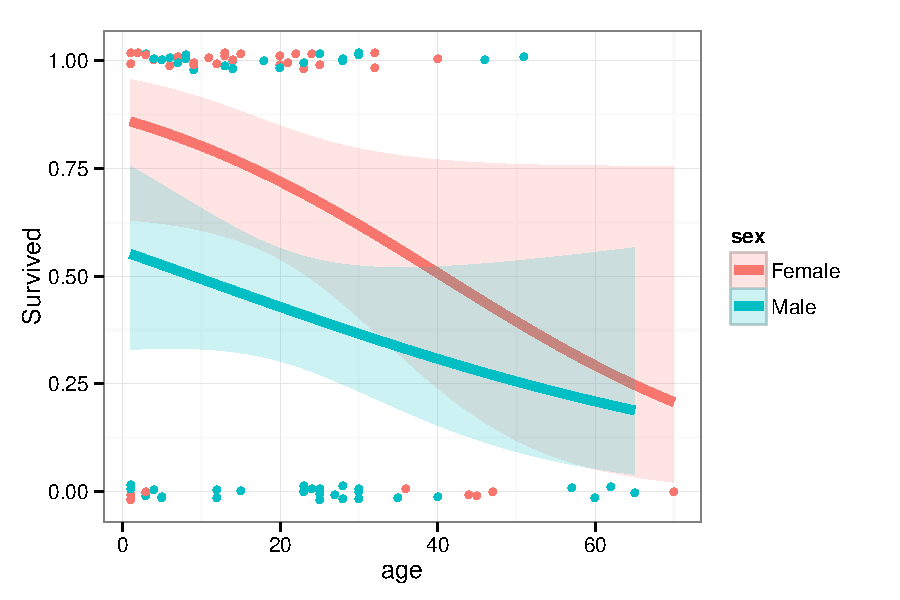
\includegraphics[width=.7\textwidth]{ch07/fig/donner1-cond1-1} }

\caption[Conditional plot of the Donner data, showing the relationship of survival to age and sex]{Conditional plot of the Donner data, showing the relationship of survival to age and sex. The smoothed curves and confidence bands show the result of fitting separate linear logistic regressions on age for males and females.\label{fig:donner1-cond1}}
\end{figure}


\end{knitrout}
It is easy to see that survival among women was greater that that for men,
perhaps narrowing the gap among the older people, but the data gets thin
towards the upper range of age.

The curves plotted in \figref{fig:donner1-cond1} assume a linear relationship between
the log odds of survival and age (expressed as \verb|formula = y ~ x| in the call to
\func{stat\_smooth}).  One simple way to check whether the relationship between
survival and age is non-linear is to re-do this plot, but now allow a quadratic
relationship with age, using \verb|formula = y ~ poly(x,2)|. The result is shown
in the left panel of \figref{fig:donner1-cond3}.

% <<donner1-cond2, h=4, w=6, out.width='.7\\textwidth', cap='Conditional plot of the Donner data, showing the relationship of survival to age and sex. The smoothed curves and confidence bands now show the result of fitting separate quadratic logistic regressions on age for males and females.'>>=
% ggplot(Donner, aes(age, as.numeric(survived=="yes"), color = sex)) + 
%   theme_bw() + ylab("Survived") +
%   geom_point(position = position_jitter(height = 0.02, width = 0)) +
%   stat_smooth(method = "glm", family = binomial, formula = y ~ poly(x,2),
%               alpha = 0.2, size=2, aes(fill = sex))
% 
% @
\begin{knitrout}
\definecolor{shadecolor}{rgb}{1, 0.961, 0.933}\color{fgcolor}\begin{kframe}
\begin{alltt}
\hlstd{gg} \hlkwb{<-} \hlkwd{ggplot}\hlstd{(Donner,} \hlkwd{aes}\hlstd{(age,} \hlkwd{as.numeric}\hlstd{(survived}\hlopt{==}\hlstr{"yes"}\hlstd{),} \hlkwc{color} \hlstd{= sex))} \hlopt{+}
  \hlkwd{theme_bw}\hlstd{()} \hlopt{+} \hlkwd{ylab}\hlstd{(}\hlstr{"Survived"}\hlstd{)} \hlopt{+}
  \hlkwd{geom_point}\hlstd{(}\hlkwc{position} \hlstd{=} \hlkwd{position_jitter}\hlstd{(}\hlkwc{height} \hlstd{=} \hlnum{0.02}\hlstd{,} \hlkwc{width} \hlstd{=} \hlnum{0}\hlstd{))}

\hlstd{gg} \hlopt{+} \hlkwd{stat_smooth}\hlstd{(}\hlkwc{method} \hlstd{=} \hlstr{"glm"}\hlstd{,} \hlkwc{family} \hlstd{= binomial,} \hlkwc{formula} \hlstd{= y} \hlopt{~} \hlkwd{poly}\hlstd{(x,}\hlnum{2}\hlstd{),}
                 \hlkwc{alpha} \hlstd{=} \hlnum{0.2}\hlstd{,} \hlkwc{size}\hlstd{=}\hlnum{2}\hlstd{,} \hlkwd{aes}\hlstd{(}\hlkwc{fill} \hlstd{= sex))}

\hlstd{gg} \hlopt{+} \hlkwd{stat_smooth}\hlstd{(}\hlkwc{method} \hlstd{=} \hlstr{"loess"}\hlstd{,} \hlkwc{span}\hlstd{=}\hlnum{0.9}\hlstd{,} \hlkwc{alpha} \hlstd{=} \hlnum{0.2}\hlstd{,} \hlkwc{size}\hlstd{=}\hlnum{2}\hlstd{,}
                 \hlkwd{aes}\hlstd{(}\hlkwc{fill} \hlstd{= sex))} \hlopt{+} \hlkwd{coord_cartesian}\hlstd{(}\hlkwc{ylim}\hlstd{=}\hlkwd{c}\hlstd{(}\hlopt{-}\hlnum{.05}\hlstd{,}\hlnum{1.05}\hlstd{))}
\end{alltt}
\end{kframe}\begin{figure}[!htbp]


\centerline{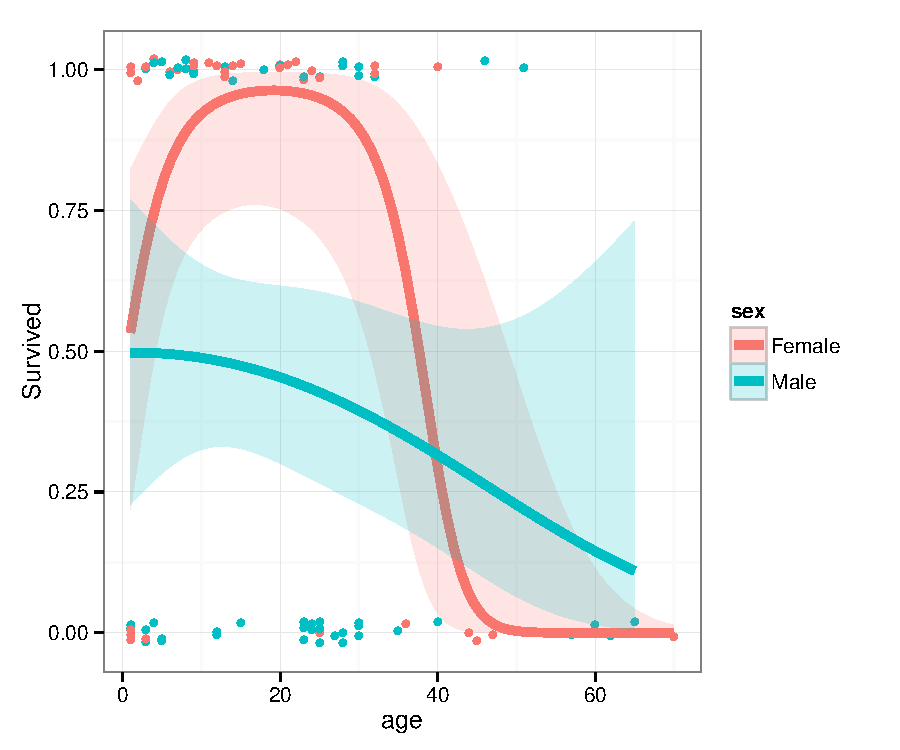
\includegraphics[width=.5\textwidth]{ch07/fig/donner1-cond3-1} 
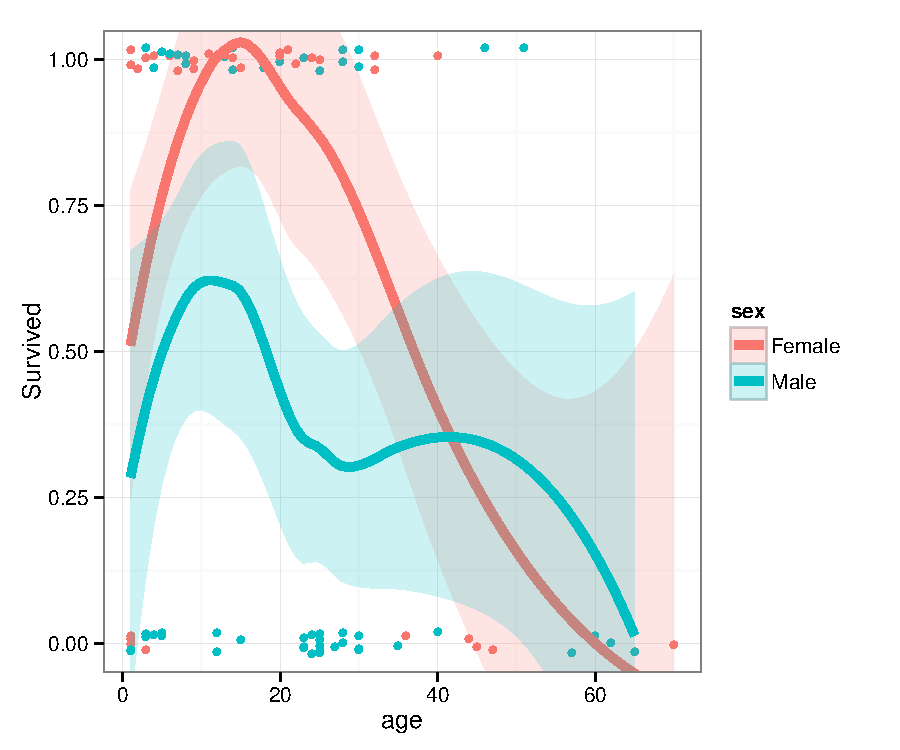
\includegraphics[width=.5\textwidth]{ch07/fig/donner1-cond3-2} }

\caption[Conditionals plot of the Donner data, showing the relationship of survival to age and sex]{Conditionals plot of the Donner data, showing the relationship of survival to age and sex. Left: The smoothed curves and confidence bands show the result of fitting separate quadratic logistic regressions on age for males and females. Right: Separate loess smooths are fit to the data for males and females\label{fig:donner1-cond3}}
\end{figure}


\end{knitrout}
This plot is quite surprising.  It suggests quite different regimes relating to survival
for men and women.  Among men, survival probability decreases steadily with age, at
least after age 20.  For women, those in the age range 10--35 were very likely to have
lived, while those over 40 were almost all predicted to perish.

Another simple technique is to fit a non-parametric loess smooth, as shown in the
right panel of \figref{fig:donner1-cond3}.  The curve for females is similar
to that of the quadratic fit in the left panel, but the curve for males
suggests that survival also has a peak around the teenage years.
One lesson to be drawn from these graphs is that a linear logistic regression,
such as shown in \figref{fig:donner1-cond3} may tell only part of the story,
and, for a binary response it is not easy to discern whether the true
relationship is linear.  If it really is, all these graphs would look much
more similar.  As well, we usually obtain a more realistic smoothing of
the data using full-model plots or effect plots.


The suggestions from these exploratory graphs can be used to define and test some models
for survival in the Donner Party.  The substantive questions of interest are:
\begin{itemize}
  \item Is relationship the same for men and women?  This is, is it necessary to allow for an interaction of age with sex, or separate fitted curves for men and women?
  \item Is the relationship between survival and age well-represented in a linear logistic regression model?
\end{itemize}

The first question is the easiest to deal with:  we can simply fit a model allowing an
interaction of age (or some function of age) and sex,
\begin{verbatim}
survived ~ age * sex
survived ~ f(age) * sex
\end{verbatim}
and compare the goodness of fit with the analogous additive, main-effects models.

From a modeling perspective, there is a wide variety of approaches for testing for non-linear
relationships. We only scratch the surface here, and only for a single quantitative predictor,
$x$, such as age in this example.
One simple approach, illustrated in \figref{fig:donner1-cond3} is to allow a quadratic
(or higher-power, e.g., cubic) function to describe the relationship between the log odds
and $x$,

\begin{eqnarray*}
 \logit (\pi_i) & = & \alpha + \beta_1 x_i + \beta_2 x_i^2 \\
 \logit (\pi_i) & = & \alpha + \beta_1 x_i + \beta_2 x_i^2  + \beta_3 x_i^3 \\
 \dots
\end{eqnarray*}
In \R, these model terms can be fit using \code{poly(x, 2)}, \code{poly(x, 3)} $\dots$,
which generate orthogonal polynomials for the powers of $x$.  
A simple way to test for non-linearity is a likelihood ratio test comparing the
more complex model to the linear one.  This method is often sufficient for a hypothesis
test, and, if the relationship truly is linear, the fitted logits and probabilities
will not differ greatly from what they would be under a linear model.
A difficulty with this approach is that polynomial models are often unrealistic,
particularly for data that approach an asymptote.

Another  simple approach is to use a \term{regression spline},
that fits the relationship with $x$ in terms of a set of piecewise
polynomials, usually cubic, joined at a collection of points, called \emph{knots}
so that the overall fitted relationship is smooth and continuous.
See \citet[\S 17.2]{Fox:2008} for a cogent, brief description of these methods.

One particularly convenient method is a \term{natural spline}, implemented
in the \Rpackage{splines} in the \func{ns} function. This method constrains the
fitted cubic spline to be linear at lower and upper limits of $x$,
and, for $k$ knots, fits $\textrm{df} = k+1$ parameters not counting the intercept.
The $k$ knots can be conveniently chosen as $k$ cutpoints in the percentiles
of the distribution of $x$.  For example, with $k=1$, the knot would be placed
at the median, or 50th percentile; with $k=3$, the knots would be placed at the
quartiles of the distribution of $x$; $k=0$ corresponds to no knots, i.e.,
a simple linear regression.

In the \func{ns} function, you can specify the locations of knots or the number of knots
with the \code{knots} argument, but it is conceptually simpler to specify the 
number of degrees of freedom used in the spline fit. Thus, 
\code{ns(x, 2)} and \code{poly(x, 2)} both specify a term in \code{x} of the same
complexity, the former a natural spline with $k=1$ knot and the later
a quadratic function in \code{x}.

We illustrate these ideas in the remainder of this example, fitting a
$2 \times 2$ collection of models to the \data{Donner} data
corresponding to:
\begin{seriate}
 \item whether or not age and sex effects are additive;
 \item whether the effect is linear on the logit scale or non-linear (quadratic, here).
\end{seriate}
A brief summary of each model is given using the \func{Anova} in
the \Rpackage{car}, providing Type II tests of each effect.
As usual, \func{summary} would give more detailed output, including
tests for individual coefficients.
First, we fit the linear models, without and with an interaction term:
\begin{knitrout}
\definecolor{shadecolor}{rgb}{1, 0.961, 0.933}\color{fgcolor}\begin{kframe}
\begin{alltt}
\hlstd{donner.mod1} \hlkwb{<-} \hlkwd{glm}\hlstd{(survived} \hlopt{~} \hlstd{age} \hlopt{+} \hlstd{sex,}
                   \hlkwc{data}\hlstd{=Donner,} \hlkwc{family}\hlstd{=binomial)}
\hlkwd{Anova}\hlstd{(donner.mod1)}
\end{alltt}
\begin{verbatim}
## Analysis of Deviance Table (Type II tests)
## 
## Response: survived
##     LR Chisq Df Pr(>Chisq)   
## age     5.52  1     0.0188 * 
## sex     6.73  1     0.0095 **
## ---
## Signif. codes:  0 '***' 0.001 '**' 0.01 '*' 0.05 '.' 0.1 ' ' 1
\end{verbatim}
\begin{alltt}
\hlstd{donner.mod2} \hlkwb{<-} \hlkwd{glm}\hlstd{(survived} \hlopt{~} \hlstd{age} \hlopt{*} \hlstd{sex,}
                   \hlkwc{data}\hlstd{=Donner,} \hlkwc{family}\hlstd{=binomial)}
\hlkwd{Anova}\hlstd{(donner.mod2)}
\end{alltt}
\begin{verbatim}
## Analysis of Deviance Table (Type II tests)
## 
## Response: survived
##         LR Chisq Df Pr(>Chisq)   
## age         5.52  1     0.0188 * 
## sex         6.73  1     0.0095 **
## age:sex     0.40  1     0.5269   
## ---
## Signif. codes:  0 '***' 0.001 '**' 0.01 '*' 0.05 '.' 0.1 ' ' 1
\end{verbatim}
\end{kframe}
\end{knitrout}
\noindent The main effects of \var{age} and \var{sex} are both significant here,
but the interaction term, \code{age:sex} is not in model \code{donner.mod2}.


Next, we fit non-linear models, representing the linear and non-linear
trends in age by \code{poly(age,2)}.  Alternatively, we could use
the term \code{ns(age,2)} or higher-degree polynomials or 
natural splines with more knots, but we don't do this here.
\begin{knitrout}
\definecolor{shadecolor}{rgb}{1, 0.961, 0.933}\color{fgcolor}\begin{kframe}
\begin{alltt}
\hlstd{donner.mod3} \hlkwb{<-} \hlkwd{glm}\hlstd{(survived} \hlopt{~} \hlkwd{poly}\hlstd{(age,}\hlnum{2}\hlstd{)} \hlopt{+} \hlstd{sex,}
                   \hlkwc{data}\hlstd{=Donner,} \hlkwc{family}\hlstd{=binomial)}
\hlkwd{Anova}\hlstd{(donner.mod3)}
\end{alltt}
\begin{verbatim}
## Analysis of Deviance Table (Type II tests)
## 
## Response: survived
##              LR Chisq Df Pr(>Chisq)   
## poly(age, 2)     9.91  2     0.0070 **
## sex              8.09  1     0.0044 **
## ---
## Signif. codes:  0 '***' 0.001 '**' 0.01 '*' 0.05 '.' 0.1 ' ' 1
\end{verbatim}
\begin{alltt}
\hlstd{donner.mod4} \hlkwb{<-} \hlkwd{glm}\hlstd{(survived} \hlopt{~} \hlkwd{poly}\hlstd{(age,}\hlnum{2}\hlstd{)} \hlopt{*} \hlstd{sex,}
                   \hlkwc{data}\hlstd{=Donner,} \hlkwc{family}\hlstd{=binomial)}
\hlkwd{Anova}\hlstd{(donner.mod4)}
\end{alltt}
\begin{verbatim}
## Analysis of Deviance Table (Type II tests)
## 
## Response: survived
##                  LR Chisq Df Pr(>Chisq)   
## poly(age, 2)         9.91  2     0.0070 **
## sex                  8.09  1     0.0044 **
## poly(age, 2):sex     8.93  2     0.0115 * 
## ---
## Signif. codes:  0 '***' 0.001 '**' 0.01 '*' 0.05 '.' 0.1 ' ' 1
\end{verbatim}
\end{kframe}
\end{knitrout}
\noindent Now, in model \code{donner.mod4},  the interaction term
\code{poly(age, 2):sex} is significant, indicating that the 
fitted quadratics for males and females differ in ``shape,''
meaning either their linear (slope) or quadratic (curvature)
components.

These four models address the questions posed earlier. A compact
summary of these models, giving the likelihood ratio tests
of goodness of fit, together with AIC and BIC statistics are
shown below, using the \func{Summarise} method in \pkg{vcdExtra}
for a list of \class{glm} models.

\begin{knitrout}
\definecolor{shadecolor}{rgb}{1, 0.961, 0.933}\color{fgcolor}\begin{kframe}
\begin{alltt}
\hlkwd{library}\hlstd{(vcdExtra)}
\hlkwd{Summarise}\hlstd{(donner.mod1, donner.mod2, donner.mod3, donner.mod4)}
\end{alltt}
\begin{verbatim}
## Likelihood summary table:
##             AIC BIC LR Chisq Df Pr(>Chisq)    
## donner.mod1 117 125    111.1  3     <2e-16 ***
## donner.mod2 119 129    110.7  4     <2e-16 ***
## donner.mod3 115 125    106.7  4     <2e-16 ***
## donner.mod4 110 125     97.8  6     <2e-16 ***
## ---
## Signif. codes:  0 '***' 0.001 '**' 0.01 '*' 0.05 '.' 0.1 ' ' 1
\end{verbatim}
\end{kframe}
\end{knitrout}

By AIC and BIC, \code{donner.mod4} is best, and it is also the
only model with a non-significant LR $\chisq$ (residual deviance). Because these
models comprise a $2 \times 2$ set of hypotheses, it is easier to
compare models by extracting the LR statistics and arranging these
in a table, together with the their row and column differences.
\TODO{Perhaps this should be a real table, showing also the df differences in rows and columns.}
\begin{knitrout}
\definecolor{shadecolor}{rgb}{1, 0.961, 0.933}\color{fgcolor}\begin{kframe}
\begin{alltt}
\hlstd{mods} \hlkwb{<-} \hlkwd{list}\hlstd{(donner.mod1, donner.mod2, donner.mod3, donner.mod4)}
\hlstd{LR} \hlkwb{<-} \hlkwd{sapply}\hlstd{(mods,} \hlkwa{function}\hlstd{(}\hlkwc{x}\hlstd{) x}\hlopt{$}\hlstd{deviance)}
\hlstd{LR} \hlkwb{<-} \hlkwd{matrix}\hlstd{(LR,} \hlnum{2}\hlstd{,} \hlnum{2}\hlstd{)}
\hlkwd{rownames}\hlstd{(LR)} \hlkwb{<-} \hlkwd{c}\hlstd{(}\hlstr{"additive"}\hlstd{,} \hlstr{"non-add"}\hlstd{)}
\hlkwd{colnames}\hlstd{(LR)} \hlkwb{<-} \hlkwd{c}\hlstd{(}\hlstr{"linear"}\hlstd{,} \hlstr{"non-lin"}\hlstd{)}
\hlstd{LR}\hlkwb{<-} \hlkwd{cbind}\hlstd{(LR,} \hlkwc{diff}\hlstd{= LR[,}\hlnum{1}\hlstd{]}\hlopt{-}\hlstd{LR[,}\hlnum{2}\hlstd{])}
\hlstd{LR} \hlkwb{<-} \hlkwd{rbind}\hlstd{(LR,} \hlkwc{diff}\hlstd{=} \hlkwd{c}\hlstd{(LR[}\hlnum{1}\hlstd{,}\hlnum{1}\hlopt{:}\hlnum{2}\hlstd{]}\hlopt{-}\hlstd{LR[}\hlnum{2}\hlstd{,}\hlnum{1}\hlopt{:}\hlnum{2}\hlstd{],}\hlnum{0}\hlstd{))}
\hlstd{LR}
\end{alltt}
\begin{verbatim}
##             linear  non-lin    diff
## additive 111.12750 106.7313  4.3962
## non-add  110.72718  97.7992 12.9280
## diff       0.40032   8.9321  0.0000
\end{verbatim}
\end{kframe}
\end{knitrout}

Thus, the answer to our questions seems to be that:
\begin{seriate}
 \item there is evidence that the relationship of survival to age differs
 for men and women in the Donner Party;
 \item these relationships are not well-described by a linear logistic
 regression.
\end{seriate}

For simplicity, we used a quadratic effect, \code{poly(age,2)}, to test for
non-linearity here.  An alternative test of the same complexity 
could use a regression spline, \code{ns(age,2)}, also with 2 degrees of
freedom for the main effect and interaction, or allow more knots.
To illustrate, we fit two natural spline modes models with 2 and 4 df,
and compare these with the quadratic model (\code{donner.mod4}),
all of which include the interaction of age and sex.

\begin{knitrout}
\definecolor{shadecolor}{rgb}{1, 0.961, 0.933}\color{fgcolor}\begin{kframe}
\begin{alltt}
\hlkwd{library}\hlstd{(splines)}
\hlstd{donner.mod5} \hlkwb{<-} \hlkwd{glm}\hlstd{(survived} \hlopt{~} \hlkwd{ns}\hlstd{(age,}\hlnum{2}\hlstd{)} \hlopt{*} \hlstd{sex,} \hlkwc{data}\hlstd{=Donner,}
                   \hlkwc{family}\hlstd{=binomial)}
\hlkwd{Anova}\hlstd{(donner.mod5)}
\end{alltt}
\begin{verbatim}
## Analysis of Deviance Table (Type II tests)
## 
## Response: survived
##                LR Chisq Df Pr(>Chisq)   
## ns(age, 2)         9.28  2     0.0097 **
## sex                7.98  1     0.0047 **
## ns(age, 2):sex     8.71  2     0.0129 * 
## ---
## Signif. codes:  0 '***' 0.001 '**' 0.01 '*' 0.05 '.' 0.1 ' ' 1
\end{verbatim}
\begin{alltt}
\hlstd{donner.mod6} \hlkwb{<-} \hlkwd{glm}\hlstd{(survived} \hlopt{~} \hlkwd{ns}\hlstd{(age,}\hlnum{4}\hlstd{)} \hlopt{*} \hlstd{sex,} \hlkwc{data}\hlstd{=Donner,}
                   \hlkwc{family}\hlstd{=binomial)}
\hlkwd{Anova}\hlstd{(donner.mod6)}
\end{alltt}
\begin{verbatim}
## Analysis of Deviance Table (Type II tests)
## 
## Response: survived
##                LR Chisq Df Pr(>Chisq)    
## ns(age, 4)        22.05  4     0.0002 ***
## sex               10.49  1     0.0012 ** 
## ns(age, 4):sex     8.54  4     0.0737 .  
## ---
## Signif. codes:  0 '***' 0.001 '**' 0.01 '*' 0.05 '.' 0.1 ' ' 1
\end{verbatim}
\begin{alltt}
\hlkwd{Summarise}\hlstd{(donner.mod4, donner.mod5, donner.mod6)}
\end{alltt}
\begin{verbatim}
## Likelihood summary table:
##             AIC BIC LR Chisq Df Pr(>Chisq)    
## donner.mod4 110 125     97.8  6    < 2e-16 ***
## donner.mod5 111 126     98.7  6    < 2e-16 ***
## donner.mod6 106 131     86.1 10    3.2e-14 ***
## ---
## Signif. codes:  0 '***' 0.001 '**' 0.01 '*' 0.05 '.' 0.1 ' ' 1
\end{verbatim}
\end{kframe}
\end{knitrout}
With four more parameters, \code{donner.mod6} fits better and has
a smaller AIC.

We conclude this example with an effect plot for the spline model 
\code{donner.mod6} shown in \figref{fig:donner-effect}.
The complexity of the fitted relationships for men and women
is intermediate between the two conditional plots shown in 
\figref{fig:donner1-cond3}.  (However, note that the fitted effects are
plotted on the logit scale in \figref{fig:donner-effect} and labeled
with the corresponding probabilities, whereas the conditional plots
are plotted directly on the probability scale.)


\begin{knitrout}
\definecolor{shadecolor}{rgb}{1, 0.961, 0.933}\color{fgcolor}\begin{kframe}
\begin{alltt}
\hlkwd{library}\hlstd{(effects)}
\hlstd{donner.eff6} \hlkwb{<-} \hlkwd{allEffects}\hlstd{(donner.mod6,} \hlkwc{xlevels}\hlstd{=}\hlkwd{list}\hlstd{(}\hlkwc{age}\hlstd{=}\hlkwd{seq}\hlstd{(}\hlnum{0}\hlstd{,}\hlnum{50}\hlstd{,}\hlnum{5}\hlstd{)))}
\hlkwd{plot}\hlstd{(donner.eff6,} \hlkwc{ticks}\hlstd{=}\hlkwd{list}\hlstd{(}\hlkwc{at}\hlstd{=}\hlkwd{c}\hlstd{(}\hlnum{0.001}\hlstd{,} \hlnum{0.01}\hlstd{,} \hlnum{0.05}\hlstd{,} \hlnum{0.1}\hlstd{,} \hlnum{0.25}\hlstd{,}
                                  \hlnum{0.5}\hlstd{,} \hlnum{0.75}\hlstd{,} \hlnum{0.9}\hlstd{,} \hlnum{0.95}\hlstd{,} \hlnum{0.99}\hlstd{,} \hlnum{0.999}\hlstd{)))}
\end{alltt}
\end{kframe}\begin{figure}[!htbp]


\centerline{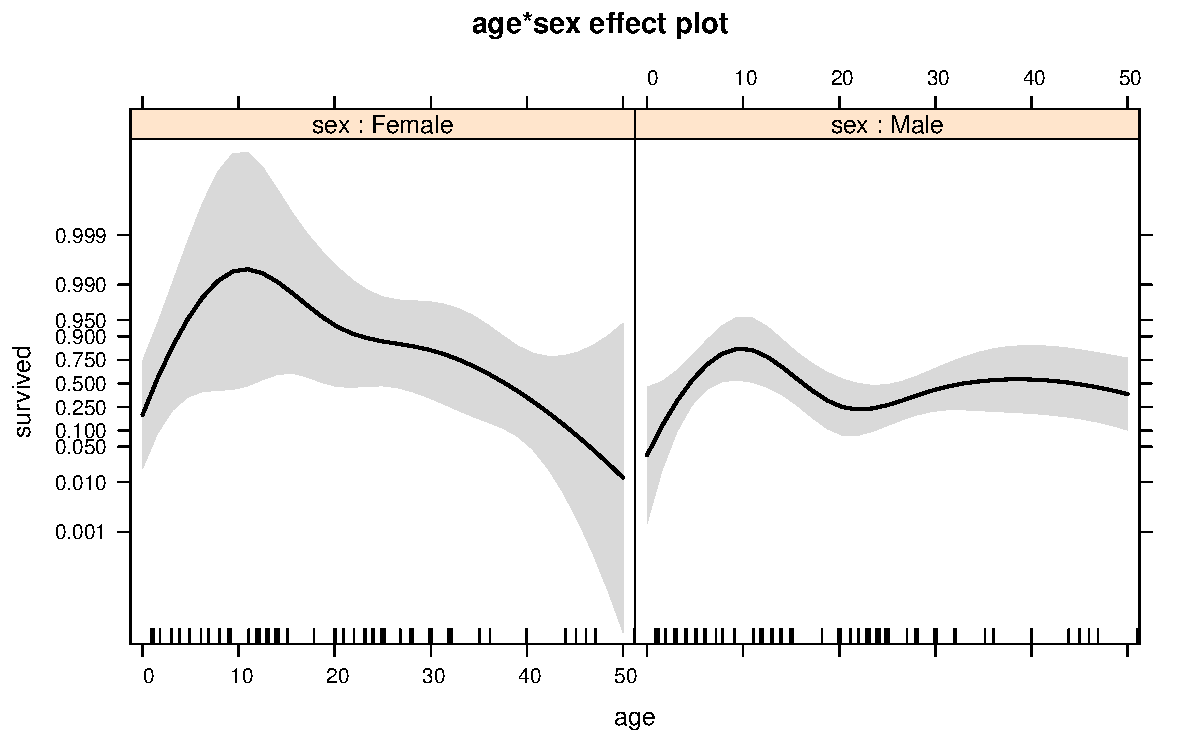
\includegraphics[width=.8\textwidth]{ch07/fig/donner-effect-1} }

\caption[Effect plot for the Donner data]{Effect plot for the Donner data\label{fig:donner-effect}}
\end{figure}


\end{knitrout}
This plot confirms that for women in the Donner Party, survival was greatest for
those aged 10-30.  Survival among men was overall much less and there is a 
hint of greater survival for men aged 10-15.

Of course, this statistical analysis does not provide explanations for these
effects, and it ignores the personal details of the Donner Party members and
the individual causes and circumstances of death, which are generally well-documented in the historical record \citep{Johnson:1996}.  See \url{http://user.xmission.com/~octa/DonnerParty/} for a comprehensive collection of historical sources.

\citet{Grayson:1990} attributes the greater survival of women of intermediate age to  
demographic arguments that women are overall better able to withstand conditions
of famine and extreme cold, and high age-specific mortality rates among the
youngest and oldest members of human societies.  He also concludes
(without much analysis) that members with larger social and kinship networks
would be more likely to survive.
\end{Example}

\begin{Example}[arrests]{Racial profiling: Arrests for marijuana possession}

In the summer of 2002, the \emph{Toronto Star} newspaper launched an investigation
on the topic of possible racial profiling by the Toronto police service.
Through freedom of information requests, they obtained a data base of over
600,000 arrest records on all potential charges in the period from 
1996--2002, the largest data bases on crime arrests and disposition 
ever assembled in Canada. An initial presentation of this study was given in \exref{ex:arrests0}.

In order to examine the issue of racial profiling (different treatment as a function of race)
they excluded all charges such as assault,
robbery, speeding and driving under the influence, where the police have
no discretion regarding the laying of a charge. They focused instead on 
a subset of arrests, where the police had various options.

Among these, for people arrested for a single charge of
simple possession of a small amount of marijuana, police have the
option of releasing the arrestee, with a summons (``Form 9'') to appear in court
(similar to a parking ticket), or else the person could be given
harsher treatment--brought to a police station or held in jail
for a bail hearing (``Show cause'').  The main question for the \emph{Toronto Star}
was whether the subject's skin color had any influence on the 
likelihood that the person would be released with a summons.%
\footnote{
Another discretionary charge they investigated was police stops for non-moving violations
under the Ontario \emph{Highway Traffic Act}, such as being pulled over
for a faulty muffler or having an expired license plate renewal sticker.
A disproportionate rate of charges against blacks is sometimes referred to
as ``driving while black'' (DWB). This investigation found that the number of blacks
so charged, but particularly young black males, far out-weighed their representation
in the population.
}

Their results, published in a week-long series of articles in December 2002,
concluded that there was strong evidence that black and white subjects were
treated differently. For example, the analysis showed that blacks were
1.5 times more likely than whites to be given harsher treatment than release
with a summons; if the subject was taken to the police station, a black was
1.6 times more likely to be held in jail for a bail hearing. An important
part of the analysis and the public debate that ensued was to show that
other variables that might account for these differences had been controlled
or adjusted for.%
\footnote{
The Toronto Police Service lauched a class-action libel
law suit against the \emph{Toronto Star} and the first author of this
book, who served as their statistical consultant, claiming damages of 
\$5,000 for every serving police officer in the city, a total of over
20 million dollars.  The suit was thrown out of court, and the Toronto
police took efforts to enhance training programs to combat the perception of racial profiling.
}

The data set \data{Arrests} in the \Rpackage{effects} gives a simplified version
of the \emph{Star} database, containing 
records for 5226 cases of arrest on the charge of simple
possession of marijhuana analyzed by the newspaper.
The response variable here is \var{released} (Yes/No)
and the main
predictor of interest is skin color of the person arrested, \var{colour}
(Black/White).%
\footnote{
The original data set also contained the categories Brown and Other,
but these appeared with small frequencies.
}
A random subset of the data set is shown below.

\begin{knitrout}
\definecolor{shadecolor}{rgb}{1, 0.961, 0.933}\color{fgcolor}\begin{kframe}
\begin{alltt}
\hlkwd{library}\hlstd{(effects)}
\hlkwd{data}\hlstd{(}\hlstr{"Arrests"}\hlstd{,} \hlkwc{package}\hlstd{=}\hlstr{"effects"}\hlstd{)}
\hlstd{Arrests[}\hlkwd{sample}\hlstd{(}\hlkwd{nrow}\hlstd{(Arrests),} \hlnum{6}\hlstd{),]}
\end{alltt}
\begin{verbatim}
##      released colour year age  sex employed citizen checks
## 3768      Yes  Black 2000  23 Male       No     Yes      4
## 4576      Yes  Black 2001  17 Male      Yes     Yes      0
## 3976       No  White 2002  20 Male       No     Yes      3
## 4629      Yes  White 2000  18 Male      Yes     Yes      1
## 2384       No  Black 2000  19 Male      Yes     Yes      3
## 869       Yes  White 2001  15 Male      Yes     Yes      1
\end{verbatim}
\end{kframe}
\end{knitrout}
Other available predictors, to be used as control variables included
the \var{year} of the arrest, \var{age} and \var{sex} of the person, and binary indicators
of whether the person was \var{employed} and a \var{citizen} of Canada.
In addition, when someone is stopped by police, his/her name is checked in six police
data bases that record previous arrests, convictions, whether on parole, etc.
The variable \var{checks} records the number, 0--6, in which the person's name
appeared.

A variety of logistic models were fit to these data including all possible main effects
and some two-way interactions. To allow for possible non-linear effects of \var{year},
this variable was treated as a factor rather than as a (linear) numeric variable,
but the effects of \var{age} and \var{checks} were reasonably linear on the logit scale.
A reasonable model included the interactions of \var{colour} with both \var{year} and
\var{age}, as fit below:

\begin{knitrout}
\definecolor{shadecolor}{rgb}{1, 0.961, 0.933}\color{fgcolor}\begin{kframe}
\begin{alltt}
\hlstd{Arrests}\hlopt{$}\hlstd{year} \hlkwb{<-} \hlkwd{as.factor}\hlstd{(Arrests}\hlopt{$}\hlstd{year)}
\hlstd{arrests.mod} \hlkwb{<-} \hlkwd{glm}\hlstd{(released} \hlopt{~} \hlstd{employed} \hlopt{+} \hlstd{citizen} \hlopt{+} \hlstd{checks}
                   \hlopt{+} \hlstd{colour}\hlopt{*}\hlstd{year} \hlopt{+} \hlstd{colour}\hlopt{*}\hlstd{age,}
                   \hlkwc{family}\hlstd{=binomial,} \hlkwc{data}\hlstd{=Arrests)}
\end{alltt}
\end{kframe}
\end{knitrout}
For such models, significance tests for the model terms are best carried out
using the \func{Anova} function in the \Rpackage{car} that uses Type II tests ...
\begin{knitrout}
\definecolor{shadecolor}{rgb}{1, 0.961, 0.933}\color{fgcolor}\begin{kframe}
\begin{alltt}
\hlkwd{library}\hlstd{(car)}
\hlkwd{Anova}\hlstd{(arrests.mod)}
\end{alltt}
\begin{verbatim}
## Analysis of Deviance Table (Type II tests)
## 
## Response: released
##             LR Chisq Df Pr(>Chisq)    
## employed        72.7  1    < 2e-16 ***
## citizen         25.8  1    3.8e-07 ***
## checks         205.2  1    < 2e-16 ***
## colour          19.6  1    9.7e-06 ***
## year             6.1  5    0.29785    
## age              0.5  1    0.49827    
## colour:year     21.7  5    0.00059 ***
## colour:age      13.9  1    0.00019 ***
## ---
## Signif. codes:  0 '***' 0.001 '**' 0.01 '*' 0.05 '.' 0.1 ' ' 1
\end{verbatim}
\end{kframe}
\end{knitrout}
The difficulty in interpreting these results from tables of coefficients can be seen
in the output below:
\begin{knitrout}\footnotesize
\definecolor{shadecolor}{rgb}{1, 0.961, 0.933}\color{fgcolor}\begin{kframe}
\begin{alltt}
\hlkwd{coeftest}\hlstd{(arrests.mod)}
\end{alltt}
\begin{verbatim}
## 
## z test of coefficients:
## 
##                      Estimate Std. Error z value Pr(>|z|)    
## (Intercept)           0.34443    0.31007    1.11  0.26665    
## employedYes           0.73506    0.08477    8.67  < 2e-16 ***
## citizenYes            0.58598    0.11377    5.15  2.6e-07 ***
## checks               -0.36664    0.02603  -14.08  < 2e-16 ***
## colourWhite           1.21252    0.34978    3.47  0.00053 ***
## year1998             -0.43118    0.26036   -1.66  0.09770 .  
## year1999             -0.09443    0.26154   -0.36  0.71805    
## year2000             -0.01090    0.25921   -0.04  0.96647    
## year2001              0.24306    0.26302    0.92  0.35541    
## year2002              0.21295    0.35328    0.60  0.54664    
## age                   0.02873    0.00862    3.33  0.00086 ***
## colourWhite:year1998  0.65196    0.31349    2.08  0.03756 *  
## colourWhite:year1999  0.15595    0.30704    0.51  0.61152    
## colourWhite:year2000  0.29575    0.30620    0.97  0.33411    
## colourWhite:year2001 -0.38054    0.30405   -1.25  0.21073    
## colourWhite:year2002 -0.61732    0.41926   -1.47  0.14091    
## colourWhite:age      -0.03737    0.01020   -3.66  0.00025 ***
## ---
## Signif. codes:  0 '***' 0.001 '**' 0.01 '*' 0.05 '.' 0.1 ' ' 1
\end{verbatim}
\end{kframe}
\end{knitrout}
By direct calculation (e.g., using \code{exp(coef(arrests.mod))}) you can find that
the odds of a quick release was $\exp({0.735})= 2.08$ times greater for someone employed,
$\exp({0.586})= 1.80$ times more likely for a Canadian citizen and 
$\exp({1.21})= 3.36$ times more likely for a white than a black person.
It is much more difficult to interpret the interaction terms.

The primary question for the newspaper concerned the overall difference between the 
the treatment of blacks and whites-- the main effect of \code{colour}.
We plot this as shown below, giving the plot shown in \figref{fig:arrests-eff1}.
This supports the claim by the \emph{Star} because the 95\% confidence limits for
blacks and whites do not overlap, and all other relevant predictors that could
account for this effect have been controlled or adjusted for.

\begin{knitrout}
\definecolor{shadecolor}{rgb}{1, 0.961, 0.933}\color{fgcolor}\begin{kframe}
\begin{alltt}
\hlkwd{plot}\hlstd{(}\hlkwd{Effect}\hlstd{(}\hlstr{"colour"}\hlstd{, arrests.mod),}
     \hlkwc{lwd}\hlstd{=}\hlnum{3}\hlstd{,} \hlkwc{ci.style}\hlstd{=}\hlstr{"bands"}\hlstd{,} \hlkwc{main}\hlstd{=}\hlstr{""}\hlstd{,}
     \hlkwc{xlab} \hlstd{=} \hlkwd{list}\hlstd{(}\hlstr{"Skin color of arrestee"}\hlstd{,} \hlkwc{cex}\hlstd{=}\hlnum{1.25}\hlstd{),}
     \hlkwc{ylab} \hlstd{=} \hlkwd{list}\hlstd{(}\hlstr{"Probability(released)"}\hlstd{,} \hlkwc{cex}\hlstd{=}\hlnum{1.25}\hlstd{)}
  \hlstd{)}
\end{alltt}
\end{kframe}\begin{figure}[!htbp]


\centerline{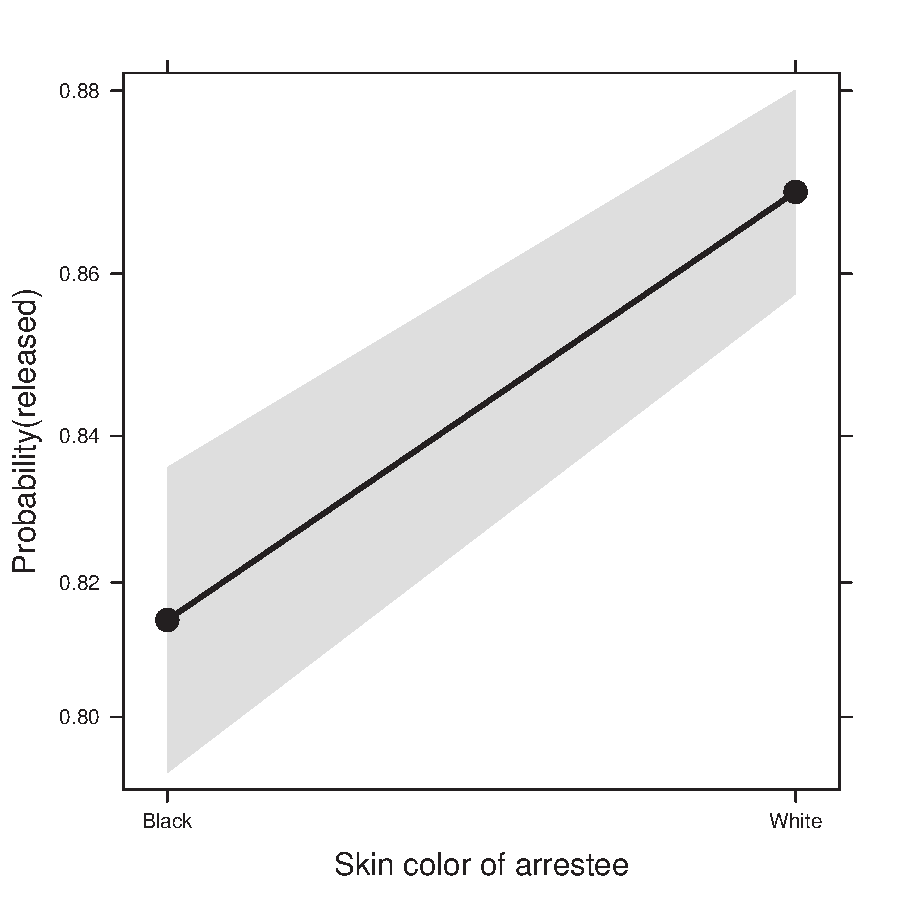
\includegraphics[width=.6\textwidth]{ch07/fig/arrests-eff1-1} }

\caption[Effect plot for the main effect of skin color in the Arrests data]{Effect plot for the main effect of skin color in the Arrests data.\label{fig:arrests-eff1}}
\end{figure}


\end{knitrout}

Of course, one should be very wary of interpreting main effects when there are
important interactions, and the story turned out to be far more nuanced than
was reported in the newspaper.  In particular, the interactions of color with
with age and year provided a more complete account.  Effect plots for these
interactions are shown in \figref{fig:arrests-eff2}.  

\begin{knitrout}
\definecolor{shadecolor}{rgb}{1, 0.961, 0.933}\color{fgcolor}\begin{kframe}
\begin{alltt}
\hlcom{# colour x age interaction}
\hlkwd{plot}\hlstd{(}\hlkwd{Effect}\hlstd{(}\hlkwd{c}\hlstd{(}\hlstr{"colour"}\hlstd{,}\hlstr{"age"}\hlstd{), arrests.mod),}
     \hlkwc{lwd}\hlstd{=}\hlnum{3}\hlstd{,} \hlkwc{multiline}\hlstd{=}\hlnum{TRUE}\hlstd{,}
     \hlkwc{xlab}\hlstd{=}\hlkwd{list}\hlstd{(}\hlstr{"Age"}\hlstd{,} \hlkwc{cex}\hlstd{=}\hlnum{1.25}\hlstd{),}
     \hlkwc{ylab}\hlstd{=}\hlkwd{list}\hlstd{(}\hlstr{"Probability(released)"}\hlstd{,} \hlkwc{cex}\hlstd{=}\hlnum{1.25}\hlstd{),}
     \hlkwc{key.args}\hlstd{=}\hlkwd{list}\hlstd{(}\hlkwc{x}\hlstd{=}\hlnum{.05}\hlstd{,} \hlkwc{y}\hlstd{=}\hlnum{.99}\hlstd{,} \hlkwc{cex}\hlstd{=}\hlnum{1.2}\hlstd{)}
     \hlstd{)}
\hlcom{# colour x year interaction}
\hlkwd{plot}\hlstd{(}\hlkwd{Effect}\hlstd{(}\hlkwd{c}\hlstd{(}\hlstr{"colour"}\hlstd{,}\hlstr{"year"}\hlstd{), arrests.mod),}
     \hlkwc{lwd}\hlstd{=}\hlnum{3}\hlstd{,} \hlkwc{multiline}\hlstd{=}\hlnum{TRUE}\hlstd{,}
     \hlkwc{xlab}\hlstd{=}\hlkwd{list}\hlstd{(}\hlstr{"Year"}\hlstd{,} \hlkwc{cex}\hlstd{=}\hlnum{1.25}\hlstd{),}
     \hlkwc{ylab}\hlstd{=}\hlkwd{list}\hlstd{(}\hlstr{"Probability(released)"}\hlstd{,} \hlkwc{cex}\hlstd{=}\hlnum{1.25}\hlstd{),}
     \hlkwc{key.args}\hlstd{=}\hlkwd{list}\hlstd{(}\hlkwc{x}\hlstd{=}\hlnum{.7}\hlstd{,} \hlkwc{y}\hlstd{=}\hlnum{.99}\hlstd{,} \hlkwc{cex}\hlstd{=}\hlnum{1.2}\hlstd{)}
     \hlstd{)}
\end{alltt}
\end{kframe}\begin{figure}[!htbp]


\centerline{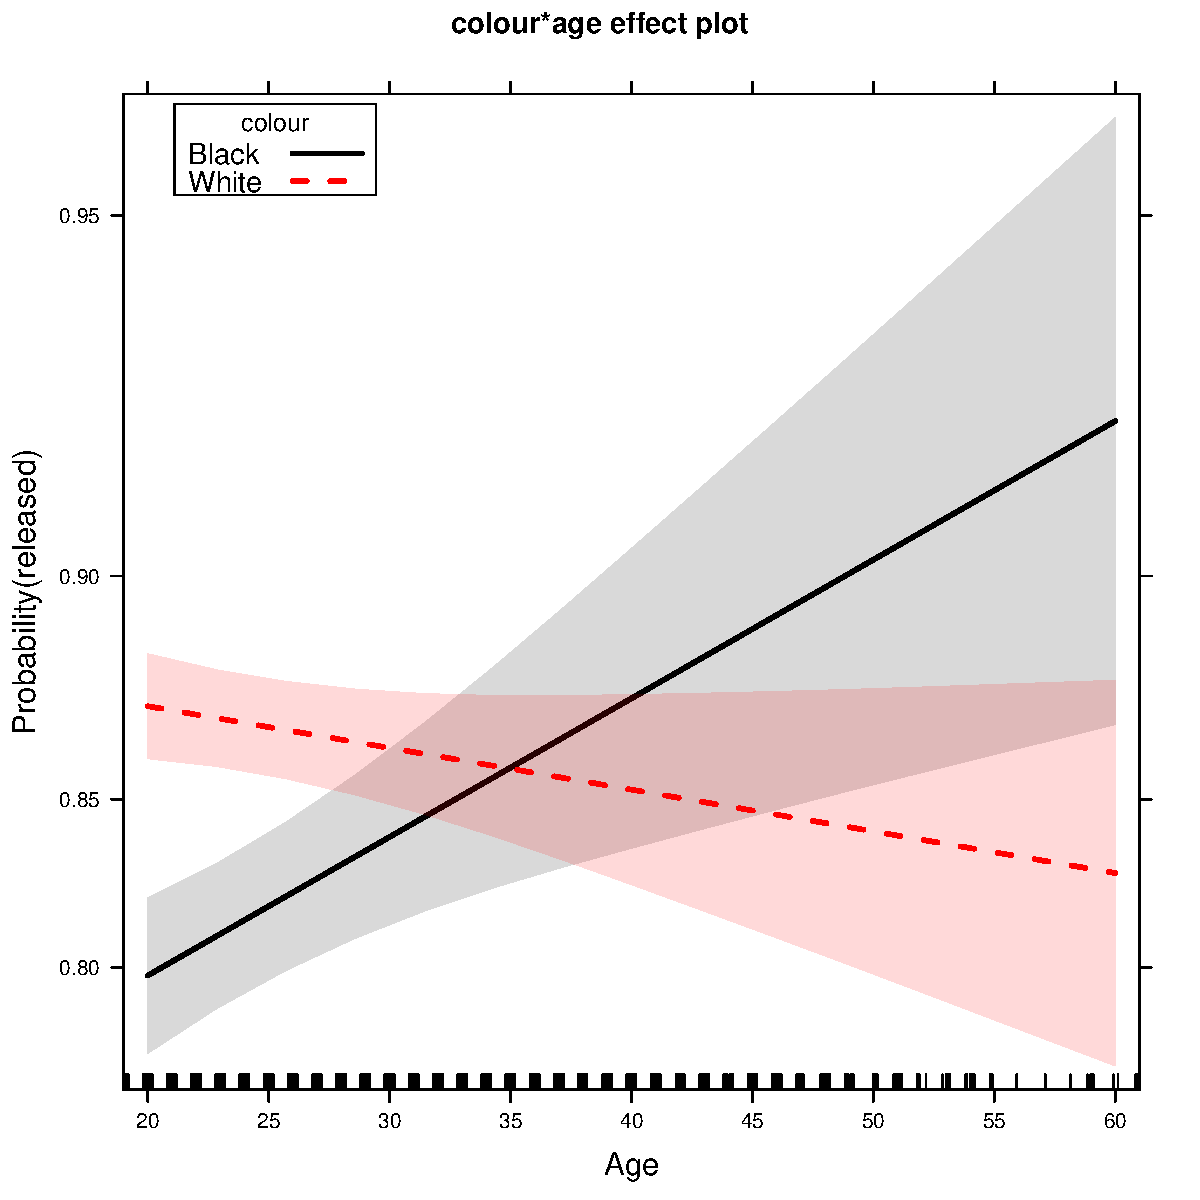
\includegraphics[width=.49\textwidth]{ch07/fig/arrests-eff2-1} 
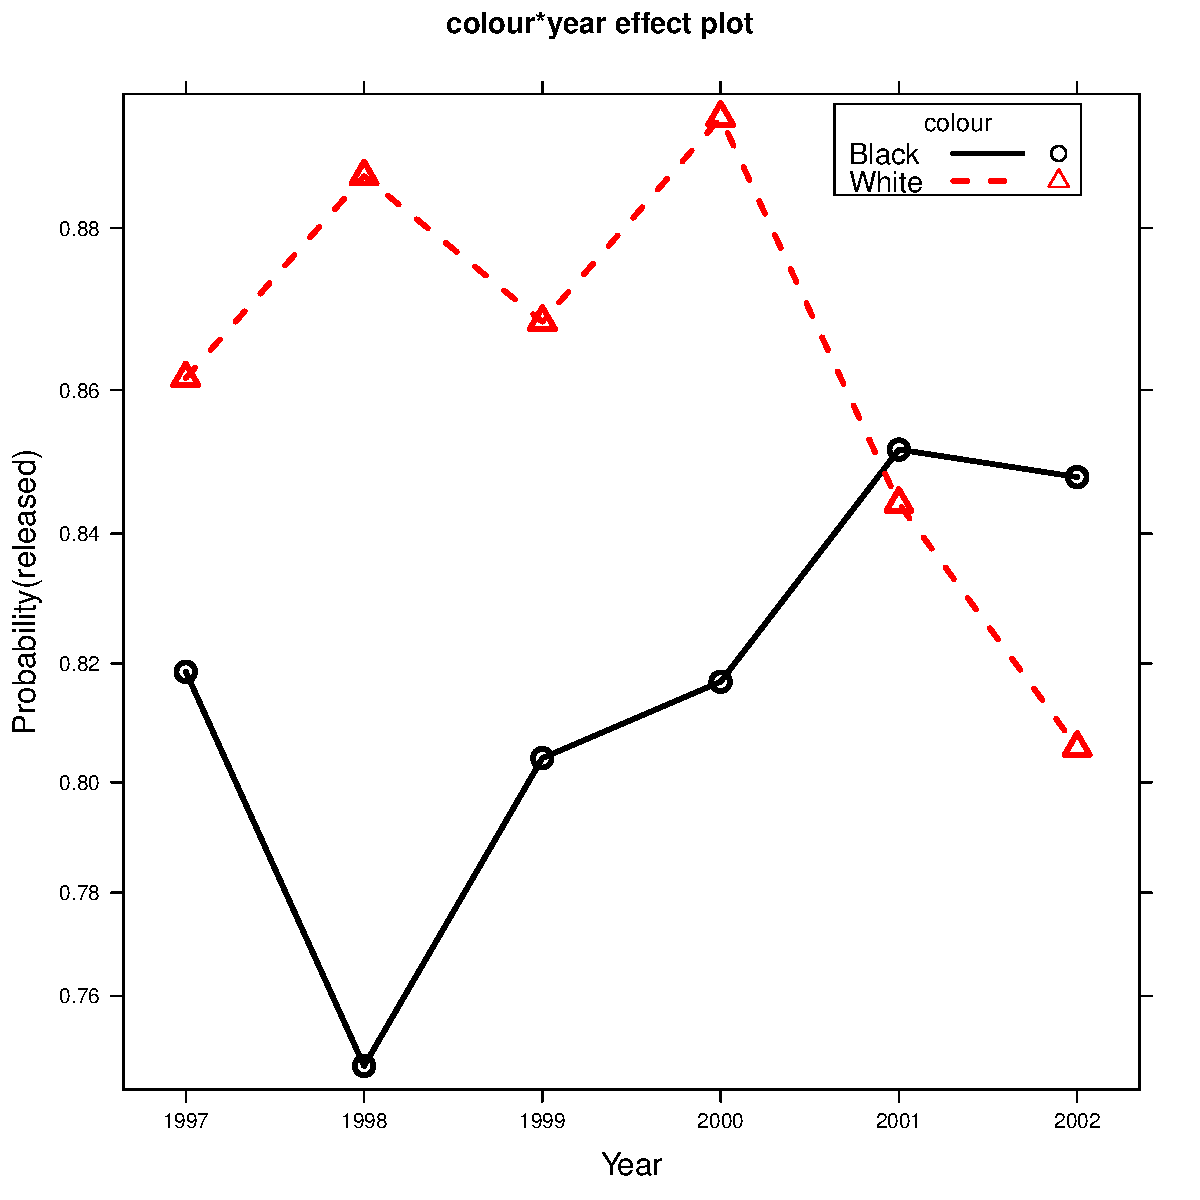
\includegraphics[width=.49\textwidth]{ch07/fig/arrests-eff2-2} }

\caption[Effect plots for the interactions of color with age (left) and year (right) in the Arrests data]{Effect plots for the interactions of color with age (left) and year (right) in the Arrests data.\label{fig:arrests-eff2}}
\end{figure}


\end{knitrout}
From the left panel in \figref{fig:arrests-eff2}, it is immediately apparent that
the effect of age was in opposite directions for blacks and whites:
Young blacks were indeed treated more severely than young whites; however
for older people, blacks were treated less harshly than whites,
controlling for all other predictors.

The right panel of \figref{fig:arrests-eff2} shows the changes over time in
the treatment of blacks and whites.  It can be seen that up to the year 2000
there was strong evidence for differential treatment on these charges,
again controlling for other predictors.  There was also evidence to support
the claim by the police that in the year 2001 they began training of officers
to reduce racial effects in treatment.

Finally, the \Rpackage{effects} provides a convenience function, \func{allEffects}, that
calculates the effects for all high-order terms in a given model. The \func{plot} method
for the \class{efflist} object can be used to plot individual terms selectively from
a graphic menu, or plot all terms together in one comprehensive display using
\code{ask=FALSE}.

\begin{knitrout}
\definecolor{shadecolor}{rgb}{1, 0.961, 0.933}\color{fgcolor}\begin{kframe}
\begin{alltt}
\hlstd{arrests.effects} \hlkwb{<-} \hlkwd{allEffects}\hlstd{(arrests.mod,}
                              \hlkwc{xlevels}\hlstd{=}\hlkwd{list}\hlstd{(}\hlkwc{age}\hlstd{=}\hlkwd{seq}\hlstd{(}\hlnum{15}\hlstd{,}\hlnum{45}\hlstd{,}\hlnum{5}\hlstd{)))}
\hlkwd{plot}\hlstd{(arrests.effects,}
     \hlkwc{ylab}\hlstd{=}\hlstr{"Probability(released)"}\hlstd{,} \hlkwc{ci.style}\hlstd{=}\hlstr{"bands"}\hlstd{,} \hlkwc{ask}\hlstd{=}\hlnum{FALSE}\hlstd{)}
\end{alltt}
\end{kframe}\begin{figure}[!htbp]


\centerline{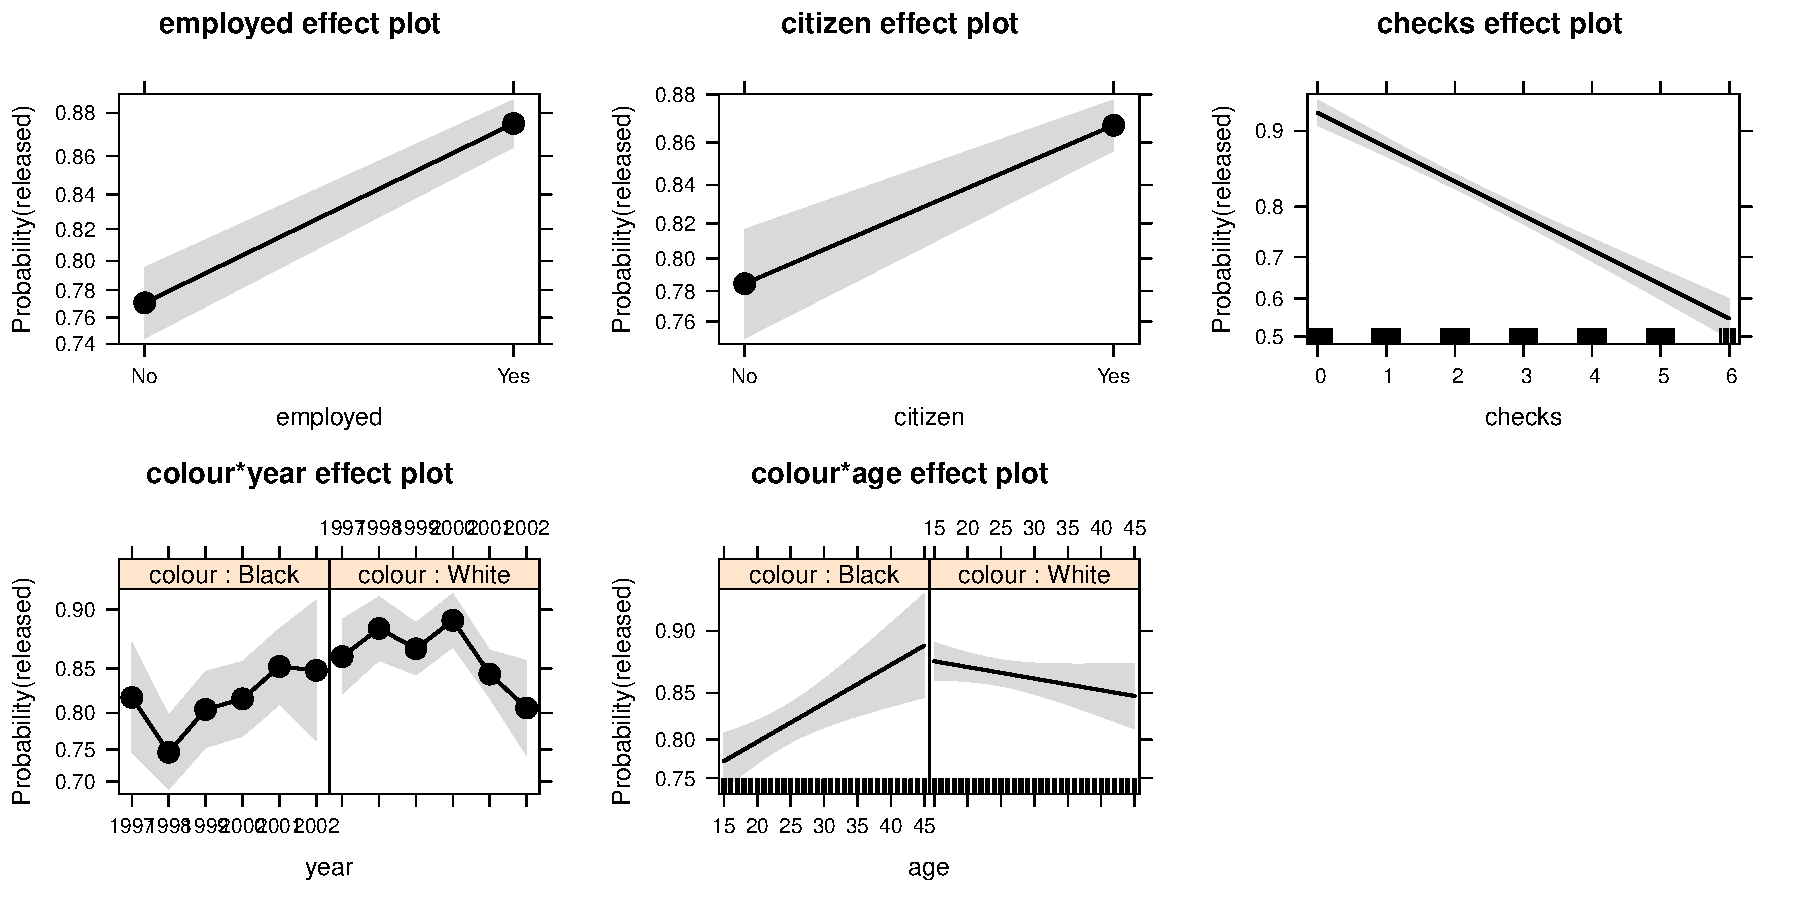
\includegraphics[width=\textwidth]{ch07/fig/arrests-all-1} }

\caption[Effect plot for all high-order terms in the model for the Arrests data]{Effect plot for all high-order terms in the model for the Arrests data\label{fig:arrests-all}}
\end{figure}


\end{knitrout}

The result, shown in \figref{fig:arrests-all} is a relatively compact and understandable
summary of the \code{arrests.mod} model:
\begin{seriate}
  \item people were more likely to be released if they were employed and citizens.
  \item each additional police check decreased the likelihod of release with a summons.
  \item the effect of skin color varied with age and year of arrest, in ways that
  tell a far more nuanced story than reported in the newspaper.
\end{seriate}

Finally, another feature of this plot bears mention:  by default, the scales for each
effect plot are determined separately for each effect, to maximize use of the plot region.
However, you have to read the $Y$ scale values to judge the relative sizes of these effects.
An alternative plot, using the \emph{same} scale in each subplot%
\footnote{
With the \Rpackage{effects}, you can set the \code{ylim} argument to equate the 
vertical range for all plots.  For this plot, \code{ylim = c(0.5, 1)} would work.
}
would show the relative sizes of these effects.

\end{Example}

\subsection{More complex models: Model selection and visualization}\label{sec:complex}

Models with more predictors or more complex terms (interactions, non-linear terms)
present additional challenges for model fitting, summarization,
and visualization and interpretation.
A very complicated model, with many terms and interactions may fit the data at hand
quite well. However, because goodness-of-fit is optimized in the sample, 
terms that appear significant are less likely to be important in a future sample,
and we need to worry about inflation of Type I error rates that accompany
multiple significance tests.  As well, it becomes increasingly difficult to
visualize and understand a fitted model as the model becomes increasingly complex.

On the other hand, a very simple model may omit important predictors, interactions, or
non-linear relationships with the response and give an illusion of a comfortable
interpretation.  

\TODO{Complete this brief introduction to model selection and define AIC/BIC,}


\begin{Example}[icu1]{Death in the ICU}

In this example we examine briefly some aspects of logistic regression
related to model selection and graphical display with a large collection
of potential predictors, including both 
quantitative and discrete variables.
We use data from a classic study by
\citet{Lemeshow-etal:88} of patients admitted to an intensive care unit at
Baystate Medical Center in Springfield,
Massachusetts.  The major goal of this study was to develop a 
model to predict the probability of survival (until hospital
discharge) of these patients and to study the risk factors associated with 
ICU mortality.
The data, contained in the data set \data{ICU} in \pkg{vcdExtra},
gives the results for a sample of 200 patients 
that was presented in \citet{HosmerLemeshowSturdivant:2013}
(and earlier editions).

The \data{ICU} contains 22 variables of which the first, \var{died}
is a factor.  Among the predictors, two variables (\var{race}, \var{coma})
were represented initially as 3-level factors, but then recoded to
binary variables (\var{white}, \var{uncons}).  
\begin{knitrout}
\definecolor{shadecolor}{rgb}{1, 0.961, 0.933}\color{fgcolor}\begin{kframe}
\begin{alltt}
\hlkwd{data}\hlstd{(}\hlstr{"ICU"}\hlstd{,} \hlkwc{package}\hlstd{=}\hlstr{"vcdExtra"}\hlstd{)}
\hlkwd{names}\hlstd{(ICU)}
\end{alltt}
\begin{verbatim}
##  [1] "died"     "age"      "sex"      "race"     "service" 
##  [6] "cancer"   "renal"    "infect"   "cpr"      "systolic"
## [11] "hrtrate"  "previcu"  "admit"    "fracture" "po2"     
## [16] "ph"       "pco"      "bic"      "creatin"  "coma"    
## [21] "white"    "uncons"
\end{verbatim}
\begin{alltt}
\hlstd{ICU} \hlkwb{<-} \hlstd{ICU[,}\hlopt{-}\hlkwd{c}\hlstd{(}\hlnum{4}\hlstd{,} \hlnum{20}\hlstd{)]}  \hlcom{# remove redundant race, coma}
\end{alltt}
\end{kframe}
\end{knitrout}
Removing the 3-level versions leaves 19 predictors, of which three
(age, heart rate, systolic blood pressure) are quantitative
and the remainder are either binary  (service, cancer) or had
previously been dichotomized (\code{ph<7.25}).

As an initial step, and a basis for comparison, we fit the full model
containing all 19 predictors.  
\begin{knitrout}
\definecolor{shadecolor}{rgb}{1, 0.961, 0.933}\color{fgcolor}\begin{kframe}
\begin{alltt}
\hlstd{icu.full} \hlkwb{<-} \hlkwd{glm}\hlstd{(died} \hlopt{~} \hlstd{.,} \hlkwc{data}\hlstd{=ICU,} \hlkwc{family}\hlstd{=binomial)}
\hlkwd{summary}\hlstd{(icu.full)}
\end{alltt}
\begin{verbatim}
## 
## Call:
## glm(formula = died ~ ., family = binomial, data = ICU)
## 
## Deviance Residuals: 
##     Min       1Q   Median       3Q      Max  
## -1.8040  -0.5606  -0.2044  -0.0863   2.9773  
## 
## Coefficients:
##                 Estimate Std. Error z value Pr(>|z|)    
## (Intercept)     -6.72670    2.38551   -2.82   0.0048 ** 
## age              0.05639    0.01862    3.03   0.0025 ** 
## sexMale          0.63973    0.53139    1.20   0.2286    
## serviceSurgical -0.67352    0.60190   -1.12   0.2631    
## cancerYes        3.10705    1.04585    2.97   0.0030 ** 
## renalYes        -0.03571    0.80165   -0.04   0.9645    
## infectYes       -0.20493    0.55319   -0.37   0.7110    
## cprYes           1.05348    1.00661    1.05   0.2953    
## systolic        -0.01547    0.00850   -1.82   0.0686 .  
## hrtrate         -0.00277    0.00961   -0.29   0.7732    
## previcuYes       1.13194    0.67145    1.69   0.0918 .  
## admitEmergency   3.07958    1.08158    2.85   0.0044 ** 
## fractureYes      1.41140    1.02971    1.37   0.1705    
## po2<=60          0.07382    0.85704    0.09   0.9314    
## ph<7.25          2.35408    1.20880    1.95   0.0515 .  
## pco>45          -3.01844    1.25345   -2.41   0.0160 *  
## bic<18          -0.70928    0.90978   -0.78   0.4356    
## creatin>2        0.29514    1.11693    0.26   0.7916    
## whiteNon-white   0.56573    0.92683    0.61   0.5416    
## unconsYes        5.23229    1.22630    4.27    2e-05 ***
## ---
## Signif. codes:  0 '***' 0.001 '**' 0.01 '*' 0.05 '.' 0.1 ' ' 1
## 
## (Dispersion parameter for binomial family taken to be 1)
## 
##     Null deviance: 200.16  on 199  degrees of freedom
## Residual deviance: 120.78  on 180  degrees of freedom
## AIC: 160.8
## 
## Number of Fisher Scoring iterations: 6
\end{verbatim}
\end{kframe}
\end{knitrout}
\noindent You can see that a few predictors are individually significant, but many are not.

However, it is useful to carry out a simultaneous
global test of $H_0 : \vec{\beta}=0$ that \emph{all} regression coefficients
are zero.  If this test is not significant, it makes little sense to use
selection methods to choose individually significant predictors.
For convenience, we define a
simple function, \func{LRtest}, to calculate the likelihood ratio test
from the model components.
\begin{knitrout}
\definecolor{shadecolor}{rgb}{1, 0.961, 0.933}\color{fgcolor}\begin{kframe}
\begin{alltt}
\hlstd{LRtest} \hlkwb{<-} \hlkwa{function}\hlstd{(}\hlkwc{model}\hlstd{)}
  \hlkwd{c}\hlstd{(}\hlkwc{LRchisq}\hlstd{=(model}\hlopt{$}\hlstd{null.deviance} \hlopt{-} \hlstd{model}\hlopt{$}\hlstd{deviance),}
    \hlkwc{df}\hlstd{=(model}\hlopt{$}\hlstd{df.null} \hlopt{-} \hlstd{model}\hlopt{$}\hlstd{df.residual))}

\hlstd{(LR} \hlkwb{<-} \hlkwd{LRtest}\hlstd{(icu.full))}
\end{alltt}
\begin{verbatim}
## LRchisq      df 
##  79.383  19.000
\end{verbatim}
\begin{alltt}
\hlstd{(pvalue}\hlkwb{=}\hlnum{1}\hlopt{-}\hlkwd{pchisq}\hlstd{(LR[}\hlnum{1}\hlstd{],LR[}\hlnum{2}\hlstd{]))}
\end{alltt}
\begin{verbatim}
##    LRchisq 
## 2.3754e-09
\end{verbatim}
\end{kframe}
\end{knitrout}

At this point, it is tempting to examine the output from \code{summary(icu.full)}
shown above and eliminate those predictors which fail significance at some
specified level such as the conventional $\alpha=0.05.$
This is generally a bad idea for many reasons.%
\footnote{
It ignores the facts of 
\begin{seriate}
\item an arbitrary cutoff value for significance,
\item the strong likelihood that chance features of the data or outliers influence the result,
\item problems of colinearity, etc.  
\end{seriate}
See \citet[\S 4.3]{Harrell:2001} for a useful discussion
of these issues.
}

A marginally better approach is to remove non-significant variables 
whose coefficients have signs that don't make sense
from the substance of the problem.
For example,
in the full model, both \code{renal} (history of chronic renal failure)
and \code{infect} (infection probable at ICU admission)
have negative signs, meaning that their presence \emph{decreases} the odds of
death.  We remove those variables using \func{update};  as expected they make
little difference.

\begin{knitrout}\footnotesize
\definecolor{shadecolor}{rgb}{1, 0.961, 0.933}\color{fgcolor}\begin{kframe}
\begin{alltt}
\hlstd{icu.full1} \hlkwb{<-} \hlkwd{update}\hlstd{(icu.full, .} \hlopt{~} \hlstd{.} \hlopt{-} \hlstd{renal} \hlopt{-} \hlstd{fracture)}
\hlkwd{anova}\hlstd{(icu.full1, icu.full,} \hlkwc{test}\hlstd{=}\hlstr{"Chisq"}\hlstd{)}
\end{alltt}
\begin{verbatim}
## Analysis of Deviance Table
## 
## Model 1: died ~ age + sex + service + cancer + infect + cpr + systolic + 
##     hrtrate + previcu + admit + po2 + ph + pco + bic + creatin + 
##     white + uncons
## Model 2: died ~ age + sex + service + cancer + renal + infect + cpr + 
##     systolic + hrtrate + previcu + admit + fracture + po2 + ph + 
##     pco + bic + creatin + white + uncons
##   Resid. Df Resid. Dev Df Deviance Pr(>Chi)
## 1       182        122                     
## 2       180        121  2      1.7     0.43
\end{verbatim}
\end{kframe}
\end{knitrout}

Before proceeding to consider model selection, it is useful to get a better
visual overview of the current model than is available from a table
of coefficients and significance tests.  
Some very useful \func{print}, \func{summary} and \func{plot}
methods are available in the \Rpackage{rsm}.
Unfortunately, these require that the logistic model is 
fitted with \func{lrm} in that package rather than with \func{glm}.
We pause here to refit the same model as \code{icu.full1} in order to
show a plot of odds ratios for the terms in this model.

\begin{knitrout}
\definecolor{shadecolor}{rgb}{1, 0.961, 0.933}\color{fgcolor}\begin{kframe}
\begin{alltt}
\hlkwd{library}\hlstd{(rms)}
\hlstd{dd} \hlkwb{<-} \hlkwd{datadist}\hlstd{(ICU[,}\hlopt{-}\hlnum{1}\hlstd{])}
\hlkwd{options}\hlstd{(}\hlkwc{datadist}\hlstd{=}\hlstr{"dd"}\hlstd{)}
\hlstd{icu.lrm1} \hlkwb{<-} \hlkwd{lrm}\hlstd{(died} \hlopt{~} \hlstd{.,} \hlkwc{data}\hlstd{=ICU)}
\hlstd{icu.lrm1} \hlkwb{<-} \hlkwd{update}\hlstd{(icu.lrm1, .} \hlopt{~} \hlstd{.} \hlopt{-} \hlstd{renal} \hlopt{-} \hlstd{fracture)}
\end{alltt}
\end{kframe}
\end{knitrout}
The \func{summary} method for \class{rms} objects produces a much more detailed
descriptive summary of a fitted model, and the \func{plot} method for that summary object
gives a sensible plot of the odds ratios for the model terms together with confidence
intervals, at levels (0.9, 0.95, 0.99) by default.  The following lines produce
\figref{fig:icu1-odds-ratios}.

% This plot done manually & cropped
% <<icu1-odds-ratios, h=8, w=6, out.width='.7\\textwidth', cap='Odds ratios for the terms in the model for the ICU data. Each line shows the odds ratio for a term, together with lines for 90, 95 and 99\\% confidence intervals in progressively darker shades.'>>=
% sum.lrm1 <- summary(icu.lrm1)
% plot(sum.lrm1, log=TRUE, main="Odds ratio for 'died'", cex=1.25,
%      col = rgb(0.1, 0.1, 0.8, alpha = c(0.3, 0.5, 0.8)))
% @
\begin{knitrout}
\definecolor{shadecolor}{rgb}{1, 0.961, 0.933}\color{fgcolor}\begin{kframe}
\begin{alltt}
\hlstd{sum.lrm1} \hlkwb{<-} \hlkwd{summary}\hlstd{(icu.lrm1)}
\hlkwd{plot}\hlstd{(sum.lrm1,} \hlkwc{log}\hlstd{=}\hlnum{TRUE}\hlstd{,} \hlkwc{main}\hlstd{=}\hlstr{"Odds ratio for 'died'"}\hlstd{,} \hlkwc{cex}\hlstd{=}\hlnum{1.25}\hlstd{,}
     \hlkwc{col} \hlstd{=} \hlkwd{rgb}\hlstd{(}\hlnum{0.1}\hlstd{,} \hlnum{0.1}\hlstd{,} \hlnum{0.8}\hlstd{,} \hlkwc{alpha} \hlstd{=} \hlkwd{c}\hlstd{(}\hlnum{0.3}\hlstd{,} \hlnum{0.5}\hlstd{,} \hlnum{0.8}\hlstd{)))}
\end{alltt}
\end{kframe}
\end{knitrout}


\begin{figure}[!htb]
 \centering
 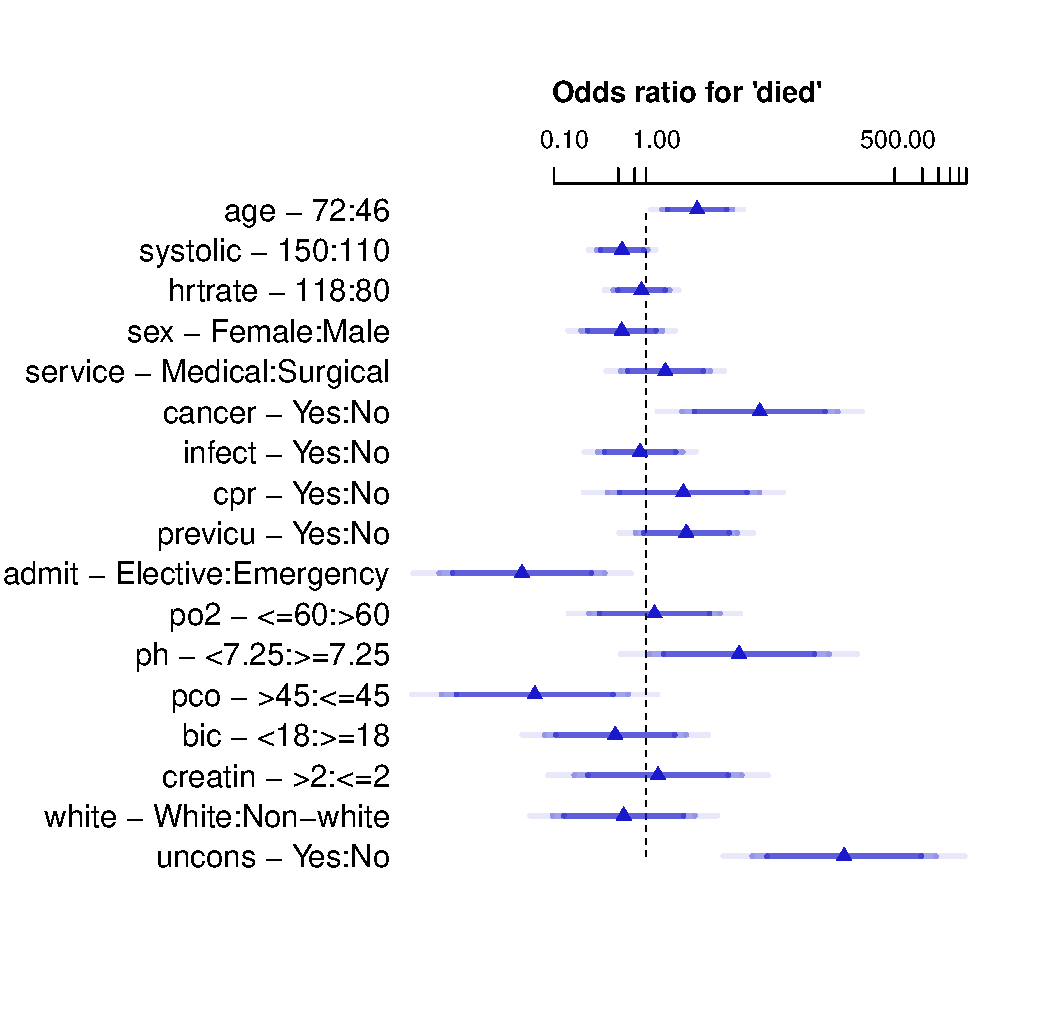
\includegraphics[width=.7\textwidth]{ch07/fig/icu-odds-ratios-cropped}
 \caption{Odds ratios for the terms in the model for the ICU data. Each line shows the odds ratio for a term, together with lines for 90, 95 and 99\% confidence intervals in progressively darker shades.}
 \label{fig:icu1-odds-ratios}
\end{figure}

In this plot, continuous variables are shown at the top, followed by the discrete predictors.
In each line, the range or levels of the predictors are given in the form $a:b$, such that
the value $a$ corresponds to the numerator of the odds ratio plotted.
Confidence intervals that don't overlap the vertical line for odds ratio = 1 are
significant, but this graph shows those at several confidence levels, allowing you to
decide what is ``signifcant'' visualy.  As well, the widths of those intervals
convey the precision of these estimates.

Among several stepwise selection methods in \R for \class{glm} models,
\func{stepAIC} in the \Rpackage{MASS} implements a reasonable collection
of methods for forward, backward and stepwise selection using penalized
AIC-like criteria that balance goodness of fit against parsimony.
The method takes an argument, \code{scope}, which is a list of
two model formulae; \code{upper} defines the largest (most complex)
model to consider and \code{lower} defines the smallest (simplest)
model, e.g., \verb|lower = ~ 1| is the intercept-only model.

By default, the function produces verbose printed output showing the details
of each step, but we suppress that here to save space.  It returns the final
model as its result, along with an \code{anova} component that summarises the
deviance and AIC from each step.
\begin{knitrout}
\definecolor{shadecolor}{rgb}{1, 0.961, 0.933}\color{fgcolor}\begin{kframe}
\begin{alltt}
\hlkwd{library}\hlstd{(MASS)}
\hlstd{icu.step1} \hlkwb{<-} \hlkwd{stepAIC}\hlstd{(icu.full1,} \hlkwc{trace} \hlstd{=} \hlnum{FALSE}\hlstd{)}
\hlstd{icu.step1}\hlopt{$}\hlstd{anova}
\end{alltt}
\begin{verbatim}
## Stepwise Model Path 
## Analysis of Deviance Table
## 
## Initial Model:
## died ~ age + sex + service + cancer + infect + cpr + systolic + 
##     hrtrate + previcu + admit + po2 + ph + pco + bic + creatin + 
##     white + uncons
## 
## Final Model:
## died ~ age + cancer + systolic + admit + ph + pco + uncons
## 
## 
##         Step Df Deviance Resid. Df Resid. Dev    AIC
## 1                              182     122.48 158.48
## 2      - po2  1 0.062446       183     122.54 156.54
## 3  - creatin  1 0.059080       184     122.60 154.60
## 4  - hrtrate  1 0.072371       185     122.67 152.67
## 5   - infect  1 0.122772       186     122.79 150.79
## 6    - white  1 0.334999       187     123.13 149.13
## 7  - service  1 0.671313       188     123.80 147.80
## 8      - bic  1 0.377521       189     124.18 146.18
## 9      - cpr  1 1.148260       190     125.33 145.33
## 10     - sex  1 1.543523       191     126.87 144.87
## 11 - previcu  1 1.569976       192     128.44 144.44
\end{verbatim}
\end{kframe}
\end{knitrout}

Alternatively, we can use the BIC criterion, by specifying \code{k}=$\log(n)$,
which generally will select a smaller model when the sample size is reasonably
large.
\begin{knitrout}
\definecolor{shadecolor}{rgb}{1, 0.961, 0.933}\color{fgcolor}\begin{kframe}
\begin{alltt}
\hlstd{icu.step2} \hlkwb{<-} \hlkwd{stepAIC}\hlstd{(icu.full,} \hlkwc{trace} \hlstd{=} \hlnum{FALSE}\hlstd{,} \hlkwc{k}\hlstd{=}\hlkwd{log}\hlstd{(}\hlnum{200}\hlstd{))}
\hlstd{icu.step2}\hlopt{$}\hlstd{anova}
\end{alltt}
\begin{verbatim}
## Stepwise Model Path 
## Analysis of Deviance Table
## 
## Initial Model:
## died ~ age + sex + service + cancer + renal + infect + cpr + 
##     systolic + hrtrate + previcu + admit + fracture + po2 + ph + 
##     pco + bic + creatin + white + uncons
## 
## Final Model:
## died ~ age + cancer + admit + uncons
## 
## 
##          Step Df  Deviance Resid. Df Resid. Dev    AIC
## 1                                180     120.78 226.74
## 2     - renal  1 0.0019881       181     120.78 221.45
## 3       - po2  1 0.0067968       182     120.79 216.16
## 4   - creatin  1 0.0621463       183     120.85 210.92
## 5   - hrtrate  1 0.0658870       184     120.92 205.69
## 6    - infect  1 0.2033221       185     121.12 200.59
## 7     - white  1 0.3673180       186     121.49 195.66
## 8       - bic  1 0.6002993       187     122.09 190.96
## 9   - service  1 0.7676303       188     122.85 186.43
## 10 - fracture  1 1.3245086       189     124.18 182.46
## 11      - cpr  1 1.1482598       190     125.33 178.31
## 12      - sex  1 1.5435228       191     126.87 174.55
## 13  - previcu  1 1.5699762       192     128.44 170.83
## 14       - ph  1 4.4412370       193     132.88 169.97
## 15      - pco  1 2.7302934       194     135.61 167.40
## 16 - systolic  1 3.5231028       195     139.13 165.63
\end{verbatim}
\end{kframe}
\end{knitrout}
This model differs from model \code{icu.step1} selected using AIC in the last
three steps, that also removed \var{ph}, \var{pco} and \var{systolic}.
\begin{knitrout}
\definecolor{shadecolor}{rgb}{1, 0.961, 0.933}\color{fgcolor}\begin{kframe}
\begin{alltt}
\hlkwd{coeftest}\hlstd{(icu.step2)}
\end{alltt}
\begin{verbatim}
## 
## z test of coefficients:
## 
##                Estimate Std. Error z value Pr(>|z|)    
## (Intercept)     -6.8698     1.3188   -5.21  1.9e-07 ***
## age              0.0372     0.0128    2.91  0.00360 ** 
## cancerYes        2.0971     0.8385    2.50  0.01238 *  
## admitEmergency   3.1022     0.9186    3.38  0.00073 ***
## unconsYes        3.7055     0.8765    4.23  2.4e-05 ***
## ---
## Signif. codes:  0 '***' 0.001 '**' 0.01 '*' 0.05 '.' 0.1 ' ' 1
\end{verbatim}
\end{kframe}
\end{knitrout}
These two models are nested, so we can compare them directly using a likelihood ratio
test from \func{anova}.
\begin{knitrout}
\definecolor{shadecolor}{rgb}{1, 0.961, 0.933}\color{fgcolor}\begin{kframe}
\begin{alltt}
\hlkwd{anova}\hlstd{(icu.step2, icu.step1,} \hlkwc{test}\hlstd{=}\hlstr{"Chisq"}\hlstd{)}
\end{alltt}
\begin{verbatim}
## Analysis of Deviance Table
## 
## Model 1: died ~ age + cancer + admit + uncons
## Model 2: died ~ age + cancer + systolic + admit + ph + pco + uncons
##   Resid. Df Resid. Dev Df Deviance Pr(>Chi)  
## 1       195        139                       
## 2       192        128  3     10.7    0.013 *
## ---
## Signif. codes:  0 '***' 0.001 '**' 0.01 '*' 0.05 '.' 0.1 ' ' 1
\end{verbatim}
\end{kframe}
\end{knitrout}
The larger model is significantly better by this test, but the smaller model is 
simpler to interpret. We retain these both as ``candidate models'' to be explored furth,
but for ease in this example, we do so using the smaller model, \code{icu.step2}.

Another important step is to check for non-linearity of quantitative predictors such
as \var{age} and interactions among the predictors.  This is easy to do using
\func{update} and \func{anova} as shown below.  First, allow a non-linear term
in \var{age}, and all two-way interactions of the binary predictors.
\begin{knitrout}
\definecolor{shadecolor}{rgb}{1, 0.961, 0.933}\color{fgcolor}\begin{kframe}
\begin{alltt}
\hlstd{icu.glm3} \hlkwb{<-} \hlkwd{update}\hlstd{(icu.step2, .} \hlopt{~} \hlstd{.} \hlopt{-}\hlstd{age} \hlopt{+} \hlkwd{ns}\hlstd{(age,}\hlnum{3}\hlstd{)} \hlopt{+} \hlstd{(cancer}\hlopt{+}\hlstd{admit}\hlopt{+}\hlstd{uncons)}\hlopt{^}\hlnum{2}\hlstd{)}
\hlkwd{anova}\hlstd{(icu.step2, icu.glm3,} \hlkwc{test}\hlstd{=}\hlstr{"Chisq"}\hlstd{)}
\end{alltt}
\begin{verbatim}
## Analysis of Deviance Table
## 
## Model 1: died ~ age + cancer + admit + uncons
## Model 2: died ~ cancer + admit + uncons + ns(age, 3) + cancer:admit + 
##     cancer:uncons + admit:uncons
##   Resid. Df Resid. Dev Df Deviance Pr(>Chi)
## 1       195        139                     
## 2       191        135  4     3.73     0.44
\end{verbatim}
\end{kframe}
\end{knitrout}
Next, we can check for interactions with \var{age}:
\begin{knitrout}
\definecolor{shadecolor}{rgb}{1, 0.961, 0.933}\color{fgcolor}\begin{kframe}
\begin{alltt}
\hlstd{icu.glm4} \hlkwb{<-} \hlkwd{update}\hlstd{(icu.step2, .} \hlopt{~} \hlstd{.} \hlopt{+} \hlstd{age}\hlopt{*}\hlstd{(cancer}\hlopt{+}\hlstd{admit}\hlopt{+}\hlstd{uncons))}
\hlkwd{anova}\hlstd{(icu.step2, icu.glm4,} \hlkwc{test}\hlstd{=}\hlstr{"Chisq"}\hlstd{)}
\end{alltt}
\begin{verbatim}
## Analysis of Deviance Table
## 
## Model 1: died ~ age + cancer + admit + uncons
## Model 2: died ~ age + cancer + admit + uncons + age:cancer + age:admit + 
##     age:uncons
##   Resid. Df Resid. Dev Df Deviance Pr(>Chi)
## 1       195        139                     
## 2       192        134  3     5.37     0.15
\end{verbatim}
\end{kframe}
\end{knitrout}
\noindent None of these additional terms have much effect.

So, we will tentatively adopt the simple main effects model, \code{icu.step2},
and consider how to visualize in interpret this result.
One interesting display is a \term{nomogram} that shows how values on the various
predictors translate into a predicted value of the log odds, and the relative
strengths of their effects on this prediction.  This kind of plot is shown in
\figref{fig:icu-nomogram}, produced using \func{nomogram} in the \Rpackage{rms}
as follows.  It only works with models fit using \func{lrm}, so we have to
refit this model.

\begin{knitrout}
\definecolor{shadecolor}{rgb}{1, 0.961, 0.933}\color{fgcolor}\begin{kframe}
\begin{alltt}
\hlstd{icu.lrm2} \hlkwb{<-} \hlkwd{lrm}\hlstd{(died} \hlopt{~} \hlstd{age} \hlopt{+} \hlstd{cancer}  \hlopt{+} \hlstd{admit} \hlopt{+} \hlstd{uncons,} \hlkwc{data}\hlstd{=ICU)}
\hlkwd{plot}\hlstd{(}\hlkwd{nomogram}\hlstd{(icu.lrm2),} \hlkwc{cex.var}\hlstd{=}\hlnum{1.2}\hlstd{,} \hlkwc{lplabel}\hlstd{=}\hlstr{"Log odds death"}\hlstd{)}
\end{alltt}
\end{kframe}
\end{knitrout}


\begin{figure}[!htb]
 \centering
 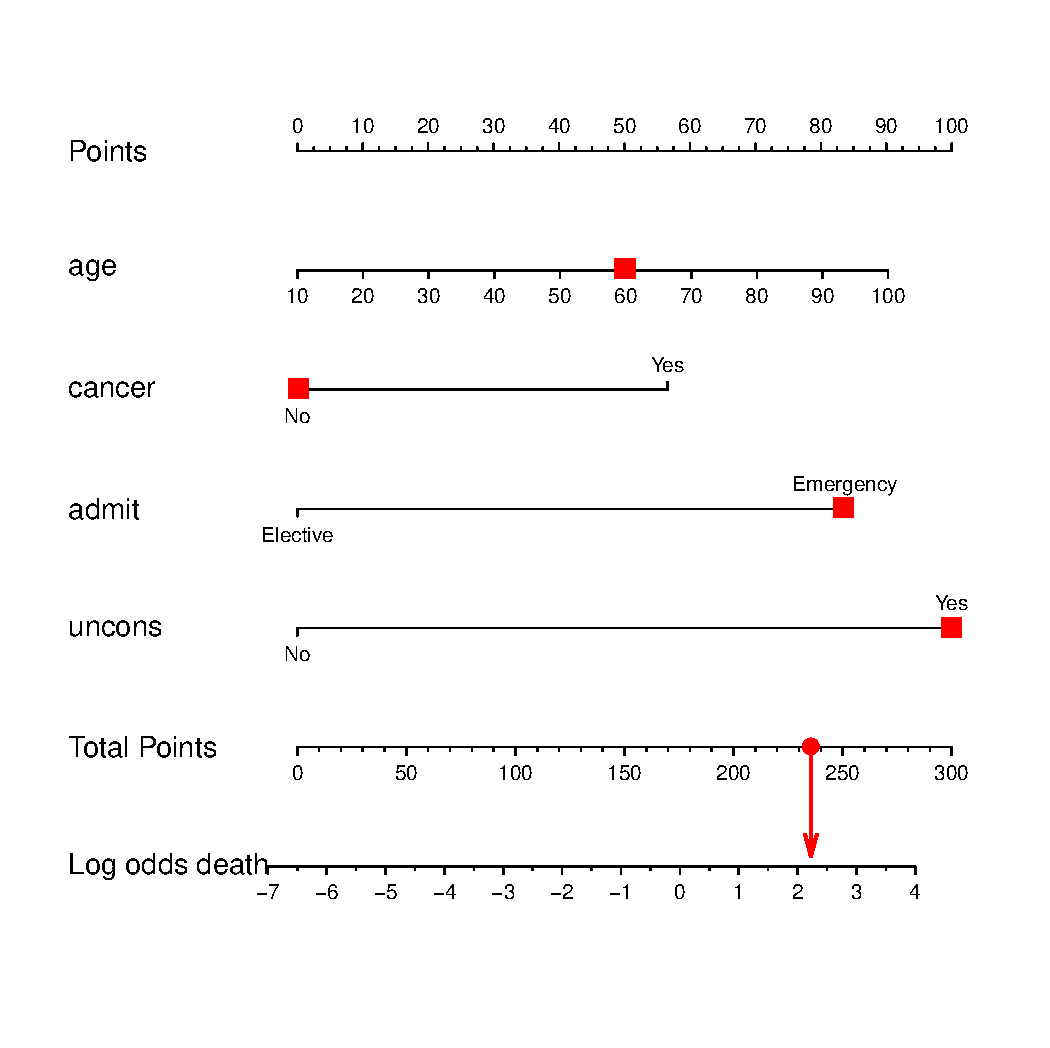
\includegraphics[width=.7\textwidth]{ch07/fig/icu-nomogram}
 \caption{Nomogram for predicted values in the simple main effects model for the ICU data.  Each predictor is scaled in relation to its effect on the outcome in terms of ``points'', 0--100.  Adding the points for a given case gives total points that have a direct translation to log odds.  The marked points show the prediction for someone of age 60, admitted to the emergency ward and unconscious. }
 \label{fig:icu-nomogram}
\end{figure}

In this nomogram, each predictor is scaled according to the size of its effect on a common scale
of 0--100 ``points.''  A representative observation is shown by the marked points, 
corresponding to a person of age 60, without cancer, who was admitted to emergency
and was unconscious at that time.  Adding the points associated with each variable
value gives the result shown on the scale of total points.
For this observation, the result is $50 + 0 + 84 +100 = 234$, for which the
scale of log odds at the bottom gives a predicted logit of 2.2, or a predicted 
probaility of death of $1/(1+\exp({-2.2}))= 0.90$.

This leaves us with the problem of how to visualize the fitted model compactly
and comprehensively.   Full-model plots and effect plots, as we have used them,
are somewhat unwieldly with four or more predictors if we want to view all
effects simultaneously because it is more difficult to make comparisons
across multiple panels (particularly if the vertical scales differ).

One way to reduce the visual complexity of such graphs is to combine some predictors
that would otherwise be shown in separate panels into a recoding that can be
shown as multiple curves for their combinations in fewer panels.  In general,
this can be done by combining some predictors interactively; for example
with sex and education as factors, their combinations, \code{M:Hi}, \code{M:Lo},
etc. could be used to define a new variable, \code{group} used as the curves
in one plot, rather than separate panels.

In this case, because age is continuous, it makes sense to plot fitted values
against age.  With \code{cancer},  \code{admit} and  \code{uncons} as binary
factors associated with risk of death, it is also sensible to combine them
all into a single variable, \code{risks}, indicating which one or more
risk factors are present for each case.  We first convert each variable
to an abbreviation for the risk, if present, or \code{""}, and paste
these together.

\begin{knitrout}\footnotesize
\definecolor{shadecolor}{rgb}{1, 0.961, 0.933}\color{fgcolor}\begin{kframe}
\begin{alltt}
\hlcom{# combine categorical risk factors to a single string}
\hlstd{risks} \hlkwb{<-} \hlstd{ICU[,} \hlkwd{c}\hlstd{(}\hlstr{"cancer"}\hlstd{,} \hlstr{"admit"}\hlstd{,} \hlstr{"uncons"}\hlstd{)]}
\hlstd{risks[,}\hlnum{1}\hlstd{]} \hlkwb{<-} \hlkwd{ifelse}\hlstd{(risks[,}\hlnum{1}\hlstd{]}\hlopt{==}\hlstr{"Yes"}\hlstd{,} \hlstr{"Cancer"}\hlstd{,} \hlstr{""}\hlstd{)}
\hlstd{risks[,}\hlnum{2}\hlstd{]} \hlkwb{<-} \hlkwd{ifelse}\hlstd{(risks[,}\hlnum{2}\hlstd{]}\hlopt{==}\hlstr{"Emergency"}\hlstd{,} \hlstr{"Emerg"}\hlstd{,} \hlstr{""}\hlstd{)}
\hlstd{risks[,}\hlnum{3}\hlstd{]} \hlkwb{<-} \hlkwd{ifelse}\hlstd{(risks[,}\hlnum{3}\hlstd{]}\hlopt{==}\hlstr{"Yes"}\hlstd{,} \hlstr{"Uncons"}\hlstd{,} \hlstr{""}\hlstd{)}
\hlstd{risks} \hlkwb{<-} \hlkwd{apply}\hlstd{(risks,} \hlnum{1}\hlstd{, paste,} \hlkwc{collapse}\hlstd{=}\hlstr{""}\hlstd{)}
\hlstd{risks[risks}\hlopt{==}\hlstr{""}\hlstd{]} \hlkwb{<-} \hlstr{"(none)"}
\end{alltt}
\end{kframe}
\end{knitrout}
\begin{knitrout}\footnotesize
\definecolor{shadecolor}{rgb}{1, 0.961, 0.933}\color{fgcolor}\begin{kframe}
\begin{alltt}
\hlkwd{table}\hlstd{(risks)}
\end{alltt}
\begin{verbatim}
## risks
##      (none)      Cancer CancerEmerg       Emerg EmergUncons 
##          37          15           5         128          14 
##      Uncons 
##           1
\end{verbatim}
\end{kframe}
\end{knitrout}
The frequency counts of the risk combinations show that admission to the
emergency ward alone was most frequent, and only one patient had
unconsciousness as the only risk.

As done before, we can then get the fitted logit values for the chosen model, 
and combine these with the data and the \code{risks} variable.

\begin{knitrout}
\definecolor{shadecolor}{rgb}{1, 0.961, 0.933}\color{fgcolor}\begin{kframe}
\begin{alltt}
\hlstd{icu.glm2} \hlkwb{<-} \hlkwd{glm}\hlstd{(died} \hlopt{~} \hlstd{age} \hlopt{+} \hlstd{cancer}  \hlopt{+} \hlstd{admit} \hlopt{+} \hlstd{uncons,}
                \hlkwc{data}\hlstd{=ICU,} \hlkwc{family}\hlstd{=binomial)}
\hlstd{icu.fit} \hlkwb{<-} \hlkwd{cbind}\hlstd{(ICU,} \hlkwd{predict}\hlstd{(icu.glm2,} \hlkwc{se}\hlstd{=}\hlnum{TRUE}\hlstd{), risks)}
\end{alltt}
\end{kframe}
\end{knitrout}

In the plot step below, we use \func{geom\_ribbon} to plot a one standard
error confidence band around the the fitted logits. \code{color=risks}
gives separate curves for each level of the risks factor.

\begin{knitrout}
\definecolor{shadecolor}{rgb}{1, 0.961, 0.933}\color{fgcolor}\begin{kframe}
\begin{alltt}
\hlstd{gg} \hlkwb{<-} \hlkwd{ggplot}\hlstd{( icu.fit,} \hlkwd{aes}\hlstd{(}\hlkwc{x}\hlstd{=age,} \hlkwc{y}\hlstd{=fit,} \hlkwc{color}\hlstd{=risks))} \hlopt{+}
  \hlkwd{geom_line}\hlstd{(}\hlkwc{size} \hlstd{=} \hlnum{1.2}\hlstd{)} \hlopt{+} \hlkwd{theme_bw}\hlstd{()} \hlopt{+}
  \hlkwd{geom_ribbon}\hlstd{(}\hlkwd{aes}\hlstd{(}\hlkwc{ymin} \hlstd{= fit} \hlopt{-} \hlstd{se.fit,}
                  \hlkwc{ymax} \hlstd{= fit} \hlopt{+} \hlstd{se.fit,}
                  \hlkwc{fill} \hlstd{= risks),}
              \hlkwc{alpha} \hlstd{=} \hlnum{0.2}\hlstd{,}
              \hlkwc{color} \hlstd{=} \hlstr{"transparent"}\hlstd{)} \hlopt{+}
  \hlkwd{theme_bw}\hlstd{()} \hlopt{+}
  \hlkwd{labs}\hlstd{(}\hlkwc{x} \hlstd{=} \hlstr{"Age"}\hlstd{,} \hlkwc{y} \hlstd{=} \hlstr{"Log odds (died)"}\hlstd{)} \hlopt{+}
  \hlkwd{geom_point}\hlstd{(}\hlkwc{size}\hlstd{=}\hlnum{2}\hlstd{)}
\end{alltt}
\end{kframe}
\end{knitrout}
By default, \func{ggplot} uses a legend to display the labels for the curve
variable, but the graph is more readable using \pkg{directlabels}, 
giving the plot shown in \figref{fig:icu1-fit-plot}.
\begin{knitrout}
\definecolor{shadecolor}{rgb}{1, 0.961, 0.933}\color{fgcolor}\begin{kframe}
\begin{alltt}
\hlkwd{library}\hlstd{(directlabels)}
\hlkwd{direct.label}\hlstd{(gg}\hlopt{+}\hlkwd{xlim}\hlstd{(}\hlnum{10}\hlstd{,}\hlnum{100}\hlstd{), last.points)}
\end{alltt}
\end{kframe}\begin{figure}[!htbp]


\centerline{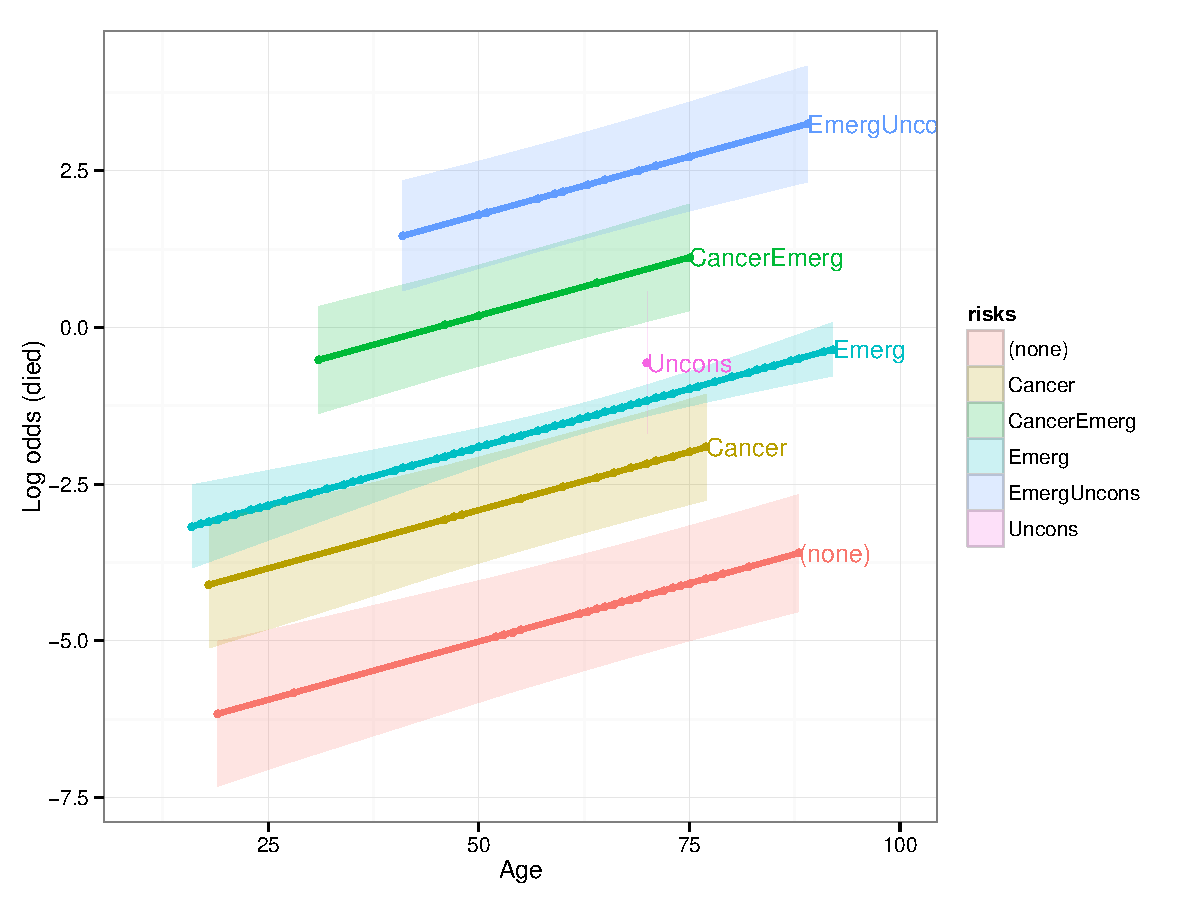
\includegraphics[width=.75\textwidth]{ch07/fig/icu1-fit-plot-1} }

\caption[Fitted log odds of death in the ICU data]{Fitted log odds of death in the ICU data. Each line shows the relationship with age, for patients having various combinations of risk factors.\label{fig:icu1-fit-plot}}
\end{figure}


\end{knitrout}
From this graph, it is apparent that the log odds of mortality increases with
age in all cases. Relative to the line labeled \code{(none)},
mortality is higher when any of these risk factors are present, particularly
when the patient is admitted to Emergency; it is highest when the
patient is also unconscious at admission.  The vertical gaps between lines
that share a common risk (e.g., \code{Cancer}, \code{CancerEmerg})
indicate the additional increment from one more risk.
Finally, the plotted points show the number and age distribution of
these various combinations.

Before concluding that this model provides an adequate description of the
data, we should examine whether any individual cases are unduly influencing
the predicted results, and more importantly, the choice of variables in
the model.  We examine this question in \secref{sec:logist-infl}
where we return to these data (\exref{ex:icu2}).

% The \Rpackage{rms} and its helper, \pkg{Hmisc} mask or modify functions in other packages, so it is best to detach them here.  \TODO{Maybe just do it and not say this.}


\end{Example}


\section{Influence and diagnostic plots}\label{sec:logist-infl}

In ordinary least squares (OLS) regression, measures of \term{influence}
(leverage, Cook's D, DFBETAs, etc.) and associated plots
help you to determine whether
individual cases (or cells in grouped data)
have undue impact on the fitted regression model and
the coefficients of individual predictors.
Analogs of most of these
measures have been suggested for logistic regression
and generalized linear models.
\citet{Pregibon:81} provided the theoretical basis for these methods,
exploiting the relationship between logistic models and
weighted least squares.  Some
additional problems occur in practical applications to
logistic regression because the response
is discrete, and because the leave-one-out diagnostics are more
difficult to compute, but the ideas are essentially the same.


\subsection{Residuals and leverage}\label{sec:logist-resids}
\ixon{logistic regression!residuals}
As in ordinary least squares regression, the influence (actual impact)
of an observation in logistic models depends multiplicatively
on its residual (disagreement between $y_i$ and $\hat{y}_i$)
and its leverage (how unusual $\vec{x}_i$ is in the space of the
explanatory variables).
A conceptual formula is
\begin{equation*}
  \mathrm{Influence} = \mathrm{Leverage} \times \mathrm{Residual}
\end{equation*}
This multiplicative definition implies that a case is influential to
the extent that it is both poorly fit \emph{and} has unusual values of
the predictors.

\subsubsection{Residuals}
In logistic regression, the simple raw residual is just $e_i \equiv y_i - \hat{p}_i$,
where 
%$ \hat{p}_i = \exp( \vec{x}_i\trans \vec{b} ) / [1 + \exp( \vec{x}_i\trans \vec{b} )]$.
$ \hat{p}_i = 1 / [1 + \exp(- \vec{x}_i\trans \vec{b} )]$.

The  Pearson and deviance residuals are more useful for identifying
poorly fitted observations, and are components of overall goodness-of-fit
statistics.
The (raw) \term{Pearson residual} is defined as
\begin{equation}\label{eq:reschi}
r_i \equiv \frac{e_i}{\sqrt{ p_i  (1-p_i)}}
\end{equation}
and the Pearson chi-square is therefore $\chisq = \sum r_i^2$.
The \term{deviance residual} is
\begin{equation}\label{eq:resdev}
g_i \equiv \pm { -2 [ y_i \log p_i  + (1-y_i) \log (1-p_i) ] }^{1/2}
\end{equation}
where the sign of $g_i$ is the same as that of $e_i$.
Likewise, the sum of squares of the deviance residuals gives
the overall deviance,
$G^2 = -2 \log \mathcal{L}(\vec{b}) = \sum g_i^2$.

When $y_i$ is a binomial count based on $n_i$ trials (grouped data),
the Pearson residuals \eqref{eq:reschi} then become
\begin{equation*}%\label{eq:reschi2}
r_i \equiv \frac{y_i -n_i p_i}{\sqrt{n_i  p_i  (1-p_i)}}
\end{equation*}
with similar modifications made to \eqref{eq:resdev}.

In \R, \func{residuals} is the generic function for obtaining (raw) residuals from
a model fitted with \func{glm} (or \func{lm}). However \term{standardized residuals},
\ix{residuals!standardized}
given by \func{rstandard}, and
 \term{studentized residuals},
\ix{residuals!studentized} 
provided by \func{rstudent} are often more useful
because they rescale the residuals to have unit variance.
They use, respectively, an overall estimate, $\hat{\sigma}^2$ of error variance, and the
leave-one-out estimate, $\hat{\sigma}_{(-i)}^2$, omitting the $i$th observation;
the studentized version is usually to be preferred in model diagnostics because
it also accounts for the impact of the observation on residual variance.

\ixoff{logistic regression!residuals}

\subsubsection{Leverage}
\ixon{logistic regression!leverage}
Leverage measures the \emph{potential} impact of an individual case
on the results, which is directly proportional to how far an
individual case is from the centroid in the space of the
predictors.  Leverage is defined as the diagonal elements,
\(h_{ii}\), of the ``Hat'' matrix, \(\mat{H}\),
\begin{equation*}%\label{eq:}
\mat{H} = {\mat{X}}^\star
{( {\mat{X}^\star}\trans {\mat{X}}^\star )}^{-1} {\mat{X}^\star}\trans
\end{equation*}
where \({\mat{X}} ^\star = {\mat{V}}^{1/2} \mat{X}\), and \(\mat{V}  =
\diag [ \hat{\vec{p}} ( 1 - \hat{\vec{p}})] \).  As in OLS,
leverage values are between 0 and 1, and a leverage value,
\(h_{ii}  > \{2 \mbox{ or } 3 \} k /  n\) is considered ``large''; here, \(k=p+1\) is the
number of coefficients including the intercept and \(n\) is the number of cases. 
In OLS, however, the hat values depend only on the $X$s, whereas
in logistic regression, they also depend on the dependent
variable values and the fitted probabilities (through $\mat{V}$).
As a result, an observation may be extremely unusual on the predictors,
yet not have a large hat value, if the fitted probability is near 0 or 1.
The function \func{hatvalues} calculates these values for a fitted
\class{glm} model object.
\ixoff{logistic regression!leverage}


\subsection{Influence diagnostics}\label{sec:logist-infldiag}

\ixon{logistic regression!influence diagnostics}
Influence measures assess the effect that deleting an
observation has on the regression parameters, fitted values, or the
goodness-of-fit statistics.  In OLS, these measures
can be computed exactly from a single regression.
In logistic regression, the exact effect of deletion
requires refitting the model with each observation deleted in turn,
%(because the estimating equations \eqref{eq:like4} are nonlinear),
a time-intensive computation.
Consequently, \citet{Pregibon:81} showed how analogous deletion
diagnostics may be approximated by performing one additional step
of the iterative procedure.  Most modern implementations of these
methods for generalized linear models follow \citet{Williams:87}.

The simplest measure of influence of observation $i$ is the standardized change in the coefficient for each variable due to omitting that observation,
termed \term{DFBETA}s.  From the relation \citep[p. 716]{Pregibon:81}
\begin{equation*}%\label{eq:dfbetas}
 \vec{b} -  \vec{b}_{(-i)} = (\mat{X}\trans \mat{V} \mat{X})^{-1} \vec{x}_i (y_i - p_i) / (1 - h_{ii})
 \comma
\end{equation*}
the estimated standardized change in the coefficient for variable $j$ is
\begin{equation}\label{eq:dfbeta}
 \mbox{DFBETA}{ij} \equiv \frac{b_{(-i)j} -  b_j } {\hat{\sigma} (b_j)}
 \comma
\end{equation}
where $\hat{\sigma} (b_j)$ is the estimated standard error of $b_j$.
With $k$ regressors, there are $k+1$ sets of DFBETAs, which makes their examination burdensome.
Graphical displays ease this burden, as do various summary measures
considered below.

The most widely used summary of the
overall influence of observation $i$ on the estimated regression
coefficients is \term{Cook's distance}, which measures
the average squared distance between $\vec{b}$ for all the data and
$\vec{b}_{(-i)}$ estimated without observation $i$.
It is defined as 
\begin{equation*}%\label{eq:cookd1}
C_i \equiv ( \vec{b} - \vec{b}_{(-i)} )\trans \:
    \mat{X}\trans \mat{V} \mat{X} \:
     ( \vec{b} - \vec{b}_{(-i)} ) / k \hat{\sigma}^2
    \period
\end{equation*}
However, \citet{Pregibon:81} showed that $C_i$ could be calculated
simply as
\begin{equation}\label{eq:cookd2}
 C_i = \frac{r_i^2 h_{ii}} {k (1-h_{ii} )^2}
 \comma
\end{equation}
where $r_i = y_i - \hat{p}_i / \sqrt{v_{ii} (1-h_{ii})}$ is the
$i$th standardized Pearson residual and $v_{ii}$ is the
$i$th diagonal element of $\mat{V}$.
Rules of thumb for noticeably ``large'' values of Cook's $D$ 
are only rough indicators, and designed so that only
``noteworthy'' observations are nominated as unusually influential.
One common cutoff for an observation to be treated as influential
is $C_i > 1$. Others refer the values of $C_i$ to a 
$\chisq_k$ or $F_{k, n-k}$ distribution.

Another commonly used summary statistic of overall influence is
the \term{DFFITS} statistic, a standardized measure of the difference
between the predicted value $\hat{y}_i$ using all the data
and the predicted value $\hat{y}_{(-i)}$ calculated omitting
the $i$th observation.
\begin{equation*}
\mbox{DFFITS}_i = \frac{\hat{y}_i - \hat{y}_{(-i)}} {\hat{\sigma}_{(-i)} \sqrt{h_{ii}}}
\comma
\end{equation*}
where $\hat{\sigma}_{(-i)}$ is the estimated standard error with the $i$th observation
deleted.  For computation, DFFITS can be expressed in terms of the standardized
Pearson residual and leverage as
\begin{equation}\label{eq:dffits}
\mbox{DFFITS}_i = r_i  \sqrt{ \frac{h_{ii}} {(1-h_{ii})} \frac{v_{ii}} {v_{(-ii)}} }
\period
\end{equation}
From \eqref{eq:cookd2} and \eqref{eq:dffits} it can be shown that Cook's distance is
nearly the square of DFFITS divided by $k$,
\begin{equation}\label{eq:cook-dffits}
C_i = \frac{v_{(-ii)}^2}{v_{ii}^2} \frac{\mbox{DFFITS}_i^2}{k}
\period
\end{equation}
Noteworthy values of DFFITS are often nominated by the rule-of-thumb
$\mbox{DFFITS}_i > 2 \mbox{ or } 3 \sqrt{k / n-k}$.

In \R, these influence measures are calculated for a fitted \class{glm}
model using \func{cooks.distance} and \func{dffits}.  
The \func{dfbeta} function calculates and returns the matrix of 
all standardized changes in the model coefficients (\eqref{eq:dfbeta})
due to omitting each observation in turn.%
\footnote{
\TODO{Not quite true:  \func{dfbeta} doesn't have a \class{glm} method.  Either omit
this or write a \func{dfbeta.glm} method that gives the same results as \func{influence.measures}.}
}
A convenience
function, \func{influence.measures} gives a tabular display showing
the $\mbox{DFBETA}_{ij}$ for each model variable, DFFITS, Cook's distances and the diagonal elements of the hat matrix. 
Cases which are influential with respect to any of these measures are marked with an asterisk.%
\footnote{
See \help{influence.measures} for the description of all of these functions for residuals,
leverage and influence diagnostics in generalized linear models.
}

Beyond printed output of these numerical summaries, plots of these measures can shed light
on potential problems due to influential or other noteworthy cases. By highlighting them,
such plots provide the opportunity to determine if and how any of these affect your 
conclusions, or to take some corrective action.

A basic collection of diagnostic plots is provided by the \func{plot} method for a 
\class{glm} model object. The \Rpackage{car} contains a variety of other functions
for model diagnostic plots.  We illustrate some of these in the examples below.

\ixoff{logistic regression!influence diagnostics}

% \begin{Example}[donner2]{Donner Party}
% \end{Example}

\begin{Example}[donner2]{Donner Party}
This example re-visits the data on the Donner Party examined in \exref{ex:donner1}.
For illustrative purposes, we consider the influence measures and diagnostic plots
for one specific model, the model \code{donner.mod3}, that included a 
quadratic effect of age and a main effect of sex, but no interaction.

The simplest overview of the adequacy of a fitted model is provided by the
\func{plot} method for a \class{glm} (or \class{lm}) object.
This function can produce up to six different plots that can be plotted individually
or selected (using the argument \code{which}) and composed into a single overview
figure using \code{par(mfrow=c(rows,cols))} as shown below. 

It is useful to see the entire collection because, by default, only four
are plotted (\code{which= c(1:3,5)}) and this selection 
(sometimes called the \term{regression quartet} of diagnostic plots)
is tuned more to classical
linear models for quantitative data.  Important feature of these plots are that
\begin{seriate}
 \item plot annotations are added to each showing trends or expected behaviour
 under the assumptions of a fitted model;
 \item noteworthy observations are labeled individually.
\end{seriate}

\begin{knitrout}
\definecolor{shadecolor}{rgb}{1, 0.961, 0.933}\color{fgcolor}\begin{kframe}
\begin{alltt}
\hlstd{caption} \hlkwb{=} \hlkwd{list}\hlstd{(}\hlstr{"(1) Residuals vs Fitted"}\hlstd{,}
               \hlstr{"(2) Normal Q-Q"}\hlstd{,}
               \hlstr{"(3) Scale-Location"}\hlstd{,}
               \hlstr{"(4) Cook's distance"}\hlstd{,}
               \hlstr{"(5) Residuals vs Leverage"}\hlstd{,}
               \hlkwd{expression}\hlstd{(}\hlstr{"(6) Cook's dist vs Leverage  "}
                          \hlopt{*} \hlstd{h[ii]} \hlopt{/} \hlstd{(}\hlnum{1} \hlopt{-} \hlstd{h[ii])))}
\hlstd{op} \hlkwb{<-} \hlkwd{par}\hlstd{(}\hlkwc{mfrow}\hlstd{=}\hlkwd{c}\hlstd{(}\hlnum{3}\hlstd{,}\hlnum{2}\hlstd{),} \hlkwc{mar}\hlstd{=}\hlkwd{c}\hlstd{(}\hlnum{4}\hlstd{,}\hlnum{4}\hlstd{,}\hlnum{2}\hlstd{,}\hlnum{1}\hlstd{)}\hlopt{+}\hlnum{.1}\hlstd{,} \hlkwc{cex.lab}\hlstd{=}\hlnum{1.2}\hlstd{,} \hlkwc{cex}\hlstd{=}\hlnum{1}\hlstd{)}
\hlkwd{plot}\hlstd{(donner.mod3,} \hlkwc{which}\hlstd{=}\hlnum{1}\hlopt{:}\hlnum{6}\hlstd{,} \hlkwc{caption}\hlstd{=caption)}
\hlkwd{par}\hlstd{(op)}
\end{alltt}
\end{kframe}\begin{figure}[!htbp]


\centerline{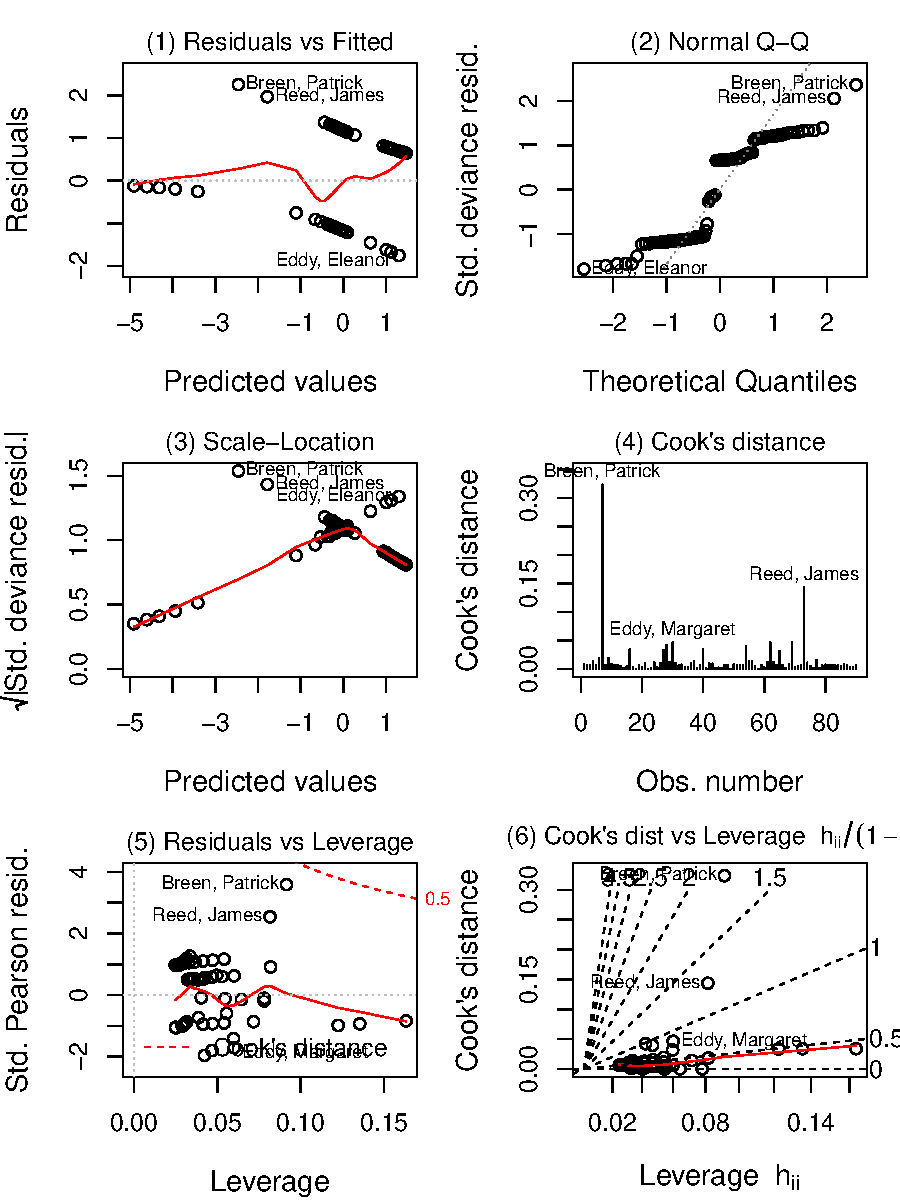
\includegraphics[width=.9\textwidth]{ch07/fig/donner2-plot-1} }

\caption[Diagnostic plots for a glm object, using the fitted model donner.mod3 for the Donner Party data.]{Diagnostic plots for a glm object, using the fitted model \code{donner.mod3} for the Donner Party data. Each plot shows some additional annotations or smoothed curves and labels observations considered noteworthy in terms of influence.\label{fig:donner2-plot}}
\end{figure}


\end{knitrout}
The six plots, corresponding to the values of \code{which}, shown in \figref{fig:donner2-plot} for the \code{donner.mod3} model are:
\begin{enumerate*}
\item a plot of residuals against fitted values.  In a classical linear model, this plot
should appear unstructured (random around the zero line), but for logistic regression
there will always be two sequences of points, corresponding to the 0/1 observations.
\item a normal Q-Q plot of ordered residuals vs.\ the corresponding quantiles of the gaussian distribution. In a classical linear model, all points should follow the dotted reference line,
but this will rarely hold for logistic regression models.
\item a Scale-Location plot of $\sqrt{|\mbox{residuals}|}$ against fitted values,
with a loess smoothed curve showing the trend for variance of the residual to
change with the predicted value.  This is useful to detect non-constant residual
variance in classical models, but in logistic regression, you will almost always
see a U-shaped pattern corresponding to the fact that the variance around the
fitted value is a function of $\sqrt{\hat{p}_i (1-\hat{p}_i)} $.
\item an index plot of Cook's distances versus observation numbers, with the largest \code{id.n} values labeled. 
\item a plot of residuals against leverages, showing contours of Cook's distances.  
Among all of these plots, this is probably the most useful for assessment of
influence in both classical and generalized linear models.  The function
\func{influencePlot} in \pkg{car} provides a better version of this plot,
using the size of a bubble symbol to also show Cook's distance directly.
\item a plot of Cook's distances against leverage/(1-leverage).
In this plot contours of standardized residuals that are equal in magnitude are lines through the origin,
and labeled with their absolute values. Consequently, more influential observations appear toward the top.
\end{enumerate*}
In all these plots, three observations are labeled as noteworthy, by one criterion or another
with a default number given by \code{id.n=3}. Plotting just the residual-leverage graph
(\code{which=5}) with some additional annotations to show the conventional cutoff values
gives \figref{fig:donner2-plot5}.

\begin{knitrout}
\definecolor{shadecolor}{rgb}{1, 0.961, 0.933}\color{fgcolor}\begin{kframe}
\begin{alltt}
\hlstd{op} \hlkwb{<-} \hlkwd{par}\hlstd{(}\hlkwc{mar}\hlstd{=}\hlkwd{c}\hlstd{(}\hlnum{5}\hlstd{,}\hlnum{4}\hlstd{,}\hlnum{4}\hlstd{,}\hlnum{2}\hlstd{)}\hlopt{+}\hlnum{.1}\hlstd{)}
\hlkwd{plot}\hlstd{(donner.mod3,} \hlkwc{which}\hlstd{=}\hlnum{5}\hlstd{,} \hlkwc{cex.id}\hlstd{=}\hlnum{1}\hlstd{,} \hlkwc{cook.levels}\hlstd{=}\hlkwd{c}\hlstd{(}\hlnum{0.25}\hlstd{,} \hlnum{0.5}\hlstd{),} \hlkwc{id.n}\hlstd{=}\hlnum{3}\hlstd{)}
\hlkwd{abline}\hlstd{(}\hlkwc{h}\hlstd{=}\hlkwd{c}\hlstd{(}\hlopt{-}\hlnum{2}\hlstd{,} \hlnum{2}\hlstd{),} \hlkwc{col}\hlstd{=}\hlstr{"gray"}\hlstd{)}
\hlstd{k} \hlkwb{<-} \hlkwd{length}\hlstd{(}\hlkwd{coef}\hlstd{(donner.mod3))}
\hlstd{n} \hlkwb{<-} \hlkwd{nrow}\hlstd{(Donner)}
\hlkwd{abline}\hlstd{(}\hlkwc{v}\hlstd{=}\hlkwd{c}\hlstd{(}\hlnum{2}\hlstd{,} \hlnum{3}\hlstd{)}\hlopt{*}\hlstd{k}\hlopt{/}\hlstd{n,} \hlkwc{col}\hlstd{=}\hlstr{"gray"}\hlstd{)}
\hlkwd{text}\hlstd{(}\hlkwc{x}\hlstd{=}\hlkwd{c}\hlstd{(}\hlnum{2}\hlstd{,} \hlnum{3}\hlstd{)}\hlopt{*}\hlstd{k}\hlopt{/}\hlstd{n,} \hlkwc{y}\hlstd{=}\hlopt{-}\hlnum{2.3}\hlstd{,} \hlkwd{c}\hlstd{(}\hlstr{"2k/n"}\hlstd{,} \hlstr{"3k/n"}\hlstd{))}
\hlkwd{par}\hlstd{(op)}
\end{alltt}
\end{kframe}\begin{figure}[!htbp]


\centerline{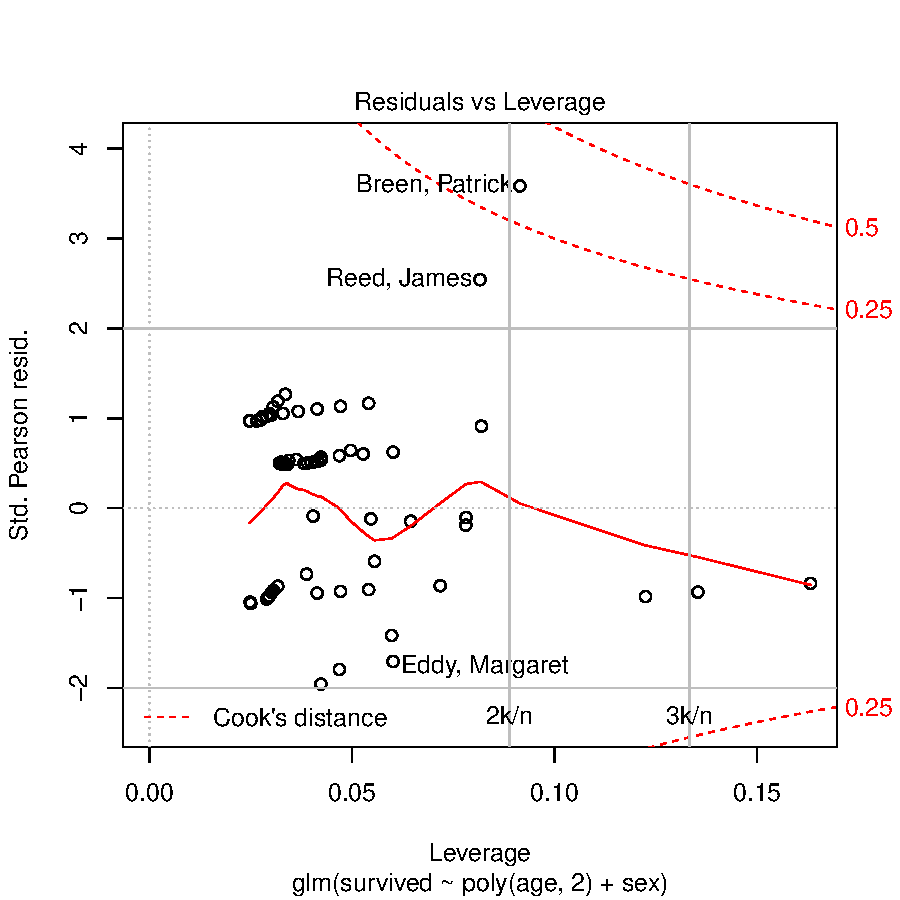
\includegraphics[width=.6\textwidth]{ch07/fig/donner2-plot5-1} }

\caption[Residual vs]{Residual vs. Leverage plot for the Donner data model. Horizontal and vertical reference lines show typical cutoff values for noteworthy residuals and leverage.\label{fig:donner2-plot5}}
\end{figure}


\end{knitrout}

Details of all the diagnostic measures for a given model including the DFBETAs for
individual coefficients can be obtained using \code{influence.measures}.
This can be useful for custom plots not provided elsewhere (see \exref{ex:icu2}).
\begin{knitrout}
\definecolor{shadecolor}{rgb}{1, 0.961, 0.933}\color{fgcolor}\begin{kframe}
\begin{alltt}
\hlstd{infl} \hlkwb{<-} \hlkwd{influence.measures}\hlstd{(donner.mod3)}
\hlkwd{names}\hlstd{(infl)}
\end{alltt}
\begin{verbatim}
## [1] "infmat" "is.inf" "call"
\end{verbatim}
\end{kframe}
\end{knitrout}
The \func{summary} method for the \class{infl} object prints those
observations considered noteworthy on one or more of these statistics, as indicated
by a \code{"*"} next to the value.  
\begin{knitrout}\footnotesize
\definecolor{shadecolor}{rgb}{1, 0.961, 0.933}\color{fgcolor}\begin{kframe}
\begin{alltt}
\hlkwd{summary}\hlstd{(infl)}
\end{alltt}
\begin{verbatim}
## Potentially influential observations of
## 	 glm(formula = survived ~ poly(age, 2) + sex, family = binomial,      data = Donner) :
## 
##                      dfb.1_ dfb.p(,2)1 dfb.p(,2)2 dfb.sxMl dffit   cov.r   cook.d hat    
## Breen, Patrick        0.08   0.65       0.56       0.23     0.69_*  0.93    0.32   0.09  
## Donner, Elizabeth    -0.26  -0.34      -0.22       0.12    -0.40    1.15_*  0.03   0.14_*
## Graves, Elizabeth C. -0.24  -0.37      -0.26       0.10    -0.42    1.20_*  0.03   0.16_*
\end{verbatim}
\end{kframe}
\end{knitrout}


The function \func{influencePlot} in the \Rpackage{car} gives a similar plot, but uses the size (area)
of the plotting symbol to also show the value of Cook's D as shown in \figref{fig:donner2-inflplot}.  
Like other diagnostic plots
in \pkg{car}, it is considerably more general than illustrated here, because
it allows for different \code{id.method}s to label noteworthy points, including
\code{id.method="identify"} for interactive point identification by clicking with
the mouse. The \code{id.n} argument works differently than with \func{plot}, 
because it selects the most extreme \code{id.n} observations on \emph{each} of
the studentized residual, hat value and Cook's D, and labels all of these.

\begin{knitrout}
\definecolor{shadecolor}{rgb}{1, 0.961, 0.933}\color{fgcolor}\begin{kframe}
\begin{alltt}
\hlkwd{library}\hlstd{(car)}
\hlstd{res} \hlkwb{<-} \hlkwd{influencePlot}\hlstd{(donner.mod3,} \hlkwc{id.col}\hlstd{=}\hlstr{"blue"}\hlstd{,} \hlkwc{scale}\hlstd{=}\hlnum{8}\hlstd{,} \hlkwc{id.n}\hlstd{=}\hlnum{2}\hlstd{)}
\hlkwd{text}\hlstd{(}\hlkwc{x}\hlstd{=}\hlkwd{c}\hlstd{(}\hlnum{2}\hlstd{,} \hlnum{3}\hlstd{)}\hlopt{*}\hlstd{k}\hlopt{/}\hlstd{n,} \hlkwc{y}\hlstd{=}\hlopt{-}\hlnum{1.8}\hlstd{,} \hlkwd{c}\hlstd{(}\hlstr{"2k/n"}\hlstd{,} \hlstr{"3k/n"}\hlstd{))}
\end{alltt}
\end{kframe}\begin{figure}[!htbp]


\centerline{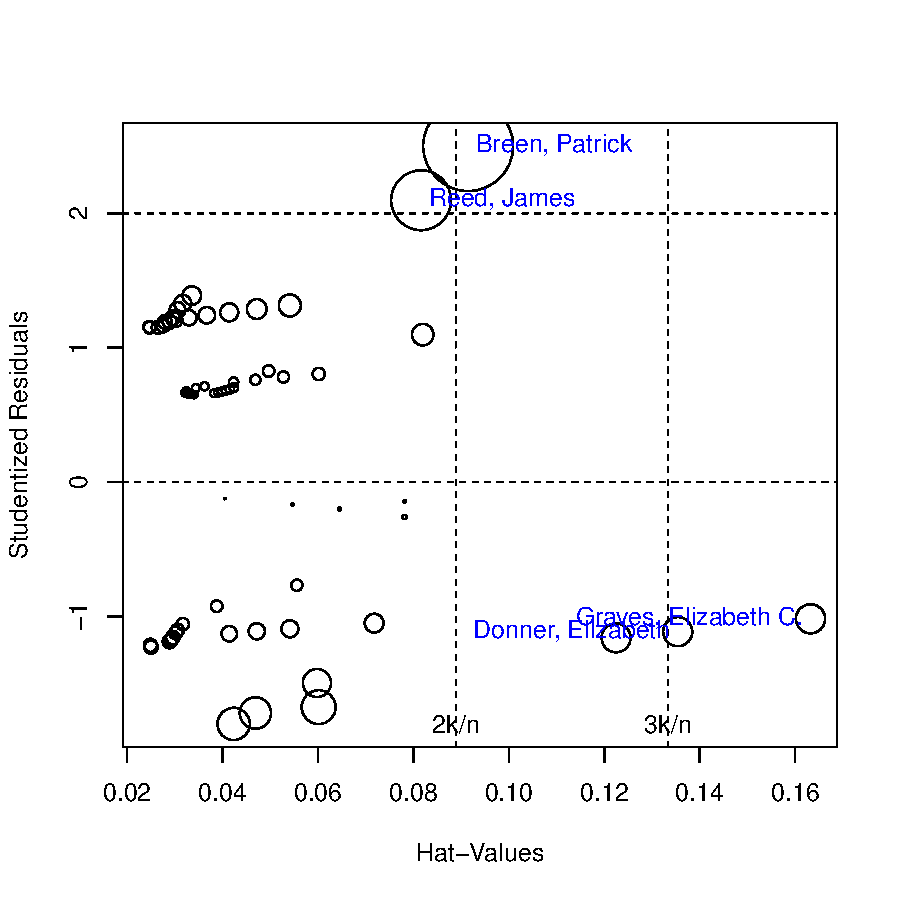
\includegraphics[width=.6\textwidth]{ch07/fig/donner2-inflplot-1} }

\caption[Influence plot (residual vs]{Influence plot (residual vs. leverage) for the Donner data model, showing Cook's D as the size of the bubble symbol. Horizontal and vertical reference lines show typical cutoff values for noteworthy residuals and leverage.\label{fig:donner2-inflplot}}
\end{figure}


\end{knitrout}

Conveniently, \func{influencePlot} returns a data frame containing the influence statistics for the
points identified in the plot (\code{res} in the call above).  We can combine this with the
data values to help learn why these points are considered influential.
\begin{knitrout}
\definecolor{shadecolor}{rgb}{1, 0.961, 0.933}\color{fgcolor}\begin{kframe}
\begin{alltt}
\hlcom{# show data together with diagnostics for influential cases}
\hlstd{idx} \hlkwb{<-} \hlkwd{which}\hlstd{(}\hlkwd{rownames}\hlstd{(Donner)} \hlopt \hlkwd{rownames}\hlstd{(res))}
\hlkwd{cbind}\hlstd{(Donner[idx,}\hlnum{2}\hlopt{:}\hlnum{4}\hlstd{], res)}
\end{alltt}
\begin{verbatim}
##                      age    sex survived StudRes     Hat  CookD
## Breen, Patrick        51   Male      yes   2.501 0.09148 0.5688
## Donner, Elizabeth     45 Female       no  -1.114 0.13541 0.1846
## Graves, Elizabeth C.  47 Female       no  -1.019 0.16322 0.1849
## Reed, James           46   Male      yes   2.098 0.08162 0.3790
\end{verbatim}
\end{kframe}
\end{knitrout}
We can see that Patrick Breen and James Reed%
\footnote{
Breen and Reed, both born in Ireland, were the leaders of their family groups.
Among others, both kept detailed diaries of their experiences, from which most
of the historical record derives.  Reed was also the leader of two relief parties
sent out to find rescue or supplies over the high Sierra mountains, so it is all the
more remarkable that he survived.
}
are unusual because they were
both older men who survived, and have large positive residuals; Breen is the most influential
by Cook's D, but this value is not excessively large. The two women were among the older
women who died.  They are selected here because they have the largest hat values,
meaning they are unusual in terms of the distribution of age and sex, but they are not
particularly influential in terms of Cook's D.

A related graphical display is the collection of index plots provided by
\func{influenceIndexPlot} in \pkg{car}, which plots various influence diagnostics
against the observation numbers in the data.  The \code{id.n} argument here
works to label that number of the most extreme observations \emph{individually} for
each measure plotted.  The following call produces \figref{fig:donner2-indexinfl}.
\begin{knitrout}
\definecolor{shadecolor}{rgb}{1, 0.961, 0.933}\color{fgcolor}\begin{kframe}
\begin{alltt}
\hlkwd{influenceIndexPlot}\hlstd{(donner.mod3,} \hlkwc{vars}\hlstd{=}\hlkwd{c}\hlstd{(}\hlstr{"Cook"}\hlstd{,} \hlstr{"Studentized"}\hlstd{,} \hlstr{"hat"}\hlstd{),}
                   \hlkwc{id.n}\hlstd{=}\hlnum{4}\hlstd{)}
\end{alltt}
\end{kframe}\begin{figure}[!htbp]


\centerline{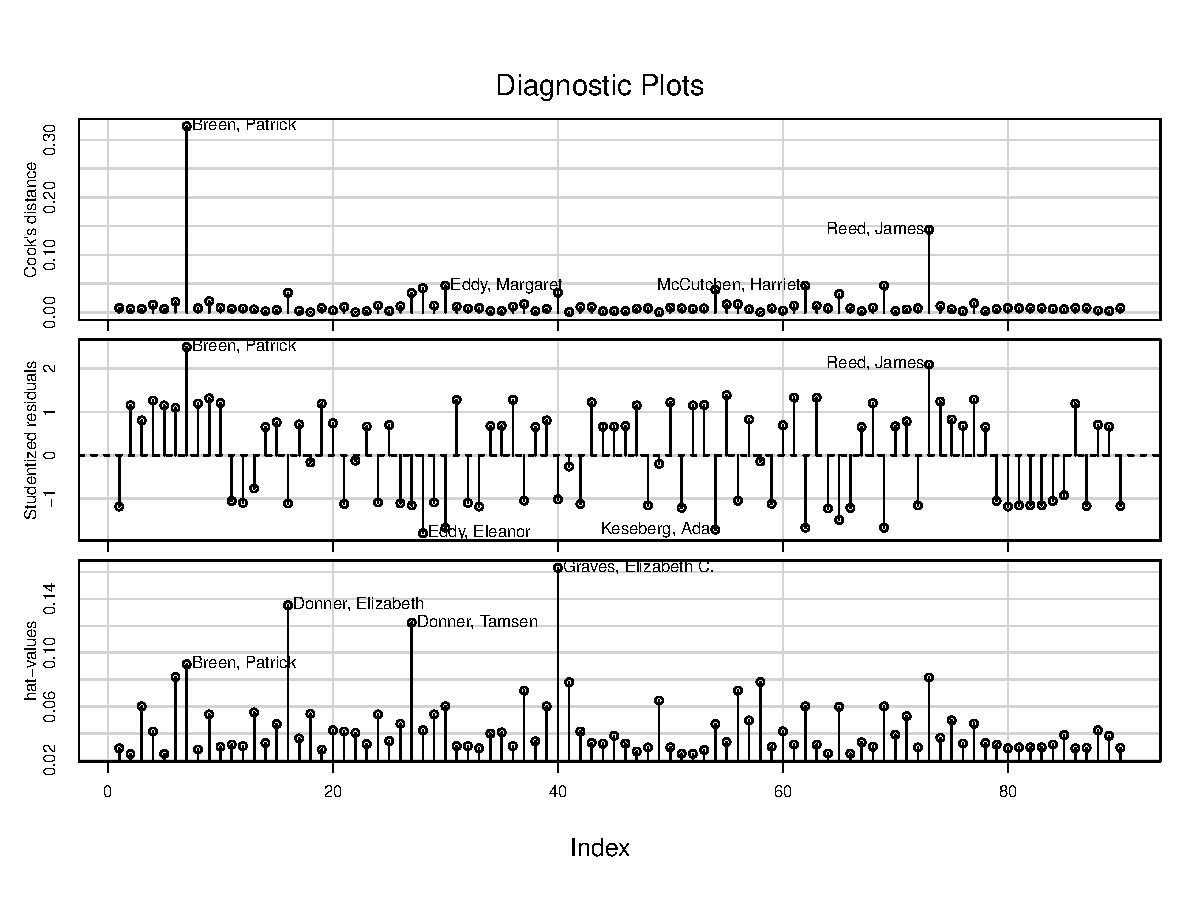
\includegraphics[width=.8\textwidth]{ch07/fig/donner2-indexinfl-1} }

\caption[Index plots of influence measures for the Donner data model]{Index plots of influence measures for the Donner data model. The four most extreme observations on each measure are labeled.\label{fig:donner2-indexinfl}}
\end{figure}


\end{knitrout}
In our opinion, \emph{separate} index plots are often less useful than combined plots such as
the leverage-influence plot that shows residuals, leverage and Cook's D together.
However, the \pkg{car} version in \figref{fig:donner2-indexinfl}
does that too, and allows us to consider how unusual the labeled observations are both individually and in combination.

\end{Example}
% \begin{Example}[icu2]{Death in the ICU}
% \end{Example}

\begin{Example}[icu2]{Death in the ICU}
In \exref{ex:icu1} we examined several models to account for death in the 
\data{ICU} data set. We continue this analysis here, with a focus on
the simple main effects model, \code{icu.glm2}, for which the fitted
logits were shown in \figref{fig:icu1-fit-plot}.
For ease of reference, we restate that model here:
\begin{knitrout}
\definecolor{shadecolor}{rgb}{1, 0.961, 0.933}\color{fgcolor}\begin{kframe}
\begin{alltt}
\hlstd{icu.glm2} \hlkwb{<-} \hlkwd{glm}\hlstd{(died} \hlopt{~} \hlstd{age} \hlopt{+} \hlstd{cancer}  \hlopt{+} \hlstd{admit} \hlopt{+} \hlstd{uncons,}
                \hlkwc{data}\hlstd{=ICU ,} \hlkwc{family}\hlstd{=binomial)}
\end{alltt}
\end{kframe}
\end{knitrout}

The plot of residual vs.\  leverage for this model is shown in \figref{fig:icu2-inflplot}.
\begin{knitrout}
\definecolor{shadecolor}{rgb}{1, 0.961, 0.933}\color{fgcolor}\begin{kframe}
\begin{alltt}
\hlkwd{library}\hlstd{(car)}
\hlstd{res} \hlkwb{<-} \hlkwd{influencePlot}\hlstd{(icu.glm2,} \hlkwc{id.col}\hlstd{=}\hlstr{"red"}\hlstd{,} \hlkwc{scale}\hlstd{=}\hlnum{8}\hlstd{,} \hlkwc{id.cex}\hlstd{=}\hlnum{1.5}\hlstd{,} \hlkwc{id.n}\hlstd{=}\hlnum{3}\hlstd{)}
\end{alltt}
\end{kframe}\begin{figure}[!htbp]


\centerline{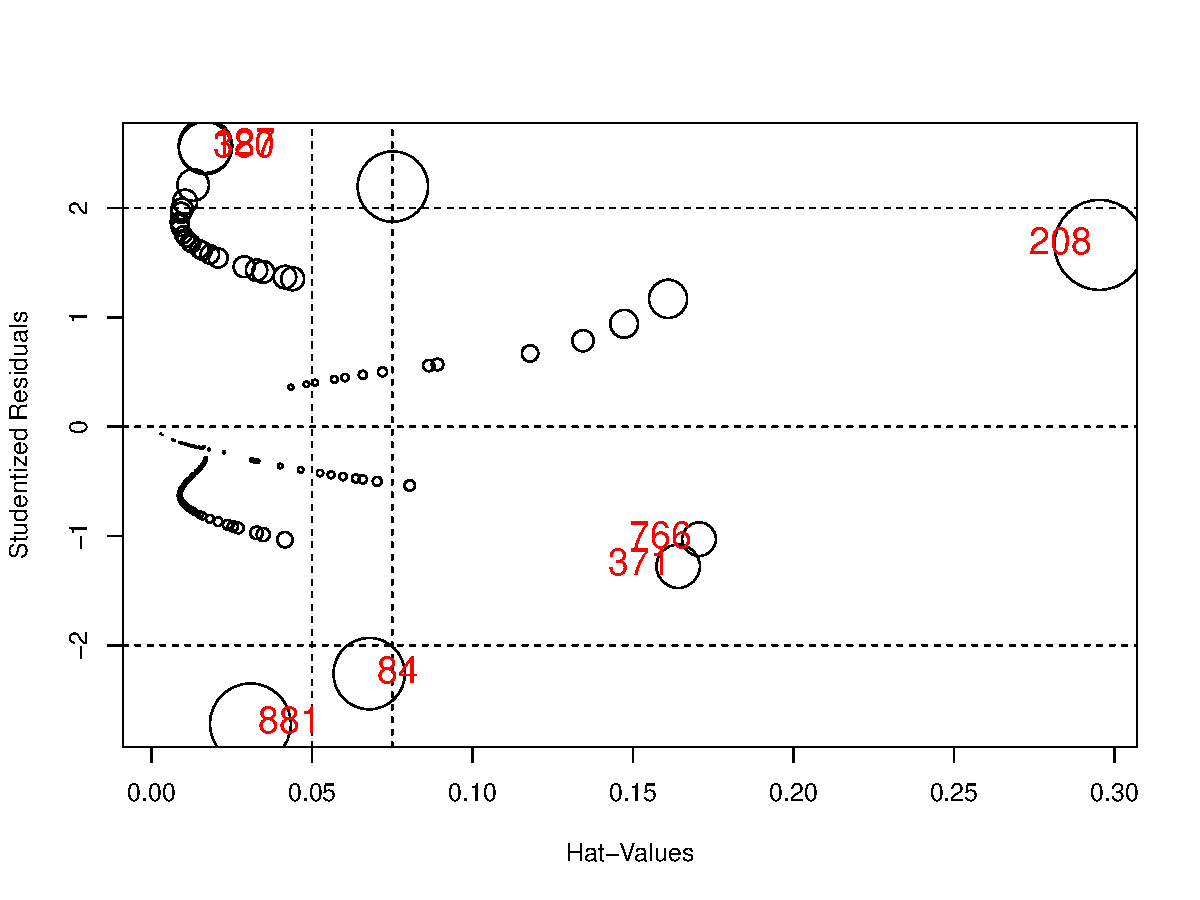
\includegraphics[width=.7\textwidth]{ch07/fig/icu2-inflplot-1} }

\caption[Influence plot for the main effects model for the ICU data]{Influence plot for the main effects model for the ICU data\label{fig:icu2-inflplot}}
\end{figure}


\end{knitrout}

Details for the cases identified in the figure are shown below, again using
\code{rownames(res)} to select the relevant observations from the \data{ICU}
data.

\begin{knitrout}
\definecolor{shadecolor}{rgb}{1, 0.961, 0.933}\color{fgcolor}\begin{kframe}
\begin{alltt}
\hlstd{idx} \hlkwb{<-} \hlkwd{which}\hlstd{(}\hlkwd{rownames}\hlstd{(ICU)} \hlopt \hlkwd{rownames}\hlstd{(res))}
\hlkwd{cbind}\hlstd{(ICU[idx,}\hlkwd{c}\hlstd{(}\hlstr{"died"}\hlstd{,} \hlstr{"age"}\hlstd{,} \hlstr{"cancer"}\hlstd{,} \hlstr{"admit"}\hlstd{,} \hlstr{"uncons"}\hlstd{)], res)}
\end{alltt}
\begin{verbatim}
##     died age cancer     admit uncons StudRes      Hat   CookD
## 84    No  59     No Emergency    Yes -2.2583 0.067807 0.36262
## 371   No  46    Yes Emergency     No -1.2769 0.164082 0.22105
## 766   No  31    Yes Emergency     No -1.0282 0.170619 0.17190
## 881   No  89     No Emergency    Yes -2.7178 0.030806 0.41059
## 127  Yes  19     No Emergency     No  2.5649 0.016792 0.27237
## 208  Yes  70     No  Elective    Yes  1.6618 0.295366 0.45684
## 380  Yes  20     No Emergency     No  2.5481 0.016722 0.26678
\end{verbatim}
\end{kframe}
\end{knitrout}
None of the cases are particularly influential on the model coefficients overall:
the largest Cook's D is only 0.45 for case 208.
This observation also has 
the largest hat value. It is unusual on the predictors
in this sample: a 70 year old man without cancer, admitted on an elective
basis, who nonetheless died. However, this case is also highly unusual 
in having been unconscious on admission for an elective procedure, and
signals that there might have been a coding error or other anomaly
for this observation.

Another noteworthy observation identified here is 
case 881, an 89 year old male, admitted unconscious
as an emergency; this case is poorly predicted because he survived.
Similarly, two other cases (127, 380) with large studentized residuals
are poorly predicted because they died, although they were
young, did not have cancer, and conscious at admission.
However, these cases have relatively small Cook's D values.
From this evidence we might conclude that, case 208 bears further scrutiny,
but none of these cases greatly affects the model, 
its coefficients, or interpretation.

For comparison with \figref{fig:icu2-inflplot}, the related index plot of
these measures is shown in \figref{fig:icu2-infl-index}.

\begin{knitrout}
\definecolor{shadecolor}{rgb}{1, 0.961, 0.933}\color{fgcolor}\begin{kframe}
\begin{alltt}
\hlkwd{influenceIndexPlot}\hlstd{(icu.glm2,} \hlkwc{vars}\hlstd{=}\hlkwd{c}\hlstd{(}\hlstr{"Cook"}\hlstd{,} \hlstr{"Studentized"}\hlstd{,} \hlstr{"hat"}\hlstd{),} \hlkwc{id.n}\hlstd{=}\hlnum{4}\hlstd{)}
\end{alltt}
\end{kframe}\begin{figure}[!htbp]


\centerline{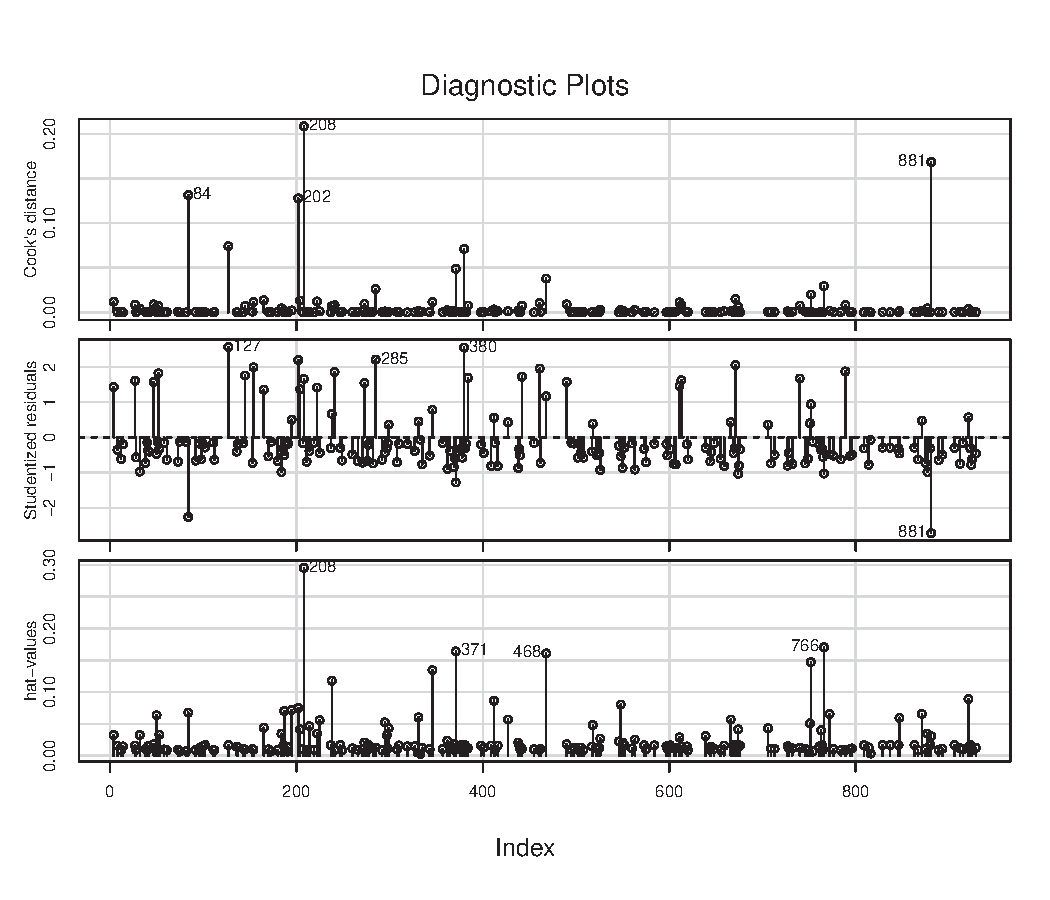
\includegraphics[width=.8\textwidth]{ch07/fig/icu2-infl-index-1} }

\caption[Index plots of influence measures for the ICU data model]{Index plots of influence measures for the ICU data model. The four most extreme observations on each measure are labeled.\label{fig:icu2-infl-index}}
\end{figure}


\end{knitrout}

Cook's D and DFFITS are \emph{overall} measures of the total influence that cases have
on the regression coefficients and fitted values respectively.
It might be that some cases have a large impact on some individual regression coefficients,
but don't appear particularly unusual in these aggregate measures.

One way to study this is to make plots of the DFBETA$_{ij}$ statistics.
Such plots are not available (as far as we know) in \R packages, but it is not hard
to construct them from the result returned by \func{influence.measures}.
To do this, we select the appropriate columns from the \code{infmat} component returned by that
function.
\begin{knitrout}
\definecolor{shadecolor}{rgb}{1, 0.961, 0.933}\color{fgcolor}\begin{kframe}
\begin{alltt}
\hlstd{infl} \hlkwb{<-} \hlkwd{influence.measures}\hlstd{(icu.glm2)}
\hlstd{dfbetas} \hlkwb{<-} \hlkwd{data.frame}\hlstd{(infl}\hlopt{$}\hlstd{infmat[,}\hlnum{2}\hlopt{:}\hlnum{5}\hlstd{])}
\hlkwd{colnames}\hlstd{(dfbetas)} \hlkwb{<-} \hlkwd{c}\hlstd{(}\hlstr{"dfb.age"}\hlstd{,} \hlstr{"dfb.cancer"}\hlstd{,} \hlstr{"dfb.admit"}\hlstd{,} \hlstr{"dfb.uncons"}\hlstd{)}
\hlkwd{head}\hlstd{(dfbetas)}
\end{alltt}
\begin{verbatim}
##       dfb.age dfb.cancer  dfb.admit dfb.uncons
## 8   0.0473397   0.013418  0.0040668  0.0092535
## 12  0.0189876   0.018412 -0.0041744  0.0181058
## 14 -0.0010511   0.014882  0.0262778  0.0055550
## 28  0.0315625   0.018424 -0.0015115  0.0166399
## 32 -0.1640841   0.003788 -0.0365051  0.0234880
## 38 -0.0215252   0.016539 -0.0119366  0.0208033
\end{verbatim}
\end{kframe}
\end{knitrout}

To illustrate this idea, plotting an individual column of \code{dfbetas} using \code{type = "h"}
gives an index plot against the observation number. This is shown in \figref{fig:icu2-dbage}
for the impact on the coefficient for age.
The lines and points are colored
blue or red according to whether the patient lived or died.
Observations for which the $|\mbox{DFBETA}_{\mbox{age}}| > 0.2$ (an arbitrary value)
are labeled.  
\begin{knitrout}
\definecolor{shadecolor}{rgb}{1, 0.961, 0.933}\color{fgcolor}\begin{kframe}
\begin{alltt}
\hlstd{cols}\hlkwb{=}\hlkwd{ifelse} \hlstd{(ICU}\hlopt{$}\hlstd{died}\hlopt{==}\hlstr{"Yes"}\hlstd{,} \hlstr{"red"}\hlstd{,} \hlstr{"blue"}\hlstd{)}
\hlstd{op} \hlkwb{<-} \hlkwd{par}\hlstd{(}\hlkwc{mar}\hlstd{=}\hlkwd{c}\hlstd{(}\hlnum{5}\hlstd{,}\hlnum{5}\hlstd{,}\hlnum{1}\hlstd{,}\hlnum{1}\hlstd{)}\hlopt{+}\hlnum{.1}\hlstd{)}
\hlkwd{plot}\hlstd{(dfbetas[,}\hlnum{1}\hlstd{],} \hlkwc{type} \hlstd{=} \hlstr{"h"}\hlstd{,} \hlkwc{col}\hlstd{=cols,}
     \hlkwc{xlab}\hlstd{=}\hlstr{"Observation index"}\hlstd{,}
     \hlkwc{ylab}\hlstd{=}\hlkwd{expression}\hlstd{(Delta} \hlopt{*} \hlstd{beta[Age]),}
     \hlkwc{cex.lab}\hlstd{=}\hlnum{1.3}\hlstd{)}
\hlkwd{points}\hlstd{(dfbetas[,}\hlnum{1}\hlstd{],} \hlkwc{col}\hlstd{=cols)}
\hlcom{# label some points}
\hlstd{big} \hlkwb{<-} \hlkwd{abs}\hlstd{(dfbetas[,}\hlnum{1}\hlstd{])} \hlopt{>} \hlnum{.25}
\hlstd{idx} \hlkwb{<-} \hlnum{1}\hlopt{:}\hlkwd{nrow}\hlstd{(dfbetas)}
\hlkwd{text}\hlstd{(idx[big], dfbetas[big,}\hlnum{1}\hlstd{],} \hlkwc{label}\hlstd{=}\hlkwd{rownames}\hlstd{(dfbetas)[big],}
     \hlkwc{cex}\hlstd{=}\hlnum{0.9}\hlstd{,} \hlkwc{pos}\hlstd{=}\hlkwd{ifelse}\hlstd{(dfbetas[big,}\hlnum{1}\hlstd{]}\hlopt{>}\hlnum{0}\hlstd{,} \hlnum{3}\hlstd{,} \hlnum{1}\hlstd{),}
     \hlkwc{xpd}\hlstd{=}\hlnum{TRUE}\hlstd{)}
\hlkwd{abline}\hlstd{(}\hlkwc{h}\hlstd{=}\hlkwd{c}\hlstd{(}\hlopt{-}\hlnum{.25}\hlstd{,} \hlnum{0}\hlstd{,} \hlnum{.25}\hlstd{),} \hlkwc{col}\hlstd{=}\hlstr{"gray"}\hlstd{)}
\hlkwd{par}\hlstd{(op)}
\end{alltt}
\end{kframe}\begin{figure}[!htbp]


\centerline{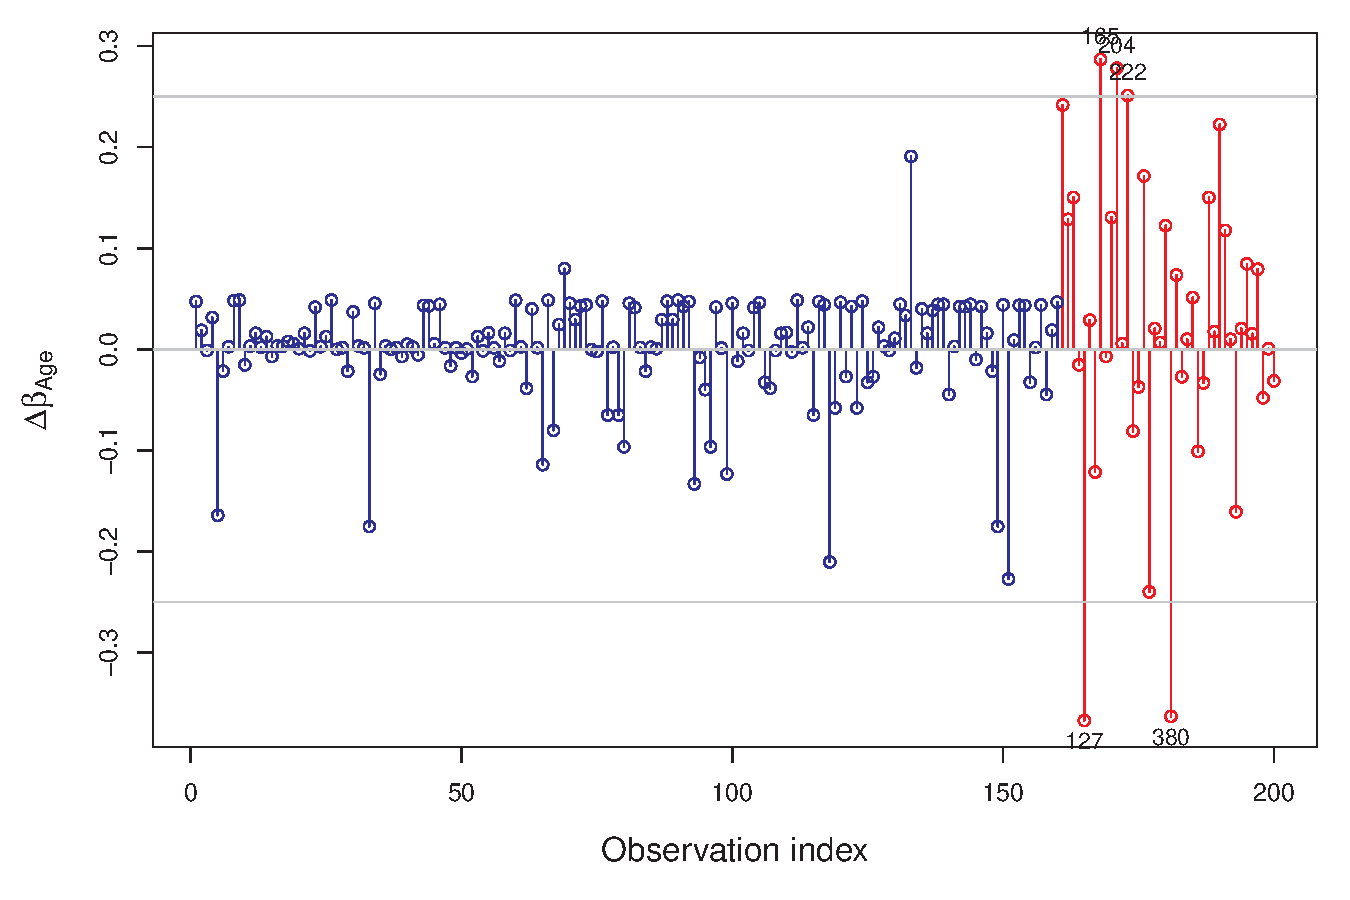
\includegraphics[width=.8\textwidth]{ch07/fig/icu2-dbage-1} }

\caption[Index plot for DFBETA (Age) in the ICU data model]{Index plot for DFBETA (Age) in the ICU data model. The observations are colored blue or red according to whether the patient lived or died.\label{fig:icu2-dbage}}
\end{figure}


\end{knitrout}
None of the labeled points here are a cause for concern, since the standardized DFBETAs
are all relatively small.  However, the plot shows that patients who died have generally
larger impacts on this coefficient.

An alternative to individual index plots is a scatterplot matrix, that shows the pairwise
changes in the regression coefficients for the various predictors.  Here we use
\func{scatterplotMatrix} from \pkg{car} that offers features for additional plot
annotations, including identifying the most unusual points in each pairwise plot.
In each off-diagonal panel, a 95\% data ellipse and linear regression line helps to
show the marginal relationship between the two measures and highlight why the
labeled points are atypical in each plot.%
\footnote{
This plot uses the \code{id.method="mahal"} method
to label the most extreme observations
according to the Mahalanobis distance of each point from the centroid in the plot.
}

\begin{knitrout}
\definecolor{shadecolor}{rgb}{1, 0.961, 0.933}\color{fgcolor}\begin{kframe}
\begin{alltt}
\hlkwd{scatterplotMatrix}\hlstd{(dfbetas,} \hlkwc{smooth}\hlstd{=}\hlnum{FALSE}\hlstd{,} \hlkwc{id.n}\hlstd{=}\hlnum{2}\hlstd{,}
  \hlkwc{ellipse}\hlstd{=}\hlnum{TRUE}\hlstd{,} \hlkwc{levels}\hlstd{=}\hlnum{0.95}\hlstd{,} \hlkwc{robust}\hlstd{=}\hlnum{FALSE}\hlstd{,}
  \hlkwc{diagonal}\hlstd{=}\hlstr{"histogram"}\hlstd{,}
  \hlkwc{groups}\hlstd{=ICU}\hlopt{$}\hlstd{died,} \hlkwc{col}\hlstd{=}\hlkwd{c}\hlstd{(}\hlstr{"blue"}\hlstd{,} \hlstr{"red"}\hlstd{))}
\end{alltt}
\end{kframe}\begin{figure}[!htbp]


\centerline{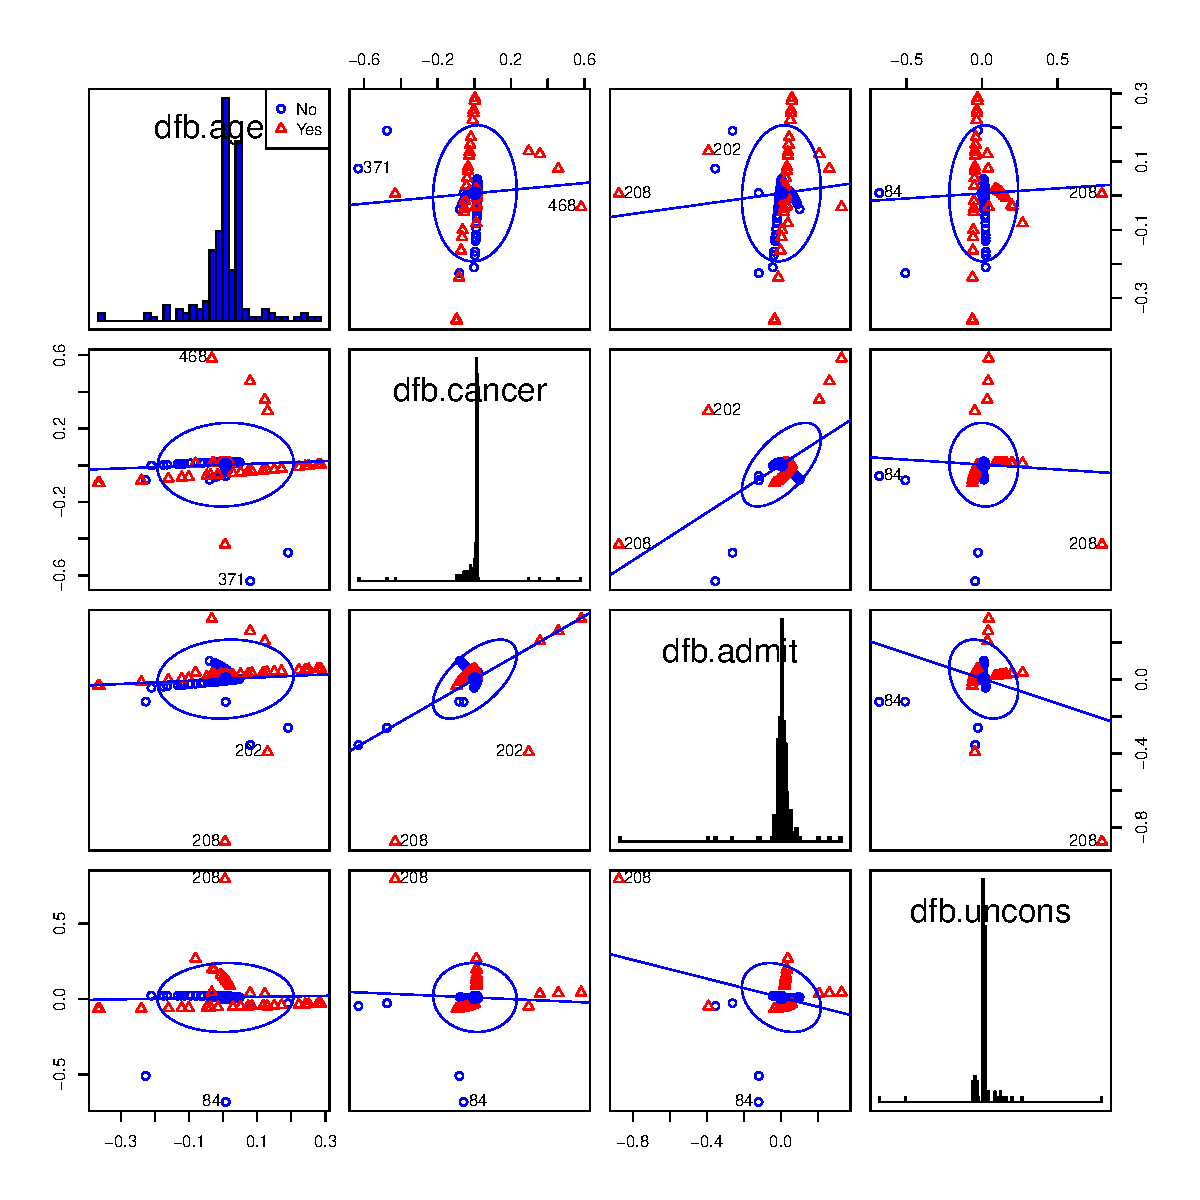
\includegraphics[width=.9\textwidth]{ch07/fig/icu2-dbscatmat-1} }

\caption[Scatterplot matrix for DFBETAs from the model for the ICU data]{Scatterplot matrix for DFBETAs from the model for the ICU data. Those who lived or died are shown with blue circles and red triangles, respectively. The diagonal panels show histograms of each variable.\label{fig:icu2-dbscatmat}}
\end{figure}


\end{knitrout}


\end{Example}

\subsection{Other diagnostic plots}\label{sec:logist-partial}

The graphical methods described in this section are relatively
straight-forward indicators of the adequacy of a particular model,
with a specified set of predictors, each expressed in a given way.
More sophisticated methods have also been proposed, which focus on the need to include a particular predictor and whether its relationship is linear.
These include the \term{component-plus-residual plot}, the
\term{added-variable plot}, and the
\term{constructed variable plot},
which are all analogous to techniques developed in OLS.

\subsubsection{Component-plus-residual plots}\label{sec:component-plus-residual}
The \term{component-plus-residual plot}
(also called a \term{partial residual plot})
proposed originally by 
\citet{LarsenMcCleary:72} is designed to
show whether a given quantitative predictor, $\vec{x}_j$, included linearly in the model,
actually shows a nonlinear relation, requiring transformation.
The essential idea is to move the the linear term for $\vec{x}_j$ back into
the residual, by calculating the \emph{partial residuals},
\begin{equation*}
\vec{r}_j^{\star} = \vec{r} + \beta_j \vec{x}_j
\end{equation*}
Then, a plot of $\vec{r}_j^{\star}$ against $\vec{x}_j$ will have the same slope,
$\beta_j$, as the full model including it among other predictors.
However, any non-linear trend will be shown in the pattern of the points,
usually aided by a smoothed non-parametric curve.

As adapted to logistic regression by \citet{Landwehr-etal:84},
the partial residual for variable $\vec{x}_j$ is defined as
\begin{equation*}%\label{eq:partres}
\vec{r}_j^{\star} = \mat{V}^{-1} \vec{r} + \beta_j \vec{x}_j
% = \frac{\vec{y} - \vec{p}}{ \vec{p} (1 - \vec{p})} \period
\end{equation*}
The partial residual plot is then a plot of $\vec{r}_j^{\star}$ against
$\vec{x}_j$, possibly with the addition of a smoothed lowess curve
\citep{Fowlkes:87} and
a linear regression line to aid interpretation. The linear regression
of the partial residuals on $\vec{x}_j$
has the same slope, $\beta_j$, as in the full model.

If $\vec{x}_j$ affects the binary response linearly, the plot should be approximately linear with a slope approximately equal to $\beta_j$.
A nonlinear plot suggests that $x_j$ needs to be transformed, and
the shape of the relation gives a rough guide to the required
transformation.
For example, a parabolic shape would suggest a term in $\vec{x}_j^2$.
These plots complement the conditional data plots described earlier
(\secref{sec:logist-condplots}), and are most useful when there several quantitative predictors,
so that it is more convenient and sensible to examine their relationships individually.

The \Rpackage{car} implements these plots in the \func{crPlots}
and \func{crPlot} functions. They also work for models with
factor predictors (using parallel boxplots for the factor levels) but not for those with interaction terms.  


\begin{Example}[donner3]{Donner Party}

In \exref{ex:donner2}, we fit several models for the Donner Party
data, and we recall two here to illustrate component-plus-residual
plots.  Both assert additive effects of age and sex, but the model
\code{donner.mod3} allows a quadratic effect of age.

\begin{knitrout}
\definecolor{shadecolor}{rgb}{1, 0.961, 0.933}\color{fgcolor}\begin{kframe}
\begin{alltt}
\hlstd{donner.mod1} \hlkwb{<-} \hlkwd{glm}\hlstd{(survived} \hlopt{~} \hlstd{age} \hlopt{+} \hlstd{sex,} \hlkwc{data}\hlstd{=Donner,} \hlkwc{family}\hlstd{=binomial)}
\hlstd{donner.mod3} \hlkwb{<-} \hlkwd{glm}\hlstd{(survived} \hlopt{~} \hlkwd{poly}\hlstd{(age,}\hlnum{2}\hlstd{)} \hlopt{+} \hlstd{sex,} \hlkwc{data}\hlstd{=Donner,} \hlkwc{family}\hlstd{=binomial)}
\end{alltt}
\end{kframe}
\end{knitrout}
Had we not made exploratory plots earlier (\exref{ex:donner2}), and naively
fit only the linear model in age, \code{donner.mod1}, we could use \func{crPlots} to
check for a non-linear relationship of survival with age as follows, giving \figref{fig:donner-cr1}.

\begin{knitrout}
\definecolor{shadecolor}{rgb}{1, 0.961, 0.933}\color{fgcolor}\begin{kframe}
\begin{alltt}
\hlkwd{crPlots}\hlstd{(donner.mod1,} \hlopt{~}\hlstd{age,} \hlkwc{id.n}\hlstd{=}\hlnum{2}\hlstd{)}
\end{alltt}
\end{kframe}\begin{figure}[!htbp]


\centerline{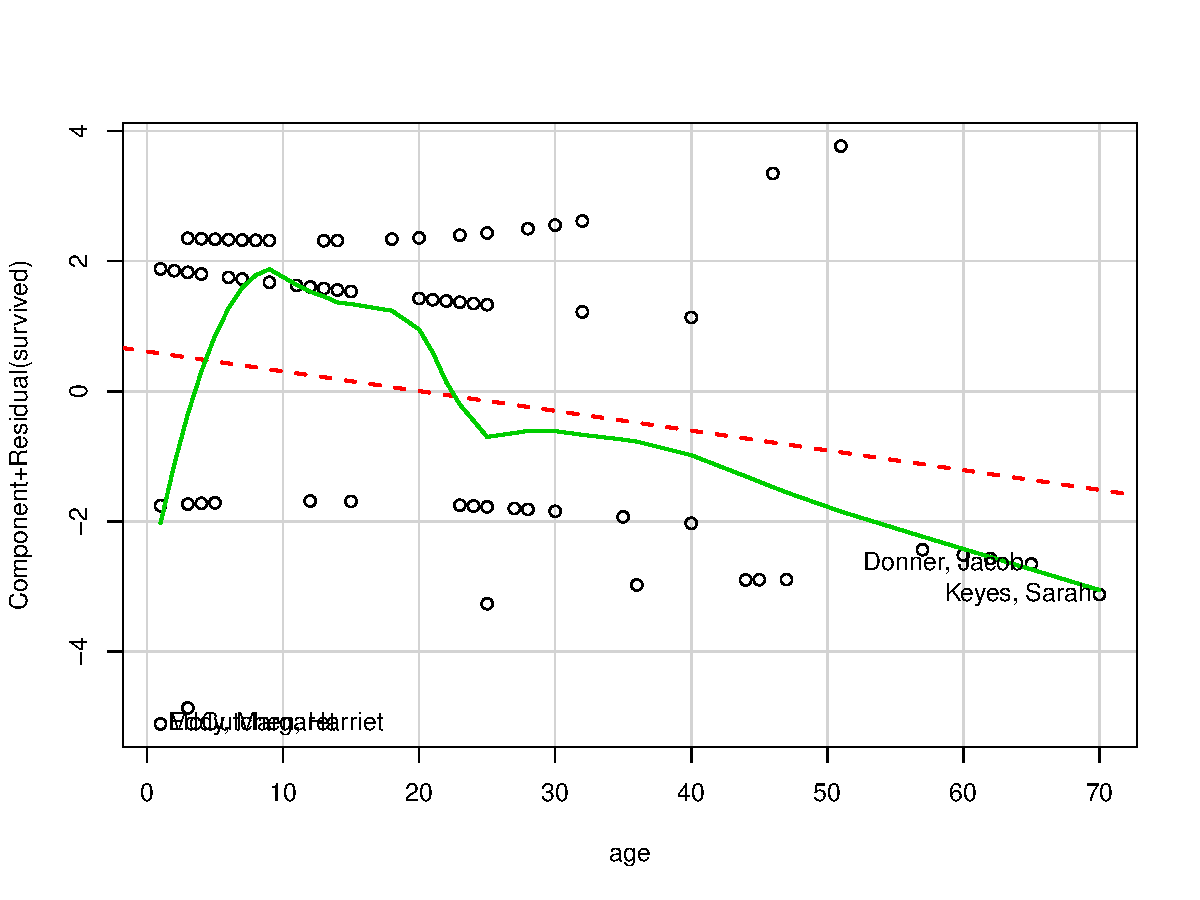
\includegraphics[width=.6\textwidth]{ch07/fig/donner-cr1-1} }

\caption[Component-plus-residual plot for the simple additive linear model]{Component-plus-residual plot for the simple additive linear model, \code{donner.mod1}. The dashed red line shows the slope of age in the full model; the smoothed green curve shows a loess fit with span = 0.5.\label{fig:donner-cr1}}
\end{figure}


\end{knitrout}
The smoothed loess curve in this plot closely resembles the trend we saw in the conditional
plot for age by sex (\figref{fig:donner1-cond3}), suggesting the need to include a non-linear
term for age.  The points identified in this plot, by default, are those with either the most extreme
$x$ values (giving them high leverage) or the largest absolute Pearson residuals
in the full model. The four structured bands of points in the plot correspond to the combinations
of sex and survival.

For comparison, you can see the result of allowing for a non-linear relationship in
age in a partial residual plot for the model \code{donner.mod.3} that includes the
effect \code{poly(age, 2)} for age. Note that the syntax of the \func{crPlots} function 
requires that you specify a \emph{term} in the model, rather than just a predictor variable. 
\begin{knitrout}
\definecolor{shadecolor}{rgb}{1, 0.961, 0.933}\color{fgcolor}\begin{kframe}
\begin{alltt}
\hlkwd{crPlots}\hlstd{(donner.mod3,} \hlopt{~}\hlkwd{poly}\hlstd{(age,}\hlnum{2}\hlstd{),} \hlkwc{id.n}\hlstd{=}\hlnum{2}\hlstd{)}
\end{alltt}
\end{kframe}\begin{figure}[!htbp]


\centerline{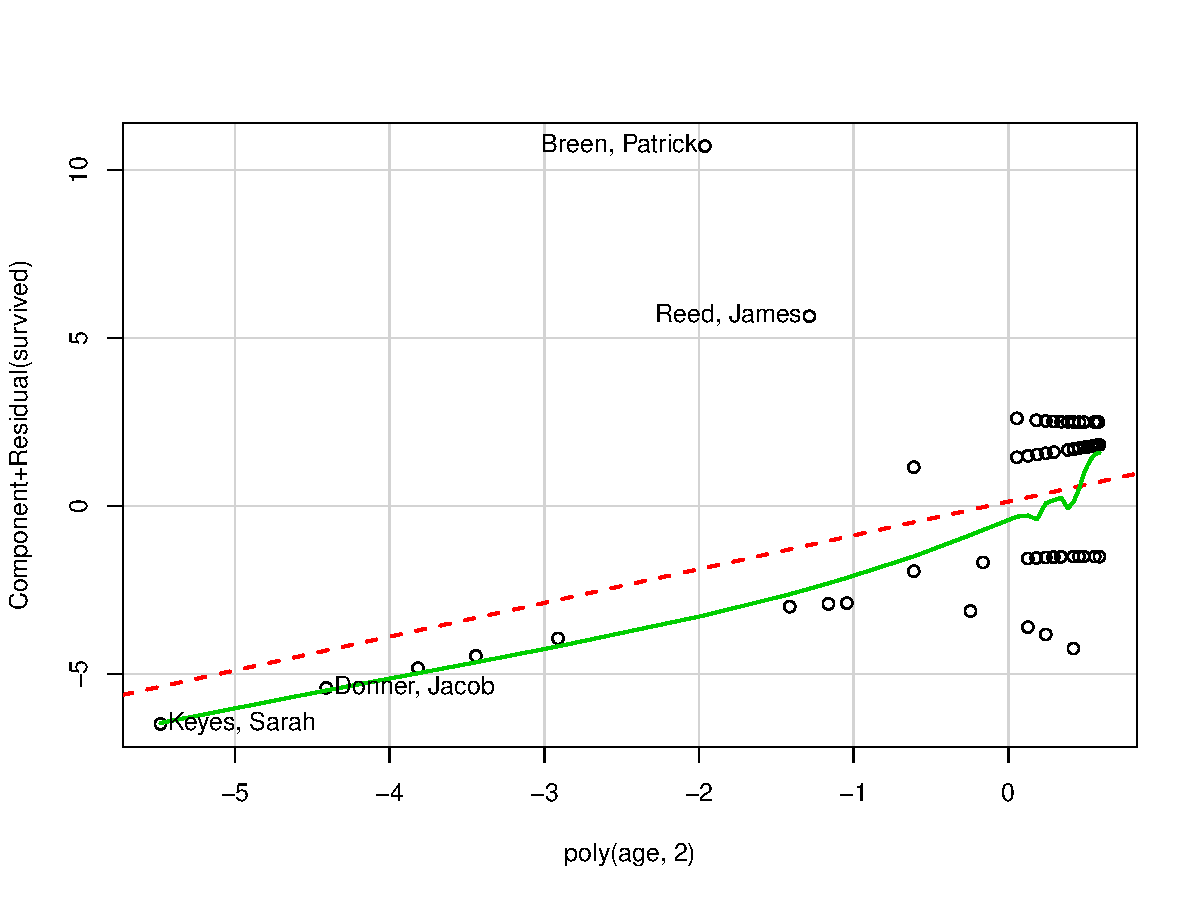
\includegraphics[width=.6\textwidth]{ch07/fig/donner-cr2-1} }

\caption[Component-plus-residual plot for the non-linear additive  model]{Component-plus-residual plot for the non-linear additive  model, \code{donner.mod3}\label{fig:donner-cr2}}
\end{figure}


\end{knitrout}
Except possibly at the extreme right, this plot (\figref{fig:donner-cr2}) shows no indication of a non-linear relationship.

\end{Example}

\subsubsection{Added-variable plots}
Added-variable plots \citep{CookWeisberg:99,WangP:85}
(also called \term{partial-regression plot}s)
are another important tool for diagnosing problems in logistic
regression and other linear or generalized linear models.
These are essentially plots, for each $\vec{x}_i$, of an adjusted 
response, 
$\vec{y}_i^\star = \vec{y} \given \mbox{others}_i$,
against an adjusted predictor, 
$\vec{x}_i^\star = \vec{x}_i \given \mbox{others}_i$,
where $\mbox{others}_i = \mat{X} \notin \vec{x}_i \equiv \mat{X}^{(-i)}$ 
indicates all other predictors excluding $\vec{x}_i$.
As such, they show the \emph{conditional} relationship between the response
and the predictor $\vec{x}_i$, controlling for, or adjusting for, all other
predictors.
Here, $\vec{y}_i^\star$ and $\vec{x}_i^\star$  represent respectively
the residuals from
the regressions of $\vec{y}$ and $\vec{x}_i$ on all the other $x$s
excluding $\vec{x}_i$.

It might seem from this description that each added-variable plot requires
two additional auxiliary logistic regressions to calculate the residuals
$\vec{y}_i^\star$ and $\vec{x}_i^\star$. 
However, \citet{WangP:85}
showed that the added-variable plot may be constructed by following the logistic
regression for the model $\vec{y} \sim \mat{X}^{(-i)}$
with one weighted least squares regression of $\vec{x}_i$ on
$\mat{X}^{(-i)}$ to find the residual part, $\vec{x}_i^{\star}$,  of $\vec{x}$ not predicted
by the other regressors.

Let $\vec{r}$ be the vector of Pearson residuals from the initial logistic
fit of $\vec{y}$ on the variables in $\mat{X}^{(-i)}$,
and let $\mat{H}$ and $\mat{V} = \diag [ \hat{\vec{p}} ( 1 - \hat{\vec{p}})]$
be the hat matrix and $\mat{V}$ matrix from this analysis.
Then, the added-variable plot is a \scat\ of
the residuals $\vec{r}$ against the $\vec{x}_i$-residuals,
\begin{equation*}%\label{eq:addvar}
 \vec{x}_i^{\star} = ( \mat{I} - \mat{H} ) \mat{V}^{1/2} \vec{x} \period
\end{equation*}
% The $\vec{x}_i$-residuals are easily calculated as
% $z_i^{\star} = ( z_i - \hat{z}_i ) \sqrt{v_{ii}}$,
% where $\hat{z}_i$ is the fitted value of $z_i$
% in a weighted least squares regression of $\vec{z}$ on $\mat{X}$
% using the $v_{ii}$ as weights.


There are several important uses of added-variable plots:

First, \emph{marginal} plots of the response variable $\vec{y}$ against the predictor variables
$\vec{x}_i$ can conceal or misrepresent the relationships in a model including several
predictors together due to correlations or associations among the predictors.   This problem is compounded by the fact that graphical methods for discrete responses (boxplots, mosaic plots)
cannot easily show influential observations or non-linear relationships.  Added-variable
plots solve this problem by plotting the residuals,
$\vec{y}_i^\star = \vec{y} \given \mbox{others}_i$, which are less discrete than the
marginal responses in $\vec{y}$.

Second, the numerical measures and graphical methods for detecting influential observations described
earlier in this section are based on the idea of \emph{single-case deletion}, comparing
coefficients or fitted values for the full data, with those that result from deleting each
case in turn.
Yet, it is well-known \citep{Lawrance:1995}, that sets of two (or more) observations can
have \term{joint influence}, that greatly exceeds their individual influential.  
Similarly, the influence of one discrepant point can be offset by another influential point
in an opposite direction, a phenomenon called \term{masking}. The main 
cases of joint influence are illustrated in \figref{fig:joint}.
Added-variable plots, showing the partial regression for one predictor controlling all others
can make such cases visually apparent.

\begin{figure}[!htb]
  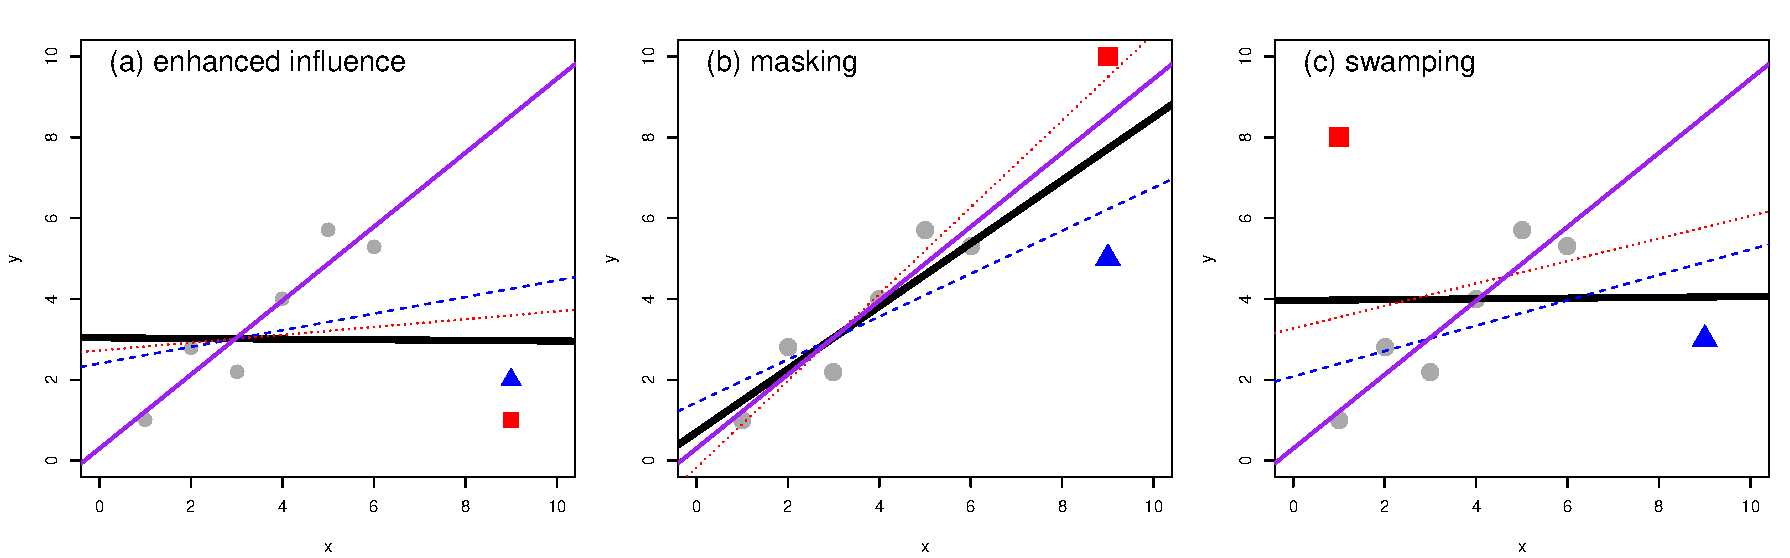
\includegraphics[width=\textwidth]{ch07/fig/joint}
  \caption{Jointly influential points in regression models. In each panel, the thick black line
  shows the regression of $y$ on $x$ using all the data points.  The solid purple line shows
  the regression deleting \emph{both} the red and blue points and the broken and dotted lines
  show the regression retaining only the point in its color in addition to the constant gray points. 
  (a) Two points whose joint influence enhance each other; (b) two points where the influence of one
  is masked by that of the other; (c) two points whose combined influence greatly exceeds the effect of either one individually.}
  \label{fig:joint}
\end{figure}

Finally, given a tentative model using predictors $\vec{x}$, the added-variable plot for
another regressor, $z$ can provide a useful visual assessment of its additional contribution.
An overall test could be based on the difference in $G^2$ for
the enlarged model $\logit(\vec{p}) = \mat{X} \vec{\beta} + \gamma \vec{z}$,
compared to the reduced model
$\logit(\vec{p}) = \mat{X} \vec{\beta}$.
But the added-variable plot shows whether the evidence for including
$z$ is spread throughout the sample or confined to a small subset
of observations.
The regressor $z$ may be a new explanatory variable, or a higher-order term for
variable(s) already in the model.

The \Rpackage{car} implements these plots with the function \func{avPlot}
for a single term and \func{avPlots} for all terms in a linear or generalized
linear model, as shown in the example(s) below.
See \url{http://www.datavis.ca/gallery/animation/duncanAV/} for an animated graphic
showing the transition between a marginal plot of the relationship of $\vec{y}$ to $\vec{x}$
and the added-variable plot of $\vec{y}^\star$ to $\vec{x}^\star$ for the case of 
multiple linear regression with a quantitative response.

\begin{Example}[donner4]{Donner Party}
The simple additive model \code{donner.mod1} for the Donner Party data can be used to illustrate
some features of added-variable plots.  In the call to \func{avPlots} below, we use
color  the plotting symbol to distinguish those who survived vs.\ died,
shape to distinguish men from women.

\begin{knitrout}
\definecolor{shadecolor}{rgb}{1, 0.961, 0.933}\color{fgcolor}\begin{kframe}
\begin{alltt}
\hlstd{col} \hlkwb{<-} \hlkwd{ifelse}\hlstd{(Donner}\hlopt{$}\hlstd{survived}\hlopt{==}\hlstr{"yes"}\hlstd{,} \hlstr{"blue"}\hlstd{,} \hlstr{"red"}\hlstd{)}
\hlstd{pch} \hlkwb{<-} \hlkwd{ifelse}\hlstd{(Donner}\hlopt{$}\hlstd{sex}\hlopt{==}\hlstr{"Male"}\hlstd{,} \hlnum{16}\hlstd{,} \hlnum{17}\hlstd{)}
\hlkwd{avPlots}\hlstd{(donner.mod1,} \hlkwc{id.n}\hlstd{=}\hlnum{2}\hlstd{,} \hlkwc{col}\hlstd{=col,} \hlkwc{pch}\hlstd{=pch,} \hlkwc{col.lines}\hlstd{=}\hlstr{"darkgreen"}\hlstd{)}
\end{alltt}
\end{kframe}
\end{knitrout}

\begin{knitrout}
\definecolor{shadecolor}{rgb}{1, 0.961, 0.933}\color{fgcolor}\begin{figure}[!htbp]


\centerline{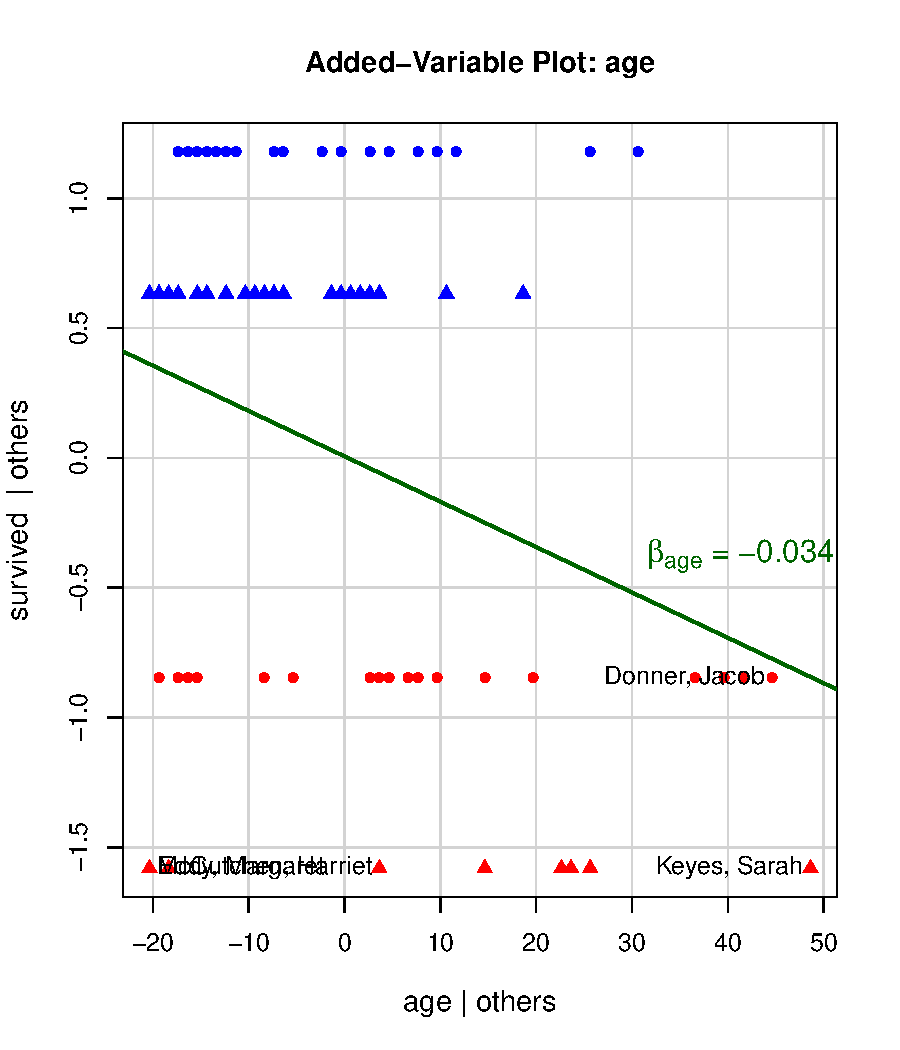
\includegraphics[width=.5\textwidth]{ch07/fig/donner4-avp-1} 
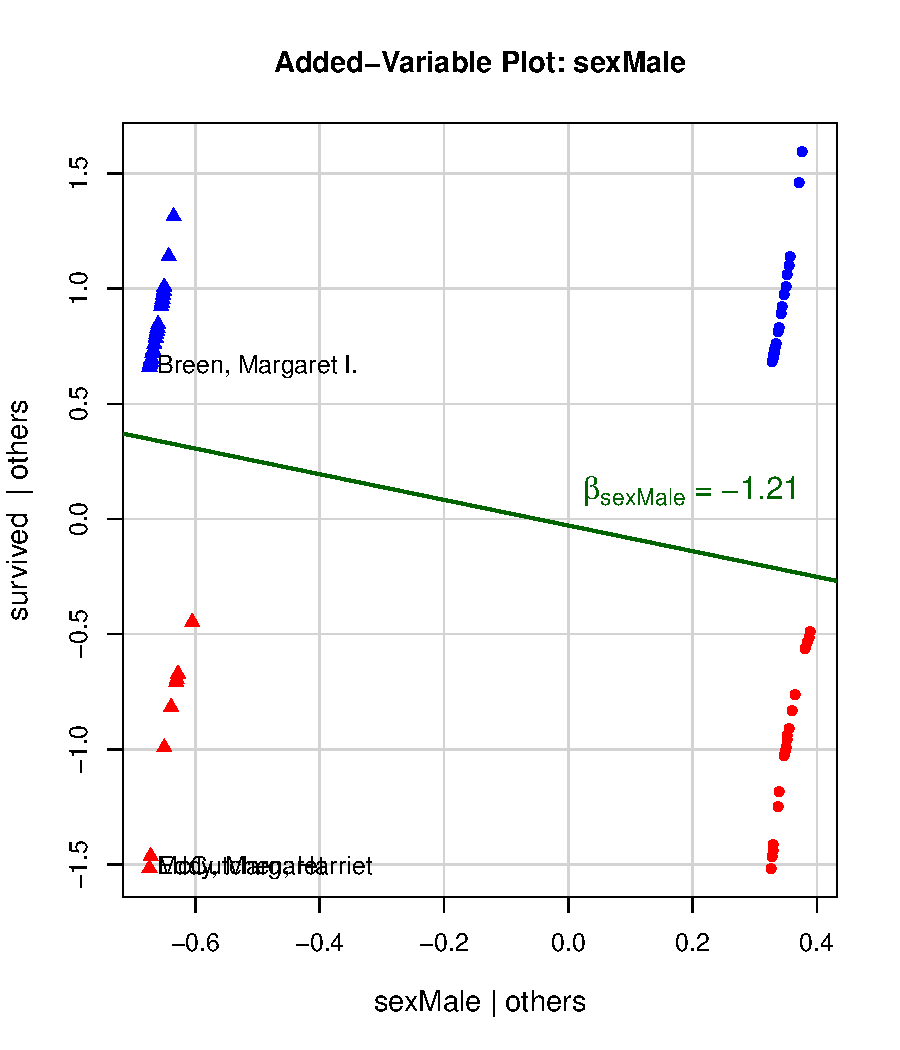
\includegraphics[width=.5\textwidth]{ch07/fig/donner4-avp-2} }

\caption[Added-variable plots for age (left) and sex (right) in the Donner Party main effects model]{Added-variable plots for age (left) and sex (right) in the Donner Party main effects model. Those who survived are shown in blue; those who died in red. Men are plotted with filled circles; women with filled triangles. \label{fig:donner4-avp}}
\end{figure}


\end{knitrout}

These plots have the following properties:
\begin{enumerate}

\item The slope in the simple regression of $\vec{y}_i^\star$ on $\vec{x}_i^\star$
is the same as the partial coefficient $\beta_i$ in the full multiple regression model including
both predictors here (or all predictors in general).

\item The residuals from this regression line are the same as the residuals in the full model.

\item Because the response, \var{survived}, is binary, the vertical axis
$\vec{y}_{\mathrm{age}}^\star$ in the left panel for \var{age} is the part of the logit for
survival that cannot be predicted from \var{sex}.  Similarly, the vertical axis in the
right panel is the part of survival that cannot be predicted from \var{age}.
This property allows the clusters of points corresponding to discrete variables to be
seen more readily, particularly if they are distinguished by visual attributes such
as color and shape, as in \figref{fig:donner4-avp}.

\end{enumerate}


\end{Example}

\begin{Example}[icu3]{Death in the ICU}

We illustrate some of the uses of added-variable plots using the main effects model, 
\code{icu.glm2}, predicting death in the ICU from the variables
\var{age}, \var{cancer}, \var{admit} and \var{uncons}.

To see why marginal plots of the discrete response against each predictor are often
unrevealing for the purpose of model assessment, 
consider the collection of plots in \figref{fig:icu3-marginal}
showing the default plots (spineplots) for the factor response, \var{died}
against each predictor. These show the marginal distribution of each predictor
by the widths of the bars, and highlight the proportion who died by color.
Such plots are useful for some purposes, but not for assessing the adequacy of
the fitted model.

\begin{knitrout}
\definecolor{shadecolor}{rgb}{1, 0.961, 0.933}\color{fgcolor}\begin{kframe}
\begin{alltt}
\hlstd{op} \hlkwb{<-} \hlkwd{par}\hlstd{(}\hlkwc{mfrow}\hlstd{=}\hlkwd{c}\hlstd{(}\hlnum{2}\hlstd{,}\hlnum{2}\hlstd{),} \hlkwc{mar}\hlstd{=}\hlkwd{c}\hlstd{(}\hlnum{4}\hlstd{,}\hlnum{4}\hlstd{,}\hlnum{1}\hlstd{,}\hlnum{2.5}\hlstd{)}\hlopt{+}\hlnum{.1}\hlstd{,} \hlkwc{cex.lab}\hlstd{=}\hlnum{1.4}\hlstd{)}
\hlkwd{plot}\hlstd{(died} \hlopt{~} \hlstd{age,} \hlkwc{data}\hlstd{=ICU,} \hlkwc{col}\hlstd{=}\hlkwd{c}\hlstd{(}\hlstr{"lightblue"}\hlstd{,} \hlstr{"red"}\hlstd{))}
\hlkwd{plot}\hlstd{(died} \hlopt{~} \hlstd{cancer,} \hlkwc{data}\hlstd{=ICU,} \hlkwc{col}\hlstd{=}\hlkwd{c}\hlstd{(}\hlstr{"lightblue"}\hlstd{,} \hlstr{"red"}\hlstd{))}
\hlkwd{plot}\hlstd{(died} \hlopt{~} \hlstd{admit,} \hlkwc{data}\hlstd{=ICU,} \hlkwc{col}\hlstd{=}\hlkwd{c}\hlstd{(}\hlstr{"lightblue"}\hlstd{,} \hlstr{"red"}\hlstd{))}
\hlkwd{plot}\hlstd{(died} \hlopt{~} \hlstd{uncons,} \hlkwc{data}\hlstd{=ICU,} \hlkwc{col}\hlstd{=}\hlkwd{c}\hlstd{(}\hlstr{"lightblue"}\hlstd{,} \hlstr{"red"}\hlstd{))}
\hlkwd{par}\hlstd{(op)}
\end{alltt}
\end{kframe}\begin{figure}[!htbp]


\centerline{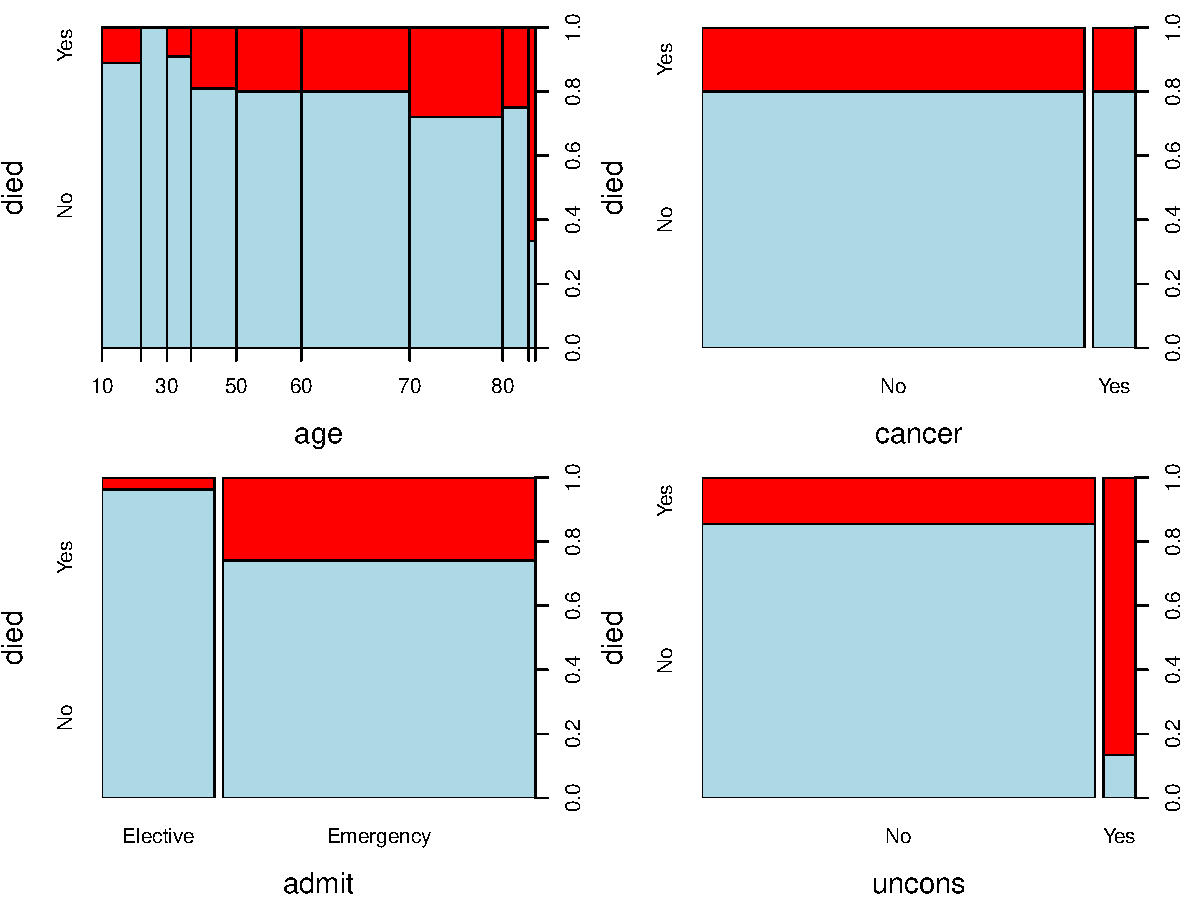
\includegraphics[width=.8\textwidth]{ch07/fig/icu3-marginal-1} }

\caption[Marginal plots of the response died against each of the predictors in the model icu.glm2 for the ICU data]{Marginal plots of the response \code{died} against each of the predictors in the model \code{icu.glm2} for the \data{ICU} data\label{fig:icu3-marginal}}
\end{figure}


\end{knitrout}

% An alternative, pairwise display of the bivariate marginal relations among \emph{all} variables 
% would also show the associations among the predictors in the model.
% \figref{fig:icu3-gpairs} shows a \func{gpairs} display...
% \TODO{Delete this figure and leave it for an exercise.}

% <<icu3-gpairs, h=6, w=6, out.width='.8\\textwidth', cap='All pairwise bivariate plots of the ICU variables'>>=
% library(gpairs)
% gpairs(ICU[,c("died", "age", "cancer", "admit", "uncons")], 
%   diag.pars=list(fontsize=16, hist.color="lightgray"),
%   mosaic.pars=list(gp=shading_Friendly, gp_args=list(interpolate=1:4)))
% @

The added-variable plot for this model is shown in \figref{fig:icu3-avp1}. 
In each plot, the solid red line shows the partial slope, $\beta_j$ for the
focal predictor, controlling for all others.
\begin{knitrout}
\definecolor{shadecolor}{rgb}{1, 0.961, 0.933}\color{fgcolor}\begin{kframe}
\begin{alltt}
\hlstd{pch} \hlkwb{<-} \hlkwd{ifelse}\hlstd{(ICU}\hlopt{$}\hlstd{died}\hlopt{==}\hlstr{"No"}\hlstd{,} \hlnum{1}\hlstd{,} \hlnum{2}\hlstd{)}
\hlkwd{avPlots}\hlstd{(icu.glm2,} \hlkwc{id.n}\hlstd{=}\hlnum{2}\hlstd{,} \hlkwc{pch}\hlstd{=pch,} \hlkwc{cex.lab}\hlstd{=}\hlnum{1.3}\hlstd{)}
\end{alltt}
\end{kframe}\begin{figure}[!htb]


\centerline{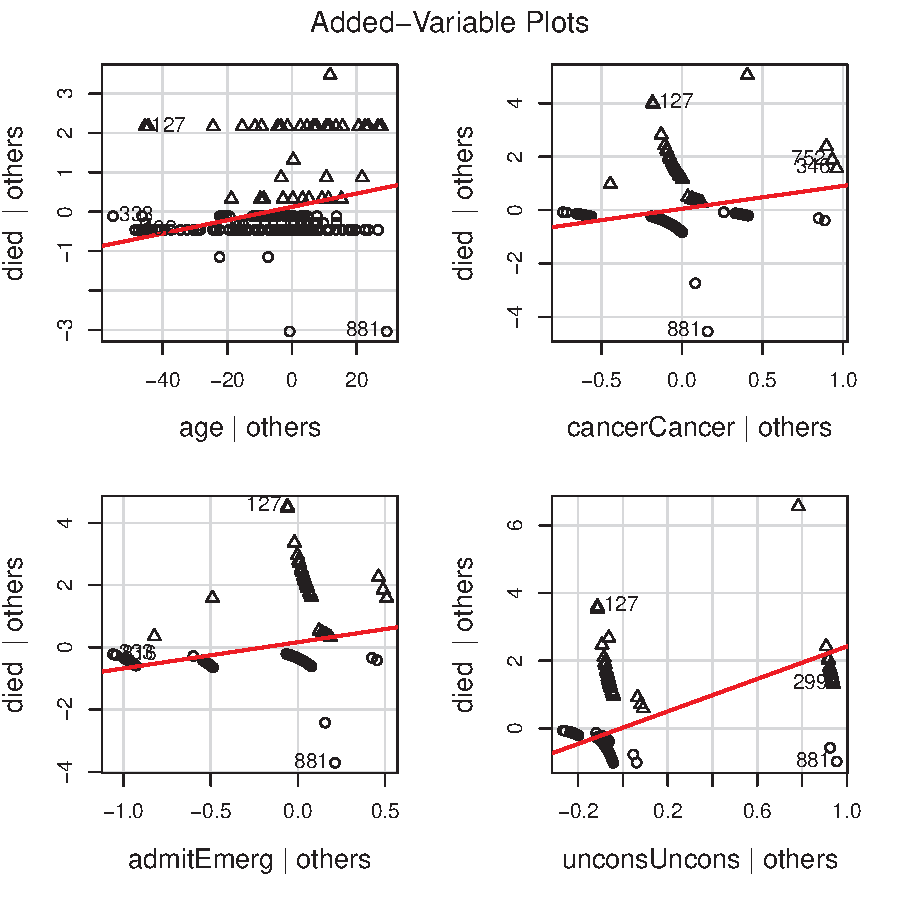
\includegraphics[width=.8\textwidth]{ch07/fig/icu3-avp1-1} }

\caption[Added-variable plots for the predictors in the model for the ICU data.]{Added-variable plots for the predictors in the model for the ICU data. Those who died and survived are shown by triangles ($\triangle$) and circles (\small{$\bigcirc$}) respectively.\label{fig:icu3-avp1}}
\end{figure}


\end{knitrout}
The labeled points in each panel use the default \code{id.method} for
\func{avPlots}, selecting those with either large absolute model residuals or
extreme $\vec{x}_i^\star$ residuals, given all other predictors.
Cases 127 and 881, identified earlier as influential stand out in all these
plots.

Next, we illustrate the use of added-variable plots for checking the 
effect of influential observations on the decision to include 
an additional predictor in some given model.  
In the analysis of the \data{ICU} data using model selection methods,
the variable \var{systolic} (systolic blood pressure at admission)
was nominated by several different procedures.  Here we take a closer look
at the evidence for inclusion of this variable in a predictive model.
We fit a new model adding \var{systolic} to the others and test
the improvement with a likelihood ratio test:
\begin{knitrout}
\definecolor{shadecolor}{rgb}{1, 0.961, 0.933}\color{fgcolor}\begin{kframe}
\begin{alltt}
\hlstd{icu.glm2a} \hlkwb{<-} \hlkwd{glm}\hlstd{(died} \hlopt{~} \hlstd{age} \hlopt{+} \hlstd{cancer}  \hlopt{+} \hlstd{admit} \hlopt{+} \hlstd{uncons} \hlopt{+} \hlstd{systolic,}
                 \hlkwc{data}\hlstd{=ICU,} \hlkwc{family}\hlstd{=binomial)}
\hlkwd{anova}\hlstd{(icu.glm2, icu.glm2a,} \hlkwc{test}\hlstd{=}\hlstr{"Chisq"}\hlstd{)}
\end{alltt}
\begin{verbatim}
## Analysis of Deviance Table
## 
## Model 1: died ~ age + cancer + admit + uncons
## Model 2: died ~ age + cancer + admit + uncons + systolic
##   Resid. Df Resid. Dev Df Deviance Pr(>Chi)  
## 1       195        139                       
## 2       194        136  1     3.52    0.061 .
## ---
## Signif. codes:  0 '***' 0.001 '**' 0.01 '*' 0.05 '.' 0.1 ' ' 1
\end{verbatim}
\end{kframe}
\end{knitrout}
So, the addition of systolic blood pressure is nearly significant at the conventional $\alpha=0.05$
level.  The added-variable plot for this variable in \figref{fig:icu3-avp2}
shows the strength of evidence for its contribution, above and beyond the other variables
in the model, as well as the partial leverage and influence of individual points.
\begin{knitrout}
\definecolor{shadecolor}{rgb}{1, 0.961, 0.933}\color{fgcolor}\begin{kframe}
\begin{alltt}
\hlkwd{avPlot}\hlstd{(icu.glm2a,} \hlstr{"systolic"}\hlstd{,} \hlkwc{id.n}\hlstd{=}\hlnum{3}\hlstd{,} \hlkwc{pch}\hlstd{=pch)}
\end{alltt}
\end{kframe}\begin{figure}[!htbp]


\centerline{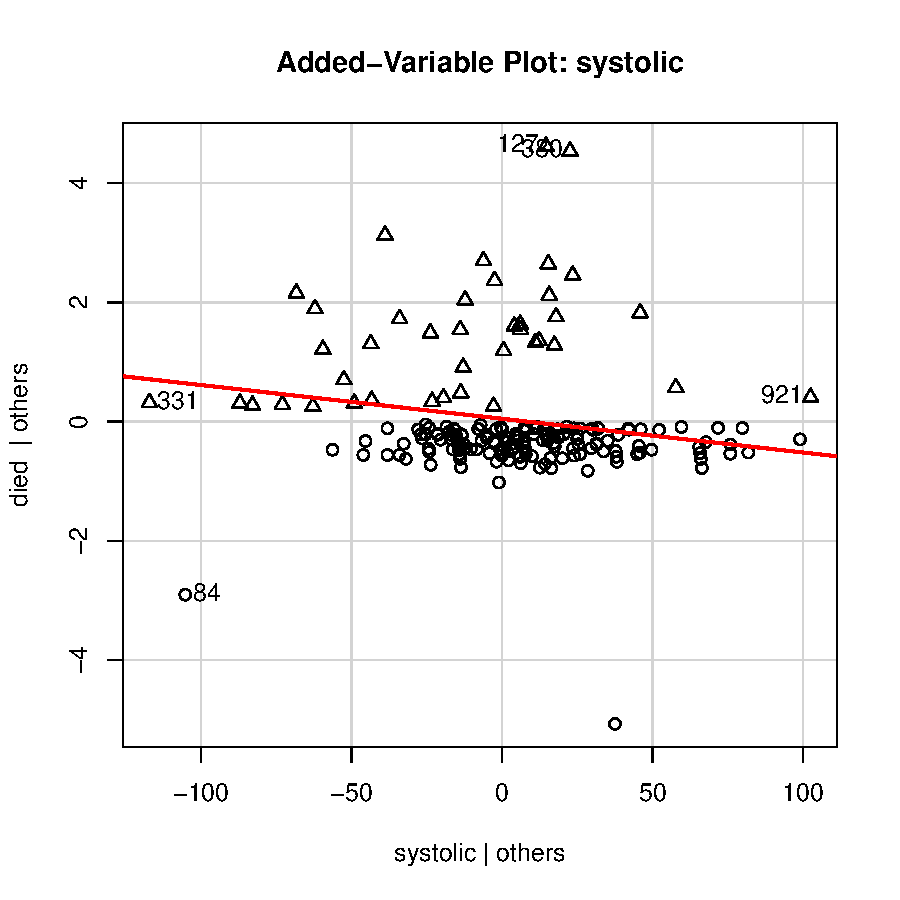
\includegraphics[width=.6\textwidth]{ch07/fig/icu3-avp2-1} }

\caption[added-variable plot for the effect of adding systolic blood pressure to the main effects model for the ICU data]{added-variable plot for the effect of adding systolic blood pressure to the main effects model for the ICU data.\label{fig:icu3-avp2}}
\end{figure}


\end{knitrout}
In this plot, cases 331 and 921 have high partial leverage, but they are not influential.
Case 84, however, has high leverage and a large residual, so is possibly influential on the
evidence for inclusion of \var{systolic} in the model.
Note also that the partial regression line in this plot nicely separates nearly all the patients who died
from those who survived.

\end{Example}

\section{Polytomous response models}\label{sec:logist-poly}

Polytomous response data arise when the outcome variable, $Y$,
takes on $m > 2$ discrete values.  For example, 
\begin{seriate}
 \item patients may record that their improvement after treatment is ``none,''
``some'' or ``marked;''
 \item high school students may choose a general, vocational or
academic program;
 \item women's labor force participation may be recorded in a survey
 as not working outside the home, working part-time, or working full-time;
 \item Canadian voters may express a preference for
the Conservative, Liberal, NDP, Green party.
\end{seriate}
These response categories may be considered ordered or simply
nominal.

In this situation, there are several different
ways to model the response probabilities.  Let \(\pi_{ij} \equiv
\pi_j \,  ( \vec{x}_i )\) be the probability of response $j$ for case
or group $i$, given the predictors $\vec{x}_i$.
Because \(\sum_j \,  \pi_{ij} = 1\), only \(m - 1\) of
these probabilities are independent.  The essential idea here is to
construct a model for the polytomous (or multinomial)
response composed of $m-1$
logit comparisons among the response categories in a similar way
to how factors are treated in the predictor variables.

The simplest approach uses
the 
\term{proportional odds model}, described in \secref{sec:ordinal}.
This model applies only when the response is ordinal
(as in improvement after therapy)
\emph{and} an additional assumption
(the proportional odds assumption) holds. 
This model can be be fit using \func{polr} in the \Rpackage{MASS},
\func{lrm} in the \Rpackage{rms}, and \func{vglm} in \pkg{VGAM}.

However, if the
response is purely nominal (e.g., vote Conservative, Liberal, NDP, Green),
or if the proportional odds assumption is untenable, another particularly
simple strategy is to fit separate models to a set of \(m - 1\)
\term{nested dichotomies} derived from the polytomous response
(described in \secref{sec:nested}). 
This method allows you to resolve the differences
among the $m$ response categories into independent statistical questions
(similar to orthogonal contrasts in ANOVA).
For example, for women's labor force participation, it might be 
substantively interesting to contrast not working vs.\  (part-time and full-time)
and then part-time vs.\ full-time for women who are working.
You fit such nested
dichotomies by running the $m-1$ binary logit models and combining the
statistical results.

The most general approach is the \term{generalized logit model},
also called the \term{multinomial logit model}. 
This model fits \emph{simultaneously} the $m-1$ simple logit models against
a baseline or reference category, for example, the last category, $m$.
With a 3-category response, there are two generalized logits,
$L_{i1} = \log({\pi_{i1}/\pi_{i3}})$ and
$L_{i2} = \log({\pi_{i2}/\pi_{i3}})$, contrasting response categories 1 and
2 against category 3.
In this approach, it doesn't matter which response category is chosen
as the baseline, because all pairwise comparisons can be recovered
from whatever is estimated.  This model is conveniently fitted using
\func{multinom} in \pkg{nnet}.

\subsection[Ordinal response]{Ordinal Response: Proportional Odds Model}%
\label{sec:ordinal}

%\subsection[Ordinal response]{Ordinal Response: Proportional Odds Model}%
%\label{sec:ordinal}
\ixon{proportional odds model}

For an ordered response $Y$, with categories $j = 1, 2, \dots m$, the ordinal nature
of the response can be taken into account by forming logits based on 
the $m-1$ adjacent category cutpoints between successive categories.
That is, if the cumulative probabilities are
\begin{equation*}
\Pr (Y \le j \given \vec{x}) = \pi_1 (\vec{x}) + \pi_2 (\vec{x}) + \cdots \pi_j (\vec{x}) \comma
\end{equation*}
then the \term{cumulative logit} for category $j$ is  defined as
\begin{equation}\label{eq:cumlogit}
L_j \equiv \logit [\Pr (Y \le j \given \vec{x})] =
\log \frac {\Pr (Y \le j \given \vec{x})}{\Pr (Y > j \given \vec{x})} = 
\log \frac {\Pr (Y \le j \given \vec{x})}{1 - \Pr (Y \le j \given \vec{x})} 
\end{equation}
for $j = 1, 2, \dots m-1$.

In our running example of responses to arthritis treatment, the actual
response variable is \var{Improved}, with ordered levels
\code{"None" < "Some" < "Marked"}.  In this case, the cumulative logits
would be defined as
\begin{equation*}
  L_1
 = \log  \frac{ \pi_{1} (\vec{x}) } { \pi_{2} (\vec{x}) +  \pi_{3} (\vec{x})}
 = \mbox{logit ( None vs. [Some or Marked] )}
  \]
  \[
  L_2
 = \log  \frac{  \pi_{1} (\vec{x})   +  \pi_{2} (\vec{x})  } { \pi_{3} (\vec{x}) }
 = \mbox{logit ( [None or Some] vs. Marked)} \comma
\end{equation*}
where $\vec{x}$ represents the predictors (sex, treatment and age).

The \term{proportional odds model} (PO) \citep{Mccullagh:1980} proposes a simple
and parsimonious account of these effects, where the predictors in $\vec(x)$
are constrained to have the same slopes for all cumulative logits,

\begin{equation}\label{eq:propodds}
  L_j = \alpha_j + \vec{x}\trans \vec{\beta} \quad\quad j=1, \dots , m-1 \period
\end{equation}
That is, the effect of the predictor $x_i$ is the same, $\beta_i$, for all
cumulative logits. The cumulative logits differ only in their intercepts.
In this formulation, the $\{ \alpha_j \}$ increase with $j$, because
$\Pr (Y \le j \given \vec{x})$ increases with $j$ for fixed $\vec{x}$.%
\footnote{
Some authors and some software describe the PO model in terms of
$\logit [\Pr (Y > j \given \vec{x})]$, so the signs and order of the
intercepts, $\alpha_j$ are reversed.
}
\figref{fig:podds} portrays the PO model for a single quantitative predictor
$x$ with $m=4$ response categories.  

\begin{figure}
 \centering
 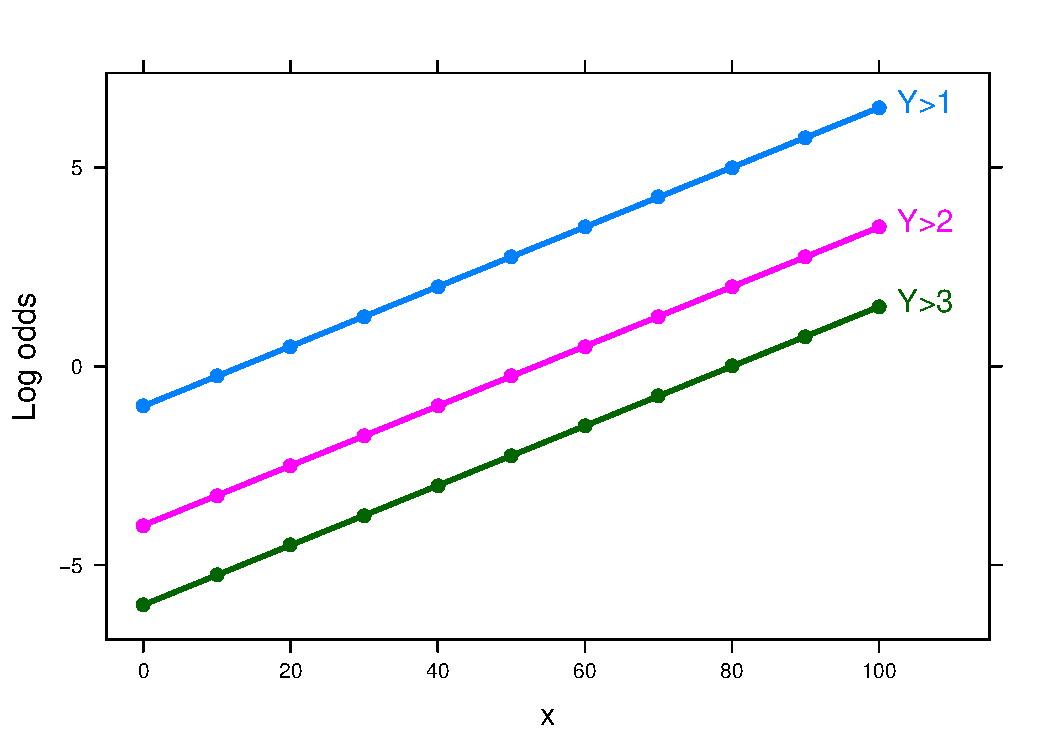
\includegraphics[width=.49\textwidth]{ch07/fig/podds2}
 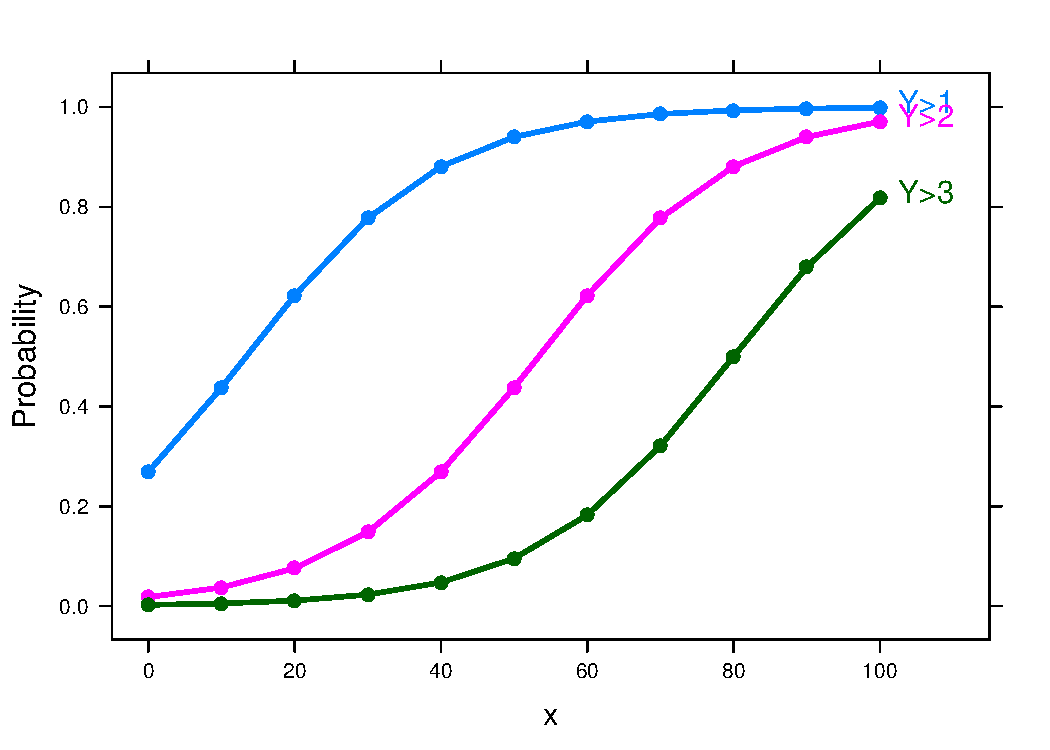
\includegraphics[width=.49\textwidth]{ch07/fig/podds1}
 \caption{Proportional odds model for an ordinal response.  The model assumes equal slopes for the cumulative response logits. Left: logit scale; right: probability scale.}
 \label{fig:podds}
\end{figure}

The name ``proportional odds'' stems from the fact that under \eqref{eq:propodds},
for fixed $\vec{x}$, the cumulative log odds (logits) for categories $j$ and $j\prime$
are constant, $(\alpha_j - \alpha_{j\prime})$, so the odds, $\exp (\alpha_j - \alpha_{j\prime})$
have a constant ratio, or are propoprtional.
Similarly, 
the ratio of the cumulative odds of making a response $Y \le j$ at values of the
predictors $\vec{x} = \vec{x}_1$ are $\exp( (\vec{x}_1 - \vec{x}_2)\trans \vec{\beta} )$
times the odds of this response at $\vec{x} = \vec{x}_2$, so the log cumulative odds
ratio is proportional to the difference between $\vec{x}_1$ and $\vec{x}_2$.

\subsubsection{Latent variable interpretation}
For a binary response, an alternative motivation for logistic regression
regards the relation of the observed $Y$ as arising from a continuous, unobserved,
(latent) response variable, $\xi$ representing the propensity for a
``success'' (1) rather than ``failure'' (0).  
The latent response is assumed to be linearly related to the predictors $\vec{x}$
according to 
\begin{equation}\label{eq:latent}
 \xi_i = \alpha + \vec{x}_i \trans \beta + \epsilon_i 
        = \alpha + \beta_1 x_{i1} + \cdots + \beta_p x_{ip} + \epsilon_i
\end{equation}
However, we can only observe $Y_i =1$ when $\xi_i$ passes some threshold,
that with some convenient scaling can be taken as
$\xi_i > 0 \implies Y_i=1$.%
\footnote{
The latent variable derivation of logistic regression (and the related probit model)
was fundamental in the history of statistical methods for discrete response outcomes.
\TODO{Fill in historical references: psychophysics, toxicology, political science, ...}
}

The latent variable motivation extends directly to an ordinal response under the PO model. 
We now assume that there is a set of $m-1$ thresholds,
$\alpha_1 < \alpha_2 < \cdots < \alpha_{m-1}$ for the latent variable
$\xi_i$ in \eqref{eq:latent} and we observe
\begin{equation*}
  Y_i = j \quad \mbox{if} \quad \alpha_{j-1} < \xi_i \le \alpha_j \comma
\end{equation*}
with appropriate modifications to the inequalities at the end points.  

%\TODO{Add a schematic graph here: Fig 14.10 from Fox:2008, which he adapted from Agresti:1990, Fig 9.2}

\begin{figure}
 \centering
 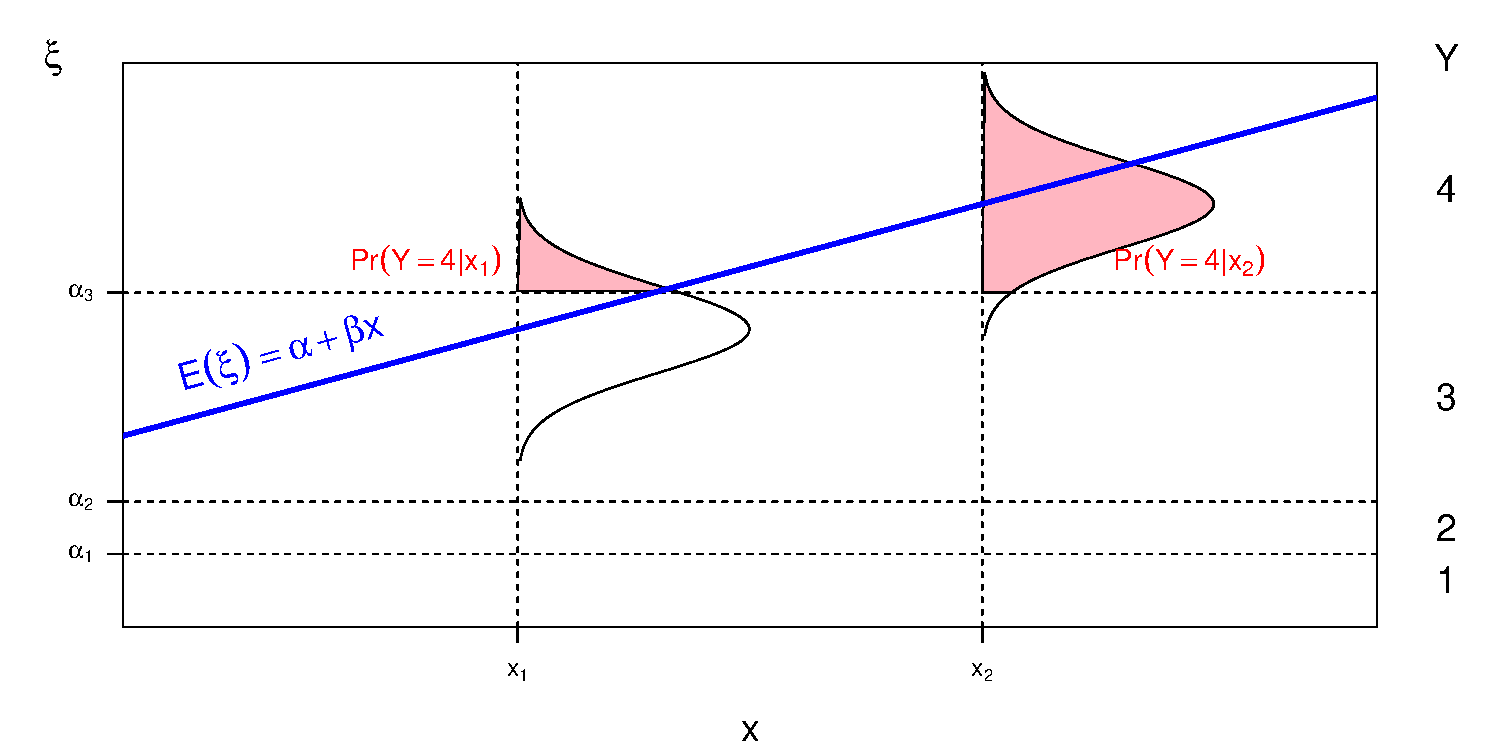
\includegraphics[width=.9\textwidth]{ch07/fig/latent}
 \caption{Latent variable representation of the proportional odds model for $m=4$ response categories and a single quantitative predictor, $x$.
 \emph{Source}: Adapted from \citet[Fig 14.10]{Fox:2008}, using code provided by John Fox.}
 \label{fig:latent}
\end{figure}

This is illustrated in \figref{fig:latent} for a response with $m=4$ 
ordered categories and a single quantitative predictor, $x$.  The observable
response $Y$ categories are shown on the right vertical axis, and the
corresponding latent continuous variable $\xi$ on the left axis
together with the thresholds $\alpha_1, \alpha_2, \alpha_3$.
The (conditional) logistic distribution of $\xi$ is shown at two values  
of $x$, and the shaded areas under the curve give the conditional probabilities
$\Pr (Y=4 \given x_i)$ for the two values $x_1$ and $x_2$.


\subsubsection{Fitting the proportional odds model}

As mentioned earlier, there are a number of different \R packages that
provide facilities for fitting the PO model. These have somewhat different
capabilities for reporting results, testing hypotheses and plotting,
so we generally use \func{polr} in the \Rpackage{MASS}, except where
other packages offer greater convenience.

Unless the response variable has numeric values, it is important to ensure
that it has been defined as an \emph{ordered} factor (using \func{ordered}).
In the \data{Arthritis} data, the response, \var{Improved} was setup this
way, as we can check by printing some of the values.%
\footnote{
As an unordered factor, the levels would be treated as ordered alphabetically, i.e.,
\code{Marked}, \code{None}, \code{Some}.
}
\begin{knitrout}
\definecolor{shadecolor}{rgb}{1, 0.961, 0.933}\color{fgcolor}\begin{kframe}
\begin{alltt}
\hlkwd{head}\hlstd{(Arthritis}\hlopt{$}\hlstd{Improved,} \hlnum{8}\hlstd{)}
\end{alltt}
\begin{verbatim}
## [1] Some   None   None   Marked Marked Marked None   Marked
## Levels: None < Some < Marked
\end{verbatim}
\end{kframe}
\end{knitrout}

We fit the main effects model for the ordinal response using \func{polr} as shown below.
We also specify \code{Hess=TRUE} to have the function return the observed information
matrix (called the Hessian), that is used in other operations to calculate standard errors.
\begin{knitrout}
\definecolor{shadecolor}{rgb}{1, 0.961, 0.933}\color{fgcolor}\begin{kframe}
\begin{alltt}
\hlstd{arth.polr} \hlkwb{<-} \hlkwd{polr}\hlstd{(Improved} \hlopt{~} \hlstd{Sex} \hlopt{+} \hlstd{Treatment} \hlopt{+} \hlstd{Age,}
                  \hlkwc{data}\hlstd{=Arthritis,} \hlkwc{Hess}\hlstd{=}\hlnum{TRUE}\hlstd{)}
\hlkwd{summary}\hlstd{(arth.polr)}
\end{alltt}
\begin{verbatim}
## Call:
## polr(formula = Improved ~ Sex + Treatment + Age, data = Arthritis, 
##     Hess = TRUE)
## 
## Coefficients:
##                    Value Std. Error t value
## SexMale          -1.2517     0.5464   -2.29
## TreatmentTreated  1.7453     0.4759    3.67
## Age               0.0382     0.0184    2.07
## 
## Intercepts:
##             Value  Std. Error t value
## None|Some    2.532  1.057      2.395 
## Some|Marked  3.431  1.091      3.144 
## 
## Residual Deviance: 145.46 
## AIC: 155.46
\end{verbatim}
\end{kframe}
\end{knitrout}
The output from the \func{summary} method, shown above, gives the estimated
coefficients ($\vec{\beta}$) and intercepts ($\alpha_j$) labeled by the 
cutpoint on the ordinal response. It provides standard errors and $t$-values
($\beta_i / SE(\beta_i)$), but no significance tests or $p$-values.
%This is probably just as well, because 

\begin{knitrout}
\definecolor{shadecolor}{rgb}{1, 0.961, 0.933}\color{fgcolor}\begin{kframe}
\begin{alltt}
\hlkwd{library}\hlstd{(car)}
\hlkwd{Anova}\hlstd{(arth.polr)}
\end{alltt}
\begin{verbatim}
## Analysis of Deviance Table (Type II tests)
## 
## Response: Improved
##           LR Chisq Df Pr(>Chisq)    
## Sex           5.69  1    0.01708 *  
## Treatment    14.71  1    0.00013 ***
## Age           4.57  1    0.03251 *  
## ---
## Signif. codes:  0 '***' 0.001 '**' 0.01 '*' 0.05 '.' 0.1 ' ' 1
\end{verbatim}
\end{kframe}
\end{knitrout}

\subsubsection{Testing the proportional odds assumption}
The simplicity of the PO model is achieved only when the proportional odds model holds
for a given data set.  In essence, a test of this assumption involves a contrast between
the PO model and a generalized logit NPO model that allows different effects (slopes)
of the predictors across the response categories:
\begin{eqnarray}
  \mathrm{PO}: \quad
    L_j &=& \alpha_j + \vec{x}\trans \vec{\beta} \quad\quad j=1, \dots , m-1 \label{eq:po} \\
  \mathrm{NPO}: \quad
    L_j &=& \alpha_j + \vec{x}\trans \vec{\beta}_j \quad\quad j=1, \dots , m-1 \label{eq:npo} 
\end{eqnarray}

The most general test involves fitting both models and testing the difference in the
residual deviance by a likelihood ratio test
% \footnote{
% At one time, 20-25 years ago, fitting logistic regression models for ordinal responses
% was computationally expensive and inconvenient in software, so fitting two models
% doubled the burden.  
% }
or using some other measure (such as AIC) for model comparison. 
The PO model (\eqref{eq:po}) has $(m-1) + p$ parameters, while the NPO model
(\eqref{eq:npo}) has $(m-1) (1+p) = m(1+p)$ parameters, which may be difficult to
fit if this is large relative to the number of observations.
An intermediate model, the \term{partial proportional odds model}
\citep{PetersonHarrell:90} allows one subset of predictors, $\vec{x}_{po}$,
to satify the proportional odds assumption (equal slopes), while the
remaining predictors $\vec{x}_{npo}$ have slopes varying with the response level:

\begin{equation}\label{eq:ppo}
   \mathrm{PPO}: \quad
  L_j = \alpha_j + \vec{x}_{po}\trans \vec{\beta} + \vec{x}_{npo}\trans \vec{\beta}_j \quad\quad j=1, \dots , m-1 \period
\end{equation}

In \R, the PO and NPO models can be readily contrasted by fitting them both using
\func{vglm} in the \Rpackage{VGAM}.  This defines the \code{cumulative} 
family of models and allows a \code{parallel} option.
With \code{parallel=TRUE}, this is equivalent to the \func{polr} model,
except that the signs of the coefficients are reversed.

\begin{knitrout}
\definecolor{shadecolor}{rgb}{1, 0.961, 0.933}\color{fgcolor}\begin{kframe}
\begin{alltt}
\hlkwd{library}\hlstd{(VGAM)}
\hlstd{arth.po} \hlkwb{<-} \hlkwd{vglm}\hlstd{(Improved} \hlopt{~} \hlstd{Sex} \hlopt{+} \hlstd{Treatment} \hlopt{+} \hlstd{Age,} \hlkwc{data}\hlstd{=Arthritis,}
                \hlkwc{family} \hlstd{=} \hlkwd{cumulative}\hlstd{(}\hlkwc{parallel}\hlstd{=}\hlnum{TRUE}\hlstd{))}
\hlstd{arth.po}
\end{alltt}
\begin{verbatim}
## Call:
## vglm(formula = Improved ~ Sex + Treatment + Age, family = cumulative(parallel = TRUE), 
##     data = Arthritis)
## 
## Coefficients:
##    (Intercept):1    (Intercept):2          SexMale 
##         2.531990         3.430988         1.251671 
## TreatmentTreated              Age 
##        -1.745304        -0.038163 
## 
## Degrees of Freedom: 168 Total; 163 Residual
## Residual deviance: 145.46 
## Log-likelihood: -72.729
\end{verbatim}
\end{kframe}
\end{knitrout}

The more general NPO model can be fit using \code{parallel=FALSE}.
\begin{knitrout}
\definecolor{shadecolor}{rgb}{1, 0.961, 0.933}\color{fgcolor}\begin{kframe}
\begin{alltt}
\hlstd{arth.npo} \hlkwb{<-} \hlkwd{vglm}\hlstd{(Improved} \hlopt{~} \hlstd{Sex} \hlopt{+} \hlstd{Treatment} \hlopt{+} \hlstd{Age,} \hlkwc{data}\hlstd{=Arthritis,}
                 \hlkwc{family} \hlstd{=} \hlkwd{cumulative}\hlstd{(}\hlkwc{parallel}\hlstd{=}\hlnum{FALSE}\hlstd{))}
\hlstd{arth.npo}
\end{alltt}
\begin{verbatim}
## Call:
## vglm(formula = Improved ~ Sex + Treatment + Age, family = cumulative(parallel = FALSE), 
##     data = Arthritis)
## 
## Coefficients:
##      (Intercept):1      (Intercept):2          SexMale:1 
##           2.618539           3.431175           1.509827 
##          SexMale:2 TreatmentTreated:1 TreatmentTreated:2 
##           0.866434          -1.836929          -1.704011 
##              Age:1              Age:2 
##          -0.040866          -0.037294 
## 
## Degrees of Freedom: 168 Total; 160 Residual
## Residual deviance: 143.57 
## Log-likelihood: -71.787
\end{verbatim}
\end{kframe}
\end{knitrout}
The \Rpackage{VGAM} defines a \func{coef} method that can print the coefficients
in a more readable matrix form giving the category cutpoints:
\begin{knitrout}
\definecolor{shadecolor}{rgb}{1, 0.961, 0.933}\color{fgcolor}\begin{kframe}
\begin{alltt}
\hlkwd{coef}\hlstd{(arth.po,} \hlkwc{matrix}\hlstd{=}\hlnum{TRUE}\hlstd{)}
\end{alltt}
\begin{verbatim}
##                  logit(P[Y<=1]) logit(P[Y<=2])
## (Intercept)            2.531990       3.430988
## SexMale                1.251671       1.251671
## TreatmentTreated      -1.745304      -1.745304
## Age                   -0.038163      -0.038163
\end{verbatim}
\begin{alltt}
\hlkwd{coef}\hlstd{(arth.npo,} \hlkwc{matrix}\hlstd{=}\hlnum{TRUE}\hlstd{)}
\end{alltt}
\begin{verbatim}
##                  logit(P[Y<=1]) logit(P[Y<=2])
## (Intercept)            2.618539       3.431175
## SexMale                1.509827       0.866434
## TreatmentTreated      -1.836929      -1.704011
## Age                   -0.040866      -0.037294
\end{verbatim}
\end{kframe}
\end{knitrout}


In most cases, nested models can be tested using an \func{anova} method,
but the \Rpackage{VGAM} has not implemented this for \class{vglm} objects.
Instead, it provides an analogous function, \func{lrtest}:
\begin{knitrout}
\definecolor{shadecolor}{rgb}{1, 0.961, 0.933}\color{fgcolor}\begin{kframe}
\begin{alltt}
\hlstd{VGAM::}\hlkwd{lrtest}\hlstd{(arth.npo, arth.po)}
\end{alltt}
\begin{verbatim}
## Likelihood ratio test
## 
## Model 1: Improved ~ Sex + Treatment + Age
## Model 2: Improved ~ Sex + Treatment + Age
##   #Df LogLik Df Chisq Pr(>Chisq)
## 1 160  -71.8                    
## 2 163  -72.7  3  1.88        0.6
\end{verbatim}
\end{kframe}
\end{knitrout}

The LR test can be also calculated as ``manually'' shown below using the difference
in residual deviance for the two models.
\begin{knitrout}
\definecolor{shadecolor}{rgb}{1, 0.961, 0.933}\color{fgcolor}\begin{kframe}
\begin{alltt}
\hlstd{tab} \hlkwb{<-} \hlkwd{cbind}\hlstd{(}
  \hlkwc{Deviance} \hlstd{=} \hlkwd{c}\hlstd{(}\hlkwd{deviance}\hlstd{(arth.npo),} \hlkwd{deviance}\hlstd{(arth.po)),}
        \hlkwc{df} \hlstd{=} \hlkwd{c}\hlstd{(}\hlkwd{df.residual}\hlstd{(arth.npo),} \hlkwd{df.residual}\hlstd{(arth.po))}
        \hlstd{)}
\hlstd{tab} \hlkwb{<-} \hlkwd{rbind}\hlstd{(tab,} \hlkwd{diff}\hlstd{(tab))}
\hlkwd{rownames}\hlstd{(tab)} \hlkwb{<-} \hlkwd{c}\hlstd{(}\hlstr{"GenLogit"}\hlstd{,} \hlstr{"PropOdds"}\hlstd{,} \hlstr{"LR test"}\hlstd{)}
\hlstd{tab} \hlkwb{<-} \hlkwd{cbind}\hlstd{(tab,} \hlkwc{pvalue}\hlstd{=}\hlnum{1}\hlopt{-}\hlkwd{pchisq}\hlstd{(tab[,}\hlnum{1}\hlstd{], tab[,}\hlnum{2}\hlstd{]))}
\hlstd{tab}
\end{alltt}
\begin{verbatim}
##          Deviance  df  pvalue
## GenLogit 143.5741 160 0.81966
## PropOdds 145.4579 163 0.83435
## LR test    1.8838   3 0.59686
\end{verbatim}
\end{kframe}
\end{knitrout}

The \func{vglm} can also fit partial proportional odds models, by specifying a
formula giving the terms for which the PO assumption should be taken as \code{TRUE}
or \code{FALSE}.  Here we illustrate this using \verb|parallel=FALSE ~ Sex|, to fit
separate slopes for males and females, but parallel lines for the other predictors.
The same model would be fit using \verb|parallel=TRUE ~ Treatment + Age|.
\begin{knitrout}
\definecolor{shadecolor}{rgb}{1, 0.961, 0.933}\color{fgcolor}\begin{kframe}
\begin{alltt}
\hlstd{arth.ppo} \hlkwb{<-} \hlkwd{vglm}\hlstd{(Improved} \hlopt{~} \hlstd{Sex} \hlopt{+} \hlstd{Treatment} \hlopt{+} \hlstd{Age,} \hlkwc{data}\hlstd{=Arthritis,}
  \hlkwc{family} \hlstd{=} \hlkwd{cumulative}\hlstd{(}\hlkwc{parallel}\hlstd{=}\hlnum{FALSE} \hlopt{~} \hlstd{Sex))}
\hlkwd{coef}\hlstd{(arth.ppo,} \hlkwc{matrix}\hlstd{=}\hlnum{TRUE}\hlstd{)}
\end{alltt}
\begin{verbatim}
##                  logit(P[Y<=1]) logit(P[Y<=2])
## (Intercept)            2.542452       3.615561
## SexMale                1.483336       0.867362
## TreatmentTreated      -1.775742      -1.775742
## Age                   -0.039622      -0.039622
\end{verbatim}
\end{kframe}
\end{knitrout}

\subsubsection{Graphical assessment of proportional odds}

There are several graphical methods for visual assessment of the proportional odds
assumption.  These are all \emph{marginal} methods, in that they treat the predictors
one at a time.  However, that provides one means to determine if a partial
proportional odds model might be more appropriate.
Harrell's \citeyear[Ch. 13-14]{Harrell:2001} \emph{Regression Modeling Strategies}
and the corresponding \Rpackage{rms} provide an authoritative treatment
and methods in \R.

One simple idea is to plot the conditional mean or expected value $E (X \given Y)$
of a given predictor, $X$, at each level of
the ordered response $Y$. If the response behaves ordinally in relation to $X$,
these means should be strictly increasing or decreasing with $Y$.
For comparison, one can also plot the estimated conditional means
$\widehat{E} (X \given Y = j)$ under the fitted PO model $X$ as the only predictor.
If the PO assumption holds for this $X$, the model-mean curve should be close to the
data mean curve.


\begin{knitrout}
\definecolor{shadecolor}{rgb}{1, 0.961, 0.933}\color{fgcolor}\begin{kframe}
\begin{alltt}
\hlkwd{library}\hlstd{(rms)}
\hlstd{arth.po2} \hlkwb{<-} \hlkwd{lrm}\hlstd{(Improved} \hlopt{~} \hlstd{Sex} \hlopt{+} \hlstd{Treatment} \hlopt{+} \hlstd{Age,} \hlkwc{data}\hlstd{=Arthritis)}
\hlstd{arth.po2}
\end{alltt}
\begin{verbatim}
## 
## Logistic Regression Model
## 
## lrm(formula = Improved ~ Sex + Treatment + Age, data = Arthritis)
## 
##                       Model Likelihood     Discrimination    Rank Discrim.    
##                          Ratio Test            Indexes          Indexes       
## Obs            84    LR chi2      24.46    R2       0.291    C       0.750    
##  None          42    d.f.             3    g        1.335    Dxy     0.500    
##  Some          14    Pr(> chi2) <0.0001    gr       3.801    gamma   0.503    
##  Marked        28                          gp       0.280    tau-a   0.309    
## max |deriv| 1e-07                          Brier    0.187                     
## 
##                   Coef    S.E.   Wald Z Pr(>|Z|)
## y>=Some           -2.5320 1.0570 -2.40  0.0166  
## y>=Marked         -3.4310 1.0911 -3.14  0.0017  
## Sex=Male          -1.2517 0.5464 -2.29  0.0220  
## Treatment=Treated  1.7453 0.4759  3.67  0.0002  
## Age                0.0382 0.0184  2.07  0.0382
\end{verbatim}
\end{kframe}
\end{knitrout}

The plot of conditional $X$ means is produced using the \func{plot.xmean.ordinaly} as shown
below.  It produces one marginal panel for each predictor in the model.  
For categorical predictors, it plots only the overall most frequent category.
The resulting plot is shown in \figref{fig:arth-rmsplot}.
\begin{knitrout}
\definecolor{shadecolor}{rgb}{1, 0.961, 0.933}\color{fgcolor}\begin{kframe}
\begin{alltt}
\hlstd{op} \hlkwb{<-} \hlkwd{par}\hlstd{(}\hlkwc{mfrow}\hlstd{=}\hlkwd{c}\hlstd{(}\hlnum{1}\hlstd{,}\hlnum{3}\hlstd{))}
\hlkwd{plot.xmean.ordinaly}\hlstd{(Improved} \hlopt{~} \hlstd{Sex} \hlopt{+} \hlstd{Treatment} \hlopt{+} \hlstd{Age,} \hlkwc{data}\hlstd{=Arthritis,}
                    \hlkwc{lwd}\hlstd{=}\hlnum{2}\hlstd{,} \hlkwc{pch}\hlstd{=}\hlnum{16}\hlstd{,} \hlkwc{subn}\hlstd{=}\hlnum{FALSE}\hlstd{)}
\hlkwd{par}\hlstd{(op)}
\end{alltt}
\end{kframe}\begin{figure}[!htbp]


\centerline{\includegraphics[width=\textwidth]{ch07/fig/arth-rmsplot-1} }

\caption[Visual assessment ordinality and the proportional odds assumption for predictors in the Arthritis data]{Visual assessment ordinality and the proportional odds assumption for predictors in the Arthritis data. Solid lines connect the stratified means of X given Y. Dashed lines show the estimated expected value of X given Y=j if the proportional odds model holds for X.\label{fig:arth-rmsplot}}
\end{figure}


\end{knitrout}
In \figref{fig:arth-rmsplot}, there is some evidence that the effect of \var{Sex} is
non-monotonic and the means differ from their model-implied values under the 
PO assumption.  The effect of \var{Treatment} looks good by this method, and
the effect of \var{Age} hints that the upper two categories may not be 
well-distinguished as an ordinal response.

Of course, this example has only a modest total sample size, and this method
only examines the marginal effects of the predictors.  Nevertheless, it is
a useful supplement to the statistical methods described earlier.


\subsection{Visualizing results for the proportional odds model}\label{sec:vis-propodds}
Results from the PO model (and other models for polytomous responses)
can be graphed using the same ideas and methods shown
earlier for a binary or binomial response.  In particular,
full-model plots (described earlier in \secref{sec:fullplots}) and effect plots
(\secref{sec:effplots}) are still very helpful. 

But now there is the additional complication that the response variable has $m > 2$
levels and so needs to be represented by $m-1$ curves or panels
in addition to those related to the predictor variables.

\subsubsection{Full-model plots}\label{sec:po-fullplots}
For full-model plots, we continue the idea of appending the fitted response probabilities
(or logits) to the data frame and plotting these in relation to the predictors.
The \func{predict} method returns the highest probability category label by default
(with \code{type="class"}),
so to get the fitted probabilities you have to ask for \code{type="probs"}, as shown below.

\begin{knitrout}
\definecolor{shadecolor}{rgb}{1, 0.961, 0.933}\color{fgcolor}\begin{kframe}
\begin{alltt}
\hlstd{arth.fitp} \hlkwb{<-} \hlkwd{cbind}\hlstd{(Arthritis,}
                  \hlkwd{predict}\hlstd{(arth.polr,} \hlkwc{type}\hlstd{=}\hlstr{"probs"}\hlstd{))}
\hlkwd{head}\hlstd{(arth.fitp)}
\end{alltt}
\begin{verbatim}
##   ID Treatment  Sex Age Improved Better    None    Some  Marked
## 1 57   Treated Male  27     Some      1 0.73262 0.13806 0.12932
## 2 46   Treated Male  29     None      0 0.71740 0.14443 0.13816
## 3 77   Treated Male  30     None      0 0.70960 0.14763 0.14277
## 4 17   Treated Male  32   Marked      1 0.69363 0.15400 0.15237
## 5 36   Treated Male  46   Marked      1 0.57025 0.19504 0.23471
## 6 23   Treated Male  58   Marked      1 0.45634 0.21713 0.32653
\end{verbatim}
\end{kframe}
\end{knitrout}
For plotting, it is most convenient to reshape these from wide to long format
using \func{melt} in the \Rpackage{reshape2}.  The response category is named
\code{Level}.

\begin{knitrout}
\definecolor{shadecolor}{rgb}{1, 0.961, 0.933}\color{fgcolor}\begin{kframe}
\begin{alltt}
\hlkwd{library}\hlstd{(reshape2)}
\hlstd{plotdat} \hlkwb{<-} \hlkwd{melt}\hlstd{(arth.fitp,}
                \hlkwc{id.vars} \hlstd{=} \hlkwd{c}\hlstd{(}\hlstr{"Sex"}\hlstd{,} \hlstr{"Treatment"}\hlstd{,} \hlstr{"Age"}\hlstd{,} \hlstr{"Improved"}\hlstd{),}
                \hlkwc{measure.vars}\hlstd{=}\hlkwd{c}\hlstd{(}\hlstr{"None"}\hlstd{,} \hlstr{"Some"}\hlstd{,} \hlstr{"Marked"}\hlstd{),}
                \hlkwc{variable.name} \hlstd{=} \hlstr{"Level"}\hlstd{,}
                \hlkwc{value.name} \hlstd{=} \hlstr{"Probability"}\hlstd{)}
\hlcom{## view first few rows}
\hlkwd{head}\hlstd{(plotdat)}
\end{alltt}
\begin{verbatim}
##    Sex Treatment Age Improved Level Probability
## 1 Male   Treated  27     Some  None     0.73262
## 2 Male   Treated  29     None  None     0.71740
## 3 Male   Treated  30     None  None     0.70960
## 4 Male   Treated  32   Marked  None     0.69363
## 5 Male   Treated  46   Marked  None     0.57025
## 6 Male   Treated  58   Marked  None     0.45634
\end{verbatim}
\end{kframe}
\end{knitrout}
We can now plot \var{Probability} against \var{Age}, using \var{Level} to assign
different colors to the lines for the response categories.  \func{facet\_grid}
is used to split the plot into separate panels by \var{Sex} and \var{Treatment}.
In this example, the \Rpackage{directlabels} is also used replace the default
legend created by \func{ggplot} with category labels on the curves themselves,
which is easier to read.
\begin{knitrout}
\definecolor{shadecolor}{rgb}{1, 0.961, 0.933}\color{fgcolor}\begin{kframe}
\begin{alltt}
\hlkwd{library}\hlstd{(ggplot2)}
\hlkwd{library}\hlstd{(directlabels)}
\hlstd{gg} \hlkwb{<-} \hlkwd{ggplot}\hlstd{(plotdat,} \hlkwd{aes}\hlstd{(}\hlkwc{x} \hlstd{= Age,} \hlkwc{y} \hlstd{= Probability,} \hlkwc{colour} \hlstd{= Level))} \hlopt{+}
    \hlkwd{geom_line}\hlstd{(}\hlkwc{size}\hlstd{=}\hlnum{2.5}\hlstd{)} \hlopt{+} \hlkwd{theme_bw}\hlstd{()} \hlopt{+} \hlkwd{xlim}\hlstd{(}\hlnum{10}\hlstd{,}\hlnum{80}\hlstd{)} \hlopt{+}
    \hlkwd{geom_point}\hlstd{(}\hlkwc{color}\hlstd{=}\hlstr{"black"}\hlstd{,} \hlkwc{size}\hlstd{=}\hlnum{1.5}\hlstd{)} \hlopt{+}
    \hlkwd{facet_grid}\hlstd{(Sex} \hlopt{~} \hlstd{Treatment,}
               \hlkwc{labeller} \hlstd{=} \hlkwa{function}\hlstd{(}\hlkwc{x}\hlstd{,} \hlkwc{y}\hlstd{)} \hlkwd{sprintf}\hlstd{(}\hlstr{"%s = %s"}\hlstd{, x, y)}
               \hlstd{)}
\hlkwd{direct.label}\hlstd{(gg)}
\end{alltt}
\end{kframe}\begin{figure}[!htbp]


\centerline{\includegraphics[width=.8\textwidth]{ch07/fig/arth-polr1-1} }

\caption[Predicted probabilities for the proportional odds model fit to the Arthritis data]{Predicted probabilities for the proportional odds model fit to the Arthritis data\label{fig:arth-polr1}}
\end{figure}


\end{knitrout}
Although we now have three response curves in each panel, this plot is relatively easy to understand:
\begin{seriate}
  \item In each panel, the probability of no improvement decreases with age, while that for marked improvement increases.
  \item It is easy to compare the placebo and treated groups in each row, showing that
  no improvement decreases, while marked improvement increases with the active treatment.
  (On the other hand, this layout makes it harder to compare panels vertically for males
  and females in each condition.)
  \item The points show where the observations are located in each panel; so, we can see that
  the data is quite thin for males given the placebo.%
\footnote{
One way to improve (pun intended)
this graph would be to show the points on the lines only for the actual
level of \var{Improve} for each observation.
}
\end{seriate}

\subsubsection{Effect plots}\label{sec:po-effplots}

For PO models fit using \func{polr}, the \Rpackage{effects} provides two different
styles for plotting a given effect.  By default, curves are plotted 
in separate panels for the different response levels of a given effect, together with 
confidence bands for predicted probabilities.  This form provides confidence bands
and rug plots for the observations, but the default vertical arrangement of the panels
makes it harder to compare the trends for the different response levels.
The alternative \emph{stacked} format shows the changes in response level more directly, but
doesn't provide confidence bands.

\figref{fig:arth-po-eff1} shows these two styles for the main effect of \var{Age}
in the proportional odds model, \code{arth.polr} fit earlier.
\begin{knitrout}
\definecolor{shadecolor}{rgb}{1, 0.961, 0.933}\color{fgcolor}\begin{kframe}
\begin{alltt}
\hlkwd{plot}\hlstd{(}\hlkwd{Effect}\hlstd{(}\hlstr{"Age"}\hlstd{, arth.polr))}
\hlkwd{plot}\hlstd{(}\hlkwd{Effect}\hlstd{(}\hlstr{"Age"}\hlstd{, arth.polr),} \hlkwc{style}\hlstd{=}\hlstr{'stacked'}\hlstd{,}
     \hlkwc{key.args}\hlstd{=}\hlkwd{list}\hlstd{(}\hlkwc{x}\hlstd{=}\hlnum{.55}\hlstd{,} \hlkwc{y}\hlstd{=}\hlnum{.9}\hlstd{))}
\end{alltt}
\end{kframe}\begin{figure}[!htbp]


\centerline{\includegraphics[width=.49\textwidth]{ch07/fig/arth-po-eff1-1} 
\includegraphics[width=.49\textwidth]{ch07/fig/arth-po-eff1-2} }

\caption[Effect plots for the effect of Age in the proportional odds model for the Arthritis data]{Effect plots for the effect of Age in the proportional odds model for the Arthritis data.  Left: responses shown in separate panels. Right: responses shown in stacked format\label{fig:arth-po-eff1}}
\end{figure}


\end{knitrout}

Even though this model includes only main effects, you can still plot the higher-order effects
for more focal predictors in a coherent display.  \figref{fig:arth-po-eff2} shows
the predicted probabilities for all three predictors together. Again, visual comparison is easier
horizontally for placebo versus treated groups, but you can also see that the prevalence of
marked improvement is greater for females than for males.
\begin{knitrout}
\definecolor{shadecolor}{rgb}{1, 0.961, 0.933}\color{fgcolor}\begin{kframe}
\begin{alltt}
\hlkwd{plot}\hlstd{(}\hlkwd{Effect}\hlstd{(}\hlkwd{c}\hlstd{(}\hlstr{"Treatment"}\hlstd{,} \hlstr{"Sex"}\hlstd{,} \hlstr{"Age"}\hlstd{), arth.polr),}
     \hlkwc{style}\hlstd{=}\hlstr{"stacked"}\hlstd{,} \hlkwc{key.arg}\hlstd{=}\hlkwd{list}\hlstd{(}\hlkwc{x}\hlstd{=}\hlnum{.8}\hlstd{,} \hlkwc{y}\hlstd{=}\hlnum{.9}\hlstd{))}
\end{alltt}
\end{kframe}\begin{figure}[!htbp]


\centerline{\includegraphics[width=.9\textwidth]{ch07/fig/arth-po-eff2-1} }

\caption[Effect plot for the effects of Treatment, Sex and Age in the Arthritis data]{Effect plot for the effects of Treatment, Sex and Age in the Arthritis data.\label{fig:arth-po-eff2}}
\end{figure}


\end{knitrout}

Finally, the latent variable interpretation of the PO model provides for simpler plots on the
logit scale.  \figref{fig:arth-po-eff3} shows this plot for the effects of 
\var{Treatment} and \var{Age} (collapsed over \var{Sex})
produced with the argument
\code{latent=TRUE} to \func{Effect}.  In this plot, there is a single line in each panel
for the effect (slope) of \var{Age} on the log odds.  The dashed horizontal lines
give the thresholds between the adjacent response categories corresponding to the
intercepts.
\begin{knitrout}
\definecolor{shadecolor}{rgb}{1, 0.961, 0.933}\color{fgcolor}\begin{kframe}
\begin{alltt}
\hlkwd{plot}\hlstd{(}\hlkwd{Effect}\hlstd{(}\hlkwd{c}\hlstd{(}\hlstr{"Treatment"}\hlstd{,} \hlstr{"Age"}\hlstd{), arth.polr,} \hlkwc{latent}\hlstd{=}\hlnum{TRUE}\hlstd{),} \hlkwc{lwd}\hlstd{=}\hlnum{3}\hlstd{)}
\end{alltt}
\end{kframe}\begin{figure}[!htbp]


\centerline{\includegraphics[width=.9\textwidth]{ch07/fig/arth-po-eff3-1} }

\caption[Lastent variable effect plot for the effects of Treatment and Age in the Arthritis data]{Lastent variable effect plot for the effects of Treatment and Age in the Arthritis data.\label{fig:arth-po-eff3}}
\end{figure}


\end{knitrout}

\ixoff{proportional odds model}


\subsection{Nested dichotomies}\label{sec:nested}
\ixon{nested dichotomies}

The method of \term{nested dichotomies}
provides another simple way to analyse a polytomous response in the 
framework of logistic regression (or other generalized linear models).
This method does not require an ordinal response or special
software. Instead, it uses the familiar binary logistic model
and fits $m-1$ separate models for each of a hierarchically nested set
of comparisons among the response categories. 

Taken together, this set of models for the dichotomies comprises a
complete model for the polytomous response.  As well, these models
are statistically independent, so test statistics such
as $G^2$ or Wald tests can be added to give overall tests for the
full polytomy.

For example, the response categories
$Y$ = \{1,2,3,4\} could be divided first as \{1,2\} vs. \{3,4\}, as shown in the
left side of \figref{fig:nested2}.  Then these two
dichotomies could be divided as \{1\} vs. \{2\}, and \{3\} vs. \{4\}.
Alternatively, these response categories could be divided as shown in the
right side of \figref{fig:nested2}: first, \{1\} vs.
\{2,3,4\}, then \{2\} vs \{3,4\}, and finally \{3\} vs. \{4\}.  
\begin{figure}[htb]
  \centering
  \includegraphics[width=.8\textwidth]{ch07/fig/nested2}
  \caption[Nested dichotomies]{Nested dichotomies.  The boxes show two different ways a four-category response can be represented as three nested dichotomies. Adapted from \citet{Fox:2008}}\label{fig:nested2}
\end{figure}

Such models make the most sense when there are substantive reasons for considering 
the response categories in terms of such dichotomies. Two examples are shown in \figref{fig:nested1}.
\begin{itemize*}
 \item For the \data{Arthritis} data, it is sensible to consider one dichotomy (``better''),
with logit $L_1$, 
between the categories of \code{"None"} compared to \code{"Some"} or \code{"Marked"}.
A second dichotomy, with logit $L_2$,
would then distinguish between the some and marked response categories.
 \item For a second case where patients are classified into $m=4$ 
 psychiatric diagnostic categories, the first dichotomy, with logit $L_1$
 distinguishes those considered normal from all others given a clinical
 diagnosis.  Two other dichotomies are defined to further divide the
 non-normal categories.
\end{itemize*}

\begin{figure}[htb]
  \centering
  \includegraphics[width=.8\textwidth]{ch07/fig/nested1c}
  \caption[Nested dichotomies]{Examples of nested dichotomies and the corresponding logits}\label{fig:nested1}
\end{figure}

Then, consider the separate logit models for these $m-1$ dichotomies, with different
intercepts $\alpha_j$ and slopes $\vec{\beta}_j$ for each dichotomy,
\begin{eqnarray*}
  L_1 & = & \alpha_1 + \vec{x} \trans \vec{\beta}_1 \\
  L_2 & = & \alpha_2 + \vec{x} \trans \vec{\beta}_2 \\
  \vdots & = & \vdots \\
  L_{m-1} & = & \alpha_{m-1} + \vec{x} \trans \vec{\beta}_{m-1} \\  
\end{eqnarray*}

\begin{Example}[wlfpart1]{Women's labor force participation}
The data set \data{Womenlf} in the \Rpackage{car}
gives the result of a 1977 Canadian survey.  
It contains data for 263 married women of age 21--30 who indicated their 
working status (outside the home)
as not working, working part time or working
full time, together with their husband's income and
a binary indicator of whether they had one or more
young children in their
household.  (Another variable, region of Canada, had no effects in
these analyses, and is not examined here.) This example follows
\citet[\S 5.8]{FoxWeisberg:2011}.

\begin{knitrout}
\definecolor{shadecolor}{rgb}{1, 0.961, 0.933}\color{fgcolor}\begin{kframe}
\begin{alltt}
\hlkwd{library}\hlstd{(car)}   \hlcom{# for data and Anova()}
\hlkwd{data}\hlstd{(}\hlstr{"Womenlf"}\hlstd{,} \hlkwc{package}\hlstd{=}\hlstr{"car"}\hlstd{)}
\hlkwd{some}\hlstd{(Womenlf)}
\end{alltt}
\begin{verbatim}
##       partic hincome children   region
## 6   not.work       7  present  Ontario
## 25  not.work      23  present  Ontario
## 36  not.work      19   absent  Ontario
## 83  fulltime      17  present  Ontario
## 138 not.work      13  present  Ontario
## 166 not.work       9  present Atlantic
## 168 fulltime      13   absent  Ontario
## 173 not.work       7  present  Ontario
## 229 parttime      23  present   Quebec
## 233 fulltime      15   absent   Quebec
\end{verbatim}
\end{kframe}
\end{knitrout}

In this example, it makes sense to consider a first dichotomy
(\code{working})
between women who are not working, vs.\ those who are
(full time or part time).
A second dichotomy (\code{fulltime}) contrasts
full time work vs.\ part time work, among those women who are 
working at least part time.
These two binary variables are created in the data frame
using the \func{recode} function from the \Rpackage{car}.
\begin{knitrout}
\definecolor{shadecolor}{rgb}{1, 0.961, 0.933}\color{fgcolor}\begin{kframe}
\begin{alltt}
\hlcom{# create dichotomies}
\hlstd{Womenlf} \hlkwb{<-} \hlkwd{within}\hlstd{(Womenlf,\{}
  \hlstd{working} \hlkwb{<-}  \hlkwd{recode}\hlstd{(partic,} \hlstr{" 'not.work' = 'no'; else = 'yes' "}\hlstd{)}
  \hlstd{fulltime} \hlkwb{<-} \hlkwd{recode}\hlstd{(partic,}
    \hlstr{" 'fulltime' = 'yes'; 'parttime' = 'no'; 'not.work' = NA"}\hlstd{)\})}
\hlkwd{some}\hlstd{(Womenlf)}
\end{alltt}
\begin{verbatim}
##       partic hincome children   region fulltime working
## 1   not.work      15  present  Ontario     <NA>      no
## 10  not.work      23  present  Ontario     <NA>      no
## 11  not.work      23  present  Ontario     <NA>      no
## 24  fulltime      11   absent  Ontario      yes     yes
## 67  not.work      15  present  Ontario     <NA>      no
## 98  fulltime      15   absent  Ontario      yes     yes
## 122 not.work      23  present Atlantic     <NA>      no
## 167 not.work      15  present  Ontario     <NA>      no
## 208 fulltime      11   absent   Quebec      yes     yes
## 241 not.work      13  present   Quebec     <NA>      no
\end{verbatim}
\end{kframe}
\end{knitrout}
The tables below show how
the response \code{partic} relates to the recoded binary
variables, \code{working} and \code{fulltime}.
Note that the \code{fulltime} variable is recoded to \code{NA}
for women who are not working.  
\begin{knitrout}
\definecolor{shadecolor}{rgb}{1, 0.961, 0.933}\color{fgcolor}\begin{kframe}
\begin{alltt}
\hlkwd{with}\hlstd{(Womenlf,} \hlkwd{table}\hlstd{(partic, working))}
\end{alltt}
\begin{verbatim}
##           working
## partic      no yes
##   fulltime   0  66
##   not.work 155   0
##   parttime   0  42
\end{verbatim}
\begin{alltt}
\hlkwd{with}\hlstd{(Womenlf,} \hlkwd{table}\hlstd{(partic, fulltime,} \hlkwc{useNA}\hlstd{=}\hlstr{"ifany"}\hlstd{))}
\end{alltt}
\begin{verbatim}
##           fulltime
## partic      no yes <NA>
##   fulltime   0  66    0
##   not.work   0   0  155
##   parttime  42   0    0
\end{verbatim}
\end{kframe}
\end{knitrout}

We proceed to fit two separate binary logistic regression models
for the derived dichotomous variables.
For the \code{working} dichotomy, we get the following results:
\begin{knitrout}
\definecolor{shadecolor}{rgb}{1, 0.961, 0.933}\color{fgcolor}\begin{kframe}
\begin{alltt}
\hlstd{mod.working} \hlkwb{<-} \hlkwd{glm}\hlstd{(working} \hlopt{~} \hlstd{hincome} \hlopt{+} \hlstd{children,} \hlkwc{family}\hlstd{=binomial,}
                   \hlkwc{data}\hlstd{=Womenlf)}
\hlkwd{summary}\hlstd{(mod.working)}
\end{alltt}
\begin{verbatim}
## 
## Call:
## glm(formula = working ~ hincome + children, family = binomial, 
##     data = Womenlf)
## 
## Deviance Residuals: 
##    Min      1Q  Median      3Q     Max  
## -1.677  -0.865  -0.777   0.929   1.997  
## 
## Coefficients:
##                 Estimate Std. Error z value Pr(>|z|)    
## (Intercept)       1.3358     0.3838    3.48   0.0005 ***
## hincome          -0.0423     0.0198   -2.14   0.0324 *  
## childrenpresent  -1.5756     0.2923   -5.39    7e-08 ***
## ---
## Signif. codes:  0 '***' 0.001 '**' 0.01 '*' 0.05 '.' 0.1 ' ' 1
## 
## (Dispersion parameter for binomial family taken to be 1)
## 
##     Null deviance: 356.15  on 262  degrees of freedom
## Residual deviance: 319.73  on 260  degrees of freedom
## AIC: 325.7
## 
## Number of Fisher Scoring iterations: 4
\end{verbatim}
\end{kframe}
\end{knitrout}
And, similarly for the \code{fulltime} dichotomy:
\begin{knitrout}
\definecolor{shadecolor}{rgb}{1, 0.961, 0.933}\color{fgcolor}\begin{kframe}
\begin{alltt}
\hlstd{mod.fulltime} \hlkwb{<-} \hlkwd{glm}\hlstd{(fulltime} \hlopt{~} \hlstd{hincome} \hlopt{+} \hlstd{children,} \hlkwc{family}\hlstd{=binomial,}
                    \hlkwc{data}\hlstd{=Womenlf)}
\hlkwd{summary}\hlstd{(mod.fulltime)}
\end{alltt}
\begin{verbatim}
## 
## Call:
## glm(formula = fulltime ~ hincome + children, family = binomial, 
##     data = Womenlf)
## 
## Deviance Residuals: 
##    Min      1Q  Median      3Q     Max  
## -2.405  -0.868   0.395   0.621   1.764  
## 
## Coefficients:
##                 Estimate Std. Error z value Pr(>|z|)    
## (Intercept)       3.4778     0.7671    4.53  5.8e-06 ***
## hincome          -0.1073     0.0392   -2.74   0.0061 ** 
## childrenpresent  -2.6515     0.5411   -4.90  9.6e-07 ***
## ---
## Signif. codes:  0 '***' 0.001 '**' 0.01 '*' 0.05 '.' 0.1 ' ' 1
## 
## (Dispersion parameter for binomial family taken to be 1)
## 
##     Null deviance: 144.34  on 107  degrees of freedom
## Residual deviance: 104.49  on 105  degrees of freedom
##   (155 observations deleted due to missingness)
## AIC: 110.5
## 
## Number of Fisher Scoring iterations: 5
\end{verbatim}
\end{kframe}
\end{knitrout}

Although these were fit separately, we can view this as a
combined model for the three-level response, with the following coefficients:  
\begin{knitrout}
\definecolor{shadecolor}{rgb}{1, 0.961, 0.933}\color{fgcolor}\begin{kframe}
\begin{alltt}
\hlkwd{cbind}\hlstd{(}\hlkwc{working}\hlstd{=}\hlkwd{coef}\hlstd{(mod.working),} \hlkwc{fulltime}\hlstd{=}\hlkwd{coef}\hlstd{(mod.fulltime))}
\end{alltt}
\begin{verbatim}
##                   working fulltime
## (Intercept)      1.335830  3.47777
## hincome         -0.042308 -0.10727
## childrenpresent -1.575648 -2.65146
\end{verbatim}
\end{kframe}
\end{knitrout}
Writing these out as equations for the logits, we have:
\begin{eqnarray}
 L_1 = \log \frac{\Pr (\mathrm{working})}{\Pr (\mathrm{not working})} &=&
    1.336 - 0.042 \: \mathrm{hincome} - 1.576 \: \mathrm{children} \label{eq:wlf-logits} \\
 L_2 = \log \frac{\Pr (\mathrm{fulltime})}{\Pr (\mathrm{parttime})} &=&
    3.478 - 0.1072 \: \mathrm{hincome} - 2.652 \: \mathrm{children} 
\end{eqnarray}
For both dichotomies, increasing income of the husband and the 
presence of young children decrease the log odds of a greater
level of work.  However, for those women who are working
the effects of husband's income and 
and children are greater on the choice between full time
and part time work than they are for all women
on the choice between working and not working.

As we mentioned above, the use of nested dichotomies implies that
the models fit to the separate dichotomies are statistically
independent.  Thus, we can additively combine $\chisq$ statistics
and degrees of freedom to give overall tests for the polytomous
response.  

For example, here we define a function,
\func{LRtest} to calculate the likelihood ratio
test of the hypothesis $H_0 : \vec{\beta}=\vec{0}$ for all predictors
simultaneously.
We then use this
to display these tests for each sub-model, as well as the
combined model based on the sums of the test statistic
and degrees of freedom.

\begin{knitrout}
\definecolor{shadecolor}{rgb}{1, 0.961, 0.933}\color{fgcolor}\begin{kframe}
\begin{alltt}
\hlstd{LRtest} \hlkwb{<-} \hlkwa{function}\hlstd{(}\hlkwc{model}\hlstd{)}
  \hlkwd{c}\hlstd{(}\hlkwc{LRchisq}\hlstd{=(model}\hlopt{$}\hlstd{null.deviance} \hlopt{-} \hlstd{model}\hlopt{$}\hlstd{deviance),}
          \hlkwc{df}\hlstd{=(model}\hlopt{$}\hlstd{df.null} \hlopt{-} \hlstd{model}\hlopt{$}\hlstd{df.residual))}
\hlstd{tab} \hlkwb{<-} \hlkwd{rbind}\hlstd{(}\hlkwc{working}\hlstd{=}\hlkwd{LRtest}\hlstd{(mod.working),}
             \hlkwc{fulltime}\hlstd{=}\hlkwd{LRtest}\hlstd{(mod.fulltime))}
\hlstd{tab} \hlkwb{<-} \hlkwd{rbind}\hlstd{(tab,} \hlkwc{All} \hlstd{=} \hlkwd{colSums}\hlstd{(tab))}
\hlstd{tab} \hlkwb{<-} \hlkwd{cbind}\hlstd{(tab,} \hlkwc{pvalue} \hlstd{=} \hlnum{1}\hlopt{-} \hlkwd{pchisq}\hlstd{(tab[,}\hlnum{1}\hlstd{], tab[,}\hlnum{2}\hlstd{]))}
\hlstd{tab}
\end{alltt}
\begin{verbatim}
##          LRchisq df     pvalue
## working   36.418  2 1.2355e-08
## fulltime  39.847  2 2.2252e-09
## All       76.265  4 1.1102e-15
\end{verbatim}
\end{kframe}
\end{knitrout}

Similarly, you can carry out tests of individual predictors,
$H_0 : \vec{\beta}_i=\vec{0}$ for the polytomy by adding the separate
$\chisq$s from \func{Anova}.

\begin{knitrout}
\definecolor{shadecolor}{rgb}{1, 0.961, 0.933}\color{fgcolor}\begin{kframe}
\begin{alltt}
\hlkwd{Anova}\hlstd{(mod.working)}
\end{alltt}
\begin{verbatim}
## Analysis of Deviance Table (Type II tests)
## 
## Response: working
##          LR Chisq Df Pr(>Chisq)    
## hincome   4.82637  1   0.028028 *  
## children 31.32288  1 2.1849e-08 ***
## ---
## Signif. codes:  0 '***' 0.001 '**' 0.01 '*' 0.05 '.' 0.1 ' ' 1
\end{verbatim}
\begin{alltt}
\hlkwd{Anova}\hlstd{(mod.fulltime)}
\end{alltt}
\begin{verbatim}
## Analysis of Deviance Table (Type II tests)
## 
## Response: fulltime
##          LR Chisq Df Pr(>Chisq)    
## hincome    8.9813  1  0.0027275 ** 
## children  32.1363  1 1.4373e-08 ***
## ---
## Signif. codes:  0 '***' 0.001 '**' 0.01 '*' 0.05 '.' 0.1 ' ' 1
\end{verbatim}
\end{kframe}
\end{knitrout}
\noindent For example, the test for husband's income gives
$\chisq = 4.826 + 8.981 = 13.807$ with 2 df.


As before, you can plot the fitted values from such models, either
on the logit scale (for the separate logit equations) or in
terms of probabilities for the various responses.
The general idea is the same:  obtain the fitted values
from \func{predict} using data frame containing the values
of the predictors. However, now we have to combine these
for each of the sub-models.

We calculate these values below, on both the logit scale
and the response scale of probabilities. The \code{newdata}
argument to \func{predict} is constructed as the combinations
of values for \code{hincome} and \code{children}.%
\footnote{
Alternatively, using the predictor values in the \data{Womenlf} data
would give the fitted values for the cases in the data,
and allow a more data-centric plot as shown in \figref{fig:arth-polr1}.
}
\begin{knitrout}\footnotesize
\definecolor{shadecolor}{rgb}{1, 0.961, 0.933}\color{fgcolor}\begin{kframe}
\begin{alltt}
\hlstd{predictors} \hlkwb{<-} \hlkwd{expand.grid}\hlstd{(}\hlkwc{hincome}\hlstd{=}\hlnum{1}\hlopt{:}\hlnum{50}\hlstd{,}
                          \hlkwc{children}\hlstd{=}\hlkwd{c}\hlstd{(}\hlstr{'absent'}\hlstd{,} \hlstr{'present'}\hlstd{))}
\hlstd{fit} \hlkwb{<-} \hlkwd{data.frame}\hlstd{(predictors,}
    \hlkwc{p.working} \hlstd{=} \hlkwd{predict}\hlstd{(mod.working, predictors,} \hlkwc{type}\hlstd{=}\hlstr{'response'}\hlstd{),}
    \hlkwc{p.fulltime} \hlstd{=} \hlkwd{predict}\hlstd{(mod.fulltime, predictors,} \hlkwc{type}\hlstd{=}\hlstr{'response'}\hlstd{),}
    \hlkwc{l.working} \hlstd{=} \hlkwd{predict}\hlstd{(mod.working, predictors,} \hlkwc{type}\hlstd{=}\hlstr{'link'}\hlstd{),}
    \hlkwc{l.fulltime} \hlstd{=} \hlkwd{predict}\hlstd{(mod.fulltime, predictors,} \hlkwc{type}\hlstd{=}\hlstr{'link'}\hlstd{)}
\hlstd{)}
\hlkwd{print}\hlstd{(}\hlkwd{some}\hlstd{(fit,} \hlnum{5}\hlstd{),} \hlkwc{digits}\hlstd{=}\hlnum{3}\hlstd{)}
\end{alltt}
\begin{verbatim}
##    hincome children p.working p.fulltime l.working l.fulltime
## 12      12   absent     0.696      0.899     0.828      2.191
## 17      17   absent     0.649      0.839     0.617      1.654
## 40      40   absent     0.412      0.307    -0.357     -0.813
## 65      15  present     0.294      0.314    -0.874     -0.783
## 94      44  present     0.109      0.020    -2.101     -3.893
\end{verbatim}
\end{kframe}
\end{knitrout}
One wrinkle here is that the probabilities for working full time
and part time are conditional on working. We calculate the
unconditional probabilities probabilities as shown below
and choose to display the probability of
\emph{not} working as the complement of working.
\begin{knitrout}
\definecolor{shadecolor}{rgb}{1, 0.961, 0.933}\color{fgcolor}\begin{kframe}
\begin{alltt}
\hlstd{fit} \hlkwb{<-} \hlkwd{within}\hlstd{(fit, \{}
  \hlstd{full} \hlkwb{<-} \hlstd{p.working} \hlopt{*} \hlstd{p.fulltime}
  \hlstd{part} \hlkwb{<-} \hlstd{p.working} \hlopt{*} \hlstd{(}\hlnum{1} \hlopt{-} \hlstd{p.fulltime)}
  \hlstd{not}  \hlkwb{<-} \hlnum{1} \hlopt{-} \hlstd{p.working}
  \hlstd{\})}
\end{alltt}
\end{kframe}
\end{knitrout}

Plotting these fitted values using \pkg{ggplot2} would require
reshaping the \code{fit} data frame from wide to long format.
Instead, we use \R base graphics to produce plots of the
probabilities and log odds.  This method doesn't automatically
give plots in separate panels, so a \code{for}-loop is used
to generate panels for the levels of \var{children}.
We set up an empty plot frame (\code{type="n"}) for each panel
and then use \func{lines} to plot the fitted probabilities.
Using \code{par(mfrow=c(1,2))} places these plots in two
side-by-side panels in a single display.
The lines below give the plot shown in \figref{fig:wlf-fitted-prob}.

\begin{knitrout}
\definecolor{shadecolor}{rgb}{1, 0.961, 0.933}\color{fgcolor}\begin{kframe}
\begin{alltt}
\hlstd{op} \hlkwb{<-} \hlkwd{par}\hlstd{(}\hlkwc{mfrow}\hlstd{=}\hlkwd{c}\hlstd{(}\hlnum{1}\hlstd{,}\hlnum{2}\hlstd{),} \hlkwc{mar}\hlstd{=}\hlkwd{c}\hlstd{(}\hlnum{5}\hlstd{,}\hlnum{4}\hlstd{,}\hlnum{4}\hlstd{,}\hlnum{1}\hlstd{)}\hlopt{+}\hlnum{.1}\hlstd{)}
\hlstd{Hinc} \hlkwb{<-} \hlnum{1}\hlopt{:}\hlkwd{max}\hlstd{(fit}\hlopt{$}\hlstd{hincome)}
\hlkwa{for} \hlstd{( kids} \hlkwa{in} \hlkwd{c}\hlstd{(}\hlstr{"absent"}\hlstd{,} \hlstr{"present"}\hlstd{) ) \{}
  \hlstd{dat} \hlkwb{<-} \hlkwd{subset}\hlstd{(fit, children}\hlopt{==}\hlstd{kids)}
  \hlkwd{plot}\hlstd{(} \hlkwd{range}\hlstd{(Hinc),} \hlkwd{c}\hlstd{(}\hlnum{0}\hlstd{,}\hlnum{1}\hlstd{),} \hlkwc{type}\hlstd{=}\hlstr{"n"}\hlstd{,} \hlkwc{cex.lab}\hlstd{=}\hlnum{1.25}\hlstd{,}
        \hlkwc{xlab}\hlstd{=}\hlstr{"Husband's Income"}\hlstd{,} \hlkwc{ylab}\hlstd{=}\hlstr{'Fitted Probability'}\hlstd{,}
        \hlkwc{main} \hlstd{=} \hlkwd{paste}\hlstd{(}\hlstr{"Children"}\hlstd{, kids))}
  \hlkwd{lines}\hlstd{(Hinc, dat}\hlopt{$}\hlstd{not,}  \hlkwc{lwd}\hlstd{=}\hlnum{3}\hlstd{,} \hlkwc{col}\hlstd{=}\hlstr{"black"}\hlstd{,} \hlkwc{lty}\hlstd{=}\hlnum{1}\hlstd{)}
  \hlkwd{lines}\hlstd{(Hinc, dat}\hlopt{$}\hlstd{part,} \hlkwc{lwd}\hlstd{=}\hlnum{3}\hlstd{,} \hlkwc{col}\hlstd{=}\hlstr{"blue"}\hlstd{,}  \hlkwc{lty}\hlstd{=}\hlnum{2}\hlstd{)}
  \hlkwd{lines}\hlstd{(Hinc, dat}\hlopt{$}\hlstd{full,} \hlkwc{lwd}\hlstd{=}\hlnum{3}\hlstd{,} \hlkwc{col}\hlstd{=}\hlstr{"red"}\hlstd{,}   \hlkwc{lty}\hlstd{=}\hlnum{3}\hlstd{)}
  \hlkwa{if} \hlstd{(kids}\hlopt{==}\hlstr{"absent"}\hlstd{) \{}
    \hlkwd{legend}\hlstd{(}\hlstr{"topright"}\hlstd{,} \hlkwc{lty}\hlstd{=}\hlnum{1}\hlopt{:}\hlnum{3}\hlstd{,} \hlkwc{lwd}\hlstd{=}\hlnum{3}\hlstd{,} \hlkwc{col}\hlstd{=}\hlkwd{c}\hlstd{(}\hlstr{"black"}\hlstd{,} \hlstr{"blue"}\hlstd{,} \hlstr{"red"}\hlstd{),}
           \hlkwc{legend}\hlstd{=}\hlkwd{c}\hlstd{(}\hlstr{'not working'}\hlstd{,} \hlstr{'part-time'}\hlstd{,} \hlstr{'full-time'}\hlstd{))}
    \hlstd{\}}
\hlstd{\}}
\hlkwd{par}\hlstd{(op)}
\end{alltt}
\end{kframe}\begin{figure}[!htbp]


\centerline{\includegraphics[width=.9\textwidth]{ch07/fig/wlf-fitted-prob-1} }

\caption[Fitted probabilities from the models for nested dichotomies fit to the data on women's labor force participation]{Fitted probabilities from the models for nested dichotomies fit to the data on women's labor force participation.\label{fig:wlf-fitted-prob}}
\end{figure}


\end{knitrout}
We can see how that the decision not to work outside the home
increases strongly with husband's income, and is higher when
there are children present. As well, among working women,
the decision to work full time as opposed to part time decreases
strongly with husband's income, and is less likely with young children.

Similarly, we plot the fitted logits for the two dichotomies
in \code{l.working} and \code{l.fulltime} as shown below,
giving \figref{fig:wlf-fitted-logit}.  

\begin{knitrout}
\definecolor{shadecolor}{rgb}{1, 0.961, 0.933}\color{fgcolor}\begin{kframe}
\begin{alltt}
\hlstd{op} \hlkwb{<-} \hlkwd{par}\hlstd{(}\hlkwc{mfrow}\hlstd{=}\hlkwd{c}\hlstd{(}\hlnum{1}\hlstd{,}\hlnum{2}\hlstd{),} \hlkwc{mar}\hlstd{=}\hlkwd{c}\hlstd{(}\hlnum{5}\hlstd{,}\hlnum{4}\hlstd{,}\hlnum{1}\hlstd{,}\hlnum{1}\hlstd{)}\hlopt{+}\hlnum{.1}\hlstd{)}
\hlkwa{for} \hlstd{( kids} \hlkwa{in} \hlkwd{c}\hlstd{(}\hlstr{"absent"}\hlstd{,} \hlstr{"present"}\hlstd{) ) \{}
  \hlstd{dat} \hlkwb{<-} \hlkwd{subset}\hlstd{(fit, children}\hlopt{==}\hlstd{kids)}
  \hlkwd{plot}\hlstd{(} \hlkwd{range}\hlstd{(Hinc),} \hlkwd{c}\hlstd{(}\hlopt{-}\hlnum{4}\hlstd{,}\hlnum{5}\hlstd{),} \hlkwc{type}\hlstd{=}\hlstr{"n"}\hlstd{,} \hlkwc{cex.lab}\hlstd{=}\hlnum{1.25}\hlstd{,}
        \hlkwc{xlab}\hlstd{=}\hlstr{"Husband's Income"}\hlstd{,} \hlkwc{ylab}\hlstd{=}\hlstr{'Fitted log odds'}\hlstd{)}
  \hlkwd{lines}\hlstd{(Hinc, dat}\hlopt{$}\hlstd{l.working,}  \hlkwc{lwd}\hlstd{=}\hlnum{3}\hlstd{,} \hlkwc{col}\hlstd{=}\hlstr{"black"}\hlstd{,} \hlkwc{lty}\hlstd{=}\hlnum{1}\hlstd{)}
  \hlkwd{lines}\hlstd{(Hinc, dat}\hlopt{$}\hlstd{l.fulltime,} \hlkwc{lwd}\hlstd{=}\hlnum{3}\hlstd{,} \hlkwc{col}\hlstd{=}\hlstr{"blue"}\hlstd{,}  \hlkwc{lty}\hlstd{=}\hlnum{2}\hlstd{)}
  \hlkwd{text}\hlstd{(}\hlnum{25}\hlstd{,} \hlnum{4.5}\hlstd{,} \hlkwd{paste}\hlstd{(}\hlstr{"Children"}\hlstd{, kids),} \hlkwc{cex}\hlstd{=}\hlnum{1.4}\hlstd{)}
  \hlkwa{if} \hlstd{(kids}\hlopt{==}\hlstr{"absent"}\hlstd{) \{}
    \hlkwd{legend}\hlstd{(}\hlstr{"bottomleft"}\hlstd{,} \hlkwc{lty}\hlstd{=}\hlnum{1}\hlopt{:}\hlnum{3}\hlstd{,} \hlkwc{lwd}\hlstd{=}\hlnum{3}\hlstd{,} \hlkwc{col}\hlstd{=}\hlkwd{c}\hlstd{(}\hlstr{"black"}\hlstd{,} \hlstr{"blue"}\hlstd{),}
           \hlkwc{legend}\hlstd{=}\hlkwd{c}\hlstd{(}\hlstr{'working'}\hlstd{,} \hlstr{'full-time'}\hlstd{))}
    \hlstd{\}}
\hlstd{\}}
\hlkwd{par}\hlstd{(op)}
\end{alltt}
\end{kframe}\begin{figure}[!htbp]


\centerline{\includegraphics[width=.9\textwidth]{ch07/fig/wlf-fitted-logit-1} }

\caption[Fitted log odds from the models for nested dichotomies fit to the data on women's labor force participation]{Fitted log odds from the models for nested dichotomies fit to the data on women's labor force participation.\label{fig:wlf-fitted-logit}}
\end{figure}


\end{knitrout}
This is essentially a
graph of the fitted equations for $L_1$ and $L_2$ shown in 
\eqref{eq:wlf-logits}.  It shows how the choice of full time
work as opposed to part time depends more strongly on husband's
income among women who are working than does the choice of
working at all among all women.  It also illustrates why the
proportional odds assumption would not be reasonable for this
data: that would require equal slopes for the two lines within
each panel.

\ixoff{nested dichotomies}

\end{Example}

\subsection{Generalized logit model}\label{sec:genlogit}

The generalized logit (or multinomial logit)
approach 
models the probabilities of the $m$ response categories directly as a set of \(m - 1\) logits.  These compare
each of the first \(m - 1\) categories to the last category, which serves
as the baseline.%
\footnote{
When the response is a factor, any category can be selected as the
baseline level using \func{relevel}.
}
The logits for any other pair of categories can be retrieved
from the \(m - 1\) fitted ones.

When there are $p$ predictors, \(x_1, x_2, \dots , x_p\),
which may be quantitative or categorical, the generalized logit
model expresses the logits as
\begin{eqnarray}\label{eq:glogit1}
  L_{jm}  \equiv
    \log \frac{\pi_{ij}}{\pi_{im}} & = & \beta_{0j}  +
  \beta _{1j} \,  x_{i1}  +
  \beta _{2j} \,  x_{i2}  + \cdots +
  \beta _{kj} \,  x_{ip} \quad
   j=1, \dots , m-1 \nonumber \\
  & = & {\vec{x}_i} \trans \vec{\beta}_j
\end{eqnarray}
Thus, there is one set of fitted coefficients, $\vec{\beta}_j$ for each
response category except the last.
Each coefficient, $\beta_{hj}$, gives the effect,
for a unit change in the predictor $x_h$,
on the log odds
that an observation had a response in 
category $Y=j$, as opposed to category $Y=m$.

The probabilities themselves can be expressed as

\begin{eqnarray*}
 \pi_{ij} & = &
 \frac{ \exp ( {\vec{x}_i} \trans \vec{\beta}_j ) }
      {1 + \sum_{\ell=1}^{m-1} \exp ( {\vec{x}_i} \trans \vec{\beta}_j ) }
      \quad\quad j=1, 2, \dots m-1
 \\
 \pi_{im} & = & 1 - \sum_{i=1}^{m-1} \pi_{ij} \quad\quad\mbox{for } Y=m
\end{eqnarray*}

Parameters in the $m-1$ equations \eqref{eq:glogit1} can be used to determine the
probabilities or the predicted log odds for any pair of response categories
by subtraction.
For instance, for an arbitrary pair of categories, $a$ and $b$,
and two predictors, $x_1$ and $x_2$,
\begin{eqnarray*}%\label{eq:glogitab}
  L_{ab} & = & \log \frac{\pi_{ia}/\pi_{im}}{\pi_{ib}/\pi_{im}} \\
         & = & \log \frac{\pi_{ia}}{\pi_{im}} - \log \frac{\pi_{ib}}{\pi_{im}} \\
         & = & (\beta_{0a}-\beta_{0b}) + (\beta_{1a}-\beta_{1b}) x_{i1}
            + (\beta_{2a}-\beta_{2b}) x_{i2} 
\end{eqnarray*}
For example, the coefficient for $x_{i1}$ in $ L_{ab}$
is just $(\beta_{1a}-\beta_{1b})$.
Similarly, the predicted logit for any pair of categories
can be calculated as
\begin{equation*}
 \hat{L}_{ab} = \hat{L}_{am} - \hat{L}_{bm}
 \period
\end{equation*}

The generalized logit model can be fit most conveniently
in \R using the 
function \func{multinom} in the \Rpackage{nnet} and the
\Rpackage{effects} has a set of methods for \class{multinom}
models.  These models can also be fit using \pkg{VGAM}
and the \Rpackage{mlogit}.

\begin{Example}[wlfpart2]{Women's labor force participation}
To illustrate this method, we fit the generalized logit model to the
women's labor force participation data as explained
below. The response, \code{partic} is a character
factor, and, by default
\func{multinom} treats these in alphabetical order
and uses the \emph{first} level as the baseline category.

\begin{knitrout}
\definecolor{shadecolor}{rgb}{1, 0.961, 0.933}\color{fgcolor}\begin{kframe}
\begin{alltt}
\hlkwd{levels}\hlstd{(Womenlf}\hlopt{$}\hlstd{partic)}
\end{alltt}
\begin{verbatim}
## [1] "fulltime" "not.work" "parttime"
\end{verbatim}
\end{kframe}
\end{knitrout}
Although the multinomial model does not depend on the baseline
category, it makes interpretation easier to choose \code{"not.work"}
as the reference level, which we do with \func{relevel}.%
\footnote{
Alternatively, we could declare \code{partic} an \emph{ordered}
factor, using  \func{ordered}.
}

\begin{knitrout}
\definecolor{shadecolor}{rgb}{1, 0.961, 0.933}\color{fgcolor}\begin{kframe}
\begin{alltt}
\hlcom{# choose not working as baseline category}
\hlstd{Womenlf}\hlopt{$}\hlstd{partic} \hlkwb{<-} \hlkwd{relevel}\hlstd{(Womenlf}\hlopt{$}\hlstd{partic,} \hlkwc{ref}\hlstd{=}\hlstr{"not.work"}\hlstd{)}
\end{alltt}
\end{kframe}
\end{knitrout}

We fit the main effects model for husband's income and children as follows.
As we did with \func{polr} (\secref{sec:ordinal}),
specifying \code{Hess=TRUE} saves the Hessian and facilitates calculation of
standard errors and hypothesis tests.
\begin{knitrout}
\definecolor{shadecolor}{rgb}{1, 0.961, 0.933}\color{fgcolor}\begin{kframe}
\begin{alltt}
\hlkwd{library}\hlstd{(nnet)}
\hlstd{wlf.multinom} \hlkwb{<-} \hlkwd{multinom}\hlstd{(partic} \hlopt{~} \hlstd{hincome} \hlopt{+} \hlstd{children,}
                         \hlkwc{data}\hlstd{=Womenlf,} \hlkwc{Hess}\hlstd{=}\hlnum{TRUE}\hlstd{)}
\end{alltt}
\begin{verbatim}
## # weights:  12 (6 variable)
## initial  value 288.935032 
## iter  10 value 211.454772
## final  value 211.440963 
## converged
\end{verbatim}
\end{kframe}
\end{knitrout}
The \func{summary} method for \class{multinom} objects doesn't calculate test statistics
for the estimated coefficients by default.  The option \code{Wald=TRUE} produces
Wald $z$-test statistics, calculated as $z = \beta / SE (\beta)$.
\begin{knitrout}
\definecolor{shadecolor}{rgb}{1, 0.961, 0.933}\color{fgcolor}\begin{kframe}
\begin{alltt}
\hlkwd{summary}\hlstd{(wlf.multinom,} \hlkwc{Wald}\hlstd{=}\hlnum{TRUE}\hlstd{)}
\end{alltt}
\begin{verbatim}
## Call:
## multinom(formula = partic ~ hincome + children, data = Womenlf, 
##     Hess = TRUE)
## 
## Coefficients:
##          (Intercept)    hincome childrenpresent
## fulltime      1.9828 -0.0972321       -2.558605
## parttime     -1.4323  0.0068938        0.021456
## 
## Std. Errors:
##          (Intercept)  hincome childrenpresent
## fulltime     0.48418 0.028096         0.36220
## parttime     0.59246 0.023455         0.46904
## 
## Value/SE (Wald statistics):
##          (Intercept)  hincome childrenpresent
## fulltime      4.0953 -3.46071       -7.064070
## parttime     -2.4176  0.29392        0.045744
## 
## Residual Deviance: 422.88 
## AIC: 434.88
\end{verbatim}
\end{kframe}
\end{knitrout}
\noindent Notice that the coefficients, their standard errors and the Wald test $z$ values are
printed in separate tables.  The first line in each table pertains to the logit
comparing full time work with the not working reference level; the second line
compares part time work against not working.

For those who like $p$-values for significance tests, you can calculate these from the
results returned by the \func{summary} method in the \code{Wald.ratios} component,
using the standard normal asymptotic approximation:
\begin{knitrout}
\definecolor{shadecolor}{rgb}{1, 0.961, 0.933}\color{fgcolor}\begin{kframe}
\begin{alltt}
\hlstd{stats} \hlkwb{<-} \hlkwd{summary}\hlstd{(wlf.multinom,} \hlkwc{Wald}\hlstd{=}\hlnum{TRUE}\hlstd{)}
\hlstd{z} \hlkwb{<-} \hlstd{stats}\hlopt{$}\hlstd{Wald.ratios}
\hlstd{p} \hlkwb{<-} \hlnum{2} \hlopt{*} \hlstd{(}\hlnum{1} \hlopt{-} \hlkwd{pnorm}\hlstd{(}\hlkwd{abs}\hlstd{(z)))}
\hlkwd{zapsmall}\hlstd{(p)}
\end{alltt}
\begin{verbatim}
##          (Intercept) hincome childrenpresent
## fulltime     0.00004 0.00054         0.00000
## parttime     0.01562 0.76882         0.96351
\end{verbatim}
\end{kframe}
\end{knitrout}
The interpretation of these tests is that both husband's income and presence of
children have highly significant effects on the comparison of working full time
as opposed to not working, while neither of these predictors are significant
for the comparison of working part time vs.\  not working.

So far, we have assumed that the effects of husband's income and presence of young children
are additive on the log odds scale.  We can test this assumption by allowing an
interaction of those effects and testing it for significance.  
\begin{knitrout}
\definecolor{shadecolor}{rgb}{1, 0.961, 0.933}\color{fgcolor}\begin{kframe}
\begin{alltt}
\hlstd{wlf.multinom2} \hlkwb{<-} \hlkwd{multinom}\hlstd{(partic} \hlopt{~} \hlstd{hincome} \hlopt{*} \hlstd{children,}
                         \hlkwc{data}\hlstd{=Womenlf,} \hlkwc{Hess}\hlstd{=}\hlnum{TRUE}\hlstd{)}
\end{alltt}
\begin{verbatim}
## # weights:  15 (8 variable)
## initial  value 288.935032 
## iter  10 value 210.797079
## final  value 210.714841 
## converged
\end{verbatim}
\begin{alltt}
\hlkwd{Anova}\hlstd{(wlf.multinom2)}
\end{alltt}
\begin{verbatim}
## Analysis of Deviance Table (Type II tests)
## 
## Response: partic
##                  LR Chisq Df Pr(>Chisq)    
## hincome              15.2  2    0.00051 ***
## children             63.6  2    1.6e-14 ***
## hincome:children      1.5  2    0.48378    
## ---
## Signif. codes:  0 '***' 0.001 '**' 0.01 '*' 0.05 '.' 0.1 ' ' 1
\end{verbatim}
\end{kframe}
\end{knitrout}
\noindent The test for the interaction term, \code{hincome:children} is not significant,
so we can abandon this model.

Full model plots of the fitted values can be plotted as shown earlier in
\exref{ex:wlfpart1}: obtain the fitted values over a grid of the
predictors and plot these.

\begin{knitrout}
\definecolor{shadecolor}{rgb}{1, 0.961, 0.933}\color{fgcolor}\begin{kframe}
\begin{alltt}
\hlstd{predictors} \hlkwb{<-} \hlkwd{expand.grid}\hlstd{(}\hlkwc{hincome}\hlstd{=}\hlnum{1}\hlopt{:}\hlnum{50}\hlstd{,}
                          \hlkwc{children}\hlstd{=}\hlkwd{c}\hlstd{(}\hlstr{'absent'}\hlstd{,} \hlstr{'present'}\hlstd{))}
\hlstd{fit} \hlkwb{<-} \hlkwd{data.frame}\hlstd{(predictors,}
                  \hlkwd{predict}\hlstd{(wlf.multinom, predictors,} \hlkwc{type}\hlstd{=}\hlstr{'probs'}\hlstd{)}
                  \hlstd{)}
\end{alltt}
\end{kframe}
\end{knitrout}
Plotting these fitted values gives the plot shown in \figref{fig:wlf-multi-prob}.
\begin{knitrout}
\definecolor{shadecolor}{rgb}{1, 0.961, 0.933}\color{fgcolor}\begin{kframe}
\begin{alltt}
\hlstd{op} \hlkwb{<-} \hlkwd{par}\hlstd{(}\hlkwc{mfrow}\hlstd{=}\hlkwd{c}\hlstd{(}\hlnum{1}\hlstd{,}\hlnum{2}\hlstd{),} \hlkwc{mar}\hlstd{=}\hlkwd{c}\hlstd{(}\hlnum{5}\hlstd{,}\hlnum{4}\hlstd{,}\hlnum{4}\hlstd{,}\hlnum{1}\hlstd{)}\hlopt{+}\hlnum{.1}\hlstd{)}
\hlstd{Hinc} \hlkwb{<-} \hlnum{1}\hlopt{:}\hlkwd{max}\hlstd{(fit}\hlopt{$}\hlstd{hincome)}
\hlkwa{for} \hlstd{( kids} \hlkwa{in} \hlkwd{c}\hlstd{(}\hlstr{"absent"}\hlstd{,} \hlstr{"present"}\hlstd{) ) \{}
  \hlstd{dat} \hlkwb{<-} \hlkwd{subset}\hlstd{(fit, children}\hlopt{==}\hlstd{kids)}
        \hlkwd{plot}\hlstd{(} \hlkwd{range}\hlstd{(Hinc),} \hlkwd{c}\hlstd{(}\hlnum{0}\hlstd{,}\hlnum{1}\hlstd{),} \hlkwc{type}\hlstd{=}\hlstr{"n"}\hlstd{,} \hlkwc{cex.lab}\hlstd{=}\hlnum{1.25}\hlstd{,}
                \hlkwc{xlab}\hlstd{=}\hlstr{"Husband's Income"}\hlstd{,} \hlkwc{ylab}\hlstd{=}\hlstr{'Fitted Probability'}\hlstd{,}
                \hlkwc{main} \hlstd{=} \hlkwd{paste}\hlstd{(}\hlstr{"Children"}\hlstd{, kids))}
        \hlkwd{lines}\hlstd{(Hinc, dat}\hlopt{$}\hlstd{not.work,} \hlkwc{lwd}\hlstd{=}\hlnum{3}\hlstd{,} \hlkwc{col}\hlstd{=}\hlstr{"black"}\hlstd{,} \hlkwc{lty}\hlstd{=}\hlnum{1}\hlstd{)}
        \hlkwd{lines}\hlstd{(Hinc, dat}\hlopt{$}\hlstd{parttime,} \hlkwc{lwd}\hlstd{=}\hlnum{3}\hlstd{,} \hlkwc{col}\hlstd{=}\hlstr{"blue"}\hlstd{,}  \hlkwc{lty}\hlstd{=}\hlnum{2}\hlstd{)}
        \hlkwd{lines}\hlstd{(Hinc, dat}\hlopt{$}\hlstd{fulltime,} \hlkwc{lwd}\hlstd{=}\hlnum{3}\hlstd{,} \hlkwc{col}\hlstd{=}\hlstr{"red"}\hlstd{,}   \hlkwc{lty}\hlstd{=}\hlnum{3}\hlstd{)}
  \hlkwa{if} \hlstd{(kids}\hlopt{==}\hlstr{"absent"}\hlstd{) \{}
  \hlkwd{legend}\hlstd{(}\hlstr{"topright"}\hlstd{,} \hlkwc{lty}\hlstd{=}\hlnum{1}\hlopt{:}\hlnum{3}\hlstd{,} \hlkwc{lwd}\hlstd{=}\hlnum{3}\hlstd{,} \hlkwc{col}\hlstd{=}\hlkwd{c}\hlstd{(}\hlstr{"black"}\hlstd{,} \hlstr{"blue"}\hlstd{,} \hlstr{"red"}\hlstd{),}
    \hlkwc{legend}\hlstd{=}\hlkwd{c}\hlstd{(}\hlstr{'not working'}\hlstd{,} \hlstr{'part-time'}\hlstd{,} \hlstr{'full-time'}\hlstd{))}
    \hlstd{\}}
\hlstd{\}}
\hlkwd{par}\hlstd{(op)}
\end{alltt}
\end{kframe}\begin{figure}[!htbp]


\centerline{\includegraphics[width=.9\textwidth]{ch07/fig/wlf-multi-prob-1} }

\caption[Fitted probabilities from the generalized logit model fit to the data on women's labor force participation]{Fitted probabilities from the generalized logit model fit to the data on women's labor force participation.\label{fig:wlf-multi-prob}}
\end{figure}


\end{knitrout}
The results shown in this plot are roughly similar to those obtained from the nested dichotomy models,
graphed in \figref{fig:wlf-fitted-prob}. However,
the predicted probabilities of not working under the generalized logit model rise more steeply
with husband's income for women with no children and level off sooner for women with
young children.

The \Rpackage{effects} has special methods for \class{multinom} models.
It treats the response levels in the order given by \func{levels}, so before plotting
we use \func{ordered} to arrange levels in their natural order.  The
\func{update} method provides a simple way to get a new fitted model;
in the call, the model formula \verb|. ~ .| means to fit the same model as before,
i.e., \verb|partic ~ hincome + children|.
\begin{knitrout}
\definecolor{shadecolor}{rgb}{1, 0.961, 0.933}\color{fgcolor}\begin{kframe}
\begin{alltt}
\hlkwd{levels}\hlstd{(Womenlf}\hlopt{$}\hlstd{partic)}
\end{alltt}
\begin{verbatim}
## [1] "not.work" "fulltime" "parttime"
\end{verbatim}
\begin{alltt}
\hlstd{Womenlf}\hlopt{$}\hlstd{partic} \hlkwb{<-} \hlkwd{ordered}\hlstd{(Womenlf}\hlopt{$}\hlstd{partic,}
                          \hlkwc{levels}\hlstd{=}\hlkwd{c}\hlstd{(}\hlstr{'not.work'}\hlstd{,} \hlstr{'parttime'}\hlstd{,} \hlstr{'fulltime'}\hlstd{))}
\hlstd{wlf.multinom} \hlkwb{<-} \hlkwd{update}\hlstd{(wlf.multinom, .} \hlopt{~} \hlstd{.)}
\end{alltt}
\begin{verbatim}
## # weights:  12 (6 variable)
## initial  value 288.935032 
## iter  10 value 211.454772
## final  value 211.440963 
## converged
\end{verbatim}
\end{kframe}
\end{knitrout}

As illustrated earlier, you can use \code{plot(allEffects(model), ...)} to plot
all the high-order terms in the model, either with separate curves for each response level
(\code{style="lines"}) or as cumulative filled polygons (\code{style="stacked"}).
Here, we simply plot the effects for the combinations of husband's income and
children in stacked style, giving a plot (\figref{fig:wlf-multi-effect})
that is analogous to the full-model plot shown in \figref{fig:wlf-multi-prob}.
\begin{knitrout}
\definecolor{shadecolor}{rgb}{1, 0.961, 0.933}\color{fgcolor}\begin{kframe}
\begin{alltt}
\hlkwd{plot}\hlstd{(}\hlkwd{Effect}\hlstd{(}\hlkwd{c}\hlstd{(}\hlstr{"hincome"}\hlstd{,} \hlstr{"children"}\hlstd{), wlf.multinom),}
     \hlkwc{style}\hlstd{=}\hlstr{"stacked"}\hlstd{,} \hlkwc{key.args}\hlstd{=}\hlkwd{list}\hlstd{(}\hlkwc{x}\hlstd{=}\hlnum{.05}\hlstd{,} \hlkwc{y}\hlstd{=}\hlnum{.9}\hlstd{))}
\end{alltt}
\end{kframe}\begin{figure}[!htbp]


\centerline{\includegraphics[width=.8\textwidth]{ch07/fig/wlf-multi-effect-1} }

\caption[Effect plot for the probabilities of not working and working part time and full time from the generalized logit model fit to the women's labor force data]{Effect plot for the probabilities of not working and working part time and full time from the generalized logit model fit to the women's labor force data.\label{fig:wlf-multi-effect}}
\end{figure}


\end{knitrout}

\end{Example}

%\section{The Bradley-Terry-Luce Model for Paired Comparisons}\label{sec:logist-btl}
%\TODO{Move this elsewhere}

%\section{Power and sample size for logistic regression} \label{sec:logistic-power}
%\TODO{Delete this section, or move it elsewhere}

\section{Chapter summary}\label{sec:ch07-summary}

\begin{itemize}
\item Model-based methods for categorical data provide confidence intervals
for parameters and predicted values for observed and unobserved values
of the explanatory variables.  Graphical displays of predicted values
help us to interprete the fitted relations by smoothing a discrete response.

\item The logistic regression model (\secref{sec:logist-model})
describes the relationship between 
a categorical response variable, usually dichotomous,
and a set of one or more quantitative or discrete explanatory variables
(\secref{sec:logist-mult})
It is conceptually
convenient to specify this model as a linear model predicting
the log odds (or logit) of the probability of a success 
from the explanatory variables.

\item The relationship between a discrete response and a quantitative predictor
may be explored graphically by plotting the binary observations 
against the predictor with some smoothed curve(s), either parametric
or non-parametric, possibly stratified by
other predictors.


\item For both quantitative and discrete predictors, the results of
a logistic regression are most easily interpreted from full-model plots of
the fitted values against the predictors,
either on the scale of predicted probabilities or log odds
(\secref{sec:fullplots}).
In these plots, confidence intervals provide a visual indication
of the precision of the predicted results.

\item When there are multiple predictors and/or higher-order 
interaction terms,
effect plots (\secref{sec:effplots}) 
provide an important 
method for constructing simplified displays, focusing on the 
higher-order terms in a given model.

\item Influence diagnostics (\secref{sec:logist-infl})
assess the impact of individual cases or
groups on the fitted model, predicted values, and the coefficients of individual predictors.
Among other displays, plots of residuals against leverage showing Cook's D are
often most useful. 

\item Other diagnostic plots (\secref{sec:logist-partial})
include component-plus-residual plots,
that are useful for detecting non-linear relationships for a quantitative predictor,
and added-variable plots, that show the partial relations of the response to a
given predictor, controlling or adjusting for all other predictors.

\item Polytomous responses may be handled in several ways as extensions of binary
logistic regression (\secref{sec:logist-poly}):
\begin{seriate}
 \item The \emph{proportional odds model} (\secref{sec:ordinal}) is simple and convenient, but its validity
depends
on an assumption of equal slopes for adjacent-category logits.
 \item \emph{Nested dichotomies} (\secref{sec:nested}) among the response categories give a set of models
which may be regarded as a single, combined model for the polytomous
response.
 \item \emph{Generalized logit models} (\secref{sec:genlogit})
 may be used to construct models comparing
any pair of categories.
\end{seriate}

%\item The basic logistic regression model may be applied in a wide
%variety of related situations.  We illustrate its use in fitting
%and graphing a model for paired comparisons.
%
%\item Power analysis is an important adjunct to any statistical hypothesis
%test, but depends on being able to specify a minimal effect size of
%substantitive interest.
%For the cases of a single binary predictor and a quantitative predictor
%(possibly along with others), we describe the calculation of power or
%required sample size, along with macro programs to provide tabular and
%graphical displays.

\end{itemize}


\section{Further reading}\label{sec:ch07-reading}

\section{Lab exercises}\label{sec:ch07-exercises}

\begin{Exercises}

 \exercise Arbuthnot's data on the sex ratio of births in London was examined
 in \exref{ex:Arbuthnot1}.  Use a binomial logistic regression model to
 assess whether the proportion of male births varied with the variables
 \code{Year}, \code{Plague} and \code{Mortality} in the \data{Arbuthnot}
 data set.  Produce effect plots for the terms in this model. What do you 
 conclude?
 
 \exercise For the Donner Party data in \data{Donner},
 examine Grayson's \citeyear{Grayson:1990} claim that survival in the
 Donner Party was also mediated by the size of the family unit.
 This takes some care, because the \var{family} variable in the the
 \data{Donner} data is a simplified grouping based on the person's name
 and known alliances among families from the historical record.
 Use the following code to compute a \code{family.size variable}
 from each individual's last name:

\begin{knitrout}
\definecolor{shadecolor}{rgb}{1, 0.961, 0.933}\color{fgcolor}\begin{kframe}
\begin{alltt}
\hlkwd{data}\hlstd{(}\hlstr{"Donner"}\hlstd{,} \hlkwc{package}\hlstd{=}\hlstr{"vcdExtra"}\hlstd{)}
\hlstd{Donner}\hlopt{$}\hlstd{survived} \hlkwb{<-} \hlkwd{factor}\hlstd{(Donner}\hlopt{$}\hlstd{survived,} \hlkwc{labels}\hlstd{=}\hlkwd{c}\hlstd{(}\hlstr{"no"}\hlstd{,} \hlstr{"yes"}\hlstd{))}
\hlcom{# use last name for family}
\hlstd{lname} \hlkwb{<-} \hlkwd{strsplit}\hlstd{(}\hlkwd{rownames}\hlstd{(Donner),} \hlstr{","}\hlstd{)}
\hlstd{lname} \hlkwb{<-} \hlkwd{sapply}\hlstd{(lname,} \hlkwa{function}\hlstd{(}\hlkwc{x}\hlstd{) x[[}\hlnum{1}\hlstd{]])}
\hlstd{Donner}\hlopt{$}\hlstd{family.size} \hlkwb{<-} \hlkwd{as.vector}\hlstd{(}\hlkwd{table}\hlstd{(lname)[lname])}
\end{alltt}
\end{kframe}
\end{knitrout}

  \begin{enumerate*}
    \item Choose one of the models (\code{donner.mod4}, \code{donner.mod6})
    from \exref{ex:donner1} that include the interaction of age and sex
    and non-linear terms in age.  Fit a new model that adds a main effect
    of \code{family.size}.  What do you conclude about Grayson's claim?
    \item Produce an effect plot for this model.
    \item Continue, by examining whether the effect of family size 
    can be taken as linear, or whether a non-linear term should be
    added.
  \end{enumerate*}
 
\exercise Use component+residual plots (\secref{sec:logist-partial}) to examine the additive model for the \data{ICU} data
given by 
\begin{knitrout}
\definecolor{shadecolor}{rgb}{1, 0.961, 0.933}\color{fgcolor}\begin{kframe}
\begin{alltt}
\hlstd{icu.glm2} \hlkwb{<-} \hlkwd{glm}\hlstd{(died} \hlopt{~} \hlstd{age} \hlopt{+} \hlstd{cancer}  \hlopt{+} \hlstd{admit} \hlopt{+} \hlstd{uncons,}
                \hlkwc{data}\hlstd{=ICU,} \hlkwc{family}\hlstd{=binomial)}
\end{alltt}
\end{kframe}
\end{knitrout}
\noindent What do you conclude about the linearity of the 
(partial) relationship between age and death in this model?

\exercise Explore the use of other marginal and conditional plots to display the relationships
among the variables predicting death in the ICU in the model \code{icu.glm2}.  
For example, you might begin with a marginal \func{gpairs} plot showing all bivariate
marginal relations, something like this:
\begin{knitrout}
\definecolor{shadecolor}{rgb}{1, 0.961, 0.933}\color{fgcolor}\begin{kframe}
\begin{alltt}
\hlkwd{library}\hlstd{(gpairs)}
\hlkwd{gpairs}\hlstd{(ICU[,}\hlkwd{c}\hlstd{(}\hlstr{"died"}\hlstd{,} \hlstr{"age"}\hlstd{,} \hlstr{"cancer"}\hlstd{,} \hlstr{"admit"}\hlstd{,} \hlstr{"uncons"}\hlstd{)],}
  \hlkwc{diag.pars}\hlstd{=}\hlkwd{list}\hlstd{(}\hlkwc{fontsize}\hlstd{=}\hlnum{16}\hlstd{,} \hlkwc{hist.color}\hlstd{=}\hlstr{"lightgray"}\hlstd{),}
  \hlkwc{mosaic.pars}\hlstd{=}\hlkwd{list}\hlstd{(}\hlkwc{gp}\hlstd{=shading_Friendly,}
                   \hlkwc{gp_args}\hlstd{=}\hlkwd{list}\hlstd{(}\hlkwc{interpolate}\hlstd{=}\hlnum{1}\hlopt{:}\hlnum{4}\hlstd{)))}
\end{alltt}
\end{kframe}
\end{knitrout}


\exercise For the women's labor force participation data (\data{Womenlf})
  the response variable, \code{partic}, can be treated as ordinal by
  using
\begin{knitrout}
\definecolor{shadecolor}{rgb}{1, 0.961, 0.933}\color{fgcolor}\begin{kframe}
\begin{alltt}
\hlstd{Womenlf}\hlopt{$}\hlstd{partic} \hlkwb{<-} \hlkwd{ordered}\hlstd{(Womenlf}\hlopt{$}\hlstd{partic,}
                          \hlkwc{levels}\hlstd{=}\hlkwd{c}\hlstd{(}\hlstr{'not.work'}\hlstd{,} \hlstr{'parttime'}\hlstd{,} \hlstr{'fulltime'}\hlstd{))}
\end{alltt}
\end{kframe}
\end{knitrout}
  Use the methods in \secref{sec:ordinal} to test whether the proportional
  odds model holds for these data.  

\exercise The data set \data{housing} in the \Rpackage{MASS} gives a $3 \times 3 \times 4 \times 2$
table in frequency form relating 
\begin{seriate}
 \item satisfaction (\code{Sat}) of residents with their housing (High, Medium, Low),
 \item perceived degree of influence (\code{Infl}) they have on the management of the property (High, Medium, Low),
 \item code{Type} of rental (Tower, Atrium, Apartment, Terrace), and
 \item contact (\code{Cont}) residents have with other residents (Low, High).
\end{seriate}
Consider satisfaction as the ordinal response variable.

  \begin{enumerate*}
%     \item Use \func{glm} the baseline \loglin model, \verb|Freq ~ Infl*Type*Cont + Sat|
    
    \item Fit the proportional odds model with additive (main) effects of housing type,
    influence in management and contact with neighbors to this data.
    (Hint: Using \func{polr}, with the data in frequency form, you need to use the
    \code{weights} argument to supply the \code{Freq} variable.)
    \item Investigate whether any of the two-factor interactions among \code{Infl},
    \code{Type} and \code{Cont} add substantially to goodness of fit of this model.
    (Hint: use \func{stepAIC}, with the scope formula \verb|~ .^2| and \code{direction="forward"}.)
    \item For your chosen model from the previous step, use the methods of
    \secref{sec:vis-propodds} to plot the probabilities of the categories of
    satisfaction.  
    \item Write a brief summary these analyses, interpreting \emph{how} satisfaction
    with housing depends on the predictor variables.
  \end{enumerate*}

\end{Exercises}

\begin{knitrout}\footnotesize
\definecolor{shadecolor}{rgb}{1, 0.961, 0.933}\color{fgcolor}\begin{kframe}
\begin{alltt}
\hlstd{.locals}\hlopt{$}\hlstd{ch07} \hlkwb{<-} \hlkwd{setdiff}\hlstd{(}\hlkwd{ls}\hlstd{(), .globals)}
\hlcom{#.locals$ch07}
\hlkwd{remove}\hlstd{(}\hlkwc{list}\hlstd{=.locals}\hlopt{$}\hlstd{ch07[}\hlkwd{sapply}\hlstd{(.locals}\hlopt{$}\hlstd{ch07,}\hlkwa{function}\hlstd{(}\hlkwc{n}\hlstd{)\{}\hlopt{!}\hlkwd{is.function}\hlstd{(}\hlkwd{get}\hlstd{(n))\})])}
\hlkwd{detach}\hlstd{(package}\hlopt{:}\hlstd{gpairs)}
\hlkwd{detach}\hlstd{(package}\hlopt{:}\hlstd{rms)}
\hlkwd{detach}\hlstd{(package}\hlopt{:}\hlstd{VGAM)}
\hlstd{.pkgs}\hlopt{$}\hlstd{ch07} \hlkwb{<-} \hlkwd{setdiff}\hlstd{(}\hlkwd{.packages}\hlstd{(), .pkgs}\hlopt{$}\hlstd{ch07)}
\hlstd{.pkgs}\hlopt{$}\hlstd{ch07}
\end{alltt}
\begin{verbatim}
##  [1] "Hmisc"        "heplots"      "rsm"          "mgcv"        
##  [5] "nlme"         "countreg"     "AER"          "sandwich"    
##  [9] "nnet"         "reshape2"     "stats4"       "proto"       
## [13] "SparseM"      "Formula"      "survival"     "car"         
## [17] "effects"      "colorspace"   "lmtest"       "zoo"         
## [21] "Lahman"       "MASS"         "gmodels"      "directlabels"
## [25] "quadprog"     "xtable"       "vcdExtra"     "gnm"         
## [29] "lattice"      "splines"      "ggplot2"      "ca"          
## [33] "vcd"          "grid"
\end{verbatim}
\end{kframe}
\end{knitrout}
% <<pkglist7, child='inputs/package-list.Rnw'>>=
% @

% <<ch8, child='ch08.Rnw'>>=
% @

% <<ch9, child='ch09.Rnw'>>=
% @

%%%%%%%%%%%%%%%%%%%%%%%%%%%%%%%%%%%%%%%%%%%%%%%%%%%%%%%%%%%%%%%%%%%%%%%%%


% To resolve citations in the chapter, ...
{\itemsep -1pt
\bibliography{graphics,statistics,timeref,Rpackages}
%%% Use aux2bib to process the .aux file, creating references.bib
%%% Then change to line below
%\bibliography{references}
}

% \newpage
% This document was produced using:
% 
% <<session-info>>=
% print(sessionInfo(), locale = FALSE)
% @

	
%%%%% THE END %%%%%
\end{document}

